\documentclass[b5layout]{these}

%%%%%%%%%%%%%% Packages
%% Some standard ones
\usepackage[french,american]{babel}
\usepackage[utf8]{inputenc}
\usepackage{graphicx}
\usepackage{url}
\usepackage{color}
%% Some extra symbols
\usepackage{extarrows}
\usepackage{eurosym}
\usepackage{mysymbols}
%% Some graphical math tools
\usepackage[all]{xypic}
\usepackage{tikz}
\usetikzlibrary{arrows,shapes,automata}
%% Dirty trick to embed source code
\usepackage{xcomment}

%%%%%%%%%%%%%% Pdf comments (for reviews)
%\usepackage[author={Luca De Feo}]{pdfcomment}
\makeatletter
% First revisoion
\newcommand{\pdfmcone}[1]{\@bsphack\@esphack}%\leavevmode\@bsphack\pdfmargincomment[color=blue,subject=rev1,author=rev1]{#1}\@esphack}
% Second revision
\newcommand{\pdfmctwo}[1]{\@bsphack\@esphack}%\pdfmargincomment[color=red,subject=rev2,author=rev2]{#1}\@esphack}
% Third revision (reviewers' remarks)
\newcommand{\pdfmcthree}[1]{\@bsphack\@esphack}%\pdfmargincomment[color=yellow,subject=rev3,author=rev3]{#1}}
\makeatother
%%%%%%%%%%%%%% Code listings
\usepackage[final]{listings}
\lstset{
  upquote=true,
  basicstyle=\ttfamily,          % print whole listing in typewriter
  keywordstyle=\color{blue}, % bold blue keywords
  %identifierstyle=,           % nothing happens
  commentstyle=\color{green}, % green comments
  stringstyle=\color{red},      % typewriter type for strings
  showstringspaces=false     % no special string spaces
}

%%%%%%%%%%%%% Some aliases
\newcommand{\todo}{\dots}  % to denote a place to be completed
\newcommand{\alg}[1]{\textup{\textsf{#1}}}  % font for algorithm names
\newcommand{\ctwo}{\hyperref[sec:C2]{\alg{C2}}}
\newcommand{\ctwoas}{\hyperref[sec:C2-AS]{\alg{C2-AS}}}
\newcommand{\ctwoasfi}{\hyperref[sec:C2-AS-FI]{\alg{C2-AS-FI}}}
\newcommand{\ctwoasfimc}{\hyperref[sec:C2-AS-FI-MC]{\alg{C2-AS-FI-MC}}}
\newcommand{\ctwoud}{\hyperref[sec:bounded]{\alg{C2-UD}}}  % Variants of Couveignes' algorithm

%%%%%%%%%%%%% The document

\title{Fast Algorithms for Towers of Finite Fields and Isogenies}
\author{Luca De Feo}
\makeindex
\makelistofsymbols
%\showindexmarks

\begin{document}
\frontmatter*
%% title.tex
%% Copyright 2010 Luca De Feo
%
% To the extent possible under law, Luca De Feo has waived all
% copyright and related or neighboring rights to title.tex
%
% http://creativecommons.org/publicdomain/zero/1.0/


\ifbw
  \definecolor{titlecolor}{gray}{0.5}
  \def\suffix{}
\else
  \definecolor{titlecolor}{rgb}{0.56,0.3,0}
  \def\suffix{-color}
\fi

\begin{titlingpage}
  \setlength{\parindent}{0pt}

  % Author and title
  \raisebox{0pt}[0pt][0pt]{\makebox[\textwidth][r]{\rule[-\textheight]{0.5pt}{\textheight}}}
  \parbox{0.9\textwidth}{
    \begin{flushright}
      \vspace{\onelineskip}
      \huge
      $Luc\kern-0.2ex a\;D\kern-0.2ex e\;Feo$
      \par\smallskip
      \scshape
      \Huge
      \ifartwork
      \raisebox{-0.2ex}{\includegraphics[height=1em]{\artdir/bigescargot-excl\suffix}}~~
      \fi
      \textcolor{titlecolor}{Fast Algorithms}
      \par\bigskip\huge
      for Towers of Finite Fields\\
      and Isogenies
    \end{flushright}}
  \par\smallskip
  \rule{1.1\textwidth}{0.5pt}
  
  % Other info
  \vfill
  \parbox{0.9\textwidth}{
    \begin{flushright}
      \huge
      \ifartwork
      \raisebox{-0.2ex}{\includegraphics[height=1em]{\artdir/bigescargot\suffix}}~~
      \fi
      Thèse de doctorat
      \par\bigskip\Large
      présentée à l'École Polytechnique,\\
      le 13 décembre 2010.
    \end{flushright}}

  % Publisher
  \vfill
  \parbox{0.9\textwidth}{
    \begin{flushright}
      \Huge
      \includegraphics[height=1.5em]{logos/x\suffix}
    \end{flushright}}
\end{titlingpage}


%% Headers and footers style for the institutional title
\makepagestyle{insttitle}
\makerunningwidth{insttitle}{\textwidth}
\makefootrule{insttitle}{\textwidth}{\normalrulethickness}{\footruleskip}
\makeoddfoot{insttitle}{
  \includegraphics[height=1.5\onelineskip]{logos/lix\suffix}}{
  \footnotesize Laboratoire d'Informatique de l'X\\INRIA Scaclay -- Équipe-projet TANC}{
  \includegraphics[height=1.5\onelineskip]{logos/inria\suffix}}
\makeheadrule{insttitle}{\textwidth}{\normalrulethickness}
\makeoddhead{insttitle}{
  \raisebox{-0.6ex}{\includegraphics[height=1.5\onelineskip]{logos/x\suffix}}}{
  \footnotesize EDX -- École Doctorale de l'École Polytechnique}{}
  %\includegraphics[height=1.5\onelineskip]{logos/edx.png}}


\begin{titlingpage}
  \setlength{\parindent}{0pt}
  
  \thispagestyle{insttitle}
  
  % The institutional page
  \begin{center}
    ~\vfill
    \huge{\scshape\thetitle}
    \par\vspace{\onelineskip}
    \selectlanguage{french}
    \Large{\scshape Algorithmes Rapides pour les Tours de\\Corps Finis et les Isogénies}
    \par\vspace{2\onelineskip}
    \Huge{\scshape Thèse}
    \par\vspace{1.5\onelineskip}
    \normalsize présentée et soutenue publiquement le 13 décembre 2010
    \par
    pour obtenir le grade de
    \par
    \LARGE{\scshape Docteur de l'École Polytechnique}
    \par\vspace{\onelineskip}
    \normalsize spécialité
    \par
    \LARGE{\scshape Informatique}
    \par\vspace{2\onelineskip}
    \normalsize par
    \par
    \LARGE Luca {\scshape De Feo}
    \par\vfill
    \large
    \begin{tabular}{r >{\scshape}l @{\hspace{2em}} >{\normalsize}l}
      \multicolumn{3}{c}{\normalsize Rapporteurs:}\\[0.3\onelineskip]
      Erich & Kaltofen\\
      Christophe & Ritzenthaler\\[\onelineskip]
      \multicolumn{3}{c}{\normalsize Composition du jury:}\\[0.3\onelineskip]
      Jean-Marc & Couveignes & (président)\\[0.3\onelineskip]
      Frédéric & Chyzak\\
      Erich & Kaltofen & (rapporteur)\\
      François & Morain & (directeur)\\
      Renaud & Rioboo\\
      Éric & Schost &(co-directeur)\\
      Franz & Winkler
    \end{tabular}
    \vfill
    \selectlanguage{american}
  \end{center}


  \clearpage

  %% Copyright notices
  ~\vfill
  \footnotesize
  This document was typeset using \LaTeX{}, bibtex, makeindex, the
  class Memoir and many \LaTeX{} packages. The source code is
  available for download at
  \url{http://www.lix.polytechnique.fr/~defeo}.

  \bigskip

  \copyright{} 2010 Luca De Feo.  Part of this document is based on
  earlier work:
  \begin{itemize}
  \item \textit{Fast arithmetics in Artin-Schreir towers}, in ISSAC
    '09: Proceedings of the 2009 International Symposium on Symbolic
    and Algebraic Computation, \copyright{}~ACM,
    2009. \url{http://dx.doi.org/10.1145/1576702.1576722}
  \item \texttt{transalpyne}\textit{: a language for automatic
      transposition}, in SIGSAM Bulletin 44, no. 1/2,
    \copyright{}~ACM,
    2010. \url{http://dx.doi.org/10.1145/1838599.1838624}
  \item \textit{Fast algorithms for computing isogenies between
      ordinary elliptic curves in small characteristic}, in Journal of
    Number Theory, in press, \copyright{}~Elsevier,
    2010. \url{http://dx.doi.org/10.1016/j.jnt.2010.07.003}
  \end{itemize}

  \bigskip

  \ifartwork 
  \includegraphics[width=0.2\textwidth]{\artdir/corbeau\ifbw\else -color\fi}
  Drawings by Rachel Deyts, \copyright{} 2010 Rachel Deyts.
  \bigskip\fi

  \href{http://creativecommons.org/licenses/by-sa/3.0}{\raisebox{-0.3ex}{
\includegraphics[height=1em]{logos/by-sa}}}
  This document is licensed by the copyright holder\ifartwork s\fi{}
  under a Creative Commons Attribution-ShareAlike 3.0 Unported
  License. This means that you are free to copy, adapt and distribute
  it, even for commercial purposes, provided that you attribute it to
  the author\ifartwork s\fi.  If you alter, transform, or build upon
  this work, you may distribute the resulting work only under the same
  or similar license to this one.  The full license is available from
  \url{http://creativecommons.org/licenses/by-sa/3.0/legalcode}.
\end{titlingpage}

%%% Local Variables: 
%%% mode:flyspell
%%% ispell-local-dictionary:"american"
%%% mode: TeX-PDF
%%% mode: reftex
%%% TeX-master: "../these"
%%% End: 

\selectlanguage{french}
\chapter[Intoduction (Français)][Introduction]{Introduction}

Les corps finis sont au cœur de la technologie moderne, à tel point
que la dernière génération de processeurs Intel Core possède une
instruction matérielle (CLMUL) pour la multiplications dans
$\F_{2^m}$~\cite{intel-carryless}. Cela tient au fait que les corps
finis apparaissent partout dans le génie des télécommunications, en
particulier en Codes Correcteurs d'Erreurs et Cryptographie. Cette
thèse applique des techniques algorithmiques et algébriques avancées
aux calculs dans les tours d'extensions sur les corps finis, avec pour
but des applications à la cryptographie à base de courbes elliptiques.

\paragraph*{Courbes elliptiques}
En cryptographie à base de courbes elliptiques, afin de construire un
système de chiffrement sûr, il faut sélectionner une courbe au nombre
de points divisible par un grand nombre premier. La méthode préférée
consiste à sélectionner une courbe au hasard et à appliquer un
algorithme de comptage de points pour déterminer sa cardinalité. Le
premier algorithme de comptage de points de courbes elliptiques de
complexité polynomiale fut donné par Schoof~\cite{schoof85}, puis
amélioré par Atkin et Elkies~\cite{atkin88,elkies98,schoof95}, et par
la suite nommé SEA.

L'algorithme SEA suscita de l'intérêt pour l'utilisation effective des
isogénies: ce sont des morphismes de groupes algébriques entre courbes
elliptiques. Lorsqu'on calcule des isogénies sur des corps finis, il
faut distinguer entre la caractéristique grande et la caractéristique
quelconque. Dans le premier cas, on peut utiliser des algorithmes
conçus pour la caractéristique $0$, et ensuite réduire le résultat;
les méthodes de Elkies\cite{elkies98,morain95}, Atkin~\cite{schoof95}
et Bostan, Morain, Salvy et Schost~\cite{bostan+morain+salvy+schost08}
appartiennent à cette famille. Quand la réduction modulo la
caractéristique introduit des divisions par $0$, ces algorithmes ne
s'appliquent plus.

Les deux premiers algorithmes pour calculer des isogénies en
caractéristique quelconque furent donnés par
Couveignes~\cite{couveignes94,couveignes96}; les deux ont complexité
polynomiale en la caractéristique, ce qui les rend peu pratiques pour
des valeurs supérieures à $2$ ou $3$. Un algorithme spécifique pour la
caractéristique $2$ fut donné par Lercier~\cite{lercier96}: en
pratique il est plus rapide que l'algorithme de Couveignes, mais sa
complexité n'est pas bien comprise.

Après la découverte de méthodes $p$-adiques alternatives à
SEA~\cite{satoh00,fouquet+gaudry+harley00}, l'intérêt pour le calcul
d'isogénies s'est estompé. Pourtant, deux algorithmes $p$-adiques pour
le calcul d'isogénies en caractéristique quelconque ont récemment été
proposés par Joux et Lercier~\cite{joux+lercier06} et Lercier et
Sirvent~\cite{lercier+sirvent08}; ils montrent qu'il est possible
d'éviter les divisions par $0$ en liftant les courbes dans les
$p$-adiques. Le second algorithme est actuellement celui qui a la
meilleure complexité dans le cas de la caractéristique quelconque, sa
dépendance en la caractéristique est seulement logarithmique.

Il est tout de même intéressant de remarquer qu'aucun algorithme pour
le calcul d'isogénies n'a une complexité optimale ou quasi-optimale,
avec la seule exception de~\cite{bostan+morain+salvy+schost08} dans un
cas très spécifique.

Le point de départ de ce travail a été le deuxième algorithme de
Couveignes~\cite{couveignes96}. Il calcule une isogénie par
interpolation sur les points de $p^k$-torsion de la courbe, pour $k$
assez grand; quand ces points ne sont pas définis sur le corps de
base, il faut travailler dans des extensions de corps pour les
trouver. Les extensions qui apparaissent naturellement dans ce calcul sont des corps de rupture de polynômes de la forme
\[X^p-X-\alpha\text{;}\] de telles extensions sont appelées
d'Artin-Schreier.

\paragraph*{Tours de corps finis}
\label{sec:tours-de-corps}
Mis à part l'addition, la multiplication et l'inversion, les
opérations arithmétiques importantes dans une tour d'extensions finies
sont sans aucun doute les traces relatives, les polynômes minimaux et
les inclusions de corps. Pour les corps finis, il est possible
d'ajouter des groupes de Galois effectifs à la liste, puisqu'il est
relativement facile de calculer avec ces objets.

L'arithmétique des tours de corps finis est une question de première
importance pour tout système de calcul formel, pourtant elle a reçu
peu ou pas d'attention. On sait que Magma permet de gérer des
diagrammes quelconques de corps finis depuis
longtemps~\cite{bosma+cannon+steel97}, mais il est difficile de dire
quels algorithmes y sont implantés de nos jours et avec quelles
complexités. Tous les autres résultats qui peuvent éventuellement
s'appliquer aux tours de corps finis ont été obtenus dans le contexte
plus général de la résolution de systèmes polynomiaux et de la
géométrie algébrique effective, en particulier pour la résolution des
ensembles
triangulaires~\cite{diaz+gonzalez01,giusti+lecerf+salvy01,bostan+salvy+schost03,pascal+schost06,li+moreno+schost07,dahan+jin+moreno+schost08,boulier+lemaire+moreno01,FGLM,rouiller99,alonso+becker+roy+wormann}.

Dans le cas spécifique des tours d'Artin-Schreier, il n'y a pas
énormément de littérature non plus. En s'appuyant sur des idées
contenues dans~\cite{Conway:ONAG2000}, Cantor~\cite{cantor89}
construisit une tour d'Artin-Schreier avec des propriétés spécifiques,
qu'il appliqua à la multiplication par FFT dans
$\F_2[X]$. Dans~\cite{couveignes00}, Couveignes donna un algorithme pour
le calcul d'isomorphismes entre tours d'Artin-Schreier; néanmoins, son
algorithme nécessite une multiplication rapide dans une tour, appelée
\og{}tour de Cantor\fg{} dans~\cite{couveignes00}, ayant la même forme que
celle de~\cite{cantor89}. Un tel algorithme n'est malheureusement pas
dans la littérature, ce qui rend les résultats de~\cite{couveignes00}
difficiles à exploiter en pratique.

\paragraph*{Le principe de transposition}
Un des outils algorithmiques que nous allons étudier en détail et
appliquer tout le long du document est le \emph{principe de
  transposition}, qui est à la théorie des langages ce que la dualité
est à l'algèbre.

Le principe de transposition fut découvert dans la théorie des
circuits électri\-ques par Bordewijk~\cite{bordewijk57}, puis prouvé
dans sa forme générale par Fiduccia~\cite{fiduccia:phd}; mais ce n'est
que bien plus tard, à travers les travaux de Kaltofen, Yagati, Shoup,
von zur Gathen et
autres~\cite{kaltofen+lakshman89,vzgathen+shoup92,shoup94,shoup95,shoup99,hanrot+quercia+zimmermann},
qu'il est devenu populaire en calcul formel. L'un des énoncés
possibles est le suivant:
\begin{quote}
  Soit $\pspace$ un ensemble quelconque. À tout algorithme
  $R$-algébrique, qui calcule une famille de fonctions linéaires
  $(f_p:M\ra N)_{p\in\pspace}$, correspond un algorithme
  $R$-algébrique $\dual{A}$ qui calcule la \emph{famille duale}
  $(\dual{f}_p:\dual{N}\ra\dual{M})_{p\in\pspace}$. Les complexités
  algébriques en temps et espace de $\dual{A}$ sont bornées par la
  complexité en temps de $A$.
\end{quote}

Le principe de transposition est important en calcul formel car il
permet d'obtenir des algorithmes asymptotiquement bons qui n'auraient
pas paru évi\-dents autrement. Un grand pas en avant dans sa
compréhension fut fait par Bostan, Lecerf et
Schost~\cite{bostan+lecerf+schost:tellegen} qui, en généralisant un
travail de Shoup~\cite{shoup95}, remarquèrent que la transposition
peut être appliquée de façon systématique à un langage de
programmation restreint. Il est aussi intéressant de remarquer que le
principe de transposition a des liens importants avec la
différentiation
automatique~\cite{baur+strassen83,kaltofen+lakshman89,Ka2K,gashkov+gashkov05,sergeev08}.

Dans ce document nous enquêtons plus en détail sur les rapports entre
la transposition et les langages de programmation. Nous travaillons
dans le cadre de la théorie des langages purement fonctionnels
typés~\cite{pierce}, car sa structure mathématique élégante nous
permet de raisonner sur les programmes à un niveau algébrique.

\paragraph*{Organisation du document, résultats}
Ce document est divisé en quatre parties. Dans la
partie~\ref{part:prerequisites} nous revenons sur les notions
fondamentales d'algèbre et calcul formel dont nous allons nous servir
par la suite.

La partie~\ref{part:transp-princ} a pour objet le principe de
transposition. Au Chapitre~\ref{cha:algebr-compl-dual} nous rappelons
le modèle des circuits arithmétiques et le modèle des programmes sans
branchements, puis prouvons le théorème de transposition pour
chacun. Ensuite nous évoquons les liens avec la différentiation
automatique. En complément, dans
l'Annexe~\ref{cha:basic-categ-theory}, nous donnons une nouvelle
preuve du théorème de transposition, à base de sémantique catégorique,
et étudions ses implications pour l'implantation d'un DSL en Haskell;
il s'agit un travail commun avec Mathieu Boespflug.

Le Chapitre~\ref{cha:autom-transp-code} est une collaboration avec
Éric Schost. Nous étudions les liens entre les circuits arithmétiques
et les langages fonctionnels, puis montrons que la transposition peut
être appliquée algorithmiquement à un langage fonctionnel générique.

La Partie~\ref{part:fast-arithm-using} est dédiée à l'arithmétique
dans les tours d'extensions. Nous commençons par rappeler la théorie
des idéaux zéro-dimensionnels et la représen\-tation univariée
rationnelle au Chapitre~\ref{cha:trace-computations}. Ici, les
résultats de la Partie~\ref{part:transp-princ} sont la clef pour
obtenir des algorithmes asymptotiquement rapides. Les algorithmes de
ce chapitre sont ensuite appliqués au
Chapitre~\ref{cha:artin-schr-towers}, où nous fournissons des
algorithmes asymptotiquement bons pour les tours d'Artin-Schreier
(fruit d'une autre collaboration avec Éric Schost).

Enfin, la Partie~\ref{part:appl-isog-comp} applique les résultats des
chapitres précédents au calcul d'isogénies. Après quelques rappels sur
les courbes elliptiques au Chapitre~\ref{cha:ellipt-curv-isog}, nous
passons en revue les algorithmes asymptotiquement meilleurs pour le
calcul d'isogénies sur les corps finis. Nous commençons par rappeler
l'algorithme BMSS pour le cas de la grande
caractéristique~\cite{bostan+morain+salvy+schost08} et sa
généralisation à la caractéristique quelconque de Lercier et
Sirvent~\cite{lercier+sirvent08}; puis nous rappelons l'algorithme
original de Couveignes~\cite{couveignes96} et présentons des variantes
améliorées avec un meilleur comportement asymptotique: les clefs pour
ces résultats sont le Chapitre~\ref{cha:artin-schr-towers} et de
nouvelles idées algorithmiques pour l'interpolation dans les tours
d'extensions. Nous présentons aussi en Section~\ref{sec:bounded} une
généralisation surprenante de l'algorithme de Couveignes, qui permet
le calcul d'isogénies de degré inconnu au même prix que le calcul
d'isogénies de degré prescrit. Cette découverte éclaire davantage la
(sous)optimalité de l'algorithme de Couveignes et pourrait avoir des
applications en
cryptologie~\cite{gaudry+hess+smart02,GHS,hess03,teske06}.

\pdfmctwo{Rachel trouvait que "ce manuscrit n'aurait pas d'intérêt"
  était une figure de style qui n'a pas sa place dans l'introduction
  d'une thèse, et que "nos paquets logiciels" faisait trop
  commercial.}  La théorie ne suffirait pas sans pratique. De la même
façon, ce manuscrit ne serait pas complet s'il n'était accompagné par
les paquets logiciels que nous avons développés. La grande majorité
des algorithmes présentés ici a été implantée, paquetée et distribuée
avec des licences \emph{open source}. Ainsi, tous les algorithmes du
Chapitre~\ref{cha:artin-schr-towers} sont disponibles dans la
bibliothèque \texttt{FAAST}, écrite en \texttt{C++} et disponible à
l'adresse \url{http://www.lix.polytechnique.fr/~defeo/FAAST/}.  Au
moment où nous écrivons, le compilateur pour le langage
\texttt{transalpyne} du Chapitre~\ref{cha:autom-transp-code} n'est pas
encore distribué; nous travaillons en ce moment à la première
\emph{stable release} et espérons commencer la distribution au début
de 2011. Il sera disponible à l'adresse
\url{ http://transalpyne.gforge.inria.fr/}.



\selectlanguage{american}

%%% Local Variables: 
%%% mode:flyspell
%%% ispell-local-dictionary:"francais"
%%% mode: TeX-PDF
%%% mode: reftex
%%% TeX-master: "../these"
%%% End: 

\chapter*{Introduction}
\addcontentsline{toc}{chapter}{Introduction (English)}



% In this thesis we apply techniques from computer algebra and language
% theory to speed up the elementary operations in some specific towers
% of finite fields. We apply our construction to the problem of
% computing isogenies between elliptic curves and obtain faster (both
% asymptotically and in practice) variants of Couveignes' algorithm.

% After some preliminaries, we introduce in Part II one of our main
% tools: transposition of linear programs. Previously, Bostan, Schost
% and Lecerf had shown that transposition of programs is possible,
% without losses in time and space complexity, in a slightly generalized
% straight-line-program model. We generalize their construction and
% devise a fully featured functional language together with an algorithm
% to transpose programs written in it. Our new transposition is as
% efficient as theirs on programs that fit into their model, but it also
% permits to treat more generic programs with a minor loss in space
% complexity. We also describe the implementation of a compiler
% materializing our ideas.

% In Part III, we combine our transposition method with well known
% techniques coming from computer algebra and elimination theory, then
% we show some new results on towers of Artin-Schreier extensions over
% finite fields. This allows us to design a complete set of algorithms
% to perform the most common arithmetic operations on Artin-Schreier
% towers in quasi-optimal time. We implemented all our algorithms in a
% software package that we describe at the end of this part.

% Finally, Part IV discusses the problem of isogeny computation. We
% apply our techniques to a fast variant of Couveignes' algorithm that
% we had obtained in our Masters thesis, and make comparisons to other
% algorithms to compute isogenies.



% Dans cette thèse nous appliquons des techniques provenant du calcul
% formel et de la théorie des langages afin d'améliorer les operations
% élémentaires dans certaines tours de corps finis. Nous appliquons
% notre constructions au problème du calcul d'isogénies entre courbes
% elliptiques et obtenons une variante plus rapide (à la fois en théorie
% et en pratique) de l'algorithme de Couveignes.

% Après avoir introduit les notions de base, nous présentons dans la
% Partie II un de nos outils principaux: la transposition de programmes
% linéaires. Précédemment, Bostan, Schost et Lecerf avaient prouvé qu'il
% est possible transposer des programmes, sans pertes en complexité
% temps ou espace, dans un modèle qui est une modeste généralisation des
% programmes sans branchements. Nous généralisons leur construction en
% concevant un langage fonctionnel standard pour lequel nous donnons un
% algorithme de transposition. Notre nouvelle transposition est aussi
% efficace que la leur sur des programmes qui font partie de leur
% modèle, mais elle permet aussi de traiter des programmes plus généraux
% avec des pertes mineures en complexité espace. Nous décrivons
% l'implantation d'un compilateur réalisant nos idées.

% Dans la Partie III, nous combinons notre transposition avec des
% techniques classiques de calcul formel et théorie de l'élimination,
% puis nous montrons des nouveaux résultats sur les tours
% d'Artin-Schreier sur des corps finis. Ceci nous permet de concevoir
% une gamme d'algorithmes qui calculent en temps quasi-optimal les
% opérations arithmetiques les plus communes sur les tours
% d'Artin-Schreier. Nous avons implanté ces algorithmes dans une
% bibliothèque logicielle que nous décrivons à la fin de cette partie.

% Enfin, la Partie IV traite le problème du calcul d'isogénies. Nous
% appliques nos techniques à une variante rapide de l'algorithme de
% Couveignes que nous avions proposée dans notre mémoire de Master, puis
% nous comparons les résultats avec d'autres algorithmes pour le calcul
% d'isogénies.



It would not be far from the truth saying that all our electronic
devices spend their time doing: 1. nothing, 2. integer arithmetics, 3.
finite field arithmetics. Your favorite CD player certainly does and
your toaster maybe will one day. This is so true, that the last
generation of Intel Core processors supports a hardware instruction
(CLMUL) for multiplication in $\F_{2^m}$~\cite{intel-carryless}.

This is because finite fields appear everywhere in telecommunications
engineering, in particular in Error Correcting Codes and
Cryptography. This thesis applies advanced
algorithmic % and algebraic ?
techniques to computations in towers of extensions of finite fields,
in view of applications to elliptic curve cryptography.



\paragraph*{Isogeny computation}
In elliptic curve cryptography, in order to build a secure
cryptosystem, one must select a curve whose number of points contains
a large enough prime factor. The preferred method for doing this is to
randomly select a curve and then use a point-counting algorithm to
determine its cardinality. The first polynomial time point counting
algorithm for elliptic curves was due to Schoof~\cite{schoof85}, then
improved by Atkin and
Elkies~\cite{atkin88,elkies92,elkies98,schoof95}, henceforth named
SEA.

The SEA algorithm raised interest in explicit computations with
isogenies, i.e.\ algebraic group morphisms of elliptic curves. When
computing isogenies over finite fields one must distinguish between
the large and arbitrary characteristic. In the first case, one can use
algorithms that work for characteristic $0$, and then reduce the
result; the methods of Elkies~\cite{elkies98,morain95},
Atkin~\cite{schoof95} and Bostan, Morain, Salvy and
Schost~\cite{bostan+morain+salvy+schost08} belong to this family. When
the reduction modulo the characteristic introduces division by $0$,
these algorithms are not of help.

The first two algorithms to compute isogenies in arbitrary
characteristic are due to Couveignes~\cite{couveignes94,couveignes96}:
both have a polynomial dependency in the characteristic, which makes
them unpractical for values higher than $2$ or $3$. An algorithm
specific to characteristic $2$ was given by Lercier~\cite{lercier96};
in practice it performs faster than Couveignes' algorithms, but its
complexity is not well understood. More recently, Joux and
Lercier~\cite{joux+lercier06} and Lercier and
Sirvent~\cite{lercier+sirvent08} have shown that it is possible to
avoid division by $0$ by lifting the curves in the $p$-adics. The last
one is currently the algorithm for the arbitrary characteristic case
having the best asymptotic complexity; 
%% Or rather: the last algorithm is currently the one having the best
%% asymptoyic complexity for the arbitrary characteristic case
its complexity in the
characteristic is only logarithmic.

It is interesting to remark, however, that no algorithm to compute
isogenies has optimal or quasi-optimal complexity, with the only
exception of~\cite{bostan+morain+salvy+schost08} on a very special
case. 

The starting point of this work was Couveignes' second
algorithm~\cite{couveignes96}. It computes an isogeny by interpolating
it over the $p^k$-torsion points of the elliptic curves for a large
enough $k$; when those points are not defined on the base field, one
has to take towers of field extensions to find them. The field
extensions that naturally arise when doing this computation are
splitting fields of polynomials of the form
\[X^p - X -\alpha\text{;}\] such extension are called Artin-Schreier
extensions. 


\paragraph*{Towers of finite fields}
Besides addition, multiplication and inversion, the arithmetic
operations of interest in a tower of finite extensions arguably are
relative traces %, minimal polynomials
and embeddings. For finite fields one could add explicit Galois groups
to the list as these are relatively easy to compute with.

The arithmetic of towers of finite fields is a central question for
any computer algebra system, however it has received few attention, if
any. Magma is known for having had support for lattices of finite
fields for a long time~\cite{bosma+cannon+steel97}, but it is hard to
tell which algorithms it implements nowadays and what their
complexities are. All other results that can possibly apply to towers
of finite fields were derived in the more general context of
polynomial system solving and effective algebraic geometry, in
particular in the resolution of triangular
sets~\cite{diaz+gonzalez01,giusti+lecerf+salvy01,bostan+salvy+schost03,pascal+schost06,li+moreno+schost07,dahan+jin+moreno+schost08,boulier+lemaire+moreno01,FGLM,rouiller99,alonso+becker+roy+wormann}.

In the specific case of Artin-Schreier towers, the literature is not
extensive either.  Using ideas from~\cite{Conway:ONAG2000},
Cantor~\cite{cantor89} constructs a particular Artin-Schreier tower
% that he applies to FFT multiplication in $\F_2[X]$.
suited for FFT multiplication in characteristic
$2$. In~\cite{couveignes00}, Couveignes gives an algorithm to compute
isomorphisms between Artin-Schreier towers; however, his algorithm
needs as a prerequisite a fast multiplication algorithm in
% a tower of the same shape as in~\cite{cantor89}
some towers of a special kind, called ``Cantor towers''
in~\cite{couveignes00}. Such an algorithm is unfortunately not in the
literature, making the results of~\cite{couveignes00} non practical.


\paragraph*{Transposition principle}
One algorithmic tool that we shall study in depth and apply throughout
the whole document is the \emph{transposition principle}, which is the
language-theoretic counterpart to algebraic duality.

The transposition principle was discovered in electrical network
theory by Bordewijk~\cite{bordewijk57}, then proved in its general form
by Fiduccia~\cite{fiduccia:phd}; but it only became popular in
computer algebra much later through the works of Kaltofen, Yagati,
Shoup, von zur Gathen and
others~\cite{kaltofen+lakshman89,vzgathen+shoup92,shoup94,shoup95,shoup99,hanrot+quercia+zimmermann}. It
states that
\begin{quote}
Any \emph{$R$-algebraic} algorithm
  computing a linear function $f:M\ra N$, where $M,N$ are $R$-modules,
  can be transformed in an $R$-algebraic algorithm to compute
  $\dual{f}$. The two algorithms have the same space and time
  algebraic complexities.
\end{quote}

The transposition principle is important in computer algebra because
it permits to derive asymptotically good algorithms that were not
otherwise evident. One big step forward in the understanding of it was
done by Bostan, Lecerf and Schost~\cite{bostan+lecerf+schost:tellegen}
who, extending work of Shoup~\cite{shoup95}, remarked that
transposition can be systematically applied to a restricted
programming language. It is also remarkable that the transposition
principle has a strong connection with automatic
differentiation~\cite{baur+strassen83,kaltofen+lakshman89,Ka2K,gashkov+gashkov05,sergeev08}.

In this document we investigate more in depth the relationships
between the transposition principle and programming languages. We use
the theory of typed purely functional languages~\cite{pierce} as
framework, because its elegant mathematical structure permits to
reason at an algebraic level on programs.


\paragraph*{Outline, contributions and software packages}
This document is divided in four parts. Part~\ref{part:prerequisites}
recalls the basic notions from algebra and computer algebra that we
will use later.

Part~\ref{part:transp-princ} studies the transposition principle. In
Chapter~\ref{cha:algebr-compl-dual} we present the arithmetic circuit
model and the straight line program model, and prove the
% transposition theorem
principle in them. Then we discuss the relationships with automatic
differentiation. Chapter~\ref{cha:autom-transp-code} is a
collaboration with Schost. We study the relationships between the
arithmetic circuit model and functional programming languages, then we
show that transposition can be applied algorithmically to a generic
functional language. Some complementary observations on the
categorical semantics of arithmetic circuits and their application to
automatic transposition are given in
Appendix~\ref{cha:basic-categ-theory}, which is joint work with
Boespflug.

Part~\ref{part:fast-arithm-using} is devoted to arithmetics in towers
of extensions. We start by reviewing the general theory of
zero-dimensional ideals and rational univariate representations in
Chapter~\ref{cha:trace-computations}. Here, the results of
Part~\ref{part:transp-princ} are the key to obtain asymptotically fast
algorithms. The algorithms of this chapter are then applied in
Chapter~\ref{cha:artin-schr-towers}, where we provide asymptotically
good algorithms for Artin-Schreier towers (fruit of another
collaboration with Schost).

Finally Part~\ref{part:appl-isog-comp} applies the results of the
previous chapters to isogeny computation. After some general
references on elliptic curves in Chapter~\ref{cha:ellipt-curv-isog},
we review in Chapter~\ref{cha:algor-small-char} the most efficient
algorithms to compute isogenies over finite fields, and present new
asymptotically fast variants of Couveignes' algorithm, along with a
promising generalization in
Section~\ref{sec:bounded}. Chapter~\ref{cha:experimental-results} then
discusses implementation and experimental results for this part of the
document.

Theory would be meaningless without practice. Similarly, this
manuscript would make no sense if it was not accompanied by our
software packages. The great majority of the algorithms we present
here have been implemented, packaged and distributed under open source
licences. So, all the algorithms of
Chapter~\ref{cha:artin-schr-towers} can be found in the \texttt{C++}
library \texttt{FAAST}, available from
\url{http://www.lix.polytechnique.fr/Labo/Luca.De-Feo/FAAST/}. At the
moment we write, the compiler for the language \texttt{transalpyne} of
Chapter~\ref{cha:autom-transp-code} is not distributed yet; we are
currently working on the first stable release and hope to start
distributing it by the beginning of 2011. It will be available from
\url{ http://transalpyne.gforge.inria.fr/}.




%%% Local Variables: 
%%% mode:flyspell
%%% ispell-local-dictionary:"american"
%%% mode: TeX-PDF
%%% mode: reftex
%%% TeX-master: "../these"
%%% End: 


\clearpage
\renewcommand{\cftchapterbreak}{\addpenalty{-1000}}  % Fix this horrible table
\tableofcontents*
%\listoffigures
%\listoftables
\ifafour \clearpage \fi  % Fix this horrible table
\ifafourps \clearpage \fi  % Fix this horrible table
\listofalgorithms

\mainmatter*
\part{Prerequisites}
\label{part:prerequisites}
\chapter{Algebra}
\label{cha:algebra}
Here we recall the basic concepts from abstract algebra that
constitute the background for all the chapters that follow. To the
reader interested in reading more about these topics, we recommend
\cite{lang} for general algebra, \cite{lidl+niederreiter:2} for finite
fields and \cite{silverman:elliptic,silverman:advanced} for elliptic
curves.

\section{Groups, Rings, Fields}
\label{sec:ring-fields}

\subsection{Objects}
\label{sec:ring-fields:objects}

\subsubsection{Groups}

A \index{group}\textbf{group} is a pair $(G,\cdot)$ such that $G$ is a
set and $\cdot:G\times G\ra G$ is an \emph{internal composition law}
satisfying:
\begin{itemize}
\item \index{associativity}\textbf{Associativity}: $(a\cdot b)\cdot c
  = a \cdot (b\cdot c)$ for any $a,b\in G$;
\item There is an element $e\in G$, called the
  \index{identity~element}\textbf{identity}, such that $a\cdot e =
  e\cdot a = a$ for any $a\in G$;
\item For any $a\in G$ there is an
  \index{inverse~element}\textbf{inverse element} $a^{-1}$ such that
  $a\cdot a^{-1} = a^{-1}\cdot a = e$.
\end{itemize}
If $\cdot$ also satisfies $a\cdot b=b\cdot a$
(\index{commutativity}\textbf{commutativity}), the group is said to be
\index{group!abelian}\textbf{abelian}. The group composed of one
single element with the obvious law is called the
\index{group!trivial}\textbf{trivial group}.

A \index{subgroup}\textbf{subgroup} of a group $(G,\cdot)$ is a group
$(H,\circ)$ such that $H\subset G$ and $\circ$ is the restriction of
$\cdot$ to $H$. Any group has two trivial subgroups: the trivial group
and itself. The \index{opposite!group}
\index{group!opposite~group}opposite group of a group $(G,\cdot)$ is
the group $(G,\cdot^\op)$ where $a\cdot^\op b=b\cdot a$ for any
$a,b\in G$.

The \index{center!of~a~group} \index{group!center}\textbf{center} of
$(G,\cdot)$ is the subgroup formed by the elements $a\in G$ such that
$a\cdot b=b\cdot a$ for any $a\in G$. The center is clearly a
commutative group.

Let $A$ be a subset of $G$, the group
\index{group!generator}\index{generator!of~a~group}\textbf{generated}
by $A$, denoted by $\langle A\rangle$, is the smallest subgroup of
$(G,\cdot)$ containing $A$. A finite group generated by a single
element is said to be
\index{cyclic!group}\index{group!cyclic}\textbf{cyclic}.

Let $(G,\cdot)$ be a group, $(H,\cdot)$ a subgroup and $g\in G$. The
subset $g\cdot H = \{g\cdot h | h \in H \}$ of $G$ is called a
\index{coset!left~coset}\textbf{left coset} of $H$, or simply
\index{coset}coset. A \index{coset!right~coset}\textbf{right coset},
denoted by $H\cdot g$, is a left coset for the opposite group; when
$G$ is abelian the two notions coincide. A subgroup $H$ is called
\index{subgroup!normal}normal if $g\cdot H=H\cdot g$ for any $g\in G$;
note that if $G$ is abelian, any subgroup is normal. Let $H$ be
normal, the cosets of $H$ form a group under the law $(g\cdot
H,g'\cdot H)\mapsto (g\cdot g')\cdot H$, this group is called the
\index{quotient!of~groups}\textbf{quotient} of $G$ by $H$ and is
denoted by $G/H$.

Let $S$ be a set and let $G$ be a group. A
\index{group~action!left~group~action}
\index{group~action}\textbf{(left) group action} of $G$ over $S$ is a
law $.:G\times S\ra S$ such that for any $g,g'\in G$ and $x\in S$,
\begin{itemize}
\item $g'.(g.x) = (g'\cdot g). x$,
\item $e. x = x$.
\end{itemize}
A \index{group~action!right~group~action}\textbf{right group action}
is a left group action for the opposite group.


\subsubsection{Rings, Fields}

A \index{ring}\textbf{ring} is a tuple $(R,+,\cdot)$ such that $(R,+)$
is an abelian group and $\cdot:R\times R\ra R$ is an internal
composition law satisfying associativity, existence of the identity
and \index{distributivity}\textbf{distributivity} over $+$
\[a \cdot (b + c) = (a\cdot b) + (a\cdot c) \quad\text{for any
  $a,b,c\in R$.}\] When $\cdot$ satisfies commutativity, the ring is
said to be \index{ring!commutative}\textbf{commutative}.  The law $+$
is called \emph{addition}, $\cdot$ is called \emph{multiplication},
the identity for $+$ is denoted by $0$ and the identity for $\cdot$ by
$1$.  A commutative ring such that $1\ne 0$ and where $\cdot$ also
satisfies the existence of the inverse, is called a
\index{field}\textbf{field}.

A \index{subring}\textbf{subring} of a ring $(R,+,\cdot)$ is a ring
$(S,\ast,\circ)$ such that $(S,\ast)$ is a subgroup of $(R,+)$ and
$\circ$ is the restriction of $\cdot$ to $S$.  The
\index{opposite!ring}\index{ring!opposite~ring}\textbf{opposite ring}
of a ring $(R,+,\cdot)$ is the ring $(R,+,\cdot^\op)$
where $a\cdot^\op b=b\cdot a$ for any $a,b\in R$.

The simplest example of ring is $\Z$, the set of integers; the
rational numbers $\Q$ are an example of field, it is the
\emph{smallest} field containing $\Z$ as a subring. The
\index{ring!trivial}\textbf{trivial ring} is the ring composed of one
unique element $r=0=1$ with the evident laws; note that by definition
this is not a field.

\subsubsection{Modules, ideals, vector spaces}

Given a ring $(R,+,\cdot)$ a \index{module!left~module}\textbf{left
  module}, or simply \textbf{module}, over $R$ is a tuple $(M, +_M,
\cdot_M)$ such that $(M,+_M)$ is an abelian group and $\cdot_M:R\times
M\ra M$ is an \emph{external law} such that for any $r,r'\in R$ and
$m,m'\in R$
\begin{itemize}
\item $(r + r')\cdot_M m = (r \cdot_M m) +_M (r'\cdot_M m)$,
\item $r\cdot_M(m +_M m') = (r\cdot_M m) +_M (r'\cdot_M m)$,
\item $r'\cdot_M(r\cdot_M m ) = (r'r)\cdot_M m$,
\item $1\cdot_M m = m$.
\end{itemize}
The law $+_M$ is called \emph{addition}, its identity is denoted by
$0$; the law $\cdot_M$ is called
\index{multiplication!scalar}\index{scalar~multiplication}\textbf{scalar}
or
\index{mutliplication!external}\index{external~multiplication}\textbf{external}
multiplication.

A \index{module!right~module}\textbf{right module} is a left module
for the opposite ring $R^\op$, a
\index{module!two-sided}\textbf{two-sided module} also called
\index{bimodule}\textbf{bimodule} is an object that is both a left and
a right module. When $R$ is commutative, the three notions coincide
and we simply speak of a \index{module}\textbf{module}.  $R$-module is
another way of saying ``module over $R$''. When $\K$ is a field, a
$\K$-module is called a \index{vector~space}\textbf{$\K$-vector
  space}.

A \index{module!submodule}\index{submodule!left~submodule}left
(\index{submoudle!right~submodule}right,
\index{submodule!two-sided}two-sided) \textbf{submodule} of a left
(right, two-sided) $R$-module $(M,+,\cdot)$ is a left (right, two-sided)
$R$-module $(N,\ast,\circ)$ such that $(N,\ast)$ is a subgroup of
$(M,+)$ and $\circ$ is the restriction of $\cdot$ to $R\times N$.

The module containing one unique element with the evident laws is
called the \index{module!zero~module}\textbf{zero module}; any
$R$-module contains a submodule that is isomorphic to the zero
module. Any group $(G,+)$ can be given a $\Z$-module structure by the
law
\[n\cdot g = \underbrace{g + \cdots + g}_{n\text{ times}} \text{.}\]
Any ring $R$ is trivially a two-sided module over itself; a
\index{ideal!left~ideal} (\index{ideal!right~ideal}right,
\index{ideal!two-sided}two-sided) \textbf{ideal} of a ring $R$ is a
submodule of the left (right, two-sided) $R$-module $R$.  When $R$ is
commutative one simply speaks of an \index{ideal}ideal.  

Any ring contains at least two submodules: the zero module and itself;
these are called the \index{ideal!trivial}\textbf{trivial ideals}. The
only non-trivial ideals of $\Z$ are the $n\Z$ for any $n\ne0,1$. A
field has no non-trivial ideals.

The \index{direct~sum}\textbf{direct sum} $M\oplus N$ of two
$R$-modules $(M,+_M,\cdot_M)$ and $(N,+_N,\cdot_N)$ is the module
$(M\times N,+,\cdot)$ where the laws $+$ and $\cdot$ are defined
component-wise. This generalizes to sums of an arbitrary number of
modules: let $(M_i)_{i\in I}$ be a sequence of $R$-modules, the direct
sum $\bigoplus_{i\in I}M_i$ is the $R$-module whose elements are the
sequences $(m_1,m_2,\ldots)$ where $m_i\in M_i$ and $m_i=0$ for all
but a finite number of them; the laws are defined component-wise.
Although less commonly used, there also exists a notion of
\index{direct~product}\textbf{direct product}: given $(M_i)_{i\in I}$,
the direct product $\prod_{i\in I}M_i$ is the $R$-module whose
elements are the sequences $(m_1,m_2,\ldots)$ where $m_i\in M_i$ with
the laws defined component-wise. Clearly, the two definition coincide
when $I$ is a finite set.

When $R$ is seen as an $R$-module over itself, we denote by $R^n$ the
direct sum $\bigoplus_{0<i\le n}R$ and by $R^\infty$ the direct sum
$\bigoplus_{i>0}R$. An $R$-module that is isomorphic to the direct sum
$\bigoplus_{I}R$ for some $I$ is called a
\index{module!free}\textbf{free module}. A \index{basis}\textbf{basis}
of a module $M$ is a family $(m_i)_{i\in I}$ of elements of $M$ such
that any $m\in M$ can be written as 
\begin{equation}
  \label{eq:module-basis}
  m = \sum_{i\in I} r_i\circ m_i
  \quad\text{with $r_i\in R$}
\end{equation}
in an unique way. Clearly, if we note by $e_i$ the element of
$\bigoplus_IR$ that has $1$ in the $i$-th position and $0$ elsewhere,
the family $(e_i)_{i\in I}$ forms a basis; hence, any free module has
a basis and, conversely, any module that has a basis is free. One
important statement about bases of modules is the following.

\begin{proposition}
  Any two bases for a free module $M$ over a commutative ring $R$ have
  the same cardinality.
\end{proposition}

For this reason, when $M$ is a free module over a commutative ring $R$
we call \index{dimension} \index{module!free!dimension~of}
\index{vector~space!dimension~of}\textbf{dimension} the cardinality of
any of its bases. It is a well known result in linear algebra that any
vector space has a basis, hence any $\K$-vector space is free as a
$\K$-module.

Given a module $M$ and a submodule $N$, the quotient group $M/N$ can
be given a module structure by the law $r\cdot(m+N)=(r\cdot m)+N$, it
is then called the \index{quotient!of~modules}\textbf{quotient
  module}. When $R$ is a ring and $I$ a module, the quotient $R/I$ can
also be given a ring structure by the law $(r+I)\cdot(r'+I)=(r\cdot
r')+I$, it is then called the \index{quotient!of~ring}\textbf{quotient
  ring}.


\subsection{Arrows}
\label{sec:ring-fields:arrows}

Morphisms, kernels, isomorphism theorems, 

\section{Linear algebra}
\label{sec:linear-algebra}

duality
matrices, trace, determinant, resultant

\section{Basic Galois theory}
\label{sec:basic-galois-theory}
Field extension, splitting field, Galois extensions, algebraic closure

roots of unity, cyclotomic polynomials

trace, norm

Artin-Schreier

finite fields


\section{Elliptic curves}
\label{sec:elliptic-curves}



%%% Local Variables: 
%%% mode:flyspell
%%% ispell-local-dictionary:"american"
%%% mode: TeX-PDF
%%% mode: reftex
%%% TeX-master: "../these"
%%% End: 




\chapter{Algorithms and complexity}
\label{cha:algor-compl}
\section{Asymptotic complexity}
\label{sec:asympt-compl}
We shall measure the complexity of the algorithms that appear in this
document using the classical \index{big~O} big $O$ notation. Given two
functions $f,g:\N\ra\N$, by $f\in O(g)$ we mean that there are an
$x_0$ and a constant $M$ such that
\begin{equation}
  \label{eq:239}
  f(x)<Mg(x) \quad\text{for any $x>x_0$.}  
\end{equation}
Similarly, we shall use the $\Omega$ and $\Theta$ notations to state
lower bounds and tight bounds: the definition of $\Omega$ is the same
as $O$, with the inequality in~\eqref{eq:239} turned the other way;
the definition of $\Theta$ is $f\in\Theta(g)$ if and only if $f\in
O(g)$ and $f\in\Omega(g)$.

We shall also make use of the notation $\tildO_x$
(\index{soft~O}soft-$O$ of $x$) that forgets polylogarithmic factors
in the variable $x$, thus $O(xy\log x \log y)\subset\tildO_x(xy\log
y)\subset\tildO_{x,y}(xy)$. We simply write $\tildO$ when the
variables are clear from the context.

Many algorithms below rely on fast multiplication; thus, we let
$\Mult_R : \N \rightarrow \N$ be a
\index{multiplication~function}\textbf{multiplication
  function}\nomenclature[Mn]{$\Mult(n)$}{Multiplication function},
such that polynomials in $R[X]$ of degree less than $n$ can be
multiplied in $\Mult_R(n)$ operations. We drop the index $R$ when the
ring is clear from the context. To simplify expression, following
\cite[$\S$8.3]{vzGG}, we shall assume that $\Mult(n)$ is
\begin{itemize}
\item superlinear: $\Mult(n)/n \ge \Mult(m)/m$ if $n\ge m$,
\item at most quadratic: $\Mult(mn)\le m^2\Mult(n)$.
\end{itemize}
We shall see soon that this assumptions are reasonable ones.

The cost of \index{modular~composition}\emph{modular composition},
that is, of computing $f\circ g \bmod h$, for $f,g,h\in R[X]$ of
degrees at most $n$ with $h$ monic, will be written
$\ModComp(n)$\nomenclature[Cn]{$\ModComp(n)$}{Modular composition
  function}. We shall make the assumption that
$\ModComp(n)\ge\Mult(n)$ for any $n$; the next section will review
algorithms for modular composition.


\section{Fundamental algorithms}
\label{sec:fund-algor}
In this section we review some fundamental algorithms that we will
repeatedly use in the rest of the document. Most of the algorithms we
present are taken from~\cite{vzGG}; another source of inspiration
is~\cite{poly-formel}.

\subsection{Polynomial multiplication}
\label{sec:polyn-mult}
Multiplication of polynomials with coefficients in a ring is a
fundamental brick to which most of the algorithms in computer algebra
reduce.

In the previous section we introduced the notation $\Mult(n)$ to
denote the number of operations in $R$ required to multiply two
polynomials of degree at most $n$ in $R[X]$.  Using the school-book
algorithm, we have $\Mult(n) \in O(n^2)$. The first major step forward
in the complexity of multiplication was done by \index{Karatsuba
  multiplication}Karatsuba~\cite{karatsuba}. He observed that using
the formula
\begin{gather*}
  f = f_1X^n + f_2\text{,}\qquad g = g_1X^n + g2\text{,}\\
  fg = f_1g_1X^{2n} + \bigl((f_1+f_2)(g_1+g_2)-f_1g_1-f_2g_2\bigr)X^n + f_2g_2
  \text{,}
\end{gather*}
multiplication can be computed recursively using only $3$ recursive
calls.  It follows that $\Mult(n)\in O(n^{\log_23})$.

When the base ring $R$ is a field containing a primitive $n$-th root
of unit $\omega$, polynomials can be multiplied by evaluating at the
powers of $\omega$, multiplying each evaluation, and interpolating
back. The map that sends a polynomial of degree $n$ over its
evaluations at the $n$-th roots of unit is called
\index{discrete~Fourier~transform}\textbf{discrete Fourier transform},
there are many algorithms of complexity $O(n\log n)$ to compute it,
they all go under the generic name of
\index{FFT}\index{fast~Fourier~transform}\textbf{fast Fourier transform}
(FFT).

Thus, multiplication in certain fields can be carried out in time
$O(n\log n)$. In the famous paper~\cite{schonage+strassen}, Schönage
and Strassen showed how performing an FFT in an extension ring of $R$
containing the required roots of unit yields an algorithm of
complexity $O(n\log n\log\log n)$ to multiply polynomials in $R[X]$.

\subsection{Formal power series}
\label{sec:formal-power-series}
We denote by $R[[X]]$ the ring of
\index{formal~power~series}\textbf{formal power series} on $R$. Its
elements are the sequences $(f_i)_{i>0}$ of elements of $R$, they are
denoted by
\begin{equation}
  \label{eq:197}
  f(X) = \sum_{i>0}f_iX^i
  \text{.}
\end{equation}
Multiplication and evaluation are defined in the obvious way. An
element $f\in R[[X]]$ is invertible if and only if $f(0)$ is an unit
of $R$.

Since formal power series are infinite objects, to be used in a
discrete algorithm they must be approximated. We denote by $f\bmod
X^n$ the polynomial
\begin{equation}
  \label{eq:198}
  f\bmod X^n = \sum_{0\le i < n}f_iX^i
  \text{.}
\end{equation}
We write $f = g + O(X^n)$, where $g$ is a polynomial or a power
series, whenever
\[f\bmod X^n=g\bmod X^n\text{,}\] and we say that $g$ approximates $f$
to the precision $n$.

Using polynomial multiplication, the product of two series known up to
precision $n$ can be computed in $O(\Mult(n))$ operations.

\paragraph{Derivative, integral}
\label{sec:derivative-integral}
If $R$ contains $\Q$, we define the
\index{formal~power~series!derivative}derivative and the
\index{formal~power~series!integral}integral of a power series as
\begin{align}
  \label{eq:200}
  f'(X) &= \sum_{i\ge0}(i+1)f_{i+1}X^i\text{,}\\
  \int f(X) &= \sum_{i\ge0}\frac{f_i}{i+1}X^{i+1}\text{.}
\end{align}
Derivatives and integrals up to precision $n$ can be computed in
$O(n)$ operations by their definition.

\paragraph{Logarithm, exponential}
\label{sec:logarithm}
The \index{formal~power~series!logarithm}logarithm of a power series
$f$ such that $f(0)=1$ is defined as
\begin{equation}
  \label{eq:194}
  \log f = \int\frac{f'}{f}
  \text{.}
\end{equation}
The \index{formal~power~series!exponential}exponential of a power
series $f$ such that $f(0)=0$, is defined as
\begin{equation}
  \label{eq:195}
  \exp(f) = 1 + f/1! + f^2/2! + \cdots
\end{equation}

\paragraph{First order linear differential equations}
\label{sec:first-order-linear}
All the usual identities involving multiplication, derivatives,
integrals, logarithms and exponentials are verified on power
series. An immediate consequence of this is a formula to solve first
order linear differential equations to Brent and
Kung~\cite{brent+kung}.

Let $f,g\in
R[[X]]$, the equation
\begin{equation}
  \label{eq:208}
  y' = f(X)y + g(X)
\end{equation}
with initial condition $y(0)=a$ has solution
\begin{equation}
  \label{eq:209}
  y(X) =  \frac{1}{j(X)}\left( a + \int g(X)j(X)\right)
  \text{,}
\end{equation}
where $j = \exp(-\int f)$; the verification is immediate.

In the next subsection we shall see that multiplicative inverses,
logarithms, exponentials and powers up to precision $n$ can all be
computed in time $O(\Mult(n))$, thus formula~\eqref{eq:209} can also
be applied at the same cost.


\begin{nota}
  If $R$ does not contain $\Q$, but has characteristic $0$, it is easy
  to use the previous definitions by working in
  $R[2^{-1},3^{-1},\ldots]$ and taking the result back in $R$ when
  needed. In characteristic different from $0$, these definition do
  not make sense anymore because Eq.~\eqref{eq:200} introduces a
  division by $0$. However, when $2,3,\ldots,n$ are invertible in $R$,
  we can still do computations on power series truncated to the order
  $n$.
\end{nota}


\subsection{Newton's iteration}
\label{sec:newtons-iteration}
Let $\Phi:\R\ra\R$ be a $C^1$ function, the
\index{Newton's~iteration}Newton's iteration is a classical method to
approximate a root $x$ of $\Phi$. Start from an approximation $x_0$, and
\emph{linearize} $\Phi$ to compute
\begin{equation}
  \label{eq:192}
  x_1 = x_0 - \frac{\Phi(x_0)}{\Phi'(x_0)}
  \text{,}
\end{equation}
then iterate this step until the desired precision is obtained. When
$x_0$ is taken close enough to a root, and when the derivative at this
root is non-zero, Newton's iteration converges \emph{quadratically} to
the solution, meaning that at each iteration the distance to the
solution is squared.

In computer algebra, Newton's iteration is applied to operators
$\Phi:R[[X]]\ra R[[X]]$ on formal power series; in this context,
\emph{quadratic} convergence means that the number of correct terms is
doubled at each iteration. Many fast algorithms for some fundamental
operations on power series and polynomials are obtained by this
method, here we summarize the most important ones.

\paragraph{Inversion}
If $f\in R[[X]]$ is invertible, the operator $\Phi(y) = 1/y - f$
applied to $y_0=1/f(0)$ converges quadratically to the inverse of
$f$. Since the iteration associated to $\Phi$ is
\begin{equation}
  \label{eq:193}
  y_{i+1} = y_i(2 - y_if)
  \text{,}
\end{equation}
the cost of inverting a power series is $O(\Mult(n))$. From
Eq.~\eqref{eq:194} we deduce that computing the logarithm of a power
series has the same cost.

Another important consequence of this algorithm is that the Euclidean
division of polynomials of degree at most $n$ can also be performed in
$O(\Mult(n))$ operations.

\paragraph{Exponential}
If $f$ is such that $f(0)=0$, we compute its exponential using the
operator $\Phi(y)=f-\log y$, which gives the iteration
\begin{equation}
  \label{eq:196}
  y_{i+1} = y_i(1 + f - \log y)
  \text{.}
\end{equation}
Thus, the cost of computing an exponential is $O(\Mult(n))$ too. Using
the formula
\begin{equation}
  \label{eq:201}
  f^\alpha = \exp(\alpha\log f)
  \text{,}
\end{equation}
we deduce that, in characteristic $0$, computing arbitrary rational
powers of power series costs $O(\Mult(n))$ too.


\subsection{Modular composition}
\label{sec:modular-composition}
Given polynomials $f,g,h\in R[X]$ of degree at most $n$ with $h$
monic, the \index{modular~composition}\textbf{modular composition}
requires to compute
\begin{equation}
  \label{eq:190}
  f(g(X)) \mod h(X)
  \text{;}
\end{equation}
the special case where $h=X^n$ permits to compute the
\index{formal~power~series!composition}\textbf{composition of power
  series} truncated to the order $n$.

Modular composition is a fundamental algorithm with lots of
applications, the most relevant being polynomial
factorization\cite{vzgathen+shoup92,kaltofen+shoup98} and computation
of minimal polynomials (see Remark~\ref{rk:shoups-algorithm-1}). In
the next subsection we shall also see an application of composition of
power series to solve differential equations.

Since many algorithms in this document make use of modular
composition, we introduced the notation $\ModComp(n)$ for its
complexity. A naive algorithm implies $\ModComp(n)\in
O(n\Mult(n))$. The first improvement to this bound was given by Brent
and Kung in~\cite{brent+kung}: they devise a baby step-giant step
algorithm of complexity $O\left(\sqrt{n}\Mult(n) +
  n^{\frac{\omega+1}{2}}\right)$; in the same paper they also gave an
algorithm of complexity $O\left(\sqrt{n\log n}\Mult(n)\right)$ for
composition of power series. Bernstein~\cite{bernstein98} found the
bound $O(\Mult(n)\log n)$ for the composition of power series in case
the characteristic of the base ring is small, however for a long time
Brent and Kung's algorithm and its
variants\cite{huang+pan98,kaltofen+shoup98} have stood as the only
generic algorithm for modular composition. A major breakthrough has
been recently achieved by Kedlaya and
Umans~\cite{umans:08,kedlaya+umans08}, who give an algorithm for
modular composition over a finite field $\F_q$ of \emph{binary}
complexity $n^{1+O(1)}\log^{1+O(1)}q$, using a reduction to
multivariate multipoint evaluation.


\paragraph{Computing iterated Frobenius and pseudotrace}
\label{sec:comp-frob-trace}
Fast modular composition can be used to compute Frobenius
automorphisms and \emph{pseudotraces} in finite fields. This algorithm
is due to von zur Gathen and Shoup~\cite{vzgathen+shoup92}, who
applied it to polynomial factorization. We will repeatedly use it in
Chapters~\ref{cha:artin-schr-towers} and~\ref{cha:algor-small-char}.

Consider the field extension $\F_{q^d}/\F_q$, its Galois group is
generated by the Frobenius automorphism
\begin{equation}
  \label{eq:199}
  \begin{aligned}
  \frob_q : \F_{q^d}&\ra\F_{q^d}\text{,}\\
  x &\mapsto x^{q}\text{.}
  \end{aligned}
\end{equation}
For any $n<d$, we also define the $n$-th
\index{pseudotrace}\textbf{pseudotrace}\footnote{In~\cite{vzgathen+shoup92},
  this map goes under the name of \index{trace~map}\emph{trace map}.}
as
\begin{equation}
  \label{eq:202}
  \begin{aligned}
    \PTr_n : \F_{q^d}&\ra\F_{q^d}\text{,}\\
    x&\mapsto\sum_{i=0}^{n-1} x^{q^i}\text{.}
  \end{aligned}
\end{equation}
Notice that, when $n=d$, the pseudotrace coincides with the trace
$\Tr_{\F_{q^d}/\F_q}$; in this case one can use much faster
algorithms.


\begin{algorithm}
  \label{alg:itfrob}
  \caption{Iterated Frobenius}
  \begin{algorithmic}[1]
    \REQUIRE $0<i<d$, $a\in\F_q[X]/f(x)$, $\Phi_1(X) = X^q\bmod f(x)$.
    \ENSURE $\frob_q^i(a)$.
    \STATE let $i=\sum b_j2^j$ be the binary expansion of $i$;
    \STATE $k \la 1$;
    \FOR {$j=\lfloor\log_2 i\rfloor -1$ \TO $0$}
    \IF{$b_j=0$}
    \STATE $\Phi_{2k} \la \Phi_k\circ\Phi_k \bmod f$;
    \STATE $k \la 2k$;
    \ELSE
    \STATE $\Phi_{2k} \la \Phi_k\circ\Phi_k \bmod f$;
    \STATE $\Phi_{2k+1} \la \Phi_{2k}\circ\Phi_1 \bmod f$;
    \STATE $k \la 2k +1$;
    \ENDIF
    \ENDFOR
    \STATE return $a\circ\Phi_i \bmod f$.
  \end{algorithmic}
\end{algorithm}

We suppose that elements of $\F_{q^d}$ are represented as residue
classes in $\F_q[X]/f(X)$ for some irreducible polynomial $f$, then
the Frobenius morphism can be computed with $O(\log q)$
multiplications in $\F_{q^d}$ plus one modular composition as
\begin{align}
  \label{eq:203}
  \Phi_1(X) &= X^q \bmod f(X)\text{,}\\
  \frob_q(a) &= X^q\circ a\bmod f = a\circ X^q\bmod f = a\circ \Phi_1\bmod f
  \text{.}
\end{align}


Iterating $i$ times the $\frob_q$ can be done with only $O(\log i)$
modular compositions via square-and-multiply as shown in
Algorithm~\ref{alg:itfrob}.

Thus the cost of computing the $i$-th iterated Frobenius is
\begin{equation}
  \label{eq:204}
  O(\ModComp(d)\log i)
\end{equation}
operations in $\F_q$ plus a precomputation costing $O(\Mult(d)\log
q)$.

\begin{algorithm}
  \caption{Pseudotrace}
  \begin{algorithmic}[1]
    \REQUIRE $0<i<d$, $a\in\F_q[X]/f(x)$, $\Phi_1(X) = X^q\bmod f(x)$.
    \ENSURE $\PTr_n(a)$.
    \STATE let $n=\sum b_j2^j$ be the binary expansion of $n$;
    \STATE $\Theta_o \la 0$, $\Theta_1 \la a\circ\Phi_{1}$;
    \STATE $k=b_0$;
    \FOR{$j=1$ \TO $\lfloor\log_2n\rfloor$}
    \STATE $\Phi_{2^j} \la \Phi_{2^{j-1}}\circ\Phi_{2^{j-1}} \bmod f$;
    \STATE $\Theta_{2^j} \la \Theta_{2^{j-1}} + \Theta_{2^{j-1}}\circ\Phi_{2^{j-1}} \bmod f$;
    \IF{$b_j=1$}
    \STATE $\Theta_{2^j+k} \la \Theta_{2^j} + \Theta_{k}\circ\Phi_{2^j} \bmod f$;
    \STATE $k \la 2^j + k$;
    \ENDIF
    \ENDFOR
    \STATE return $\Theta_n$.
  \end{algorithmic}
\end{algorithm}

We apply the same idea to compute the $n$-th pseudotrace in time
$O(\ModComp(d)\log n)$; note that we use a dynamic programming
technique to keep the complexity into this bound. The key equation is
\begin{equation}
  \label{eq:205}
  \PTr_{n+m}(a) = \PTr_{n}(a)+\frob_q^n(\PTr_{m}(a))
  \text{.}
\end{equation}


\subsection{Interpolation and Chinese remainder algorithm}
\label{sec:chin-rema-algor}
Let $\K$ be a field, and let $x_1,\ldots,x_n\in\K$ be distinct
points. Let $f$ be the polynomial that vanishes on $x_1,\ldots,x_n$,
by the \hyperref[th:chinese-remainder]{Chinese remainder theorem}
we know that
\begin{equation}
  \label{eq:221}
  \K[X]/f(X) \isom\prod_i \K[X]/(X-x_i)
  \text{.}
\end{equation}
If $a$ is an element on the left side of the isomorphism (i.e.\ a
polynomial modulo $f$), moving it to the right is evaluation at the
points $x_1,\ldots,x_n$. The inverse operation is interpolation. 

We now give two algorithms to perform this change of representation
efficiently. We suppose for simplicity that $n=2^k$. The first step is
to construct the \index{subproduct~tree}\textbf{subproduct tree}.

\begin{algorithm}
  \caption{\label{alg:subprod}Subproduct tree}
  \begin{algorithmic}[1]
    \REQUIRE $n=2^k$, $x_1,\ldots,x_n\in\K$.
    \ENSURE The \emph{subproduct tree}.
    \STATE let $f_i^{(k)}=(X-x_i)$ for $0<i\le2^k$;
    \FOR {$j=k-1$ \TO $0$}
    \FORALL {$i\in[1,\ldots,2^j]$}
    \STATE $f^{(j)}_i \la f^{(j+1)}_if^{(j+1)}_{2i}$.
    \ENDFOR
    \ENDFOR
  \end{algorithmic}
\end{algorithm}

Computing the subproduct tree takes $O(M(n)\log n)$ operations and
requires an equivalent storage. Having precomputed it, it is immediate
to evaluate a polynomial at the points $x_1,\ldots,x_n$.

\begin{algorithm}
  \caption{Multipoint evaluation}
  \begin{algorithmic}[1]
    \REQUIRE The subproduct tree, $a\in\K[X]/f(X)$.
    \ENSURE $a(x_1),\ldots,a(x_n)$.
    \FOR {$j=1$ \TO $k$}
    \FORALL {$i\in[1,\ldots,2^{j-1}]$}
    \STATE $a_i^{(j)} \la a_i^{(j+1)} \mod f_{i}^{j+1}$;
    \STATE $a_{2i}^{(j)} \la a_i^{(j+1)} \mod f_{2i}^{j+1}$;
    \ENDFOR
    \ENDFOR
    \STATE return $a_1^{(k)},\ldots,a_n^{(k)}$.
  \end{algorithmic}
\end{algorithm}

If $a$ has degree at most $n$, computing the multipoint evaluation
also takes $O(\Mult(n)\log n)$ operations using a fast Newton
iteration for Euclidean division.

For the inverse operation, we use the
\index{Lagrange~interpolant}\textbf{Lagrange interpolants} 
\begin{equation}
  \label{eq:223}
  s_i = \prod_{j\ne i}\frac{(X-x_j)}{x_i-x_j}
  \text{.}
\end{equation}
They have the property that
\begin{equation}
  \label{eq:224}
  \begin{aligned}
    s_i &\equiv 0 \mod (X-x_j) &\text{if $i\ne j$,}\\
    s_i &\equiv 1 \mod (X-x_i)\text{;}
  \end{aligned}
\end{equation}
so that
\begin{equation}
  \label{eq:225}
  a \equiv \sum_i a(x_i)s_i \mod f
  \text{.}
\end{equation}
The key observation is that
\begin{equation}
  \label{eq:226}
  f' = \sum_{i}\prod_{j\ne i}(X-x_j)
  \text{,}
\end{equation}
hence
\begin{equation}
  \label{eq:227}
  s_i = \frac{\prod_{j\ne i}(X-x_j)}{f'(x_i)}
  \text{.}
\end{equation}

To interpolate the polynomial $a$ from the values $a(x_i)$, we start
by computing the values $f'(x_1),\ldots,f'(x_n)$ by the previous
algorithm. Then we reconstruct $a$ using the subproduct tree.

\begin{algorithm}
  \caption{\label{alg:interp}Interpolation}
  \begin{algorithmic}[1]
    \REQUIRE $a(x_1),\ldots,a(x_n)$, the subproduct tree.
    \ENSURE $a=\sum_i a(x_i)s_i$.
    \STATE compute $f'(x_1),\ldots,f'(x_n)$ using multipoint evaluation;
    \STATE $p_i^{(k)}\la a(x_i)/f'(x_i)$ for $0<i\le2^i$;
    \FOR {$j=k-1$ \TO $0$}
    \FORALL {$i\in[1,\ldots,2^{j}]$}
    \STATE $p_i^{(j)} \la p_i^{(j+1)}t_{2i}^{(j+1)} + p_{2i}^{(j+1)}t_{i}^{(j+1)}$;
    \ENDFOR
    \ENDFOR
    \STATE return $p_0$.
  \end{algorithmic}
\end{algorithm}

Thus, interpolation too can be compute with $O(\Mult(n)\log n)$
operations in $\K$. These algorithms can be generalized to compute the
Chinese remainder isomorphism and its inverse for arbitrary moduli
$f_1,\ldots,f_r\in\K[X]$ such that $\gcd(f_i,f_j)=1$ for $i\ne j$. The
complexity is again $O(\Mult(n)\log n)$, where $n$ is the sum of the
degrees of $f_1,\ldots,f_n$. See \cite[$\S10$]{vzGG} for details.



\subsection[XGCD, Cauchy interpolation and RFR]{Euclidean algorithm,
  Cauchy interpolation and rational fraction reconstruction}
\label{sec:eucl-algor-rati}
Let $\K$ be a field, given two polynomials $f,g\in\K[X]$ of degrees
$m,n$, the \index{Euclidean~algorithm}Euclidean algorithm permits to
compute their \index{GCD}GCD using $O(mn)$ operations in $\K$. Let $r$
be the GCD of $f$ and $g$, a \index{Bézout~relation}\textbf{Bézout
  relation} is an equation of the form
\begin{equation}
  \label{eq:154}
  fu + gv = r
  \text{,}
\end{equation}
with $u,v\in\K[X]$. If we ask $\deg(ur)<\deg(g)$ and
$\deg(vr)<\deg(a)$, the Bézout relation is unique; computing it is
called the extended GCD problem (\index{XGCD}XGCD) and can be computed
by the \index{extended Euclidean algorithm}\textbf{extended Euclidean
  algorithm}.

\begin{algorithm}
  \caption{Extended Euclidean algorithm}
  \begin{algorithmic}[1]
    \REQUIRE $f,g\in\K[X]$.
    \ENSURE $u,v,r\in\K[X]$ such that $fu+gv=r$.
    \STATE let $r_0\la f$, $u_0\la1$, $v_0\la0$;
    \STATE let $r_1\la f$, $u_1\la0$, $v_1\la1$;
    \STATE $i\la1$;
    \WHILE{$r_i\ne0$}
    \STATE compute $r_{i-1} = q_ir_i + r_{i+1}$ by Euclidean division;
    \STATE compute $u_{i+1} \la u_{i-1} - q_iu_i$, $v_{i+1} \la v_{i-1} - q_iv_i$;
    \STATE $i\la i+1$;
    \ENDWHILE
    \STATE return $u_i,v_i,r_i$.
  \end{algorithmic}
\end{algorithm}

One important application of XGCD's is computing modular inverses. Let
$f,g\in\K[X]$ with $\deg(g)<\deg(f)$ and $f$ prime to $g$, then $r$ is
a unit in $\K$, and a Bézout relation implies
\begin{equation}
  \label{eq:206}
  g\frac{v}{r} \equiv 1 \mod f
  \text{.}
\end{equation}

More generally, the polynomials computed at each iteration by the
extended Euclidean algorithm satisfy
\begin{equation}
  \label{eq:156}
  fu_i + gv_i =  r_i
  \qquad\text{for any $i$;}
\end{equation}
each of these is also called a Bézout relation. These relations have
two major applications: \textbf{Cauchy interpolation} and \textbf{rational
  fraction reconstruction}.

Given $n$ pairs $(x,e)\in\K\times\K$ with all $x$ distinct and an
integer $\ell<n$, \index{Cauchy~interpolation}Cauchy interpolation
computes, if it exists, a rational fraction $\frac{r}{v}\in\K(X)$ with
$\deg r<\ell$ and $\deg v \le n-\ell$, such that $\frac{r(x)}{v(x)}=e$
for any $(x,e)$. Let $f=\prod (X-x)$, by interpolation one obtains the
unique polynomial $g\in\K[X]/f$ such that $g(x)=e$ for any
$(x,e)$. Then a Bézout relation for $f$ and $g$ gives
\begin{equation}
  \label{eq:207}
  \frac{r_i}{v_i} \equiv g \mod f
  \qquad\text{for any $i$,}
\end{equation}
thus in particular $\frac{r_i(x)}{v_i(x)}=e$ for any $(x,e)$; this
phase often goes under the name of rational fraction reconstruction
too. It can be proven that a solution to the Cauchy interpolation
problem exists if and only if one of the intermediate results of the
extended Euclidean algorithm is such that $\deg(r_i)<\ell$ and
$\deg(v_i)\le n-\ell$.

\index{rational~fraction~reconstruction}Rational fraction
reconstruction (\index{RFR}RFR) is very similar to Cauchy
interpolation, and it can be viewed as a generalization of it using
multiplicities. Let $g\in\K[[X]]$ be a power series, we want to
compute a rational fraction $\frac{r}{v}\in\K(X)$ with $\deg(r)<\ell$
and $\deg(v)\le n-\ell$, such that $\frac{r}{v}=g+O(X^n)$ in
$\K[[x]]$. Such a rational fraction is called a
\index{Padé~approximant}\textbf{Padé approximant} of type
$(\ell-1,n-\ell)$ of $g$. Again, it can be shown that a Padé
approximant of type $(\ell-1,n-\ell)$ exists if and only if
\begin{equation}
  \label{eq:210}
  \frac{r_i}{v_i}\equiv g \mod X^{n+m+1}
\end{equation}
is one of the intermediate results computed by the extended Euclidean
algorithm.

The extend Euclidean algorithm is not optimal. We address the reader
to~\cite[$\S$11.1]{vzGG} for the description of an algorithm that
takes $f,g\in\K[X]$ of degree at most $n$ and $\ell\le n$, and
computes, using $O(\Mult(n)\log n)$ operations, the rows $u_i,v_i,r_i$
and $u_{i+1},v_{i+1},r_{i+1}$ of the Extended Euclidean algorithm such
that $\deg(r_i)\ge n-\ell$ and $\deg(r_{i+1})<n-\ell$. A consequence of
this algorithm is that both Cauchy interpolation and rational fraction
reconstruction can be computed in time $O(\Mult(n)\log n)$.



\subsection{Multivariate polynomials}
\label{sec:mult-polyn}
Computing with multivariate polynomials adds many complications to the
univariate case. Part~\ref{part:fast-arithm-using} will be dedicated
to some advanced algorithms for some specific instances of quotient
rings of multivariate polynomials. Here, we just recall the basic
techniques that permit to reduce the multivariate to the univariate
case.

Multiplication of polynomials in $R[X,Y]$ can be reduced to univariate
multiplication by \index{Kronecker~substitution}\textbf{Kronecker
  substitution} \cite{vzGG,vzgathen+shoup92,harvey09}. If $f,g\in
R[X,Y]$ have degree at most $m$ in $X$ and at most $n$ in $Y$, the
product $fg$ can be computed as
\begin{equation}
  \label{eq:222}
  fg \equiv f(X,X^{2m-1})\cdot g(X,X^{2m-1}) \mod Y-X^{2m-1}
  \text{.}
\end{equation}
Observing that the reduction modulo $Y-X^{2m-1}$ comes for free, the
cost of the previous computation is $O(\Mult(mn))$.

Kronecker substitution also allows to do multiplication in
$\bigl(\K[X]/f(X)\bigr)[Y]$ by multiplying in $\K[X,Y]$ first and then
reducing modulo $f$. The $O(\Mult(mn))$ operations in $\K$ ($m$ being
the degree of $f$ and $n$ being a bound on the degree in $Y$). The
same idea can be applied to multiply elements of $\K[X,Y]/I$, where $I$
is a \emph{triangular ideal}
\begin{equation}
  \label{eq:228}
  I = \left\langle f(X), g(X,Y)\right\rangle
  \qquad\text{with $g$ monic in $Y$,}
\end{equation}
in time $O(\Mult(mn))$, where $m=\deg f$ and $n=\deg_Y g$; the
algorithm and the complexity analysis can be found
in~\cite[Proposition~4]{pascal+schost06}.

All the algorithms presented previously that use multiplication as a
black box, can be generalized to the bivariate case using Kronecker
substitution. Thus, for example, Euclidean division in
$\left(\K[X]/f(x)\right)[Y]$ can be done in time $O(\Mult(mn))$,
inversion in $\K[X,Y]/I$ in time $O(\Mult(mn)\log mn)$, etc.

Unfortunately, Kronecker substitution does not scale well with the
number of variables. For an analysis of the problem and alternatives,
see~\cite{schost05,li+moreno+schost07}. In general, no quasi-linear
time algorithm is known to multiply polynomials in
$\K[X_1,\ldots,X_n]$, nor to multiply elements of a finite dimensional
algebra $\K[X_1,\ldots,X_n]/I$, even in the case $I$ is triangular.


\subsection{Transposed algorithms}
\label{sec:transp-algor}
Finally, we shall recall some known results about
\index{transposed~algorithm}\textbf{transposed algorithms}. The theory
of transposition will be studied in detail in
Part~\ref{part:transp-princ}; for the moment we shall just recall that
an algorithmic principle, known as the
\index{transposition~principle}\textbf{transposition
  principle}~\cite{shoup94,shoup95,shoup99,Ka2K,hanrot+quercia+zimmermann,bostan+lecerf+schost:tellegen},
states that
\begin{quote}
  % To any \emph{$R$-algebraic} algorithm computing a linear function
  % $f:M\ra N$, where $M,N$ are $R$-modules, corresponds an algebraic
  % algorithm that computes $\dual{f}$ using the same number of
  % algebraic operations.
  To any \emph{$R$-algebraic} algorithm computing a linear function
  $f:M\ra N$, where $M,N$ are $R$-modules, corresponds an algebraic
  algorithm that computes $\dual{f}$ using the same number of
  algebraic operations.
\end{quote}

In Part~\ref{part:transp-princ} we shall see that this principle has
an algorithmic content and that the \emph{dual} algorithm can be
inferred automatically. For the moment, we are just interested in its
existential aspect. We consider two problems for which the transpose
problem has been studied.

\paragraph{Transposed multiplication}
\label{sec:transp-mult}
The first one is \index{transposed~multiplication}polynomial
multiplication. Let $a\in R[X]$, the map $M_a:b\mapsto ab$ is a linear
map. As usual, we identify the dual module of $R[X]$ to $R[[1/X]]$ via
the bilinear form
\begin{equation}
  \label{eq:47}
  \braket{\alpha}{b} = [\alpha b]_0
  \text{,}
\end{equation}
where $\alpha\in R[[1/X]]$, $b\in R[X]$ and
$[\beta]_i$ is the coefficient of
$X^i$ in $\beta$.

Then, the dual map to $M_a$ is given by
\begin{equation}
  \label{eq:229}
  \braketop{\alpha}{M_a}{b} = \braket{\alpha}{ab} = [\alpha ab]_0 =
  \braket{a\cdot\alpha}{b} = \braket{\dual{M_a}(\alpha)}{b}
  \text{,}
\end{equation}
where the product $a\cdot\alpha$ is defined as the usual product,
with coefficients of $X^i$ discarded if $i>0$.

In particular, let $a$ have degree $m$. If we restrict $M_a$ to
$R[X]_n$ (the polynomials of degree at most $n$), the image of $M_a$
is in $R[X]_{m+n}$. Then, we identify $\dual{(R[X]_{m+n})}$ to
$R[1/X]_{m+n}$ and $\dual{(R[X]_n)}$ to $R[1/X]_n$. 

Hence, the map 
\begin{equation}
  \label{eq:231}
  \begin{aligned}
    \dual{M_a}:R[1/X]_{m+n}&\ra R[1/X]_n\text{,}\\
    \alpha&\mapsto a\cdot\alpha  
  \end{aligned}
\end{equation}
is defined by truncating the power series at $1/X^n$:
\begin{equation}
  \label{eq:230}
  a\cdot\alpha = \sum_{i=0}^ma_iX^i \cdot \sum_{j=0}^{m+n}\frac{\alpha_j}{X^j} =
  \sum_{k=0}^{n}\sum_{i-j=k}\frac{a_i\alpha_j}{X^k}
  \text{.}
\end{equation}
Observe that the coefficients of $a\cdot\alpha$ are the same as the
coefficients of $a(\alpha X^{m+n})$ between $X^{m}$ and $X^{m+n}$,
thus any algorithm for polynomial multiplication can be used to
compute $a\cdot\alpha$ in $\Mult(2m+n)$ operations. This is the reason
why \emph{transposed polynomial multiplication} is also called
\index{middle~product}\emph{middle product} in the
literature~\cite{bostan+lecerf+schost:tellegen,hanrot+quercia+zimmermann}.
The generalization to the multivariate case is straightforward.

Observe, however, that this algorithm has nothing to do with the
transposition principle: it is just a property of
multiplication. Applying the transposition principle, one obtains a
tighter bound of $M(\max(m,n))$. The univariate case is treated
in~\cite{hanrot+quercia+zimmermann,bostan+lecerf+schost:tellegen}, it
is applied to speed up some Newton iterations on power series; the
bivariate case appears in the proof
of~\cite[Corollary~2]{pascal+schost06}.

\paragraph{Transposed Euclidean division}
\label{sec:transp-eucl-divis}
We now study the dual of Euclidean division with remainder; it is
actually only the remainder that we are interested in. Let $f$ be a
monic polynomial in $R[X]$, the map 
\begin{equation}
  \label{eq:238}
  \begin{aligned}
    \bmod_f:R[X]&\ra R[X]_n\text{,}\\
    a&\mapsto a\bmod f
  \end{aligned}
\end{equation}
is a linear map.

Suppose $f$ has degree $n+1$, then the dual map
\begin{equation}
  \label{eq:233}
  \dual{\bmod_f}:R[1/X]_n\ra R[[1/X]]  
\end{equation}
is such that, for any $\alpha\in\R[X]_n$ and any $i\ge0$,
\begin{equation}
  \label{eq:234}
  \braket{\beta}{X^if} \eqdef \braket{\dual{\bmod_f}(\alpha)}{X^if} = 
  \braket{\alpha}{X^if\bmod f} = 0
  \text{,}
\end{equation}
where we have set $\beta\eqdef\dual{\bmod_f}(\alpha)$.

Using what we saw previously on transposed multiplication,
\begin{equation}
  \label{eq:235}
  \braket{X^i\cdot\beta}{f} = \braket{\beta}{X^if} = 0
  \quad\text{for any $i\ge0$.}
\end{equation}
Equivalently, the coefficients of $\beta$ satisfy a linear recurrence
with minimal polynomial $f$. If
\begin{equation}
  \label{eq:236}
  \alpha = \sum_{i=0}^{n}\frac{\alpha_i}{X^i}
  \text{,}\qquad
  \beta = \sum_{i\ge0}\frac{\beta_i}{X^i}
\end{equation}
the initial conditions for $\beta$ are
\begin{equation}
  \label{eq:237}
  \beta_i = \braket{\beta}{X^i} = \braket{\alpha}{X^i\bmod f} = \braket{\alpha}{X^i} = \alpha_i
\end{equation}
for any $i\le n$.

Thus, the dual of modular reduction consists in extending a linear
recurring sequence of order $n$ from its first $n$ coefficients. Any
algorithm for such task can be used to compute $\dual{\bmod_f}$,
however one can also directly obtain one such algorithm by applying
the transposition principle to any algorithm for Euclidean
division. In any case,
\index{transposed~modular~reduction}\textbf{transposed modular
  reduction} to the order $N$ can be computed using $O(\Mult(N))$
operations\footnote{One can do better when $N$ is much larger than
  $n$, but we shall not need such an improvement in this document.}.

Finally, the composition $\bmod_f\circ M_a$ gives an algorithm for
multiplication in the ring $R[X]/f(X)$. Hence, the dual to this is
simply $\dual{M_a}\circ\dual{\bmod_f}$. This is called
\index{transposed~modular~multiplication}\textbf{transposed modular
  multiplication} and we shall use this repeatedly in the next
chapters. The generalization of this to the case of $\K[X,Y]/I$, where
$I$ is a triangular ideal, is straightforward but technical; we
address to~\cite[Corollary~2]{pascal+schost06} for the details.



%%% Local Variables: 
%%% mode:flyspell
%%% ispell-local-dictionary:"american"
%%% mode: TeX-PDF
%%% mode: reftex
%%% TeX-master: "../these"
%%% End: 


%%% Local Variables: 
%%% mode:flyspell
%%% ispell-local-dictionary:"american"
%%% mode: TeX-PDF
%%% mode: reftex
%%% TeX-master: "../these"
%%% End: 

\newcommand{\s}{\underline}
\renewcommand{\l}{\overline}

\part{The transposition principle}
\label{part:transp-princ}
\chapter{Algebraic Complexity and duality}
The complexity of algebraic algorithms is often more easily described
in a non-Turing model where one assumes that any algebraic operation
can be done in a unit of time and any other operation is
free. \emph{Algebraic complexity} studies precisely the computational
models that behave this way.

For algorithms over finite rings, the algebraic complexity gives a
precise estimate for the complexity in the Turing model (also called
the \emph{binary complexity}). For other rings, the algebraic estimate
may be way off target, but it can nevertheless give useful information.

In this chapter we study models that allow one to study the algebraic
complexity of linear operators. We first present the \emph{arithmetic
  circuit}, then the \emph{straight line program}. Because of their
algebraic structure, these models support some algebraic
manipulations.  Our principal interest will be the \emph{transposition
  theorem}, stating that it is possible to apply classical duality (in
the sense of Section~\ref{sec:linear-algebra:duality}) to programs,
while preserving some complexity invariants. The interest for the
transposition theorem comes from the applications we have seen in
Section~\ref{sec:transp-algor} and other more advanced applications
that we will see in the next chapters.

Finally, in Section~\ref{sec:word-about-automatic}, we study the
relationship between the transposition theorem and the classical
theory of \emph{automatic differentiation}.



% Local Variables:
% mode:flyspell
% ispell-local-dictionary:"american"
% mode:reftex
% mode:TeX-PDF
% TeX-master: "../these"
% End:
%

%% these.tex
%% Copyright 2010 Luca De Feo
%% All rights reserved


\section{Arithmetic circuits}
\label{sec:circuits}

\index{arithmetic~circuit}In this section we briefly present the
arithmetic circuit model. Since we have in mind applications to the
theory of transposition, our presentation slightly deviates from
textbooks; for a more classical and extensive treatment
see~\cite{burgisser+clausen-shokrollahi,vollmer}.

\subsection{Basic definitions}
In the whole chapter, by $R$ we shall denote a (non necessarily
commutative) ring with unit. Unless otherwise stated, we consider
$R^n$ with its natural structure of left $R$-module; when needed, we
shall use \hyperref[sec:linear-algebra:bra-ket]{kets} $\ket{x}$ to
remove any ambiguity about the fact that we are talking about elements
of a left module.  We set $R^0=0$, the zero module, and we denote by
$\bom$ (or $\ket{\bom}$) its unique element.

The dual space $\dual{(R^n)}=\hom(R^n,R)$ has a natural structure of
right $R$-module (equivalently, of left $R^\op$-module) by the
assignment
\begin{equation}
  \label{eq:232}
  \bra{\ell} a : \ket{x} \mapsto \braket{\ell}{x}a
  \text{,}
\end{equation}
where we have used \hyperref[sec:linear-algebra:bra-ket]{bras} to
denote elements of $\dual{(R^n)}$ and a
\hyperref[sec:linear-algebra:bra-ket]{bracket} to denote the natural
bilinear form that results by applying linear forms to elements.

\begin{definition}[Arithmetic operator, arity]
  An \index{arithmetic~operator}\emph{arithmetic operator} over $R$ is
  a morphism of left modules $f:R^i\ra R^o$ for some $i,o\in\N$. Here
  $i$ is called the \index{arity}\emph{in-arity} of $f$ or simply
  \emph{arity}, $o$ is called the \emph{out-arity} of $f$.
\end{definition}

\begin{definition}[Arithmetic basis]
  An \index{arithmetic~basis}\emph{arithmetic $R$-basis} is a (not
  necessarily finite) set of arithmetic operators over $R$.  A basis
  is said to be \index{arithmetic~basis!commutative}\emph{commutative}
  if all its operators are invariant under the natural action of
  $\mathcal{S}_n$ over $R^n$ (i.e.\ under permutation of coordinates).
\end{definition}

\ifafourps \pagebreak[1] \fi
\pdfmctwo{Added parentheses in the definition of the bases,
  hope it helps reading.}  The arithmetic basis we will work with is
the \index{standard~left-linear~basis}\emph{standard left-linear
  basis}, denoted by $\Tbasis$.  It is composed of
\begin{equation}
  \label{eq:tbasis}
  \tag{$\Tbasis$}
  \begin{aligned}
    + : R\oplus R &\ra R\text{,}    & \rmul{a} : R &\ra R\text{,}     &  \hub : R &\ra R\oplus R\text{,}\\
      (a, b) &\mapsto a+b\text{,}   &           b &\mapsto ba\text{,} &         a &\mapsto (a,a)\text{,}\\ \\
    0 : 0 &\ra R\text{,}     &&& \omega : R &\ra 0\text{,} \\
     \bom &\mapsto 0\text{,} &&&          a &\mapsto \bom\text{.}
  \end{aligned}
\end{equation}
Arithmetic circuits are directed acyclic multigraphs carrying
information from an arithmetic basis; the formal definition follows.

\begin{definition}[Arithmetic node]
  Let $\mathcal{B}$ be an $R$-basis. A \index{node}\emph{node} over
  $(R,\mathcal{B})$ is a tuple $v=(I, O, f)$ such that
  \begin{itemize}
  \item $I$ and $O$ are finite ordered sets, 
  \item $f$ is either an element of $\mathcal{B}$ or the special value
    $\emptyset$.
  \item If $f=\emptyset$, one of the two following conditions must hold:
    \begin{itemize}
    \item $I$ is a singleton and $O$ is empty, in this case we say
      that $v$ is an \index{node!input~node}\emph{input node};
    \item $I$ is empty and $O$ is a singleton, in this case we say
      that $v$ is an \index{node!output~node}\emph{output node}.
    \end{itemize}
  \item If $f\ne\emptyset$, the cardinality of $I$ matches the
    in-arity of $f$ and the cardinality of $O$ matches the out-arity
    of $f$; in this case we say that $v$ is an
    \index{node!evaluation~node}\emph{evaluation node}.
  \end{itemize}
\end{definition}

\begin{figure}[!ht]
  \label{fig:nodes}
  \centering
  \begin{tikzpicture}
    \tikzstyle{node}=[circle,thick,draw=black,minimum size=4mm]
    \tikzstyle{arg}=[rectangle,thin,draw=black,minimum size=4mm]
    
    \begin{scope}
      \node(in1){};
      \node(nop)[right of=in1]{};
      \node(in2)[right of=nop]{};

      \node[node](plus)[below of=nop]{$+$};
      \node(out)[below of=plus]{};

      \path[->]
      (in1) edge (plus)
      (in2) edge (plus)
      (plus) edge (out);
    \end{scope}
    
    \begin{scope}[xshift=30mm]
      \node(in){};
      \node[node](hub)[below of=in]{$\hub$};
      \node(nop)[below of=hub]{};
      \node(out1)[left of=nop]{};
      \node(out2)[right of=nop]{};

      \path[->]
      (in) edge (hub)
      (hub) edge (out1)
      (hub) edge (out2);
    \end{scope}
    
    \begin{scope}[xshift=45mm]
      \node(in){};
      \node[node](times)[below of=in]{$\rmul{a}$};
      \node(out)[below of=times]{};

      \path[->]
      (in) edge (times)
      (times) edge (out);
    \end{scope}

    \begin{scope}[xshift=55mm]
      \node(nop){};
      \node[node][below of=nop](create){$0$};
      \node(out)[below of=create]{};
      \path[->] (create) edge (out);
    \end{scope}

    \begin{scope}[xshift=65mm]
      \node(in){};
      \node[node][below of=in](destroy){$\omega$};
      \node(nop)[below of=destroy]{};
      \path[->] (in) edge (destroy);
    \end{scope}

    \begin{scope}[xshift=75mm]
      \node[arg](in){$x$};
      \node[below of=in](out){};
      \path[->] (in) edge (out);
    \end{scope}

    \begin{scope}[xshift=85mm]
      \node(nop){};
      \node[below of=nop](in){};
      \node[arg](out)[below of=in]{$y$};
      \path[->] (in) edge (out);
    \end{scope}
  \end{tikzpicture}
  \caption{Nodes over the standard linear basis: round ones are
    evaluation nodes, square ones are input and output nodes.}
\end{figure}


We call \index{port!input~port}\emph{input ports} the elements of $I$
and \index{port!output~port}\emph{output ports} the elements of $O$,
which we denote respectively by
$\inp(v)$\symb[port-in]{$\inp(v)$}{Input ports of a node} and
$\outp(v)$\symb[port-out]{$\outp(v)$}{Output ports of a
  node}. The cardinalities of $I$ and $O$ are called, respectively,
the \index{node!degree}\emph{in-degree} and \emph{out-degree} of $v$.
We call $f$ the \index{node!value}\emph{value} of $v$ and write
$\beta(v)$ for it.

Nodes over the linear basis are pictured in Figure~\ref{fig:nodes}. We
do not explicitly represent the orderings on $\inp(+)$ and
$\outp(\hub)$ because they are not relevant for the linear basis: in
fact, all operators are commutative.

\begin{definition}[Arithmetic circuit]
  Let $\mathcal{B}$ be an $R$-basis. A (linear)
  \index{arithmetic~circuit}\emph{arithmetic circuit} over
  $(R,\mathcal{B})$ is a tuple $C=(V,E,\le,\le_i,\le_o)$ such that
  \begin{enumerate}
  \item $V$ is a finite set of nodes over $(R,\mathcal{B})$;
  \item $<$ is a total order on $V$, $<_i$ is a total order on the
    input nodes in $V$, $<_o$ is a total order on the output nodes in
    $V$;
  \item let $I=\biguplus_{v\in V}\inp(v)$ and $O=\biguplus_{v\in
      V}\outp(v)$, then $E$ is a bijection from $O$ to $I$ such that
    $E(o)=i$ implies that $o\in\outp(v)$, $i\in\inp(v')$ and $v\lneq
    v'$.
  \end{enumerate}
\end{definition}

In practice, the definition says that $C$ is a directed acyclic
multigraph (also called \index{multiDAG}\emph{multiDAG}), where $V$
are the \index{vertex}vertices, $E$ the \index{edge}edges, and where
the \index{node!degree}degrees of each vertex are prescribed by the
arities of the underlying arithmetic node. Moreover, we add an
ordering on input nodes (vertices of in-degree $0$) and on output
nodes (vertices of out-degree $0$). 

In what follows, we shall call $(V,E)$ the
\index{underlying~graph}\emph{underlying graph} of $C$, and use
classic graph theoretic terms to refer to its properties. We shall
often implicitly make this identification. Thus, we shall represent
$E$ as a set of edges $(o,i)$, and make use of the classic concepts of
\emph{incident} edge, nodes \emph{connected} by an edge,
\index{path}\emph{paths}, etc.

Figure~\ref{fig:circuit} shows two examples of arithmetic circuits.
Input and output nodes are ordered from left to right; ports are not
ordered because the basis is commutative.


\begin{figure}[!ht] \centering
  \begin{tikzpicture}
\tikzstyle{node}=[circle,thick,draw=black,minimum size=4mm]
\tikzstyle{arg}=[rectangle,thin,draw=black,minimum size=4mm]
    
    \begin{scope} \node[arg](in1){$x_1$}; \node[arg,right
of=in1](in2){$x_2$}; \node[arg,right of=in2](in3){$x_3$};
      
      \node[node,below of=in1](plus1){$+$}; \node[node,right
of=plus1](H){$\hub$};

      \node[node,below of=plus1](plus2){$+$}; \node[node,right
of=plus2](times){$\rmul{2}$};

      \node[arg,below of=plus2,xshift=6mm](out1){$y_1$};
\node[arg,right of=out1](out2){$y_2$};

      \path[->] (in1) edge (plus1) (in2) edge (H) (in3) edge (out2)
(H) edge (plus1) (H) edge (times) (plus1) edge (plus2) (times) edge
(plus2) (plus2) edge (out1);
    \end{scope}

    \begin{scope}[xshift=4cm]
      \node[arg](in1){$\dual{x_1}$};
      \node[arg,right of=in1](in2){$\dual{x_2}$};
      \node[arg,right of=in2](in3){$\dual{x_3}$};
      
      \node[node,below of=in1](plus1){$\hub$};
      \node[node,right of=plus1](H){$+$};

      \node[node,below of=plus1](plus2){$\hub$};
      \node[node,right of=plus2](times){$\rmul{2}$};

      \node[arg,below of=plus2,xshift=6mm](out1){$\dual{y_1}$};
      \node[arg,right of=out1](out2){$\dual{y_2}$};

      \path[<-]
      (in1) edge (plus1)
      (in2) edge (H)
      (in3) edge (out2)
      (H) edge (plus1)
      (H) edge (times) 
      (plus1) edge (plus2)
      (times) edge (plus2)
      (plus2) edge (out1);
    \end{scope}
  \end{tikzpicture}
  \caption{Two arithmetic circuits over $\Tbasis$. The linear map
    $y_1=x_1+3x_2, y_2=x_3$ is computed by the circuit on the left and
    its dual is computed by the circuit on the right.}
  \label{fig:circuit}
\end{figure}

\begin{definition}[Size, depth]
  \label{def:size}
  Let $C$ be a circuit over $(R,\mathcal{B})$. The
  \index{arithmetic~circuit!size}\emph{size} of $C$, denoted by
  $\size(C)$\symb[circuit-size]{$\size_X(C)$}{Size
    ($X$-weighted) of an arithmetic circuit} is the number of
  evaluation nodes in $V$; the
  \index{arithmetic~circuit!depth}\emph{depth} of $C$, denoted by
  $\depth(C)$\symb[circuit-depth]{$\depth(C)$}{Depth of an
    arithmetic circuit} is the length of the longest directed path
  --in a graph-theoretic sense-- in $(V,E)$.

  Sometimes it is useful to only count certain nodes. Let
  $X\subset\mathcal{B}$, the
  \index{arithmetic~circuit!weighted~size}$X$-weighted size of $C$,
  denoted by $\size_X(C)$ is the number of nodes $v\in V$ such that
  $\beta(v)\in X$.
\end{definition}


\subsection{Semantic of a circuit}
\label{sec:semantic-circuit}
Circuits would be meaningless if they had no semantic attached to
them. Intuitively the semantic corresponds to recursively feed inputs
to the nodes, evaluate $\beta(v)$ at the inputs and collect the
outputs.

\begin{definition}[Evaluation of an arithmetic circuit]
  \label{def:eval}
  \index{arithmetic~circuit!semantic}\index{arithmetic~circuit!evaluation}
  Let $C$ be an arithmetic circuit with $i$ inputs and $o$ outputs,
  then its evaluation is a morphism $\eval_C:R^i\ra
  R^o$\symb[eval]{$\eval_C$}{Evaluation of an arithmetic
    circuit}.

  In order to define it, we simultaneously define the evaluation
  $\eval_v$ of each $v\in V$ and the evaluation $\eval_e$ of each
  $e\in E$. We will denote by $<_v$ the orders on the input and the
  output ports of $v$.
  \begin{itemize}
  \item Let $v\in V$ have out-degree $n$, let its evaluation be
    $\eval_v:R^i\ra R^n$ and let $\pi_1,\ldots,\pi_n$ be the canonical
    projections from $R^n$ to $R$. Let $o_1<_v\cdots<_vo_n$ be the
    output ports of $v$ and let $e_j=\bigl(o_j,E(o_j)\bigr)$ be the
    corresponding edges stemming from $v$, then $\eval_{e_j} =
    \pi_j\circ\eval_v$ for any $j$.
  \item Let $x_1<_i\cdots<_ix_i$ be the input nodes and let
    $\pi_1,\ldots,\pi_i$ be the canonical projections from $R^i$ to
    $R$, then $\eval_{x_j}=\pi_j$ for any $j$.
  \item For every evaluation node $v$ with in-degree $m$, let
    $i_1<_v\cdots<_vi_m$ be the input ports of $v$ and let
    $e_j=\bigl(E^{-1}(i_j),i_j\bigr)$ be the corresponding edges
    incident to $v$, then
    \begin{equation}
      \label{eq:eval_v}
      \eval_v = \beta(v) \circ (\eval_{e_1}, \cdots,\eval_{e_m})
      \text{.}
    \end{equation}
  \item For every output node $y$, let $e\in E$ be the only edge
    incident to $y$, then $\eval_y=\eval_e$.
  \end{itemize}

  We can finally define $\eval_C:R^i\ra R^o$. Let $y_1<_o\cdots<_oy_o$
  be the output nodes, then
  \begin{equation}
    \label{eq:eval}
    \eval_C = \left(\eval_{y_1}, \cdots,\eval_{y_o}\right)
    \text{.}
  \end{equation}
  We also say that $C$ \emph{computes} $\eval_C$.
\end{definition}

It is immediate to verify that $\eval_C$ is a morphism of left
modules, because we only used compositions and direct sums to define
it. The converse is partially true.

\begin{proposition}
  Any morphism of free finite-dimensional $R$-modules can be computed
  by an arithmetic circuit over $(R,\Tbasis)$.
\end{proposition}
\begin{proof}
  Take the matrix associated to such morphism and create a circuit
  that performs the matrix-vector product.
\end{proof}

This also gives an upper bound of $O(mn)$ on the circuit size of a
linear operator $R^m\ra R^n$.

We now define a way of substituting nodes, first syntactically, then
semantically.

\begin{definition}[Syntactic substitution]
  \label{def:syntax-subst}\index{arithmetic~circuit!substitution}
  Let $C=(V,E,\le,\le_i,\le_o)$ be a circuit over $(R,\mathcal{B})$
  and let $C'=(V',E',\le',\le_i',\le_o')$ be a circuit over
  $(R,\mathcal{B}')$. Let $C'$ have $i$ inputs and $o$ outputs and let
  $v\in V$ have in-degree $i$ and out-degree $o$.

  Let $\mathcal{I}$ and $\mathcal{O}$ be monotone bijections
  respectively from $\inp(v)$ to $\inp(C')$ and from $\outp(C')$ to
  $\outp(v)$. We denote by $C[C'/v]$ the circuit
  $(V'',E'',\le'',\le_i'',\le_o'')$ over
  $(R,\mathcal{B}\cup\mathcal{B}')$ defined as follows:
  \begin{itemize}
  \item $V'' = V\uplus (V' - \inp(C') - \outp(C'))$;
  \item $\le_i''=\le_i$, $\le_o''=\le_o$;
  \item $v'\le v''$ if and only if one of the following conditions hold:
    \begin{itemize}
    \item $v',v''\in V$ and $v'\le v''$;
    \item $v',v''\in V'$ and $v'\le' v''$;
    \item $v'\in V$ and $v''\in V'$ and $v'\le v$;
    \item $v'\in V'$ and $v''\in V$ and $v\le v''$;
    \end{itemize}
  \item $E''(o) = \begin{cases}
      E'(o') & \text{if $E(o)\in\inp(v)$ and $\mathcal{I}(E(o))=v'$ and $\outp(v')=\{o'\}$,}\\
      E(o') & \text{if $E'(o)\in\outp(C')$ and $\mathcal{O}(E'(o))=o'$,}\\
      (E\uplus E')(o) & \text{otherwise.}
    \end{cases}$
  \end{itemize}
\end{definition}

\begin{definition}[Semantic substitution]
  \label{def:sem-subst}\index{arithmetic~circuit!substitution}
  Let $C$ be a circuit over $(R,\mathcal{B}\cup\{f\})$ and let $F$ be
  a circuit over $(R,\mathcal{B})$ such that $\eval_F=f$.

  We denote by $C[F/f]$ the circuit over $(R,\mathcal{B})$ where any
  node $v$ of $C$ such that $\beta(v)=f$ has been syntactically
  substituted by $F$.
\end{definition}

The proof of the following proposition is immediate.

\begin{proposition}
  Under the conditions of the previous definition,
  \[\eval_{C[F/f]} = \eval_C \text{.}\]
\end{proposition}

As a shorthand notation, we will draw octogones to signify that a node
has been syntactically substituted by a circuit, without giving the
actual shape of the substituting circuit. Figure
\ref{fig:substitution} shows an example.

\begin{figure}[!ht]
  \label{fig:substitution}
  \centering
  \begin{tikzpicture}
    \tikzstyle{node}=[circle,thick,draw=black,minimum size=4mm]
    \tikzstyle{arg}=[rectangle,thin,draw=black,minimum size=4mm]
    \tikzstyle{subst}=[regular polygon,regular polygon sides=8,thick,draw=black,minimum size=4mm]
    
    \begin{scope}
      \node[arg](in1){$x_1$};
      \node[arg,right of=in1](in2){$x_2$};
      
      \node[node](H)[below of=in2]{$\hub$};
      \node[subst](F)[left of=H]{$F$};

      \node[arg,below of=F,xshift=-6mm](out1){$y_1$};
      \node[arg,right of=out1](out2){$y_2$};
      \node[arg,right of=out2](out3){$y_3$};

      \path[->]
      (in1) edge (F)
      (in2) edge (H)
      (H) edge[bend left=10] (F)
      (H) edge[bend right=10] (F)
      (F) edge (out1)
      (F) edge (out2)
      (F) edge (out3);
    \end{scope}

  \end{tikzpicture}
  \caption{Arithmetic circuit where a node has been syntactically
    substituted by a circuit $F$ with $3$ inputs and $3$ outputs.}
\end{figure}



\subsection{The transposition theorem}
\label{sec:tellegen}
We are now ready to state and prove the
\index{transposition~theorem}\emph{transposition theorem} for
arithmetic circuits. 

We fix a family $(M_i)_{i\in\N}$ of free left $R$-modules, with
$M_i\isom R^i$. Via the isomorphisms, it is straightforward to extend
the definition of arithmetic circuit so that $\eval_c$ is a morphism
$M_i\ra M_o$.  We also fix a family $(N_i)_{i\in\N}$ of free right
$R$-modules, and a family of non-degenerate bilinear forms
\begin{equation}
  \label{eq:240}
  \left(\braket{}{}_i:N_i\times M_i\ra R\right)_{i\in\N}
  \text{.}
\end{equation}
One can think of $M_n$ being $R^n$, $N_n$ being $\dual{(R^n)}$, and
the bilinear forms being the natural ones.

We define the notion of dual circuit, that intuitively corresponds to
\emph{turn all the arrows around}.

\begin{definition}[Dual arithmetic basis]
  Let $\mathcal{B}$ be an arithmetic basis over $R$. The
  \index{dual~arithmetic~basis}\emph{dual basis} $\dual{\mathcal{B}}$
  (with respect to $\braket{}{}_i$) is the basis over $R^\op$
  \begin{equation}
    \label{eq:241}
    \dual{\mathcal{B}} = \{\dual{f} \,|\, f\in\mathcal{B}\}
    \text{.}
  \end{equation}
\end{definition}

In particular, the dual basis to $(R,\Tbasis)$ is 
\begin{equation}
  \label{eq:tbasis-star}
  \tag{$\dual{\Tbasis}$}
  \begin{gathered}
    \begin{aligned}
      +=\dual{\hub} : \dual{(R\oplus R)} &\ra \dual{R}\text{,}  &  \hub=\dual{+} : \dual{R} &\ra \dual{(R\oplus R)}\text{,}\\
      \bra{a,b} &\mapsto \bra{a}+\bra{b}\text{,}\qquad   &      \bra{a} &\mapsto \bra{a,a}\text{,}\\
    \end{aligned}\\ \\
    \begin{aligned}
      \rmul{a}=\dual{(\rmul{a})} : \dual{R} &\ra \dual{R}\text{,} \\
                                             \bra{b} &\mapsto \bra{b}a\text{,}
    \end{aligned}\\ \\
    \begin{aligned}
      0=\dual{\omega} : \dual{0} &\ra \dual{R}\text{,}\qquad  & \omega=\dual{0} : \dual{R} &\ra \dual{0}\text{,} \\
      \bra{\bom} &\mapsto \bra{0}\text{,} &          \bra{a} &\mapsto \bra{\bom}\text{.}
    \end{aligned}
  \end{gathered}
\end{equation}

\begin{definition}[Dual circuit]
  \label{def:dual}\index{arithmetic~circuit!dual}
  Let $C=(V,E,\le,\le_i,\le_o)$ be a circuit over
  $(R,\mathcal{B})$. For any $v\in V$ define
  \begin{equation}
    \label{eq:244}
    \dual{v} =
    \begin{cases}
    (O,I,\dual{f})          &\text{if $v=(I,O,f)$ with $f\ne\emptyset$,}\\
    (O,\emptyset,\emptyset) &\text{if $v=(\emptyset,O,\emptyset)$,}\\
    (\emptyset,I,\emptyset) &\text{if $v=(I,\emptyset,\emptyset)$.}
    \end{cases}
  \end{equation}

  The dual circuit (with respect to $\braket{}{}_i$) of $C$, denoted
  by $\dual{C}$, is the arithmetic circuit over
  $(R^\op,\dual{\mathcal{B}})$
  \[\dual{C} = (\dual{V}, E^{-1},\le',\le_i',\le_o')\text{,}\]
  where $\dual{V}=\{\dual{v}|v\in V\}$ and the orderings are defined
  as follows:
  \begin{align}
    v \le v' \;&\Leftrightarrow\; \dual{v'} \le' \dual{v}\text{,}\\
    v \le_o v' \;&\Leftrightarrow\; \dual{v} \le_o' \dual{v'}\text{,}\\
    v \le_i v' \;&\Leftrightarrow\; \dual{v} \le_i' \dual{v'}\text{.}
  \end{align}
\end{definition}

In particular, this makes $(\dual{V},E^{-1})$ the reverse graph of
$(V,E)$ in a graph-theoretic sense. Figure \ref{fig:circuit} shows two
circuits that are each other's dual. We can now state the
transposition theorem.

\begin{theorem}[Transposition theorem]
  \label{th:tellegen}\index{transposition~theorem}
  Let $C$ be a circuit that computes a morphism $f$, then $\dual{C}$
  computes the dual morphism $\dual{f}$.
\end{theorem}

\pdfmctwo{I explain why I postponed the "elegant" proof.}  In order to
maintain this chapter at the level of elementary linear algebra, we
give here a quite tedious proof: it amounts, in a hidden way, to write
down the matrices of $f$ and $\dual{f}$ and check that they are the
same. In Appendix~\ref{cha:basic-categ-theory} we will give a
conceptually simpler proof, using category theory.

\begin{definition}[Evaluation of a path]
  \index{path!evaluation}
  Let $x$ and $y$ be nodes of $C$ and let $p=(e_1,\ldots,e_k)$ be a
  path from $x$ to $y$.

  If $k=1$, we define $\eval_p$ as the identity map $R\ra R$. If
  $k>1$, for any $1\le i<k$ let the node
  \[\xymatrix{\cdots\ar[r]^{e_i}&v\ar[r]^{e_{i+1}}&\cdots}\]
  have $n_i$ inputs and $m_i$ outputs, and let $\iota:R\ra R^{n_i}$ be
  the injection corresponding to the position of $e_i$ in $\inp(v)$
  and $\pi:R^{m_i}\ra R$ the projection corresponding to the position
  of $e_{i+1}$ in $\outp(v)$, then we define
  \begin{equation}
    \label{eq:252}
    f_i = \pi\circ\beta(v)\circ\iota
    \text{.}
  \end{equation}

  Finally, we define $\eval_p$ as
  \begin{equation}
    \label{eq:247}
    f_{k-1}\circ\cdots\circ f_1
    \text{.}
  \end{equation}
\end{definition}

\begin{lemma}[The electrical network lemma]
  \label{th:electrical-network}
  \index{electrical~network~lemma}
  Let $C$ be an arithmetic circuit, let $x_1\le_i\cdots\le_ix_n$ be
  its input nodes and $y_1\le_o\cdots\le_oy_m$ its output nodes. 
  We have the following identity
  \begin{equation}
    \label{eq:248}
    \pi_j\circ\eval_C\circ\iota_i =
    \sum_{p\in x_i\leadsto y_j}\eval_p
    \quad\text{for any $1\le i\le n$, $1\le j\le m$,}
  \end{equation}
  where the sum ranges over all the distinct paths from $x_i$ to
  $y_j$.
\end{lemma}
\begin{proof}
  \pdfmctwo{Patched proof, finally it is correct!}
  We start by proving that for any node $v$ and any edge
  $v\overset{e}{\ra}v'$
  \begin{equation}
    \label{eq:250}
    \eval_{e} = \sum_{i=1}^n\sum_{p\in x_i\leadsto v\overset{e}{\ra}v'}\eval_p\circ\pi_i
    \text{,}
  \end{equation}
  where $\pi_i:R^n\ra R$ is the $i$-th projection, and the second sum
  ranges over all the distinct paths from $x_i$ to $v'$ passing
  through $e$. We do this by induction on the length of the longest
  path to $v$.

  If the longest path to $v$ has length $0$, then $v$ is one of the
  input nodes, say $x_i$. Then by \hyperref[def:eval]{definition}
  $\eval_e=\pi_i$, and Eq.~\eqref{eq:250} is verified.

  Then, let $v$ be an evaluation node, let $e_1\le_v\ldots\le_ve_k$ be
  the edges incident to $v$, and let $v_1,\ldots,v_k$ be the
  corresponding nodes. Then, by \hyperref[def:eval]{definition}
  \begin{equation}
    \label{eq:251}
    \eval_{e} = \pi_e\circ\beta(v)\circ(\eval_{e_1},\ldots,\eval_{e_k}) =
    \sum_{j=1}^k \pi_e\circ\beta(v)\circ\iota_j\circ\eval_{e_j}
    \text{,}
  \end{equation}
  where $\pi_e$ is the projection corresponding to the position of $e$
  in $\outp(v)$. By induction, this is equivalent to
  \begin{equation}
    \label{eq:253}
    \sum_{j=1}^k\sum_{i=1}^n\sum_{p\in x_i\leadsto v_j\overset{e_j}{\ra}v} \pi_e\circ\beta(v)\circ\iota_j\circ\eval_p\circ\pi_i =
    \sum_{i=1}^n\sum_{p\in x_i\leadsto v\overset{e}{\ra}v'}\eval_p\circ\pi_i
    \text{,}
  \end{equation}
  where the equality comes from Eq.~\eqref{eq:252}.

  Now, by the \hyperref[def:eval]{definition} of $\eval_C$ we have
  \begin{equation}
    \label{eq:254}
    \pi_j\circ\eval_C = \eval_{y_j} = \sum_{i=1}\sum_{p\in x_i\leadsto y_j}\eval_p\circ\pi_i
    \text{,}
  \end{equation}
  and composing on both sides with $\iota_i$ gives Eq.~\eqref{eq:248}.
\end{proof}


\begin{proof}[Proof of the transposition theorem]
  The proof of the transposition theorem is now straightforward. By linearity
  it is enough to prove that
  \begin{equation}
    \label{eq:242}
    \pi_j\circ\eval_C\circ\iota_i =
    \dual{\left(\pi_i\circ\eval_{\dual{C}}\circ\iota_j \right)}
    \quad\text{for any $1\le i\le n$, $1\le j\le m$,}
  \end{equation}
  but this is evident by Eqs.~\eqref{eq:248},~\eqref{eq:247}
  and~\eqref{eq:252}.
\end{proof}

\begin{corollary}
  \label{th:tellegen-coro}
  A linear function $f:R^n\ra R^m$ and its transpose can be computed
  by arithmetic circuits on $(R,\Tbasis)$ of same sizes and depths. In
  particular if $C$ computes $f$ and $\dual{C}$ computes $\dual{f}$,
  \begin{gather*}
    \size_{\{+\}}(C) = \size_{\{\hub\}}(\dual{C}), \qquad  
    \size_{\{\hub\}}(C) = \size_{\{+\}}(\dual{C}), \\
    \size_{\{*_a\}}(C) = \size_{\{*_a\}}(\dual{C})\quad\text{for any $a\in R$},\\
    \size_{\{0\}}(C) = \size_{\{\omega\}}(\dual{C}), \qquad 
    \size_{\{\omega\}}(C) = \size_{\{0\}}(\dual{C}).
  \end{gather*}
\end{corollary}

\begin{remark}
  \label{rk:tellegen}
  The name ``transposition theorem'' is somehow misleading. In fact,
  the theorem says that if $\eval_C$ is the map $x\mapsto xM$ for some
  matrix $M$, then $\eval_{\dual{C}}$ is the map $y\mapsto My$. If $R$
  is commutative, this is equivalent to transpose $M$, but in the
  non-commutative case this is not true anymore. For this reason, we
  shall always prefer the formulation in terms of bilinear forms
  instead of the one in terms of matrices.

  \pdfmcone{Dropped comment about quantum computing: it is
    more complicated than that (and I did not want to develop it in the
    appendix).}  It is also worth noticing that the transposition
  theorem stays true if instead of a bilinear form we had used a
  sesquilinear form (in this case $\dual{(\rmul{a})}=\rmul{\bar{a}}$).
\end{remark}


\begin{nota}
  The name ``The electrical network lemma'' is ours, but it could well
  have been original. The transposition theorem was first discovered
  in electrical network theory by Bordewijk~\cite{bordewijk57}; he
  only showed the case $R=\C$. Some attribute the discovery to
  Tellegen~\cite{burgisser+clausen-shokrollahi,bostan+lecerf+schost:tellegen},
  Bordweijk's advisor, but this is debated~\cite{djb:tellegen}.

  The first complete algebraic proof, treating the case of an
  arbitrary non-commutative ring, is due to
  Fiduccia~\cite{fiduccia:phd}. There have been many rediscoveries of
  the theorem (see~\cite{djb:tellegen}), but Fiduccia's statement stays
  the most general.

  Canny, Kaltofen and Yagati~\cite{canny+kaltofen+yagati89,Ka2K}
  pointed out that the transposition theorem can be proven as a
  special case of Baur and Strassen's differentiation of
  circuits~\cite{baur+strassen83}. We shall come back to this question
  in Section~\ref{sec:autom-diff}.
\end{nota}


\subsection{Circuit families}
\label{sec:uniformity}

A circuit is limited to compute one specific function with inputs and
outputs of fixed size (in terms of elements of $R$). However complexity
theory is interested in algorithms that compute on inputs of variable
size. This leads to study families of circuits.

\begin{definition}[Circuit family]
  Let $\mathcal{B}$ a basis over $R$ and $\pspace$ a set. A
  \index{circuit~family}\emph{circuit family} over
  $(R,\mathcal{B},\pspace)$ is a family of circuits over
  $(R,\mathcal{B})$ indexed by $\pspace$.  $\pspace$ is called the
  \index{parameter~space}\emph{parameter space} of the family. When
  the mapping from $\pspace$ to the circuits is Turing-computable, the
  family is called \index{circuit~family!uniform}\emph{uniform}.
\end{definition}

Algebraic complexity textbooks usually take $\pspace=\N$ and force
$C_n$ to have $n$ inputs. Our construction is more general and lacks
some of the interesting complexity theoretic properties of circuit
families, but its interest will be clear in the next sections.

\begin{definition}[Size and depth functions]
  Let $\mathcal{C} = (C_j)_{j\in\pspace}$ be a circuit family, we
  define the \index{arithmetic~circuit!size}size and
  \index{arithmetic~circuit!depth}depth function as
  \begin{align*}
    \size^{\mathcal{C}}:\pspace&\ra\N  & \depth^{\mathcal{C}}:\pspace&\ra\N\\
                   j&\mapsto\size(C_j) &    j&\mapsto\depth(C_j)
  \end{align*}
  respectively.

  As in definition \ref{def:size}, for $X\subset\mathcal{B}$ we also
  define
  \begin{align*}
    \size^{\mathcal{C}}_X:\pspace&\ra\N\\
                     j&\mapsto\size_X(C_j)
                     \text{ .}
  \end{align*}
\end{definition}

We are mainly interested in uniform circuit families since they are
equivalent to computable functions, the
\hyperref[th:tellegen]{transposition theorem} easily generalizes to
them. We will not study uniform circuit families more in depth; what
we shall do instead, is directly work on computer programs implicitly
representing circuit families and automatically deduce the transposed
family without actually using the circuit model. More details on
uniform circuit families can be found in~\cite{vollmer}.


% Local Variables:
% mode:flyspell
% ispell-local-dictionary:"american"
% mode:TeX-PDF
% mode:reftex
% TeX-master: "../these"
% End:
%

\section{Multilinearity}
\label{sec:multi}

In this section we develop an extension of the transposition theorem
to the multilinear case.  The subject has already been treated by
Hopcroft and Musinski \cite{hopcroft+musinski73} and Fiduccia
\cite{fiduccia:phd}, this section is a mild generalization of their
methods.

\subsection{Multilinear circuits}
\label{sec:multilinear-circuits}
We shall consider \index{multilinear~circuit}\emph{multilinear
  circuits}, i.e.\ circuits that, besides the operators
of~\ref{eq:tbasis}, also contain binary multiplication nodes. The
definitions of the previous section must be adapted to deal with
operators that are not module morphisms, but this generalization is
straightforward (see also Appendix~\ref{cha:basic-categ-theory} for a
clean way of defining arithmetic circuits that supports both linear
and arbitrary circuits).

Multilinear circuits are constructed using the
\index{standard~multilinear~basis}\emph{standard multilinear basis}
$\Sbasis$
\begin{equation}
  \label{eq:sbasis}
  \tag{$\Sbasis$}
  \begin{aligned}
    + : R\times R &\ra R\text{,}    & * : R\times R &\ra R\text{,} &  \hub : R &\ra R\times R\text{,}\\
        a, b &\mapsto a+b\text{,}   &     a, b &\mapsto ab\text{,} &         a &\mapsto a,a\text{,}\\ \\
    \eta_a : \{\bom\} &\ra R\text{,}     &&& \omega : R &\ra \{\bom\}\text{,} \\
          \bom &\mapsto a\text{,} &&&          a &\mapsto \bom\text{.}
  \end{aligned}
\end{equation}


We are going to define a transformation process that transforms a
circuit over $(R,\Sbasis)$ in a (uniform) circuit family over
$(R,\Tbasis)$; the idea is to make any bilinear multiplication node
linear by \emph{fixing} one of its inputs (see
Figure~\ref{fig:linearization}). We call this process
\emph{linearization}, a special case of it has been used in
\cite{gashkov+gashkov05,sergeev08} to transpose circuits that compute
differentials.

\begin{definition}[Zero edge, null edge]
  Let $C$ be a circuit over $(R,\Sbasis)$, a \emph{zero edge} is any
  edge $e$ in $C$ such that one of the following conditions holds:
  \begin{itemize}
  \item $e$ stems from a node $v$ with $\beta(v)=\eta_0$, such an edge
    is also called a \emph{normal} zero edge;
  \item $e$ stems from a node $v$ with $\beta(v)=+$ and whose incident
    edges are both zero;
  \item $e$ stems from a node $v$ with $\beta(v)=*$ and such that at
    least one of the incident edges of $v$ is zero;
  \item $e$ stems from a node $v$ with $\beta(v)=\hub$ and whose input
    edge is zero.
  \end{itemize}
  A \emph{null edge} is any edge $e$ such that one of the following
  conditions holds:
  \begin{itemize}
  \item $e$ is incident to a node $v$ with $\beta(v)=\omega$, such an
    edge is also called a \emph{normal} null edge;
  \item $e$ is incident to a node $v$ with $\beta(v)=\hub$ and whose
    stemming edges are both null;
  \item $e$ is incident to a node $v$ with $\beta(v)\in\{+,*\}$ such
    that its stemming edge is null.
  \end{itemize}
  An output node whose incident edge is zero is called a \emph{zero
    output}, an input node whose stemming edge is null is called a
  \emph{null input}.  A \emph{normal} circuit is a circuit whose zero
  and null edges are all normal.
\end{definition}

Notice that the evaluation of a zero edge or output is the zero
function, the converse is not true.  There is an obvious normalization
technique that takes a generic circuit and transforms it in a normal
circuit having the same evaluation; clearly, the normalization does
not increase the size and the depth of the circuit (it generally
increases $\size_{\{\eta_0,\omega\}}$, though). When necessary, we
will restrict ourselves to normal circuits.

\begin{definition}[Linearization]
  \index{linearization}
  Let $C=(V,E)$ be a circuit over $(R, \Sbasis)$. Let $0=\{v\in
  V|\beta(v)=\eta_0\}$, a linearization of $C$ is a subset
  $\ell\subset\inp(C)\cup 0$ such that:
  \begin{itemize}
  \item for every $v\in V$ with $\beta(v)=+$ either none of its
    incident edges is reachable from $\ell$, or both are;
  \item for every $v\in V$ with $\beta(v)=*$ at most one of the edges
    incident to $v$ is reachable from $\ell$; if $R$ is
    non-commutative, such edge is always the right (left) edge and the
    linearization is called a
    \index{linearization!left}\index{linearization!right}\emph{left
      (right) linearization}.
  \end{itemize}
  If $\ell=\emptyset$, the linearization is called
  \index{linearization!trivial}\emph{trivial}.

  The elements of $\ell\cap\inp(C)$ and $s = \inp(C) - \ell$ are
  respectively called the \index{linear~input}\emph{linear} and
  \index{scalar~input}\emph{scalar} inputs. An edge reachable from
  $\ell$ is called \index{linear!edge}\emph{linear},
  \index{scalar~edge}\emph{scalar} otherwise.
\end{definition}


\begin{definition}[Linearized circuit, scalar part]
  Let $C=(V,E,\le,\le_i,\le_o)$ be a normal circuit over $(R,\Sbasis)$
  and let $\ell$ be a left (resp. right) linearization; without loss
  of generality, we suppose that all the scalar inputs precede the
  linear inputs in the order $\le_i$ (one can always permute inputs).
  
  Let $n$ be the number of scalars for the linearization $\ell$ and
  let $x_1,\ldots,x_n$ be distinct indeterminates over $R$. The
  \index{linearized~circuit}\emph{linearized circuit}
  \begin{equation*}
    C_\ell=(V_\ell,E_\ell,\le_\ell,\le_{i,\ell},\le_{o,\ell})
  \end{equation*}
  is the circuit over $(R[x_1,\ldots,x_n], \Tbasis)$
  (resp. $(R^\op[x_1,\ldots,x_n],\dual{\Tbasis})$) obtained from $C$
  as follows:
  \begin{itemize}
  \item $E_\ell$ is the subset of $E$ containing the linear edges,
  \item $V_\ell$ are the nodes of $V$ adjacent to $E_\ell$, where
    $\beta(v)$ has incurred the following substitutions:
    \begin{itemize}
    \item $\eta_0$ becomes $0$; $+, \hub, \omega$ are preserved;
    \item if $\beta(v)=*$, let $e$ be the only non-linear edge
      incident to $v$ and let
      $a=\eval_e(x_1,\ldots,x_n,\bullet,\ldots,\bullet)$, then $*$
      becomes $\rmul{a}$;
    \item The orders $\le_\ell,\le_{i,\ell},\le_{o,\ell}$ are the
      restriction to $V$ of the original ones.
    \end{itemize}
  \end{itemize}

  The sets $V-V_\ell$ and $E-E_\ell$ are called the \emph{scalar part}
  of $C$.
\end{definition}

Observe that non-linear edges do not depend on linear inputs, thus the
substitution for $*$ is well defined. The trivial linearization gives
the trivial linear circuit with no nodes, hence, its evaluation is the
trivial map $0\ra0$. Figure \ref{fig:linearization} shows an example
of linearized circuit (in the case $R$ is commutative), we gray out
the scalar part of the circuit.

\begin{figure}[!ht]
  \centering
  \begin{tikzpicture}
    \tikzstyle{node}=[circle,thick,draw=black,minimum size=4mm]
    \tikzstyle{arg}=[rectangle,thin,draw=black,minimum size=4mm]
    \tikzstyle{nodeg}=[circle,thick,draw=gray,minimum size=4mm]
    \tikzstyle{argg}=[rectangle,thin,draw=gray,minimum size=4mm]
    
    \begin{scope}
      \node[arg](in1){$x_1$};
      \node[arg,right of=in1](in2){$x_2$};
      \node[arg,right of=in2](in3){$x_3$};
      \node[node,below of=in1,xshift=5mm](times1){$*$};
      \node[node,below of=times1,xshift=5mm](times2){$*$};
      \node[arg,below of=times2](out){$y_1$};

      \path[->]
      (in1) edge (times1)
      (in2) edge (times1)
      (times1) edge (times2)
      (in3) edge (times2)
      (times2) edge (out);
    \end{scope}

    \begin{scope}[xshift=4cm]
      \node[argg](in1){\color{gray}{$x_1$}};
      \node[arg,right of=in1](in2){$x_2$};
      \node[argg,right of=in2](in3){\color{gray}{$x_3$}};
      \node[node,below of=in1,xshift=5mm](times1){$\rmul{x_1}$};
      \node[node,below of=times1,xshift=5mm](times2){$\rmul{x_3}$};
      \node[arg,below of=times2](out){$y_1$};

      \path[->]
      (in2) edge (times1)
      (times1) edge (times2)
      (times2) edge (out);
      
      \path[->,draw=gray,dashed]
      (in1) edge (times1)
      (in3) edge (times2);
    \end{scope}

    \begin{scope}[xshift=8cm]
      \node[arg](in1){$x_1$};
      \node[arg,right of=in1](in2){$\dual{y_1}$};
      \node[arg,right of=in2](in3){$x_3$};
      \node[node,below of=in3,xshift=-5mm](times1){$*$};
      \node[node,below of=times1,xshift=-5mm](times2){$*$};
      \node[arg,below of=times2](out){$\dual{x_2}$};

      \path[->]
      (in2) edge (times1)
      (times1) edge (times2)
      (times2) edge (out)
      (in1) edge (times2)
      (in3) edge (times1);
    \end{scope}
  \end{tikzpicture}
  \caption{A circuit over a commutative ring, its linearization for
    $\ell=\{x_2\}$ (scalar edges are grayed out) and its
    $\ell$-dual.}
  \label{fig:linearization}
\end{figure}

Any linearized circuit obviously defines an uniform circuit family
over $(R,\Tbasis)$ (resp. $(R^\op,\dual{\Tbasis})$), thus we can apply
the transposition theorem to the family. But there's more: from a
linearized circuit we can deduce a new circuit over $(R,\Sbasis)$ that
computes the same function as the transposed family.

\begin{definition}[$\ell$-dual]
  \label{def:ell-dual}\index{arithmetic~circuit!l-dual@$\ell$-dual}
  Let $C$ be a normalized circuit over $(R,\Sbasis)$ and let $\ell$ be
  a linearization.  The $\ell$-dual of $C$ is the circuit over
  $(R,\Sbasis)$ obtained by dualizing the linearized circuit $C_\ell$,
  then connecting back the edges of the scalar part to the
  corresponding nodes in $C_\ell$: in doing this nodes with
  $\beta(v)=\rmul{a}$ are changed back to $\beta(v)=*$. The order on
  the nodes of the $\ell$-dual is arbitrary.
\end{definition}

By abuse of notation, the $\ell$-dual will also be noted
$\dual{C_\ell}$. Figure \ref{fig:linearization} shows an example of
$\ell$-dual; notice that $\dual{C_\ell}$ is only defined up to
reordering of the nodes, we will adopt the convention of preserving
the ordering of the linearized circuit, while we take the freedom to
permute the scalar part as it will be more convenient.

\begin{proposition}
  The size of the $\ell$-dual is the same as that of $C$, more
  precisely
  \begin{align*}
    \size_{\{+,\hub\}}(C) &= \size_{\{+,\hub\}}(\dual{C_\ell}), 
    &\size_{\{*\}}(C) &= \size_{\{*\}}(\dual{C_\ell}),\\
    \size_{\{\eta_0,\omega\}}(C) &= \size_{\{\eta_0,\omega\}}(\dual{C_\ell}), 
    &\size_{\{\eta_a|a\ne0\}}(C) &= \size_{\{\eta_a|a\ne0\}}(\dual{C_\ell}).
  \end{align*}
  Its depth is at most twice that of $C$.
\end{proposition}


\subsection{Bilinear chains}
\label{sec:bilinear-chains}

The case of bilinear circuits has received particular interest because
it permits to give lower bounds on the complexity of matrix
multiplication~\cite{fiduccia:phd}. In this section we just point out
how the results of Hopcroft and Musinski~\cite{hopcroft+musinski73}
and Fiduccia~\cite{fiduccia:phd} reduce to ours.

\begin{definition}[Linear chain]
  Let $R$ be non-commutative and let $S\subset R$ be a subring of its
  center. A circuit $C$ over $(R,\Tbasis)$ such that no directed path
  in $C$ contains two nodes $v\ne v'$ with $\beta(v)=\rmul{a}$ and
  $\beta(v')=\rmul{a'}$ where $a,a'\not\in S$ is called an
  \index{linear~chain}\emph{$S$-linear chain}.
\end{definition}

We have seen in Remark~\ref{rk:tellegen} that in the non commutative
case the transposition principle does not \emph{transpose
  matrices}. It is however possible to transpose linear chains.

\begin{definition}[Opposite circuit]
  Let $C=(V,E)$ be a circuit over $(R,\Tbasis)$, the
  \index{arithmetic~circuit!opposite}\emph{opposite circuit} of $C$,
  noted $C^\op$, is the arithmetic circuit over $(R^{\op},\Tbasis)$
  where any $\beta(v)=\rmul{a}$ has been changed to $\rmul{a^\op}$.
\end{definition}

\begin{proposition}
  Let $C$ be a linear chain and let $\eval_C(x)=\trans{x}M$ for some
  matrix $M$, then $\eval_{C^\op}(x)=\trans{M}x$.
\end{proposition}
\begin{proof}
  This is a consequence of the
  \hyperref[th:electrical-network]{electrical network lemma}.  The
  matrix $M$ associated to $\eval_C$ is given by
  \begin{equation}
    \label{eq:243}
    m_{ij} = \pi_j\circ\eval_C\circ\iota_i(1)
    = \sum_{p\in x_i\leadsto y_j}\eval_p(1) =
    \sum_{p\in x_i\leadsto y_j} p_1p_2\cdots p_{n_p}
    \text{,}
  \end{equation}
  where $\rmul{p_1},\ldots,\rmul{p_{n_p}}$ are the scalar
  multiplication nodes on the path $p$.

  Now, by the definition of linear chain, on any path there is at most
  one element not in the center of $R$, thus
  \begin{equation}
    \label{eq:245}
    (p_1p_2\cdots p_{n_p})^\op=p_{1}^\op p_2^\op\cdots p_{n_p}^\op
    \text{,}
  \end{equation}
  and the claim follows.
\end{proof}

Thus, to any linear chain one can associate the four circuits
$C,\dual{C},C^\op,\dual{{C^\op}}$. In~\cite{hopcroft+musinski73,fiduccia:phd},
bilinear chains are considered, i.e.\ bilinear circuits whose only two
non-trivial linearizations are linear chains. The opposite circuit of
a \index{bilinear~chain}bilinear chain is defined by swapping every
multiplication node. Thus, if $C$ is a bilinear chain and
$\ell_1,\ell_2$ its linearizations, one obtains the six circuits
\[C,C^\op,\dual{C_{\ell_1}},\dual{{C_{\ell_1}^\op}},\dual{C_{\ell_2}},\dual{{C_{\ell_2}^\op}}\text{.}\]

Finally, the complexity bounds of~\cite{hopcroft+musinski73}, are
obtained by considering the sets $D=\{\rmul{a}|a\in S\}$ and
$M=\{\rmul{a}|a\not\in S\}$ and realizing that both $\size_D$ and
$\size_M$ are preserved taking the $\ell$-dual and/or the opposite.



% Local Variables:
% mode:flyspell
% ispell-local-dictionary:"american"
% mode:TeX-PDF
% mode:reftex
% TeX-master: "../these"
% End:
%

\section{Straight Line Programs}
\label{sec:stra-line-progr}

One can view arithmetic circuits as algorithms, where each node is an
elementary step. Then, the size of a circuit is a measure of
complexity in terms of number of elementary (algebraic)
operations. However, arithmetic circuits do not carry any information
about space complexity.

\index{straight~line~program}Straight line programs
(\index{SLP@see{straight~line~program}}SLP) permit to reason about
both space and time complexity: they can be seen as evaluation
strategies for arithmetic circuits, carrying information about
registers to store intermediate results. Informally speaking, they are
programs that are only made of a sequence of assignments (no
branchings, no loops).  See~\cite{burgisser+clausen-shokrollahi} for
formal definitions and proofs.

\pdfmargincomment{More precisions on the algebraic RAM.}
We work in the algebraic \index{RAM~model}RAM model
of~\cite{kaltofen88:gcd}; this is to the classic RAM model what the
BSS model~\cite{BSS} is to the Turing machine. In a slightly
simplified way, an $R$-algebraic RAM (Random Access Machine) has a
memory, made of an infinite set of registers that can contain an
arbitrary element of $R$, and a CPU, that can perform arithmetic
operations on elements of $R$ and store the result in a register.

An SLP can be seen as a program for an algebraic RAM: its inputs are
initially stored in some registers, its instructions are executed in
order, and its outputs are to be read in some other registers. For
example, the program
\begin{equation}
  \label{eq:275}
  \begin{aligned}
    R_3 &\la R_1 + R_2\\
    R_3 &\la R_3 * 3\\
    R_2 &\la R_2 * R_3
  \end{aligned}
\end{equation}
expects is inputs in the registers $R_1$ and $R_2$, performs an
addition, a scalar multiplication and a multiplication, and stores its
output in the registers $R_2$ and $R_3$ (in our context, it is somehow
arbitrary to decide which are the input and output registers). In this
model, the time complexity of a SLP is given by the number of
instructions, the space complexity by the number of different
registers used.



\subsection{The BLS model}
\label{sec:bls-model}
In this section we study a particular family of \emph{linear straight
  line programs} introduced by Bostan, Lecerf and
Schost~\cite{bostan+lecerf+schost:tellegen} to study the transposition
principle. They consider straight line programs consisting uniquely of
the two operations
\begin{align}
  \label{eq:269}
  R_i &\la R_i + R_j
  \text{,}
  &\text{also written }
  R_i \overset{+}{\la} R_j
  \text{,}\\
  \label{eq:272}
  R_i &\la R_i * a
  \text{,}
  &\text{also written }
  R_i \overset{*}{\la} a
  \text{,}
\end{align}
where $R_i,R_j$ are registers and $a\in R$. 

\pdfmargincomment{Slightly rephrased.}
Such SLP's can compute the same morphisms as linear circuits
over the basis $\mathsf{BLS}$:
\begin{equation}
  \tag{$\mathsf{BLS}$}
  \label{eq:246}
  \mathsf{XOR}_1 :
  \begin{pmatrix}
    1 & 0\\1 & 1
  \end{pmatrix}
  \text{,}\quad
  \mathsf{XOR}_2 :
  \begin{pmatrix}
    1 & 1\\0 & 1
  \end{pmatrix}
  \text{,}\quad
  \rmul{a} :
  \begin{pmatrix}
    a
  \end{pmatrix}
  \text{ for $a\in R$.}
\end{equation}
In fact, consider a circuit $C$ over $(R,\mathsf{BLS})$ and let
$x_1,\ldots,x_n$ be its inputs. Allocate $n$ registers
$R_1,\ldots,R_n$ and initialize them to the values of
$x_1,\ldots,x_n$. Then, walk through $C$ in any topological order and
for any $\rmul{a}$ acting on $R_i$ issue the instruction
\begin{equation}
  \label{eq:249}
  R_i \lat a
  \text{,}
\end{equation}
for any $\mathsf{XOR}_1$ acting on $R_i$ and $R_j$ issue the
instruction
\begin{equation}
  \label{eq:255}
  R_i \lap R_j
  \text{,}
\end{equation}
and for any $\mathsf{XOR}_2$ acting on $R_i$ and $R_j$ issue the
instruction
\begin{equation}
  \label{eq:256}
  R_j \lap R_i
  \text{.}
\end{equation}
Observe that all the operators in \ref{eq:246} have the same input and
output arities, then circuits over \ref{eq:246} necessarily have the
same number of inputs and outputs. Hence, if a circuit has $n$ inputs
(and outputs), any topological order yields a straight line program
using $n$ registers by this evaluation strategy.  Inversely, it is
clear that any straight line program using only
instructions~\eqref{eq:269} and~\eqref{eq:272} can be represented by a
circuit over \ref{eq:246} having $n$ inputs (and outputs).

\pdfmargincomment{Added precision on the one-to-many correspondence.}  Thus,
we identify circuits over~\ref{eq:246} with such SLP's (note that the
identification is not one-to-one as different topological orders yield
different SLP's), and define the space complexity in the algebraic RAM
model of a circuit over~\ref{eq:246} as its number of inputs (and
outputs).

Finally, observing that $\mathsf{XOR}_1$ is the dual of
$\mathsf{XOR}_2$, we deduce that any circuit $C$ on $(R,\mathsf{BLS})$
has a dual circuit with the same space and time complexities in the
algebraic RAM model.


\begin{remark}
  Let $(L_1,\ldots,L_k)$ be a SLP on $n$ registers, where $L_i$ is one
  of the instructions~\eqref{eq:269} or~\eqref{eq:272}. By what we
  just said we can take as its dual the sequence
  $(\dual{L_k},\ldots,\dual{L_1})$, where $\dual{L_i}$ is defined as
  \begin{align}
    \label{eq:273}
    \dual{(R_i\overset{+}{\la}R_j)} &= R_j\overset{+}{\la}R_i\text{,}\\
    \dual{(R_i\overset{*}{\la}a)} &= R_i\overset{*}{\la}a\text{.}
  \end{align}
\end{remark}


\subsection{Linear straight line programs}
\label{sec:gener-stra-line}
\pdfmargincomment{"generic" -> "classic"}
The step from the SLP's we just defined to classic linear SLP's is
very small. In fact, all one has to do is simulate the instructions
\begin{align}
  \label{eq:257}
  R_i &\la R_j*a\quad\text{with $i\ne j$,}\\
  \label{eq:258}
  R_i &\la R_j + R_k\quad\text{with $i\ne j,k$.}
\end{align}
The first one can be simulated by the sequence
\begin{equation}
  \label{eq:259}
  \begin{aligned}
    R_i &\lat 0\text{,}\\
    R_i &\lap R_j\text{,}\\
    R_i &\lat a\text{;}
  \end{aligned}
\end{equation}
and the second one by
\begin{equation}
  \label{eq:260}
  \begin{aligned}
    R_i &\lat 0\text{,}\\
    R_i &\lap R_j\text{,}\\
    R_i &\lap R_k\text{.}
  \end{aligned}
\end{equation}
It is reasonable not to count multiplications by $0$, as these just
require to free some memory, than one sees that transposing linear
SLP's preserves the space complexity and loses a factor of at most two
on time complexity. However this is clumsy: one can do much better by
transposing directly the instructions~\eqref{eq:257}
and~\eqref{eq:258}.

\begin{definition}[Double use]
  We say that a register $R_i$ is \index{double~use}\emph{doubly used}
  in a sequence of instructions $(L_1,\ldots,L_n)$ if it appears on
  the right hand side of two instructions $L_i$ and $L_j$, and no
  instruction $L_k$ for $i<k<j$ is of the form~\eqref{eq:257}
  or~\eqref{eq:258}.
\end{definition}

The matrix of the instruction $R_i\la R_j*a$ is
$\left(\begin{smallmatrix}1&0\\a&0\end{smallmatrix}\right)$ in
general, but simply
$\left(\begin{smallmatrix}0&0\\a&0\end{smallmatrix}\right)$ if $R_j$
is not doubly used; in the second case, the transposition is
\begin{equation}
  \label{eq:262}
  \begin{aligned}
    R_j&\la R_i*a\text{,}\\
    R_i&\lat 0\text{.}
  \end{aligned}
\end{equation}
Similarly, the matrix of $R_i\la R_j+R_k$ is 
\begin{equation}
  \label{eq:265}
  \begin{pmatrix}
    0 & 0 & 0\\
    0 & 0 & 0\\
    1 & 1 & 0
  \end{pmatrix}
\end{equation}
if $R_j$ and $R_k$ are not doubly used; this transposes to
\begin{equation}
  \label{eq:263}
  \begin{aligned}
    R_j &\la R_i\text{,}\\
    R_k &\la R_i\text{,}\\
    R_i &\lat 0
  \end{aligned}
\end{equation}
(notice that a double use is introduced by this transposition).

\pdfmargincomment{Removed undefined "self-increment".}
By comparing this to equations~\eqref{eq:259} and~\eqref{eq:260}, one
sees that each double use of a register introduces a
$\overset{+}{\la}$ in the transposed code, and each addition
introduces a double use in the transposed code. This corresponds well
to the duality between $+$ and $\hub$.

In conclusion, one sees that the sum of additions and double uses
stays unchanged when transposing generic straight line
programs. Again, it is reasonable not to count multiplications by $0$
(in fact, they can be merged to the next assignment to the register).
Copies of registers like in~\eqref{eq:263} are still a problem in the
algebraic RAM model, but at a higher level of abstraction they can be
handled using references (or one can simplify the code by hand, if his
code has to run on an algebraic CPU!). Thus we can state the following
version of the transposition theorem for straight line programs.

\begin{theorem}[Transposition theorem]
  \label{th:tellegen-slp}\index{transposition~theorem}
  Any linear straight line program $S$ computing a function $f$ can be
  transformed in a new straight line program $\dual{S}$ computing
  $\dual{f}$.  $S$ and $\dual{S}$ use the same number of
  registers. The sum of the algebraic time complexity and the number
  of double uses of registers is the same for $S$ and $\dual{S}$.
\end{theorem}



\subsection{\texorpdfstring{$R$}{R}-algebraic transforms}
\label{sec:r-algebraic-transforms}
One rarely programs with straight line programs: to make transposition
really useful, we must transpose families of SLP's. Bostan, Lecerf and
Schost consider SLP's parameterized by integers and booleans.

\begin{definition}[algebraic transform]
  \label{def:algebraic-transform}
  Let $R$ be a ring, an \index{algebraic~transform}\emph{$R$-algebraic
    transform} is a program in the algebraic RAM model composed by the
  following constructs:
  \begin{itemize}
  \item linear algebraic assignments of the
    forms~\eqref{eq:269},~\eqref{eq:272},~\eqref{eq:257},~\eqref{eq:258};
  \item for loops with iterator ranging over a list of non-algebraic
    registers;
  \item conditionals with tests over non-algebraic registers;
  \item function calls, recursive function calls.
  \end{itemize}
  If the program is recursive, it must terminate on any valid input.
\end{definition}

By extension, we shall also call $R$-algebraic transform any algorithm
that can be expressed in this model. This is equivalent to consider
circuit families; for example, Algorithm~\ref{alg:r-algeb} corresponds
to a circuit family with parameter space $\N$.


\begin{algorithm}
  \caption{\label{alg:r-algeb}$R$-algebraic algorithm}
  \begin{algorithmic}
    \REQUIRE $a,b\in R$; $n\in\N$.
    \FOR{$i\in[1,\ldots,n]$}
    \IF{$i$ is even}
    \STATE $a \lap b$;
    \ELSE
    \STATE $b \lap a$;
    \ENDIF
    \ENDFOR
    \STATE return $a,b$;
  \end{algorithmic}
\end{algorithm}

 
It is clear that, for any value of the non-algebraic parameters, an
$R$-algebraic transform corresponds to a SLP, then the transposition
theorem can be applied to it. In practice, one leaves conditionals
untouched and reverses for loops; function calls (recursive or not)
are substituted by their transpose. For example,
Algorithm~\ref{alg:r-algeb} becomes Algorithm~\ref{alg:r-algeb-t}.

\begin{algorithm}
  \caption{\label{alg:r-algeb-t}Transposition of
    Algorithm~\ref{alg:r-algeb}}
  \begin{algorithmic}
    \REQUIRE $a,b\in R$; $n\in\N$.
    \FOR{$i\in[n,\ldots,1]$}
    \IF{$i$ is even}
    \STATE $b \lap a$;
    \ELSE
    \STATE $a \lap b$;
    \ENDIF
    \ENDFOR
    \STATE return $a,b$;
  \end{algorithmic}
\end{algorithm}

Putting together the results of this section and the previous ones, we
can now state the transposition theorem for algebraic transforms.

\begin{theorem}[Transposition theorem]
  \label{th:tellegen-R-algeb}\index{transposition~theorem}
  Any $R$-algebraic transform $T$ computing a linear function
  $f$ can be transformed in an $R$-algebraic transform $\dual{T}$
  computing $\dual{f}$.  $T$ and $\dual{T}$ use the same number of
  registers. The sum of the algebraic time complexity and the number
  of double uses of registers is the same for $T$ and $\dual{T}$.
\end{theorem}

\begin{nota}
  Observe that some care must be taken when counting double uses in
  for loops: a single assignment in a for loop counts as $n-1$ double
  uses, where $n$ is the number of times the loop is repeated.
\end{nota}


\subsection{\texorpdfstring{$R$}{R}-algebraic algorithms}
\label{sec:r-algebr-algor}
The transposition theorem for algebraic transforms is an important
result that we shall use in the following chapters. However, if we
want to transpose the multiplication or the Euclidean division of
Section~\ref{sec:transp-algor}, we need to consider SLP's
parameterized by algebraic elements.

With a little of hand waving, the transposition theorem is applied to
algorithms parameterized by algebraic elements
in~\cite{bostan+lecerf+schost:tellegen}:
\begin{quote}
  ``Last, we will consider algorithms mixing linear and non-linear
  precomputations; the transposition principle leaves the latter
  unchanged.''
\end{quote}

We shall call \index{algebraic~algorithm}\emph{$R$-algebraic} any
algorithm that can be expressed in the algebraic RAM model, and that
terminates on any input. Formally, the way an $R$-algebraic algorithm
can be transposed is by \emph{partial
  evaluation}~\cite{consel+danvy93,riazanov+voronkov04,carette+kiselyov+shan09:jfp}.

\begin{definition}[Partial evaluation]
  Let $M,N$ be free $R$-modules (non necessarily finite). Let
  $A:M\times\pspace\ra N$ be an $R$-algebraic algorithm and let $p\in
  \pspace$. The \index{partial~evaluation}\emph{partial evaluation} of
  $A$ on $p$ is the algorithm
  \begin{equation}
    \label{eq:274}
    \begin{aligned}
      A_{p}:L&\ra N\text{,}\\
      x &\mapsto A(x;p)
      \text{.}
    \end{aligned}
  \end{equation}
\end{definition}

If for any $p\in\pspace$ the partial evaluation $A_{p}$ is
a straight line program, then we can apply the transposition theorem
to $A_{p}$. For example, if $M:R[X]\times R[X]\times \N\ra R[X]$ is
a polynomial multiplication algorithm, then for any $b\in R[X]$, the
\emph{transposed multiplication} is $\dual{M_{b,\deg b}}$, as in
Section~\ref{sec:transp-mult}.

There are many strategies to compute partial evaluations, we shall see
one in Section~\ref{sec:texttttransalpyne}. The simplest one is to
evaluate all the expressions that depend on $p$ and store them in
memory so that they can be used in $A_p$ as constants; this is similar
to the linearization of arithmetic circuits we saw in
Section~\ref{sec:multi}. Obviously, the cost in time complexity is
bounded by the time complexity of $A$; however, the cost in space
complexity is also bounded by the time complexity of $A$.

\begin{principle}[Transposition principle]
  \label{th:tellegen-princip}\index{transposition~theorem}\index{transposition~principle}
  Let $\pspace$ be an arbitrary set. Any $R$-algebraic algorithm $A$
  computing a family of linear functions $(f_p:M\ra N)_{p\in\pspace}$
  can be transformed in an $R$-algebraic algorithm $\dual{A}$
  computing the \emph{dual family}
  $(\dual{f}_p:\dual{N}\ra\dual{M})_{p\in\pspace}$. The algebraic time
  and space complexities of $\dual{A}$ are bounded by the time
  complexity of $A$.
\end{principle}

Notice, however, that in many practical instances of transposition,
the partially evaluated values constitute a negligible amount of the
space used by the algorithm. Thus, in practice, transposed algorithms
often have the same space \emph{and} time complexities as the original
ones; this is the case for all the transposed algorithms that appear
in this document.\footnote{Actually, the author is not aware of
  \emph{any} application of the transposition principle where space
  complexity is not preserved, although it is easy to artificially
  create examples that behave badly.}

\begin{nota}
  Is this the end of the story? Probably not. Umans and
  Kedlaya~\cite{kedlaya+umans08} have recently shown an example of
  non-algebraic algorithm that can be transposed with no loss in space
  and time complexity. This makes one wonder what the true limits of
  the transposition principle are.
\end{nota}



%%% Local Variables: 
%%% mode:flyspell
%%% ispell-local-dictionary:"american"
%%% mode: TeX-PDF
%%% mode: reftex
%%% TeX-master: "../these"
%%% End: 

\section{Automatic differentiation}
\label{sec:autom-diff}

\index{automatic~differentiation}\emph{Automatic differentiation}
(\index{AD@see{automatic~differentiation}}AD) studies the following
question: given a program to evaluate a function $f:R^n\ra R$ at a
point of $R^n$, how much does it cost to evaluate the gradient $\nabla
f$ at a point of $R^n$. More generally, one can consider functions
$R^n\ra R^n$ and ask for the evaluation of the Jacobian matrix $J_f$.

\subsection{From automatic differentiation to transposition}
\label{sec:from-autom-diff}
Transposition of linear straight line programs reduces to automatic
differentiation, in fact, if one has a program computing a linear
function $f:R^n\ra R^m$ and a $\ell\in\dual{(R^m)}$,
\begin{equation}
  \label{eq:261}
  \nabla (\ell\circ f) =
  \left(\frac{\partial \ell\circ f}{\partial x_1},\ldots,\frac{\partial \ell\circ f}{\partial x_n}\right) =
  \left(\braket{\dual{f}(\ell)}{\basis{e}_1},\ldots,\braket{\dual{f}(\ell)}{\basis{e}_n}\right)
  \text{,}
\end{equation}
where $(\basis{e}_1,\ldots,\basis{e}_n)$ is the standard basis of
$R^n$. Thus, differentiating the program for $\ell\circ f$ yields the
coordinates of $\dual{f}(\ell)$ on the standard basis of
$\dual{(R^n)}$ as requested.

Automatic differentiation is widely used in numerical computations and
this is why there is an extensive literature on it. In particular the
\index{reverse~mode}\index{automatic~differentiation!reverse~mode}\emph{reverse
  mode} with the
\index{automatic~differentiation!checkpoint~method}\index{checkpoint~method}\emph{checkpoint
  method} of Griewank~\cite{griewank92} implies that automatic
differentiation of functions $R^n\ra R$ can be done with a constant
factor penalty in algebraic time complexity and an $O(\log(n))$
penalty in algebraic space complexity. However, this is still far from
the bounds of Theorem~\ref{th:tellegen-R-algeb}.

Using the method of the
\index{adjoint~code}\index{automatic~differentiation!adjoint~code}{adjoint
  code} with optimizations for linear
instructions~\cite{gilbert+levey+masse91}, it is possible to save even
more and ultimately reduce to the bounds of the transposition
principle. This is not surprising as the adjoint code on linear
programs is exactly the same thing as the transposition of linear
straight line programs we saw in the previous section.

However, automatic differentiation uses a lot of machinery that has
been tailored for non-linear programs. Using it for transposition is
just overkill. Even worse, it is clumsy because automatic
differentiation is built on top of the transposition principle as it
was pointed out by~\cite{gashkov+gashkov05}. To see this we shall
briefly recall how automatic differentiation works on arithmetic
circuits.

\subsection{Differentiation of arithmetic circuits}
\label{sec:diff-arithm-circ}
\pdfmargincomment{Éric: justement, "arithmetic circuits" implique
  qu'on est dans le monde de la complexité algébrique, non? Il ne me
  semble pas qu'il y ait des travaux précédents à Baur-Strassen qui
  parlent de differentiation ET de circuits arithmétiques.} The first
result on differentiation of arithmetic circuits is due to Baur and
Strassen~\cite{baur+strassen83}. They show that a non-linear
arithmetic circuit that computes a function $f:R^n\ra R$ can be
transformed in a circuit to compute $f$ and $\nabla f$ with a
three-fold increase in size. Gashkov and
Gashkov~\cite{gashkov+gashkov05} interpret their method as a
transformation that yields a circuit to compute $f$ and the
differential $\diff f$ at a point $x$ and $n$ differential inputs
$\diff x_1,\ldots,\diff x_n$; then, an application of the
transposition principle on linearized circuits as in
Section~\ref{sec:multilinear-circuits}, yields the original result of
Baur and Strassen.

Here we describe the transformation of~\cite{gashkov+gashkov05} in a
simplified manner. A complete description can be found
in~\cite{gashkov+gashkov05,sergeev08}.

For simplicity, we consider an arithmetic circuit $C$ over a
non-linear basis $\mathcal{B}$ over $\R$ made exclusively of
everywhere continuously derivable functions (w.r.t the standard metric
of the Euclidean space $\R^n$). We describe a technique to compute the
differential of $\eval_C$ at a point $a\in\R^n$.

\begin{definition}[Differential of a circuit]
  \index{differential~of~a~circuit}\index{arithmetic~circuit!differential}
  Let $C=(V,E,\le,\le_i,\le_o)$ be a circuit over $(\R,\mathcal{B})$
  with $n$ inputs and $m$ outputs and let $a\in\R^n$. For any function
  $f\in\mathcal{B}$, we denote by $J_f$ its Jacobian. 

  The \emph{differential} of $C$ at $a$, denoted by $\diff_a C$, is
  obtained by substituting each $\beta(v)$ with
  \begin{equation}
    \label{eq:derivative}
    \beta'(v)=J_f\left(\eval_{e_1}(a),\ldots,\eval_{e_k}(a)\right)
  \end{equation}
  for any $v\in V$, where $e_1,\ldots,e_k$ are the edges incident to
  $v$.
\end{definition}

\begin{figure}[!ht]
  \centering
  \begin{tikzpicture}
    \tikzstyle{node}=[circle,thick,draw=black,minimum size=4mm]
    \tikzstyle{arg}=[rectangle,thin,draw=black,minimum size=4mm]
    
    \begin{scope}
      \node[arg](in1){$x_1$};
      \node[arg,right of=in1](in2){$x_2$};
      \node[arg,right of=in2](in3){$x_3$};
      \node[node,below of=in1,xshift=5mm](times1){$*$};
      \node[node,below of=times1,xshift=5mm](times2){$*$};
      \node[arg,below of=times2](out){$y_1$};

      \path[->]
      (in1) edge (times1)
      (in2) edge (times1)
      (times1) edge (times2)
      (in3) edge (times2)
      (times2) edge (out);
    \end{scope}

    \begin{scope}[xshift=4cm]
      \node[arg](in1){$\diff x_1$};
      \node[arg,right of=in1](in2){$\diff x_2$};
      \node[arg,right of=in2](in3){$\diff x_3$};
      \node[node,below of=in1,xshift=5mm](times1){\tiny$(b,a)$};
      \node[node,below of=times1,xshift=5mm](times2){\tiny$(c,ab)$};
      \node[arg,below of=times2](out){$\diff y_1$};

      \path[->]
      (in1) edge (times1)
      (in2) edge (times1)
      (times1) edge (times2)
      (in3) edge (times2)
      (times2) edge (out);
    \end{scope}
  \end{tikzpicture}
  \caption{A circuit and its derivative at the point $(a,b,c)$. We
    have replaced multiplication nodes with linear applications
    represented by $1\times2$ matrices.}
  \label{fig:derivative}
\end{figure}


\begin{proposition}
  The differential of a circuit satisfies $\eval_{\diff_aC}=J_{\eval_C}(a)$ for any $a\in\R^n$.
\end{proposition}
\begin{proof}
  Let $e$ be and edge of $C$, we shall denote by $\eval_e$ its
  evaluation as in Definition~\ref{def:eval}, and by $\eval_e'$ the
  evaluation of the corresponding edge in $\diff_a C$.  We prove that
  for any $a\in\R^n$ and for any edge $e$ of $C$, the differential of
  $\eval_e$ at $a$ is $\eval_e'$.  The proof is by induction and
  follows by the chain rule.

  Let $x_1\le_i\cdots\le_ix_n$ be the inputs of $C$, we write
  $f(\lst{x})$ for $f(x_1,\ldots,x_n)$.  Let $v$ be a node, let
  $e_1\le_v\cdots\le_ve_k$ be its input edges and let $e$ be the
  $i$-th output edge. Set $f=\beta(v)$, then by
  \hyperref[def:eval]{definition}
  \begin{equation}
    \label{eq:266}
    \begin{aligned}
      \eval_v &= f \circ (\eval_{e_1},\ldots,\eval_{e_k})\text{,}\\
      \eval_e &= \pi_i\circ\eval_v \text{,}
    \end{aligned}
  \end{equation}
  where $\pi_i$ is the $i$-th projection. Then, the Jacobian matrix of
  $\eval_v$ is
  \begin{equation}
    \label{eq:267}
    J_{\eval_v}(\lst{x}) =
    J_f(\eval_{e_1},\ldots,\eval_{e_k}) J_{(\eval_{e_1},\ldots,\eval_{e_k})} (\lst{x})
    \text{.}
  \end{equation}
  Hence, $\diff_a \eval_v$ is equal to
  \begin{equation}
    \label{eq:268}
    J_{\eval_v}(a)
    \begin{pmatrix}
      \diff_{a} x_1\\\vdots\\\diff_{a} x_n
    \end{pmatrix} =
    \beta'(v)
    \begin{pmatrix}
      \diff_a \eval_{e_1}\\\vdots\\\diff_a \eval_{e_n}
    \end{pmatrix} =
    \beta'(v)\circ (\eval_{e_1}',\ldots,\eval_{e_n}')
    \text{,}
  \end{equation}
  where the last equality follow by induction. By
  \hyperref[def:eval]{definition}, this is the evaluation of $v$ in
  $\diff_{a} C$, and the claim follows by composing with $\pi_i$.
\end{proof}

It is also clear that $\diff_aC$ is defined over a linear basis over
$\R$, thus the \hyperref[th:tellegen]{transposition theorem} applies
to it. In other words we have defined a transformation from circuits
computing derivable functions to linear circuits. 

Also notice that when $C$ is a linear circuit, then simply
$C=\diff_aC$ for any $a$. In this case, Eq.~\eqref{eq:261} amounts to
plug the form $\ell$ at the bottom of $C$, then, transposing
$\diff_aC=C$ and evaluating at $1$ gives the desired coefficients of
$\dual{f}(\ell)$.


\begin{nota}
  The construction of~\cite{gashkov+gashkov05} is more powerful: they
  start from a non-linear circuit $C$ with input nodes
  $x_1,\ldots,x_n$, and they augment it to obtain a non linear circuit
  $C'$ with input nodes $x_1,\ldots,x_n,\diff x_1,\ldots,\diff x_n$;
  this circuit admits a linearization $\ell=\{\diff x_1,\ldots,\diff
  x_n\}$, in the sense of Definition~\ref{def:linearization}, and they
  prove that $C'_\ell=\diff_{\lst{x}} C$. Then, Baur and Strassen's theorem
  follows by considering $\dual{{C'_\ell}}$.
\end{nota}



\subsection{From transposition to automatic differentiation}
\label{sec:from-transp-autom}
The circuit $\diff_a C$ is an important intermediate step to compute
the gradient: any automatic differentiator computes it, either
explicitly or implicitly.

Now $\diff_aC$ can be queried by black-box algorithms to obtain
information about the Jacobian $J_{\eval_C}(a)$. The simplest
application is to compute the directional derivative in $a$ along a
direction $u$: for this task it suffices to evaluate the circuit once,
since $\eval_{\diff_aC}(u)$ is the desired value. Computing the
derivative along $n$ linearly independent directions yields the whole
Jacobian matrix and this roughly corresponds to the
\index{direct~mode}\index{automatic~differentiation!direct~mode}\emph{direct
  mode} in automatic differentiation.

\begin{remark}
  To be more precise, direct mode automatic differentiation constructs
  $\diff_aC$ and evaluates the $n$ directions in parallel, thus
  avoiding the need to store the whole circuit in memory. This is a
  great advantage for iterative code, where $C$ can be represented
  compactly by a for loop, but $\diff_a C$ needs the loop to be
  unrolled.
\end{remark}

When the circuit has many inputs but only one output, there is a more
convenient way to get $\nabla \eval_C$ with only one black-box query:
$\diff_aC$ computes a linear form whose coefficients are exactly the
coefficients of the gradient, thus the dual circuit
$\dual{(\diff_aC)}$ computes the transposed form. The single query
$\eval_{\dual{(\diff_aC)}}(1)$ yields this vector. This is exactly
what is called ``reverse mode'' in automatic differentiation. 

\begin{remark}
  Unlike the direct mode, reverse mode cannot compute
  $\dual{(\diff_aC)}$ and evaluate on a direction in parallel. One
  solution is to store the whole $\diff_aC$ in memory, but this object
  may be too large. The checkpoint method of
  Griewank~\cite{griewank92} computes $\diff_aC$ by \emph{slices} of
  logarithmic size and transposes them one by one. Another way to gain
  space is to observe that the Jacobian linear operations (e.g., sums)
  does not depend on $a$, thus it does not need to be precomputed;
  this technique is suggested in~\cite{gilbert+levey+masse91},
  although it has seldom been implemented.

  Whatever one does to save space, the key observation is the
  following: the generation of code to compute $\diff_a f$ and its
  transposition can be done in two separate phases. Thus, automatic
  differentiation can concentrate of finding techniques to save space
  in the computation of $\diff_a f$, while
  \index{automatic~transposition}\emph{automatic transposition} can
  concentrate on \emph{reversing} code.
\end{remark}

\begin{nota}
  One is not limited to direct or reverse mode: any black-box
  algorithm can be combined with the differential circuit to obtain
  information on the original function. For example Wiedemann's
  algorithm~\cite{wiedemann:sparse} can be used to determine if the
  function is invertible around $x$, and the directional derivatives
  of the inverse can be computed.
\end{nota}




% Local Variables:
% mode:flyspell
% ispell-local-dictionary:"american"
% mode:TeX-PDF
% mode:reftex
% TeX-master: "../these"
% End:
%


\chapter{Automatic transposition of code}
In this chapter we present a joint work with
Schost~\cite{df+schost10}. We study the
\index{automatic~transposition}\emph{automatic transposition} of
generic code (i.e.\ not limited to straight line programs).
Section~\ref{sec:autom-diff} has shown that this has applications in
automatic differentiation, and we will see other applications in the
next chapters.

By looking at a specific subproblem of automatic differentiation, our
goal is to be more efficient and more general. In particular, compared
to the existing implementations of AD tools, we want to:
\begin{itemize}
\item avoid unnecessary space overhead;
\item handle algebraic, rather than just numerical code;
\item handle advanced programming constructs, including recursion and
  algebraic data types;
\item transpose code parameterized by arbitrary algebraic variables.
\end{itemize}

In this chapter we shall abandon the algebraic RAM model we used in
Section~\ref{sec:stra-line-progr} and work on source code
transformation. Implementation details such as knowing what the cost
of copying variables is, shall be ignored: one can assume that a good
compiler will optimize most of these details. Hence, we shall assume
that Theorem~\ref{th:tellegen-R-algeb} really reflects the behavior of
the code we generate.


\section{Inferring linearity}
\label{sec:inference}
\lstset{language=haskell}

By looking at Section~\ref{sec:transp-algor} one sees that often we
want to transpose families of $R$-algebraic algorithms parameterized
by algebraic elements (e.g., we want to transpose the code that for
any $a\in R$ evaluates the map $b\mapsto ab$). This is also necessary
in automatic differentiation, when the code for $\diff_x f$ not only
depends on $\diff x_1,\ldots,\diff x_n$, but also on $x$.

The next section will address the question of how to transpose such
code. This section, instead, asks the question: can a compiler guess
by itself which inputs to a function are parameters, and which are
linear arguments?

The answer is yes. We show how the type system of common statically
typed functional languages can be extended to automatically infer all
the possible \index{linearization}\emph{linearizations} of a computer
program. We first present the non-commutative case, which can be fully
expressed inside the Haskell type system, then we discuss how to
extend to the commutative case.

\paragraph{Linears, scalars}
\label{sec:linears-scalars}
Suppose we have defined some data type \lstinline{R} representing
elements of a ring $R$ together with the usual constants (say
\lstinline{zeroR}, \lstinline{oneR}, etc.), arithmetic operations (say
\lstinline{plus}, \lstinline{times}, etc.), tests and so on. To
simplify, we assume --as usual in algebraic complexity theory-- that
the type \lstinline{R} is isomorphic to $R$, i.e.\ the elements of $R$
can be represented exactly, the operations don't introduce any
rounding error, etc.

For any term involving elements of type \lstinline{R} we would like
the type system to tell us whether its outputs are linear in its
inputs. For example the term
\begin{lstlisting}
  \x y -> plus x y
\end{lstlisting}
has type \lstinline{R -> R -> R}, but we would like the type checker
to also output something like $\ell\ra\ell\ra\ell$ ($\ell$ for
\index{linear~input}\emph{linear}) telling that the term is a
(curryfied) left module homomorphism from $R^2$ to $R$. For
consistency, we want to view constants as mappings from $R^0$ to $R$,
thus for the term \lstinline{zeroR} we want the type checker to
compute something like $0\ra\ell$, that we simply write as $\ell$.

Now, what do we expect about \lstinline{oneR} or \lstinline{times}?
The former is the mapping $\bom\mapsto1$, which is not a module
homomorphism; then, by analogy with
Definition~\ref{def:linearization}, we want the type checker to output
something like $0\ra s$, or simply $s$ ($s$ for
\index{scalar~input}\emph{scalar}). The second can be made into a
linear mapping by \emph{fixing} its second argument (remember that for
the moment we are restricting to left modules) as we did in
Section~\ref{sec:multi}; thus we expect the type checker to output
$\ell\ra s\ra\ell$, meaning that
\begin{lstlisting}
  \x -> times x y
\end{lstlisting}
is a left module homomorphism $R\ra R$ for any \lstinline{y::R}.

Finally consider the following term
\begin{lstlisting}
  z x n = if n <= 0 then zeroR else plus x (z x (n-1))
\end{lstlisting}
as before we expect something like $\ell\ra\N\ra\ell$, meaning that
\begin{lstlisting}
  \x -> z x n
\end{lstlisting}
is a homomorphism $R\ra R$ for any integer \lstinline{n}.

Observe that in order to make a correct inference about a term such as
\begin{lstlisting}
  \x y -> times x (plus y y)
\end{lstlisting}
we must also admit for any of the previous cases the possibility where
everything is a scalar, so that from the hypothesis that
\lstinline{plus} has type $s\ra s\ra s$ we can deduce the correct type
$\ell\ra s\ra\ell$ for the term above. Summarizing, we would like to
have two types \lstinline{L} and \lstinline{S} such that the following
equations hold
\begin{lstlisting}
  plus :: L -> L -> L
  plus :: S -> S -> S
  times :: L -> S -> L
  times :: S -> S -> S
  zeroR :: L
  zeroR :: S
  oneR :: S
\end{lstlisting}

\pdfmargincomment{Better with newtypes, thanks to Mathieu.}
If we define \lstinline{L} and \lstinline{S} as wrappers around
\lstinline{R}
\begin{lstlisting}
  newtype L = Lin R
  newtype S = Sca R
\end{lstlisting}
then, using Haskell type classes
\cite{Walder+Blott-ad-hoc-polymorphism}, we can conveniently express
all the equations above as
\begin{lstlisting}
  class Ring r where
    zero :: r
    (<+>) :: r -> r -> r
    neg :: r -> r
    (<*>) :: r -> S -> r
\end{lstlisting}
together with the obvious \lstinline{instance} definitions (see the
example in Appendix~\ref{cha:line-infer-karats}). 

\pdfmargincomment{Better terminology, thanks to Mathieu.}  For our
inference to work, it is important that \lstinline{L} be an abstract
data type with only the above functions in its interface. On the other
hand, any other function acting on \lstinline{R} can be wrapped inside
a function acting on \lstinline{S} as, for example,
\begin{lstlisting}
  one = Sca oneR
  (Sca a) == (Sca b) = a == b
\end{lstlisting}
or, simply, using a \lstinline{deriving} clause in the declaration of
\lstinline{S}
\begin{lstlisting}
  newtype S = Sca R deriving (Eq)
\end{lstlisting}

If we restrict to terms that do not use the type constructor
\lstinline{Lin}, then we can show that the semantic of a term with
type
\begin{lstlisting}
  L->...->L->L
\end{lstlisting}
is a left module homomorphism.  \pdfmargincomment{More details on the
  simply typed lambda calculus, as suggested by Mathieu.}  The proof
for the full language would be too long, thus we restrict to a simply
typed $\lambda$-calculus with constants. Its terms are defined by the
following grammar
\begin{equation}
  \label{eq:lambda}
  t ::= c \;|\; x \;|\; t_0 t_1 \;|\; \lambda x . t  \text{ ,}
\end{equation}
where $x$ are identifiers and $c$ are constants; its types are
defined by the grammar
\begin{equation}
  \label{eq:77}
  \tau ::= \ell \;|\; s \;|\; \beta \;|\; \tau \ra \tau
  \text{ ,}
\end{equation}
where $\beta$ are the usual base types (integers, booleans, etc.). If
$\Gamma$ is a type environment, by $\Gamma\vdash t::\tau$ we mean that
the term $t$ has type $\tau$ in $\Gamma$.  The semantic of our
calculus is the usual one, based on $\beta\eta$-reduction.

\pdfmargincomment{Careful about lists and tuples, thanks Mathieu!}  We
suppose all the constants above are defined, plus the usual constants
for the other base types; observe that our grammar forbids type
constructors altogether (including \lstinline{Lin} and
\lstinline{Sca}). In this context we use the type names $\ell$ and $s$
in place of the Haskell types \lstinline{L} and \lstinline{S} defined
above. For simplicity, we shall also assume that lists and tuples are
not part of the types of our language; see the end of this section for
a discussion about them.

\begin{definition}[Flipper]
  \pdfmargincomment{Defined the flipper and changed the proof of the
    lemma, thanks to Léo.}  Let $\tau$ be the type
  \begin{equation}
    \label{eq:58}
    \tau = \alpha_0\ra\alpha_1\ra\cdots\ra\alpha_n
  \end{equation}
  with $\alpha_n$ not a function type. Let $I\subset[0,\ldots,n-1]$
  such that $\alpha_i\ne\ell$ if and only if $i\in I$, and let
  $m=\card{I}$.  The \emph{flipper} for $\tau$, denoted by $\flip_\tau$,
  is the term
  \begin{equation}
    \label{eq:60}
    \flip_\tau = \lambda t.\lambda x_{i_1}.\ldots.\lambda x_{i_m}.
    \lambda x_{j_1}.\ldots.\lambda x_{j_{n-m}}.tx_0\cdots x_{n-1}
    \text{,}
  \end{equation}
  with $i_1,\ldots,i_m\in I$ and $j_1,\ldots,j_{n-m}\in\bar{I}$.
\end{definition}

\begin{lemma}
  \label{th:lininference}
  Let $\Gamma\vdash t::\tau$ be a term, let $m,n\ge0$, and let
  $\Gamma\vdash \flip_{\tau}t::\sigma$ with
  \begin{equation}
    \label{eq:264}
    \sigma=\alpha_1\ra\alpha_2\ra\cdots\ra\alpha_m\ra\underbrace{\ell\ra\cdots\ra\ell}_{\text{$n$ times}}\ra\beta
    \text{,}    
  \end{equation}
  with $\alpha_i\ne\ell$ and $\beta$ not a function type. Let
  $\Delta_i\vdash s_i::\alpha_i$ for $1\le i\le m$. The semantic of
  \begin{equation}
    \label{eq:270}
    \Gamma,\Delta_1,\ldots,\Delta_m\vdash \flip_\tau ts_1\cdots s_m
  \end{equation}
  is
  \begin{enumerate}
  \item\label{item:1} a constant function if $\beta\ne\ell$,
  \item\label{item:2} a module homomorphism $R^n\ra R$ if $\beta=\ell$,
  \end{enumerate}
  assuming the free variables in $t,s_1,\ldots,s_m$
  satisfy~\ref{item:1} or~\ref{item:2}.
\end{lemma}
\begin{proof}
  We distinguish the following cases.
  \begin{itemize}
  \item $\Gamma\vdash c$. All the constants satisfy
    either~\ref{item:1} or~\ref{item:2}. We just work out $0$ and $+$
    defined above and leave the others to the reader; in both cases
    $\flip_\tau c=c$ up to $\beta\eta$-conversion.
    \begin{itemize}
    \item $\Gamma\vdash0::\ell$ is the map $\bom\mapsto 0$, thus a
      (constant) morphism.
    \item $\Gamma\vdash0::s$ is the map $\bom\mapsto 0$, thus a constant
      (morphism).
    \item $\Gamma\vdash+::\ell\ra\ell\ra\ell$ is the map $a,b\mapsto
      a+b$. A morphism.
    \item $\Gamma\vdash+::s\ra s\ra s$. Take any $a::s$ and $b::s$, then
      $\Gamma\vdash a+b::s$ is a constant.
    \end{itemize}
  \item $\Gamma,x::\alpha\vdash x::\alpha$. The claim follows because
    $x$ is free.
  \item $\Gamma\vdash t_0t_1::\tau$. This is the only real case
    to prove. We distinguish two cases:
    \begin{itemize}
    \item $\Gamma\vdash t_1::\ell$, then, by induction its semantic is
      a morphism $0\ra R$ (because it is $\beta\eta$-equivalent to
      $\flip_\ell t_1$). 

      Let $\Gamma\vdash \flip_\tau t_0t_1::\sigma$, with $\sigma$ as in
      Eq.~\eqref{eq:264}, and let $\Delta_i\vdash s_i$ for $1\le i\le
      m$ be as in the hypothesis.  Let $\Gamma\vdash t_0::\tau_0$ and
      $\Gamma\vdash\flip_{\tau_0}t_0::\sigma_0$, then by induction
      \begin{equation}
        \label{eq:271}
        \Gamma,\Delta_1,\ldots,\Delta_m\vdash t_0'\eqdef\flip_{\tau_0}t_0s_1,\ldots,s_m
      \end{equation}
      is either a morphism $R^{n+1}\ra R$ or a constant function. In
      the first case $t_0't_1$ is a morphism $R^{n'}\ra R$, in the second
      case it is a constant function; in both cases
      \begin{equation}
        \label{eq:74}
        \flip_\tau(t_0t_1)s_1\cdots s_m\xleftrightarrow{\beta\eta}t_0't_1        
      \end{equation}
      and the claim follows.
    \item $\Gamma\vdash t_1::\alpha$ with $\alpha\ne\ell$. Then the
      claim follows directly by induction on $t_0$ and
      $\beta\eta$-conversion, by choosing $s_1=t_1$.
    \end{itemize}
  \item $\Gamma\vdash \lambda x.t::\alpha_1\ra\alpha_2$. By induction
    $\Gamma,x::\alpha_1\vdash t::\alpha_2$ satisfies~\ref{item:1}
    or~\ref{item:2} (assuming $x$ does). We distinguish two cases
    \begin{itemize}
    \item $\alpha_1\ne\ell$, then
      \begin{equation}
        \label{eq:73}
        \lambda x.\flip_{\alpha_2}t\xleftrightarrow{\beta\eta}\flip_{\alpha_1\ra\alpha_2}(\lambda x.t)
        \text{;}
      \end{equation}
    \item $\alpha_1=\ell$, then
      \begin{equation}
        \label{eq:76}
        \lambda x.\flip_{\alpha_2}ts_1\cdots s_m\xleftrightarrow{\beta\eta}
        \flip_{\alpha_1\ra\alpha_2}(\lambda x.t)s_1\cdots s_m
        \text{.}
      \end{equation}
    \end{itemize}
    In both cases, $\lambda x.t$ satisfies~\ref{item:1}
    or~\ref{item:2} accordingly.
  \end{itemize}
\end{proof}

\begin{proposition}
  Let $t:\tau$ be a closed term, let $n\ge0$ and let
  \begin{equation}
    \tau=\underbrace{\ell\ra\cdots\ra\ell}_{\text{$n$ times}}\ra\beta
    \text{,}    
  \end{equation}
  with $\beta$ not a function type. Then, the semantic of $t$ is
  \begin{enumerate}
  \item a constant function if $\beta\ne\ell$,
  \item a module homomorphism $R^n\ra R$ if $\beta=\ell$.
  \end{enumerate}
\end{proposition}

By the proof, it should be now clear why we forbid the type
constructor \lstinline{Lin}. In fact, introducing a term as
\lstinline{Lin oneR :: L} tricks the proof (the type checker) by
making it believe that the function $\bom\mapsto 1$ is a morphism.


\paragraph{The commutative case}
\label{sec:commutative-case}
In the commutative case we shall add a second multiplication operator
allowing multiplication on the left by a scalar
\begin{lstlisting}
  class Ring r => CommRing r where
    (>*<) :: S -> r -> r 
\end{lstlisting}
but this would force the user to chose between the two operators any
time he multiplies two elements of $R$. To avoid this we need to
overload the operator \lstinline{(<*>)} with both type signatures, a
technique sometimes called \emph{ad-hoc} polymorphism
\cite{strachey00}, but this is not possible in Haskell's type system
since the two types are contradictory.  To make it possible we need to
extend the type inference algorithm: our idea is not new, but it has
been rarely implemented because it is not practical for solving
generic \emph{ad-hoc} polymorphism; it perfectly fits the needs of our
special case, though.

First observe that type classes can be translated to ordinary types of
the Hindley-Milner type system as explained in \cite[$\S
4$]{Walder+Blott-ad-hoc-polymorphism}, thus it suffices to modify the
classic type inference algorithm
\cite{Damas+Milner,Cardelli:Typechecking}. Second, observe that there
is some redundancy between the two signatures of \lstinline{(<*>)} and
that a more concise version is
\begin{lstlisting}
  (<*>) :: Ring r => r -> S -> r
  (<*>) :: S -> L -> L
\end{lstlisting}

A review of the Hindley-Milner algorithm and its implementation can be
found in \cite{Cardelli:Typechecking}. The idea is to first assign
type variables to terms, then solve type equations by unifying them.
In our generalization, instead of handling a single unification, we
keep a list of possible unifications: when a type equation implies
that a certain unification is not acceptable, the unification is
discarded from the list; if the list gets empty the term cannot by
typed and an error is returned, otherwise any unification in the list
is valid and is returned.

In practice, the only term that makes the list of unification grow is
\lstinline{(<*>)}: any time an equation involving it has to be solved,
the list of unifications potentially doubles. This exponential
increase is the reason why this solution is not practical to solve
generic \emph{ad-hoc} polymorphism; but in our case we really are
interested in knowing all the possible types of a term because each of
them gives rise to a different linearization and, hence, to a
different transposition.

\paragraph{Modules}
\label{sec:modules}
Finally we remark that by allowing tuples and lists,
Lemma~\ref{th:lininference} can be generalized to morphisms $R^m\ra
R^n$ and even to infinite dimensional modules using lazy
lists. Elements of type \lstinline{L}, \lstinline{[L]},
\lstinline{(L,L)}, etc. share a common pattern: they can be viewed as
$R$-modules. It is convenient to summarize their properties in an
unique interface\footnote{We make use of some experimental modules of
  Haskell: this codes needs the flags
  \lstinline{-XMultiParamTypeClasses},
  \lstinline{-XFunctionalDependencies} and
  \lstinline{-XFlexibleInstances} in order to work.}
\begin{lstlisting}
  class Ring r => Module m r | m -> r where
    zeroM :: m
    (<<*) :: m -> S -> m
    (>>>) :: m -> Integer -> r
    (<<<) :: r -> Integer -> m
    (<++>) :: m -> m -> m
    add :: m -> m -> Integer -> m
    add a b n = foldl (<++>) zeroM
                [((a>>>i) <+> (b>>>i))<<<i | i <- [1..n]]
\end{lstlisting}

Instances of this class represent free $R$-modules: \lstinline{zeroM}
is the zero element, \lstinline{(<<*)} is scalar multiplication,
\lstinline{(<++>)} is addition, \lstinline{(<<<)} and
\lstinline{(>>>)} are canonical injections and projections.

This interface adds nothing to the linearity inference system, but we
will need it in Section~\ref{sec:texttttransalpyne}.  Also notice the
presence of the operator \lstinline{add} that performs addition up to
a truncation order, it is of no great importance in this section, but
for efficiency reasons we will eventually prefer it to plain addition.

A fully worked Haskell example of the ideas presented in this section
(without the extension to the commutative case) is given in
Appendix~\ref{cha:line-infer-karats} where we implement Karatsuba
multiplication of polynomials in $\Z[X]$.


% Local Variables:
% mode:flyspell
% ispell-local-dictionary:"american"
% mode:TeX-PDF
% mode: reftex
% TeX-master: "../these"
% End:
%

\section{\tAL}
\label{sec:transAL}

In the previous Section we saw how the scalar and linear parts of a
computation can be automatically inferred through type checking, this
is however not enough to generate transposed code for a generic
program. In this section we define \tAL{}, a very narrow sublanguage
of purely functional languages, and give an algorithm to transpose
programs written in it. Our approach is similar to \cite{BoLeSc03},
but \tAL{} is more powerful than the language defined there.

The main obstacle to transposition of $\lambda$-terms is the
possibility to form terms whose types contain an arbitrary number of
arrows; transposition, on the other hand, only deals with types
containing one unique arrow. To avoid this problem \tAL{} only permits
to declare function types with one arrow, it is defined by the
following EBNF grammar
\begin{align}
  S &::= F^\ast\\
  \tau &::= \ell \;|\; s \;|\; \ldots\\
  A &::= x::\tau\\
  \label{eq:tAL-exp}
  E &::= A^\ast\\
  \label{eq:tAL-if}
  E &::= A_b \;?\; E_i : E_e\\
  \label{eq:tAL-apply}
  E &::= f \al A^\ast\\
  \label{eq:tAL-let}
  E &::= A^\ast\la E_1.E_2\\
  \label{eq:tAL-fun}
  F &::= f = \proc A_i^\ast \ra E
\end{align}
where $x$ are identifiers and $f$ function names (the two namespaces
are separate). Its semantics are given by the following translation to
a functional language (using Haskell syntax)
\begin{align}
  [x_1::\tau_1\cdots x_n::\tau_n]_\delta &\quad=_\delta\quad (x_1::\tau_1,\ldots,x_n::\tau_n)
  \quad\text{,}\\
  [A_b \;?\; E_i : E_e]_\delta &\quad=_\delta\quad
  \text{if }A_b\text{ then }[E_i]_\delta\text{ else }[E_e]_\delta
  \quad\text{,}\\
  [f \al A_i^\ast]_\delta &\quad=_\delta\quad
  f [A_i^\ast]_\delta \quad\text{,}\\
  [A^\ast\la E_1.E_2]_\delta &\quad=_\delta\quad
  \text{let } [A^\ast]_\delta = [E_1]_\delta \text{ in } [E_2]_\delta
  \quad\text{,}\\
  [f = \proc A_i^\ast \ra E]_\delta &\quad=_\delta\quad
  f = \lambda [A_i^\ast]_\delta.[E]_\delta\quad\text{.}
\end{align}
For simplicity, we assume a strict evaluation strategy.

Some functions and identifiers are supposed predefined in \tAL{}:
besides the usual arithmetic and logic constants, there are the
constants \lstinline{zero}, \lstinline{(<+>)}, etc., defined in the
previous Section. Constants of function type are exported to \tAL{} as
predefined functions, constants of non-function type as identifiers,
with the only exception of \lstinline{zero} that is exported as a
function of type $()\ra\tau$.

\tAL{} programs must be valid programs after translation to the
functional language and they must type correctly according to the
rules given in the previous Section; in practice the types of
identifiers could be omitted since they can automatically be computed
by the generalized Hindley-Milner inference we sketched there, but we
explicitly list them in \tAL{} for simplicity. In our grammar we only
listed the types $\ell$ and $s$, since they are the only significant
ones for transposition; in our examples we will note $\ast$ for any
type different from $\ell$ and $s$, or simply omit it.

A \tAL{} program is then just a collection of function definitions,
here's an example that multiplies an element $x$ by a scalar $n\in\Z$:
\begin{equation}
  \label{eq:tALprog}
  \begin{aligned}
    &f = \proc x::\ell \;\; n::\ast \ra\\[-1ex]
    &\qquad b::\ast \la (==) \al n::\ast \;\; 0::\ast\\[-1ex]
    &\qquad b::\ast \;?\\[-1ex]
    &\qquad\qquad \text{zero} \al\\[-1ex]
    &\qquad :\\[-1ex]
    &\qquad\qquad n::\ast \la (-) \al n::\ast \;\; 1::\ast.\\[-1ex]
    &\qquad\qquad y::\ell \la f \al x::\ell \;\; n::\ast.\\[-1ex]
    &\qquad\qquad (\langle+\rangle) \al x::\ell \;\; y::\ell\\[-1ex]
  \end{aligned}
\end{equation}

\tAL{} programs are very similar to straight line programs, in fact,
avoiding the production \eqref{eq:tAL-if} and recursive calls, the two
are strictly equivalent. Just like straight line programs are
isomorphic to circuits \cite[Lemma 13.17]{BuClSh}, terminating \tAL{}
programs are isomorphic to circuit families. To prove this, we
\emph{fix} the values of the variables appearing in the tests of
conditional statements, then a \tAL{} function is just a straight line
program. Furthermore, if we also \emph{fix} all the variables of type
$*$, then we obtain circuit families over $(R,\Sbasis)$; if we
\emph{fix} variables of type $s$ too, we obtain families over
$(R,\Tbasis)$.

We only detail the last isomorphism. First we need to distinguish the
scalar and the linear part of the computation.

\begin{definition}[Scalar restriction]
  The \emph{scalar restriction} of a predefined function $f$, noted
  $\s{f}$, is $f$ itself if its type does not involve any $\ell$, the
  zero function $()\mapsto()$ otherwise. 

  The \emph{scalar restriction} of a \tAL{} function $f$ is defined
  together with the \emph{scalar restriction} $\s{t}$ of a \tAL{} term
  $t$ as follows:

  \begin{align}
    \s{x::\ell\;A^\ast} &\quad=\quad \s{A^\ast} \text{ ,}\\
    \s{x::\tau\;A^\ast} &\quad=\quad x::\tau\;\s{A^\ast}
    \qquad\text{if $\tau\ne\ell$,}\\
    \s{A_b\,?\,E_i:E_e} &\quad=\quad A_b\,?\,\s{E_i}:\s{E_e} \text{ ,}\\
    \notag
    \label{eq:scalar-let}
    \s{f \al A^\ast} &\quad=\quad \s{f} \al \s{A^\ast}
    \text{ ,}\\
    \s{A^\ast\la E_1.E_2} &\quad=\quad \s{A_o^\ast}\la\s{E_1}.\s{E_2}\text{ ,}\\
    \label{eq:scalar-fun}
    \s{f = \proc A_i^\ast\ra E} &\quad=\quad \s{f} = \proc \s{A_i^\ast}\ra\s{E}
    \text{ .}
  \end{align}
\end{definition}

In practice, scalar restriction removes all the names having type
$\ell$ from a function definition. Notice that if $t$ is a valid term,
then $\s{t}$ is valid too: it can be easily shown, in fact, that no
identifier with type $\tau\ne\ell$ depends on any identifier with type
$\ell$.

In the following definition we make use of an environment $\Gamma$,
that is a partial function from names to values.  Let $\Gamma$ be an
environment such that it is defined on all the free variables of a
\tAL{} expression $E$, then the evaluation of $E$ in $\Gamma$, noted
$\Gamma(E)$, is obtained by assigning the values in $\Gamma$ to its
free variables and then evaluating as defined by the semantics.  The
environment $\Gamma:A^\ast\la E$ is the environment $\Gamma$ augmented
by matching the names in $A^\ast$ to the value of $\Gamma(E)$.

\begin{definition}[Linearization of predefined functions]
  Let $v$ be a value of type $s$, the \emph{linearization} by $s$ of
  \lstinline{<*>}$::\ell\ra s\ra\ell$, noted \lstinline{<*>}$_v$, is
  the section $($\lstinline{<*>}$v)$; the linearization of
  \lstinline{<*>}$::s\ra\ell\ra\ell$ is also noted\lstinline{<*>}$_v$
  and is defined analogously. Since the type is always specified by
  the context, we never need to precise which of the two
  linearizations we are talking about.
  
  The functions \lstinline{zero}, \lstinline{<+>} and \lstinline{neg}
  are their own linearization if and only if their type contains
  $\ell$'s. The linearization of any other predefined function is the
  zero function $()\mapsto()$.
\end{definition}

\begin{definition}[Linearization]
  Let $f=\proc x_1::\tau_1\cdots x_n::\tau_n\ra E$ be the definition
  of a \tAL{} function. Up to permutation of the indices, we can
  suppose that $\tau_i=\ell$ if and only if $i\le m$. Let $v_i$ be a
  value of type $\tau_i$ for any $m<i\le n$, the \emph{linearization}
  by $(v_i)_i$ of $f$ is the function defined by
  \begin{equation}
    f_{(v_i)_i} = \proc x_1::\tau_1\cdots x_m::\tau_m\ra [E]_\Gamma
    \text{ ,}
  \end{equation}
  where $\Gamma$ is the environment defined by
  \begin{equation}
    \Gamma(x) =
    \begin{cases}
      v_i \quad\text{if $x=x_i$ for some $i\in[m+1,\ldots,n]$,}\\
      \text{undefined otherwise,}
    \end{cases}
  \end{equation}
  and $[E]_\Gamma$ is defined by the following rules:
  \begin{align}
    \l{x::\ell\;A^\ast} &\quad=\quad x::\ell\;\l{A^\ast} \text{ ,}\\
    %%
    \l{x::\tau\;A^\ast} &\quad=\quad \l{A^\ast}
    \qquad\text{if $\tau\ne\ell$,}\\
    %%
    \label{eq:linear-if}
    [x::*\,?\,E_i:E_e]_\Gamma &\quad=\quad 
    [E_i]_\Gamma \qquad\text{if $\Gamma(x)=$ true,}\\
    %%
    \label{eq:linear-else}
    [x::*\,?\,E_i:E_e]_\Gamma &\quad=\quad 
    [E_e]_\Gamma \qquad\text{if $\Gamma(x)=$ false,}\\
    %%
    \label{eq:linear-apply}
    [f \al A^\ast]_\Gamma &\quad=\quad f_{\Gamma(\s{A^\ast})} \al  \l{A^\ast} \text{ ,}\\
    \label{eq:linear-let}
    [A^\ast\la E_1.E_2]_\Gamma &\quad=\quad
    \l{A^\ast}\la[E_1]_\Gamma.[E_2]_{\Gamma:\s{A^\ast}\la\s{E_1}}
    \text{ .}
  \end{align}
\end{definition}

Using the same notation as in the definition, set
$\pspace_f=\prod_{m<i\le n}\tau_i$. Then for any $v\in\pspace_f$,
$f_v$ has no branchings thanks to rules \eqref{eq:linear-if} and
\eqref{eq:linear-else}. If $f$ terminates on some input $u$, then it
terminates for any other input such that its projection on $\pspace_f$
is equal to the projection of $u$, because linear inputs cannot
influence boolean values, thus they cannot influence branchings. This
implies that either $f_v$ terminates on any input or it always
loops.

Suppose that $f_v$ terminates, if we recursively substitute each
expression $g_{v'}\al A^\ast$ with the definition of $g$, then it is
easily seen by induction that this process eventually terminates and
one ends up with a straight-line program over the basis
\lstinline{zero}, \lstinline{<+>}, \lstinline{neg},
\lstinline{<*>}$_a$. Hence $f_v$ is equivalent to an arithmetic
circuit. To summarize, the mapping $v\mapsto f_v$ from $\pspace_f$ to
\tAL{} programs defines an uniform circuit family if and only if $f$
terminates on any input. Here's the linearization of the example
program \eqref{eq:tALprog}

\begin{align}
  &\begin{aligned}
    &f_0 = \proc x::\ell \ra {\tt zero}\al
  \end{aligned}\\[0.5ex]
  &\begin{aligned}
    &f_{n>0} = \proc x::\ell \ra\\[-1ex]
    &\qquad y::\ell \la f_{n-1} \al x::\ell.\\[-1ex]
    &\qquad (\langle+\rangle) \al x::\ell \;\; y::\ell\\[-1ex]
  \end{aligned}
\end{align}


Once a function has been linearized, it is straightforward to write
down its dual: one simply reads it from top to bottom and swaps input
and output arguments to functions as in \cite{BoLeSc03}. The exact
transformation is made slightly technical by rule \eqref{eq:tAL-let};
instead of presenting it we will rather discuss in the next sections
how we practically transpose code in our implementation.

Before discussing practice, we make some remarks on our linearization
technique. First observe that in order to derive a linearization, rule
\eqref{eq:linear-let} forces to evaluate the scalar part first. The
simplest way to achieve this is to evaluate $\s{f} v$ and to store all
the pairs name-value before computing $f_v$. This technique is similar
to what is called \emph{forward sweep} in automatic differentiation
\cite{GVM91,Gri92} and it may seem that its cost is at most a constant
factor of the cost of evaluating the whole $f$, with an additional
penalty in space because all the values of the scalar part must be
hold in memory. There are, however, some important differences:
\begin{itemize}
\item The \emph{forward sweep} is only needed on the scalar part,
  while in automatic differentiation one needs to evaluate the whole
  $f$ before differentiating. In many practical cases, as in our
  example, the scalar part is negligible compared to the rest.
\item In presence of recursive calls, the forward sweep breaks head
  recursion optimization (this is the case in our example). Dually, it
  breaks tail recursion optimization in the transposed function.
\item The use of recursion may make the forward sweep far more
  expensive than just a constant factor. Consider the function
  \begin{equation}
    \begin{aligned}
      &f = \proc c::\ell \;\; d::s \ra\\[-1ex]
      &\qquad b::* \la (>) \al d::s \;\; \text{\tt zero}::s.\\[-1ex]
      &\qquad b::*\;?\\[-1ex]
      &\qquad\qquad t::s \la (\langle-\rangle) \al d::s \;\; \text{\tt one}::s.\\[-1ex]
      &\qquad\qquad x::\ell \;\; y::s \la f \al c::\ell \;\; t::s.\\[-1ex]
      &\qquad\qquad a::\ell \la (\langle*\rangle) \al x::\ell \;\; y::s.\\[-1ex]
      &\qquad\qquad b::s \la (\langle+\rangle) \al y::s\;\;\text{\tt one}::s.\\[-1ex]
      &\qquad\qquad a::\ell\;\;b::s\\[-1ex]
      &\qquad :\\[-1ex]
      &\qquad\qquad c::\ell\;\;d::s
    \end{aligned}
  \end{equation}
  Its linearization is 
  \begin{align}
    &f_0 = \proc c::\ell \ra  c::\ell\\[0.5ex]
    \label{eq:mechant-lin}
    &\begin{aligned}
      &f_d = \proc c::\ell \ra\\[-1ex]
      &\qquad x::\ell \la f_{d-1} \al c::\ell.\\[-1ex]
      &\qquad a::\ell \la (\langle*\rangle)_{\s{f}(d-1)} \al x::\ell.\\[-1ex]
      &\qquad a::\ell\\[-1ex]
    \end{aligned}
  \end{align}
  and its scalar restriction is
  \begin{equation}
    \begin{aligned}
      &\s{f} = \proc d::s \ra\\[-1ex]
      &\qquad b::* \la (>) \al d::s \;\; \text{\tt zero}::s.\\[-1ex]
      &\qquad b::*\;?\\[-1ex]
      &\qquad\qquad t::s \la (\langle-\rangle) \al d::s \;\; \text{\tt one}::s.\\[-1ex]
      &\qquad\qquad y::s \la \s{f} \al t::s.\\[-1ex]
      &\qquad\qquad b::s \la (\langle+\rangle) \al y::s\;\;\text{\tt one}::s.\\[-1ex]
      &\qquad\qquad b::s\\[-1ex]
      &\qquad :\\[-1ex]
      &\qquad\qquad d::s
    \end{aligned}
  \end{equation}
  Thus, in order to compute $f_d$ one has to compute $\s{f}(d-1)$ in
  the forward sweep, and that requires a recursive call to
  $\s{f}(d-2)$. Then one has to compute $f_{d-1}$ and the value of
  $\s{f}(d-2)$ is needed again for this. In conclusion, any recursive
  call is potentially doubled and this can make the overall cost of
  evaluating $f_v$ (or its transpose) much worse than the cost of
  evaluating $f$. The workaround is to realize that all the recursive
  calls to $\s{f}$ always happen with the same arguments, thus it is
  enough to apply a lazy evaluation strategy on the scalar parts by
  memoizing them.
\end{itemize}
Applying all these ideas, we can guarantee that the
linearization/transposition only yields a constant increase in time
and an increase in space that is at most the size of the scalar part

Finally, we remark that \tAL{} is a very limited language as it
doesn't even have support for lists. Functions that act on lists are
usually written using pattern-matching, but this interacts very poorly
with transpostion because the information on which pattern matches the
output is lost. A good compromise is to add two types $M(\ell)$ and
$M(s)$ representing infinite dimensional modules over $R$ and to
expose an interface as in the previous Section. However, this adds
some issues that will be discussed in the next section.


% Local Variables:
% mode:flyspell
% ispell-local-dictionary:"american"
% mode:TeX-PDF
% TeX-master: "transAL"
% End:
%

\chapter{Linearity inference of karatsuba multiplication}
\label{cha:line-infer-karats}

\lstset{language=haskell}

We show here an example of inference of linearity in Haskell, using
the technique described in Section~\ref{sec:inference}. We define type
classes \lstinline{Ring} and \lstinline{Module} to represent
left-linear operations on rings and free modules. We instantiate them
with integers as base ring, and lists of integers as free module
(representing polynomials over $\Z[X]$).

We implement Karatsuba multiplication over $\Z[X]$, using only the
methods defined in \lstinline{Ring} and \lstinline{Module}. This
allows the type checker to deduce that Karatsuba multiplication is
linear in its first argument, once the second argument and the degree
of the polynomials are fixed. The code makes use of functional
dependencies, it must be run with the switch \verb|-fglasgow-exts| on.

\begin{xcomment}{lstlisting}
\chapter{Linearity inference of karatsuba multiplication}
\label{cha:line-infer-karats}

\lstset{language=haskell}

We show here an example of inference of linearity in Haskell, using
the technique described in Section~\ref{sec:inference}. We define type
classes \lstinline{Ring} and \lstinline{Module} to represent
left-linear operations on rings and free modules. We instantiate them
with integers as base ring, and lists of integers as free module
(representing polynomials over $\Z[X]$).

We implement Karatsuba multiplication over $\Z[X]$, using only the
methods defined in \lstinline{Ring} and \lstinline{Module}. This
allows the type checker to deduce that Karatsuba multiplication is
linear in its first argument, once the second argument and the degree
of the polynomials are fixed. The code makes use of functional
dependencies, it must be run with the switch \verb|-fglasgow-exts| on.

\begin{xcomment}{lstlisting}
\input{trans/haskatsuba.hs}
\end{xcomment}


                  

% Local Variables:
% mode:flyspell
% ispell-local-dictionary:"american"
% mode:TeX-PDF
% mode:reftex
% TeX-master: "../these"
% End:
%

\end{xcomment}


                  

% Local Variables:
% mode:flyspell
% ispell-local-dictionary:"american"
% mode:TeX-PDF
% mode:reftex
% TeX-master: "../these"
% End:
%




%%% Local Variables: 
%%% mode:flyspell
%%% ispell-local-dictionary:"american"
%%% mode: TeX-PDF
%%% mode: reftex
%%% TeX-master: "../these"
%%% End: 

%% Algèbre
\newcommand{\AS}[1]{\mathcal{#1}}  % la police des polynômes d'AS
\newcommand{\biv}[1]{\mathfrak{#1}}  % la police des polynomes bivariés
\newcommand{\vect}[1]{\vec{#1}}  % la police des vecteurs colonne
\newcommand{\bs}{\mathbf{s}}  % s boldface
\newcommand{\bC}{\mathbf{C}}  % C boldface
\newcommand{\bB}{\mathbf{B}}  % B boldface
\newcommand{\bD}{\mathbf{D}}  % D boldface
\newcommand{\bP}{\mathbf{P}}  % D boldface

\newcommand{\sC}{\mathsf{K}}  % K sans serif -- used to clash with ModComp
\renewcommand{\L}{\mathsf{L}}  % L sans serif

\part{Change of order in triangular sets}

\chapter{Summary}
In this chapter we give fast algorithms for arithmetic operations in
Artin-Schreier towers. Prior results for this task are due to
Cantor~\cite{cantor89} and Couveignes~\cite{couveignes00}. However,
the algorithms of~\cite{couveignes00} need as a prerequisite a fast
multiplication algorithm in some towers of a special kind, called
``Cantor towers'' in~\cite{couveignes00}. Such an algorithm is
unfortunately not in the literature, making the results
of~\cite{couveignes00} non practical. This chapter fills the gap.

To our knowledge, no previous work provided the missing ingredients to
put Couveignes' algorithms to practice. Part of Cantor's results were
independently discovered by Wang and Zhu~\cite{wang+zhu88} and have
been extended in another direction (fast polynomial multiplication
over arbitrary finite fields) by von zur Gathen and
Gerhard~\cite{vzgatehn+gerhard02} and Mateer~\cite{mateer08}.

Technically, the main algorithmic contribution of this chapter is a
fast chan\-ge-of-basis algorithm based on the techniques of
Chapter~\ref{cha:trace-computations}. Building on this, it is possible
to obtain fast multiplication routines, and by extension completely
explicit versions of all algorithms of~\cite{couveignes00}. Along the
way, we also extend constructions of Cantor to the case of a general
finite base field $\U_0$, where Cantor had $\U_0=\F_p$.

The algorithms presented in this chapter have been integrated in a
\texttt{C++} library called \texttt{FAAST}, based on Shoup's
\texttt{NTL}~\cite{shoup2003ntl} library. This chapter is joint work
with Schost~\cite{df+schost09}.


\section{Introduction}
\label{sec:artin-schr-extens}

If $\U$ is a field of characteristic $p$, polynomials of the form
\begin{equation}
  \label{eq:36}
  X^p - X - \alpha
  \text{,}  
\end{equation}
with $\alpha \in \U$ are called {\em Artin-Schreier polynomials}; a
field extension $\U'/\U$ is {\em Artin-Schreier} if it is of the form
$\U' = \U[X]/P$, with $P$ an Artin-Schreier polynomial.

An {\em Artin-Schreier tower} of height $k$ is a sequence of
Artin-Schreier extensions $\U_i / \U_{i-1}$, for $1\le i \le k$; it is
denoted by $(\U_0, \ldots, \U_k)$. In what follows, we only consider
extensions of finite degree over $\F_p$. Thus, $\U_i$ is of degree
$p^i$ over $\U_0$, and of degree $p^id$ over $\F_p$, with
$d=[\U_0:\F_p]$.

The importance of this concept comes from the fact that all Galois
extensions of degree $p$ are Artin-Schreier (see \cite[VI,
$\S6$]{lang}). As such, they arise frequently, e.g., in number theory
(for instance, when computing $p^k$-torsion groups of Abelian
varieties over $\F_p$). The need for fast arithmetics in these towers
is motivated in particular by applications to isogeny computation and
point-counting in cryptography, as we will see in
Chapter~\ref{cha:algor-small-char}.

We count all time complexities in number of operations in
$\F_p$. Then, notation being as before, optimal algorithms in $\U_k$
would have complexity $O(p^kd)$; most of our results are (up to
logarithmic factors) of the form $O(p^{k+\alpha} d^{1+\beta})$, for
small constants $\alpha,\beta$ such as $0,1,2$ or $3$.

For several operations, different algorithms will be available, and
their relative efficiencies can depend on the values of $p$, $d$ and
$k$. In these situations, we always give details for the case where
$p$ is small, since cases such as $p=2$ or $p=3$ are especially useful
in practice. Some of our algorithms could be slightly
improved, but we usually prefer giving the simpler solutions.

In the following section we give the relevant definitions, and
preliminaries. In Section~\ref{sec:fast-tower}, we define a specific
Artin-Schreier tower, where arithmetic operations will be fast. Our
key change-of-basis algorithm for this tower is in
Section~\ref{sec:level-embedding}. In
Sections~\ref{sec:pseudotrace-frobenius}
and~\ref{sec:couveignes-algorithm}, we revisit Couveignes' algorithm
for isomorphism between Artin-Schreier towers~\cite{couveignes00} in
our context, which yields fast arithmetics for {\em any}
Artin-Schreier tower. Finally, Section~\ref{sec:artin-benchmarks} presents
our implementation of the \texttt{FAAST} library and gives
experimental results.



% Local Variables:
% mode:flyspell
% ispell-local-dictionary:"american"
% mode: TeX-PDF
% mode: reftex
% TeX-master: "../these"
% End:
%
% LocalWords:  Schreier Artin pseudotrace frobenius bivariate memoization
% LocalWords:  isogeny Couveignes


\chapter{Standard techniques}
\section{Gröbner bases}
\section{Resultants}
\section{The case of finite fields}
Conway polynomials, logarithm tables

\chapter{Trace computations}
\section{Rouiller's algorithm}
\section{Shoup's algorithm}
\section{Pascal-Schost algorithm}

\chapter{The Artin-Schreier case}
\section{Preliminaries}
\label{sec:arithmetics}

As a general rule, variables and polynomials are in upper
case; elements algebraic over $\F_p$ (or some other field, that will
be clear from the context) are in lower case.
 
%%%%%%%%%%%%%%%%%%%%%%%%%%%%%%%%%%%%%%%%%%%%%%%%%%%%%%%%%%%%

\subsection{Element representation}\label{ssec:rep}

We let $Q_0$ be in $\F_p[X_0]$ and $\U_0=\F_p[X_0]/Q_0$.

\begin{definition}
  \label{def:primitive-tower}
  Let $(G_i)_{0 \le i < k}$ be a sequence of polynomials over $\F_p$,
  with $G_i$ in $\F_p[X_0,\dots,X_i]$.  The sequence $(G_i)_{0\le i
    <k}$ is said to {\em define the tower} $(\U_0,\dots,\U_k)$ if for
  $i \ge 0$, $\U_i=\F_p[X_0,\dots,X_i]/K_i$, where $K_i$ is the ideal
  generated by
  \begin{equation}
    \label{eq:57}
    \left | \begin{array}{l}
        P_i=X_i^p-X_i -G_{i-1}(X_0,\dots,X_{i-1})\\
        ~~~\,~\vdots\\
        P_1=X_1^p-X_1-G_0(X_0)\\
        Q_0(X_0)
      \end{array}\right .
  \end{equation}
  in $\F_p[X_0,\dots,X_i]$, and if $\U_i$ is a field. 

  The residue class of $X_i$ (resp. $G_i$) in $\U_i$, and thus in
  $\U_{i+1},\dots$, is written $x_i$ (resp. $\gamma_i$), so that we
  have $x_i^p-x_i=\gamma_{i-1}$.
\end{definition}

Finding a suitable $\F_p$-basis to represent elements of a tower
$(\U_0,\dots,\U_k)$ is a crucial question. 

\begin{definition}[Multivariate basis]
  If $d=\deg(Q_0)$, the \emph{multivariate basis} $\basis{B}_i$ of
  $\U_i$ is
  \begin{equation}
  \basis{B}_i=
  \{x_0^{e_0} \cdots x_i^{e_i} \;|\; 0 \le e_0 < d,\; 0\le e_j < p 
  \text{ for $j>0$}\}
  \text{.}
\end{equation}
\end{definition}

However, in this basis, we do not have very efficient arithmetic
operations, starting from multiplication. Indeed, the natural approach
to multiplication in $\basis{B}_i$ consists in a polynomial multiplication,
followed by reduction modulo $(Q_0,P_1,\dots,P_i)$; however, the
initial product gives a polynomial of partial degrees
$(2d-2,2p-2,\dots,2p-2)$, so the number of monomials appearing is not
linear in $[\U_i:\F_p]=p^id$.  See~\cite{li+moreno+schost07} for
details.

As a workaround, we introduce the notion of a {\em primitive tower}.

\begin{definition}[Primitive tower]
  \pdfmctwo{Link to previous definition, to avoid ambiguities on xi.}
  With the same notation of Definition~\ref{def:primitive-tower}, a
  tower $(\U_0,\ldots,\U_k)$ defined by $(G_i)_{0 \le i < k}$ is said
  to be \emph{primitive} if
  \begin{equation}
    \label{eq:59}
    \U_i = \F_p[x_i]
  \end{equation}
  for all $i$. In this case, we let $Q_i\in \F_p[X]$ be the minimal
  polynomial of $x_i$, of degree $p^id$.
\end{definition}

\begin{definition}[Univariate basis]
  Let $(\U_0,\ldots,\U_k)$ be a primitive tower, the \emph{univariate
    basis} $\basis{C}_i$ of $\U_i$ is the $\F_p$-basis
  \begin{equation}
    \pdfmctwo{Explicit indices for the basis.}
    \basis{C}_i=\{x_i^a \;|\; 0\le a<p^id\}
    \text{.}  
  \end{equation}
  To stress the fact that $v\in\U_i$ is represented on the univariate
  basis, we write $v\wrt\U_i$.
\end{definition}

In a primitive tower, unless otherwise stated, we represent the
elements of $\U_i$ on the univariate basis. In this basis, assuming
$Q_i$ is known, additions and subtractions are done in time $p^id$,
multiplications in time $O(\Mult(p^id))$ and inversions in time
$O(\Mult(p^id)\log(p^id))$ (see Section~\ref{sec:fund-algor}).

Remark that having fast arithmetic operations in $\U_i$ enables us to
write fast algorithms for polynomial arithmetic in $\U_i[Y]$, where
$Y$ is a new variable. Extending the previous notation, let us write
$A \wrt\U_i[Y]$ to indicate that a polynomial $A \in \U_i[Y]$ is
written on the basis $(x_i^\alpha Y^\beta)_{0 \le \alpha < p^id, 0 \le
  \beta}$ of $\U_i[Y]$.  Then, given $A,B \wrt \U_i[Y]$, both of
degrees less than $n$, one can compute $AB \wrt \U_i[Y]$ in time
$O(\Mult(p^id n))$ using Kronecker's substitution (see
Section~\ref{sec:mult-polyn}).

One can extend the fast Euclidean division algorithm to this context,
as Newton iteration reduces Euclidean division to polynomial
multiplication (see Section~\ref{sec:newtons-iteration}). This implies
that Euclidean division of a degree $n$ polynomial $A \wrt \U_i[Y]$ by
a monic degree $m$ polynomial $B \wrt \U_i[Y]$, with $m \le n$, can be
done in time $O(\Mult(p^id n))$.

Finally, fast GCD techniques carry over as well, as they are based on
multiplication and division. As we saw in
Section~\ref{sec:eucl-algor-rati}, the extended GCD of two monic
polynomials $A,B \wrt \U_i[Y]$ of degree at most $n$ can be computed
in time $O(\Mult(p^id n \log(n)))$.

%%%%%%%%%%%%%%%%%%%%%%%%%%%%%%%%%%%%%%%%%%%%%%%%%%%%%%%%%%%%

\subsection{Trace and pseudotrace}\label{ssec:tpt}


We continue with a few useful facts on traces.

\begin{proposition}
  We have the following well-known properties:
  \begin{align}
  \tag{$\mathbf{P}_1$}\label{eq:78} &\begin{array}{c}  
  \Tr_{\F_{q^n}/\F_q}: a \mapsto \sum_{\ell=0}^{n -
    1}a^{q^\ell} \text{,}
  \end{array}\\
  \tag{$\mathbf{P}_2$}\label{eq:trcomp}
  &\Tr_{\F_{q^{mn}}/\F_q} = \Tr_{\F_{q^m}/\F_q} \circ
  \Tr_{\F_{q^{mn}}/\F_{q^m}}\text{.}
\end{align}
\end{proposition}
\begin{proof}
  This is a direct consequence of
  Proposition~\ref{th:basic-galois-theory:trace}.
\end{proof}

\begin{proposition}
  \label{th:p3}
  If $\U'/\U$ is an Artin-Schreier extension generated by a polynomial
  $Q$ and $x$ is a root of $Q$ in $\U'$, then
\begin{equation}
  \tag{$\mathbf{P}_3$}\label{eq:pd} \Tr_{\U'/\U}(x^j) = 0~ \text{for}~j
  <p-1; \quad \Tr_{\U'/\U}(x^{p-1}) = -1\text{.}
\end{equation}
\end{proposition}
\begin{proof}
  This is a consequence of Lemma~\ref{th:multi-newton-sums}. In fact
  \begin{equation}
    \sum_{i\ge0} \frac{\Tr(x^{i})}{T^{i+1}} = \frac{Q'(T)}{Q(T)} =
    -\frac{1}{T^p-T-\alpha}
    \text{,}
  \end{equation}
  from which we deduce
  \begin{align}
    \label{eq:61}
    &\Tr(x^i) = 0 &\text{for $0\le i<p-1$,}\\
    &\Tr(x^{p-1}) - \Tr(1) = \Tr(x^{p-1}) = -1\text{,}\\
    &\Tr(x^{i+p}) - \Tr(x^{i+1}) - \alpha\Tr(x^{i}) = 0 &\text{for $i\ge 0$.}
  \end{align}
\end{proof}

\begin{proposition}
  \label{th:artin-schreier}
  The Artin-Schreier polynomial $X^p-X-\alpha$ is irreducible in $\F_q$
  if and only if
  \begin{equation}
    \label{eq:62}
    \Tr_{\F_q/\F_p}(\alpha) \ne 0
    \text{.}
  \end{equation}
  If it is reducible, then it is split and its roots are 
  \begin{equation}
    \label{eq:63}
    \eta, \eta+1, \ldots, \eta + p -1
    \text{.}
  \end{equation}
\end{proposition}
\begin{proof}
  This proof is from \cite[Chapter~2]{lidl+niederreiter:2}.

  Since $p$ is prime, $X^p-X-\alpha$ is either irreducible or
  split. In the second case, Eq.~\eqref{eq:63} is obvious.

  Suppose it is split and let $\eta$ be one of its roots. Then
  \begin{equation}
    \Tr_{\F_q/\F_p}(\alpha) = \Tr_{\F_q/\F_p}(\eta^p) - \Tr_{\F_q/\F_p}(\eta) = 0
    \text{,}
  \end{equation}
  where the last equality comes from
  \ref{th:basic-galois-theory:trace}.

  Suppose now that $\Tr_{\F_q/\F_p}(\alpha)=0$, and let $\eta$ be a
  root of $X^p-X-\alpha$ in its splitting field. Let $m=[\F_q:\F_p]$,
  then by \eqref{eq:78}
  \begin{equation}
    0=\Tr_{\F_q/\F_p}(\alpha) = \sum_{i=0}^{m-1}\alpha^{p^i} =
    \sum_{i=0}^{m-1}(\eta^p-\eta)^{p^i} =\eta^{q}-\eta
    \text{,}
  \end{equation}
  thus $\eta\in\F_q$.
\end{proof}

\pdfmcone{Linked to section 2.2.4.}
Following~\cite{vzgathen+shoup92,couveignes00}, we also use a
generalization of the trace, as already introduced in
Section~\ref{sec:comp-frob-trace}.

\begin{definition}[Pseudotrace]
  The $n$-th {\em pseudotrace} of order $m$ is the
  $\F_{p^m}$-linear operator
  \begin{equation*}
    \PTr_{(n,m)}: a \mapsto \sum_{\ell=0}^{n-1}a^{p^{m\ell}}
    \text{;}
  \end{equation*}
  for $m=1$, we call it the $n$-th pseudotrace and write $\PTr_n$.
\end{definition}

\begin{nota}
  \pdfmctwo{Slightly more precise on
    where v lives.}  In our context, for $n=[\U_i:\U_j]=p^{i-j}$ and
  $m=[\U_j:\F_p]=p^jd$, $\PTr_{(n,m)}(v)$ coincides with
  $\Tr_{\U_{i}/\U_j}(v)$ for $v$ in $\U_i$; however $\PTr_{(n,m)}(v)$
  remains defined for $v$ in a field extension of $\U_i$, whereas
  $\Tr_{\U_{i}/\U_j}(v)$ is not.
\end{nota}


% Local Variables:
% mode:flyspell
% ispell-local-dictionary:"american"
% mode: TeX-PDF
% mode: reftex
% TeX-master: "../these"
% End:
%
% LocalWords:  Schreier Artin pseudotrace frobenius bivariate memoization

%% these.tex
%% Copyright 2010 Luca De Feo
%% All rights reserved


\section{A primitive tower}
\label{sec:fast-tower}

Our first task in this section is to describe a specific
Artin-Schreier tower where arithmetic will be fast; then, we explain
how to construct this tower. 

%%%%%%%%%%%%%%%%%%%%%%%%%%%%%%%%%%%%%%%%%%%%%%%%%%%%%%%%%%%%

\subsection{Definition}

The following theorem extends results by
Cantor~\cite[Theorem~1.2]{cantor89}, who dealt with the case
$\U_0=\F_p$.

\begin{theorem}
  \label{th:cantor}
  Let $\U_0=\F_p[X_0]/Q_0$, with $Q_0$ irreducible of
  degree $d$, let $x_0 = X_0 \bmod Q_0$ and assume that
  $\Tr_{\U_0/\F_p}(x_0)\ne0$. Let $(G_i)_{0 \le i <k}$ be defined by
$$ \begin{cases}
G_0 = ~X_0\\
G_1 = ~X_1        &\text{if $p=2$ and $d$ is odd,}\\
G_i = ~X_i^{2p-1} &\text{in any other case.}
\end{cases}$$
Then, $(G_i)_{0 \le i <k}$ defines a primitive tower $(\U_0,\dots,\U_k)$.
\end{theorem}

As before, for $i \ge 1$, let $P_i = X_i^p - X_i - G_{i-1}$ and for $i
\ge 0$, let $K_i$ be the ideal $\langle Q_0,P_1,\dots,P_i\rangle$ in
$\F_p[X_0,\dots,X_i]$.  Then the theorem says that for $i\ge 0$,
$\U_i=\F_p[X_0,\dots,X_i]/K_i$ is a field, and that $x_i=X_i \bmod
K_i$ generates it over $\F_p$.  We prove it as a consequence of a more
general statement.

\begin{lemma}
  Let $\U$ be the finite field with $p^n$ elements, and let $\U'/\U$
  be an extension field with $[\U':\U]=p^i$. Let $\alpha\in\U'$ be
  such that
  \begin{equation}
    \label{eq:ASgen}
    \Tr_{\U'/\U}(\alpha) = \beta \ne 0
    \text{,}
  \end{equation}
  then $\F_p[\beta]\subset\F_p[\alpha]$ and $p^i$ divides
  $\left[\F_p[\alpha]:\F_p[\beta]\right]$.
\end{lemma}
\begin{proof}
  \pdfmctwo{Recalled what Eq. P2 is.}
  Equation~\eqref{eq:ASgen} can be written as $\beta = \sum_j
  \alpha^{p^{jn}}$, thus $\F_p[\beta] \subset \F_p[\alpha]$.  The rest
  of the proof follows by induction on $i$. If $[\U':\U]=1$, then
  $\alpha=\beta$ and there is nothing to prove. If $i\ge1$, let $\U''$
  be the intermediate extension such that $[\U':\U'']=p$ and let
  $\alpha'=\Tr_{\U'/\U''}(\alpha)$, then, by composition of traces
  (Eq.~\ref{eq:trcomp}), $\Tr_{\U''/\U}(\alpha') = \beta$ and by
  induction hypothesis $p^{i-1}$ divides
  $[\F_p[\alpha']:\F_p[\beta]]$.

  Now, suppose that $p$ does not divide
  $[\F_p[\alpha]:\F_p[\alpha']]$.  Since $\F_p[\alpha']\subset\U''$,
  this implies that $p$ does not divide $[\U''[\alpha]:\U'']$; but
  $\alpha\in\U'$ and $[\U':\U'']=p$ by construction, so necessarily
  $[\U''[\alpha]:\U''] = 1$ and $\alpha\in\U''$. This implies
  $\Tr_{\U'/\U''}(\alpha) = p\alpha = 0$ and, by~\ref{eq:trcomp},
  $\beta=0$. Thus, we have a contradiction and $p$ must divide
  $[\F_p[\alpha]:\F_p[\alpha']]$. The claim follows.\end{proof}

\begin{corollary}
  \label{coro:gen}
  With the same notation as above, if $\Tr_{\U'/\U}(\alpha)$ generates
  $\U$ over $\F_p$, then $\F_p[\alpha] = \U'$.
\end{corollary}

Hereafter, recall that we write $\gamma_i=G_i \bmod K_i$. We prove
that the $\gamma_i$'s meet the conditions of the corollary.

\begin{lemma}
  \label{coro:trace}
  If $p\ne2$, for $i \ge 0$, $\U_i$ is a field and, for $i\ge1$,
  \begin{equation}
    \label{eq:79}
    \Tr_{\U_i/\U_{i-1}}(\gamma_i) = -\gamma_{i-1}
    \text{.}    
  \end{equation}
\end{lemma}
\begin{proof} Induction on $i$: for $i=0$, this is true by
  hypothesis. For $i \ge 1$, by induction hypothesis
  $\U_0,\ldots,\U_{i-1}$ are fields; we then set $i'=i-1$ and prove by
  nested induction that $\Tr_{\U_{i'}/\F_p}(\gamma_{i'})\ne 0$ under
  the hypothesis that $\U_0,\ldots,\U_{i'}$ are fields. This,
  by~\ref{th:artin-schreier}, implies that
  $X_i^p-X_i-\gamma_{i-1}$ is irreducible in $\U_{i-1}[X_{i+1}]$ and
  $\U_i$ is a field.

  For $i'=0$, $\Tr_{\U_0/\F_p}(\gamma_0)=\Tr_{\U_0/\F_p}(x_0)$ is
  non-zero and we are done.  For $i' \ge 1$, we know that
  $\gamma_{i'}=x_{i'}^{2p-1}=x_{i'}^px_{i'}^{p-1}$, which rewrites
  \begin{equation}
    (x_{i'}+\gamma_{i'-1})x_{i'}^{p-1} = x_{i'}^p +\gamma_{i'-1} x_{i'}^{p-1}
    = \gamma_{i'-1} + x_{i'} +\gamma_{i'-1} x_{i'}^{p-1}.
  \end{equation}
  By~\ref{eq:pd} we get Eq.~\eqref{eq:79}, and by~\ref{eq:trcomp} we
  deduce the equality
  \begin{equation}
    \label{eq:64}
    \Tr_{\U_{i'}/\F_p}(\gamma_{i'})=-\Tr_{\U_{i'-1}/\F_p}(\gamma_{i'-1})\text{.}    
  \end{equation}
  The induction assumption implies that this is non-zero, and the
  claim follows.
\end{proof}

\begin{lemma}
  If $p=2$, for $i \ge 0$, $\U_i$ is a field. For $i\ge2$,
  \begin{align}
    \Tr_{\U_i/\U_{i-1}}(\gamma_i) &= 1+\gamma_{i-1}
    \text{,}\\
    \Tr_{\U_1/\U_0}(\gamma_1) &= \begin{cases}
      1+\gamma_0 &\text{if $d$ even,}\\
      1          &\text{if $d$ odd.}
    \end{cases}
  \end{align}
\end{lemma}
\begin{proof}
  The proof closely follows the previous one. For $i'=0$,
  $\Tr_{\U_0/\F_p}(\gamma_0)=\Tr_{\U_0/\F_p}(x_0)$ is non-zero.  For
  $i'=1$ and $d$ odd, 
  \begin{equation}
    \label{eq:66}
    \Tr_{\U_1/\U_0}(\gamma_1)=\Tr_{\U_1/\U_0}(x_1)  = 1    
  \end{equation}
  by~\ref{eq:pd}, and
  \begin{equation}
    \label{eq:67}
    \Tr_{\U_0/\F_p}(1) = d\bmod 2\ne0
    \text{.}
  \end{equation}
  For all the other cases 
  \begin{equation}
    \label{eq:68}
    \gamma_{i'}=x_{i'}^2x_{i'}=\gamma_{i'-1} +
    (1+\gamma_{i'-1})x_{i'}\text{,}    
  \end{equation}
  thus
  \begin{equation}
    \Tr_{\U_{i'}/\U_{i'-1}}(\gamma_{i'})=1+\gamma_{i'-1}    
  \end{equation}
  by~\ref{eq:pd} and $\Tr_{\U_{i'-1}/\F_p}(1) = 0$. In any case, using
  the induction hypothesis and~\ref{eq:trcomp}, we deduce
  $\Tr_{\U_{i'}/\F_p}(\gamma_{i'}) = 1$ and this concludes the proof.
\end{proof}


\begin{proof}[Proof of Theorem~\ref{th:cantor}]
  We prove that $\U_i=\F_p[\gamma_i]$, then the theorem follows since
  clearly $\F_p[\gamma_i]\subset\F_p[x_i]$.

  If $p\ne2$, by Lemma~\ref{coro:trace} and~\ref{eq:trcomp},
  \begin{equation}
    \label{eq:69}
    \Tr_{\U_i/\U_0}(\gamma_i) = (-1)^i\gamma_0
    \text{,}    
  \end{equation}
  thus $\U_i=\F_p[\gamma_i]$ by Corollary~\ref{coro:gen} and the fact
  that $\gamma_0 = x_0$ generates $\U_0$ over $\F_p$.

  If $p=2$, we first prove that $\U_1=\F_p[\gamma_1]$.  If $d$ is odd,
  $\gamma_1^p + \gamma_1 = x_0$ implies $\U_0\subset\F_p[\gamma_1]$,
  but $\gamma_1\not\in\U_0$, thus necessarily $\U_1=\F_p[\gamma_1]$.
  If $d$ is even, $\Tr_{\U_1/\U_0}(\gamma_1)=1+\gamma_0$ clearly
  generates $\U_0$ over $\F_p$, thus $\U_1=\F_p[\gamma_1]$ by
  Corollary~\ref{coro:gen}.
  
  Now we proceed like in the $p\ne2$ case by observing that
  $\Tr_{\U_i/\U_1}(\gamma_i)=1+\gamma_1$ generates $\U_1$ over $\F_p$.
\end{proof}

\begin{remark}
  The choice of the tower of Theorem~\ref{th:cantor} is in some sense
  \emph{optimal} between the choices given by
  Corollary~\ref{coro:gen}. In fact, each of the $G_i$'s is the
  ``simplest'' polynomial in $\F_p[X_i]$ such that
  $\Tr_{\U_i/\F_p}(\gamma_i)\ne0$, in terms of lowest degree and least
  number of monomials, as shown by Proposition~\ref{th:p3} and
  Eq.~\eqref{eq:62}.
\end{remark}

We also remark that the construction we made in this section gives us
a family of normal elements for free. In fact, recall the following
proposition from~\cite[Section~5]{hachenberger}.
\begin{proposition}
  Let $\U'/\U$ be an extension of finite fields with $[\U':\U]=kp^i$
  where $k$ is prime to $p$ and let $\U''$ be the intermediate field
  of degree $k$ over $\U$. Then $x\in\U'$ is normal over $\U$ if and
  only if $\Tr_{\U'/\U''}(x)$ is normal over $\U$. In particular, if
  $[\U':\U]=p^i$, then $x\in\U'$ is normal over $\U$ if and only if
  $\Tr_{\U'/\U}(x)\ne0$.
\end{proposition}
Then we easily deduce the following corollary.
\begin{corollary}
  Let $(\U_0,\ldots,\U_k)$ be an Artin-Schreier tower defined by some
  $(G_i)_{0\le i<k}$. Then, every $\gamma_i$ is normal over $\U_0$;
  furthermore $\gamma_i$ is normal over $\F_p$ if and only if
  $\Tr_{\U_i/\U_0}(\gamma_i)$ is normal over $\F_p$.
\end{corollary}

In the construction of Theorem~\ref{th:cantor}, if we furthermore
suppose that $\gamma_0$ is normal over $\F_p$, using
Lemma~\ref{coro:trace} we easily see that the conditions of the
corollary are met for $p\ne2$.  For $p=2$, this is the case only if
$[\U_0:\F_p]$ is even (we omit the proofs that if $\gamma_0$ is normal
then so are $-\gamma_0$ and $1+\gamma_0$).

\begin{remark}
  Observe however that this does not imply the normality of the
  $x_i$'s. In fact, they can {\em never} be normal because
  $\Tr_{\U_i/\U_{i-1}}(x_i) = 0$ by~\ref{eq:pd}.  Granted that
  $\gamma_0$ is normal over $\F_p$, it would be interesting to have an
  efficient algorithm to switch representations from the univariate
  $\F_p$-basis in $x_i$ to the $\F_p$-normal basis generated by
  $\gamma_i$. 

  \pdfmctwo{The corollary and the remark answer a question Kaltofen
    asked me at ISSAC 2009. I just added this paragraph, so to cool
    down the excitement of the reader about the interest of using such
    normal basis.} In particular, having such a change of
  representations would allow efficient computations of Frobenius
  automorphisms.  However, in Section~\ref{sec:pseudotrace-frobenius},
  we give a quasi-optimal algorithm to compute Frobenius
  automorphisms, making no use of this remark.
\end{remark}


% Local Variables:
% mode:flyspell
% ispell-local-dictionary:"american"
% mode:TeX-PDF
% mode: reftex
% TeX-master: "../these"
% End:
%
% LocalWords:  Schreier Artin pseudotrace frobenius bivariate memoization


%%%%%%%%%%%%%%%%%%%%%%%%%%%%%%%%%%%%%%%%%%%%%%%%%%%%%%%%%%%%

\subsection{Building the tower}

This subsection introduces the basic algorithms required to build the
primitive tower of Theorem~\ref{th:cantor}, that is, compute the
required minimal polynomials $Q_i$.

\paragraph{Composition.} We give first an algorithm for sparse
polynomial composition, to be used in the construction of the tower
defined before.  Given $P$ and $R$ in $\F_p[X]$, we want to compute
$P(R)$. For the cost analysis, it will be useful later on to consider
both the degree $k$ and the number of terms $\ell$ of $R$.

\alg{Compose} is a recursive process that cuts $P$ into $c+1$
``slices'' of degree less than $p^n$, recursively composes them with
$R$, and concludes using Horner's scheme and the linearity of the
$p$-power. At the leaves of the recursion tree, we use the following naive
algorithm.

\begin{algorithm}
  \caption{NaiveCompose}
  \begin{algorithmic}[1]
    \REQUIRE $P,R\in\F_p[X]$.
    \ENSURE $P(R)$.
    \STATE write $P=\sum_{i=0}^{\deg(P)} p_i X^{i}$, with $p_i \in \F_p$;
    \STATE let $S=0$, $\rho=1$;
    \STATE for $i\in [0,\dots,\deg(P)]$, let $S=S+p_i \rho$ and $\rho =\rho R$;
    \STATE return $S$.
  \end{algorithmic}
\end{algorithm}

\begin{lemma}
  \alg{NaiveCompose} has cost $O(\deg(P)^2k\ell)$.  
\end{lemma}
\begin{proof} At step $i$, $\rho$ and $S$ have degree at most
$ik$. Computing the sum $S + p_i \rho$ takes time $O(ik)$ and
computing the product $\rho R$ takes time $O(ik\ell)$, since $R$ has
$\ell$ terms. The total cost of step $i$ is thus $O(ik\ell)$, 
whence a total cost of $O(\deg(P)^2 k\ell)$.
\end{proof}


\begin{algorithm}
  \caption{Compose}
  \begin{algorithmic}[1]
    \REQUIRE $P,R\in\F_p[X]$.
    \ENSURE $P(R)$.
    \STATE\label{c:params} let $n=\lfloor \log_p(\deg(P)) \rfloor$ and $c=\deg(P) {\sf~div~} p^n$;
    \STATE If $n=0$, return $\alg{NaiveCompose}(P,R)$;
    \STATE write $P=\sum_{i=0}^{c} P_i X^{ip^n}$, with $P_i \in \F_p[X], \deg P_i<p^n$;
    \STATE for $i\in [0,\dots,c]$, let $Q_i = \text{\alg{Compose}}(P_i,R)$;
    \STATE let $Q=0$;
    \STATE\label{c:loop} for $i\in [c,\dots,0]$, let $Q = Q R(X^{p^n})  + Q_i$;
    \STATE return $Q$.
  \end{algorithmic}
\end{algorithm}


\begin{theorem}
  \label{theo:comp}
  If $R$ has degree $k$ and $\ell$ non-zero coefficients and if
  $\deg(P)=s$, then \alg{Compose}$(P,R)$ outputs $P(R)$ in time $O(ps
  \log_p(s)k\ell)$.
\end{theorem}
\begin{proof}
  Correctness is clear, since $R^{p^n}=R(X^{p^n})$. To analyze the
  cost, we let $\sC(c,n)$ be the cost of {\alg{Compose}} when
  $\deg(P)\le (c+1)p^n$, with $c<p$. Then $\sC(c,0) \in O(c^2k\ell)$.
  For $n > 0$, at each pass in the loop at step~\ref{c:loop}, $\deg(Q)
  < cp^n k$, so that the multiplication (using the naive algorithm)
  and addition take time $O(cp^nk\ell)$. Thus the time spent in the
  loop is $O(c^2p^{n}k\ell)$, and the running time
  satisfies
  \begin{equation}
    \label{eq:70}
    \sC(c,n) \le (c+1)\sC(p-1,n-1) + O(c^2p^nk\ell)
    \text{.}    
  \end{equation}
  Let then $\sC'(n)=\sC(p-1,n)$, so that we have
  \begin{equation}
    \label{eq:71}
    \sC'(0) \in O(p^2k\ell), \quad \sC'(n) \le p\sC'(n-1) +
    O(p^{n+2}k\ell)
    \text{.}  
  \end{equation}
  We deduce that $\sC'(n) \in O(p^{n+2}nk\ell)$,
  and finally
  \begin{equation}
    \label{eq:72}
    \sC(c,n) \in O(cp^{n+1}nk\ell + c^2p^nk\ell)
    \text{.}  
  \end{equation}
  The values $c,n$ computed at step~\ref{c:params} of the top-level
  call to \alg{Compose} satisfy $cp^n\le s$ and $n\le\log_p (s)$; this
  gives our conclusion.
\end{proof}

\begin{nota}
  A binary divide-and-conquer algorithm~\cite[Exercise~9.20]{vzGG} has
  cost 
  \[O(\Mult(sk)\log(s))\text{.}\] Our algorithm has a slightly better
  dependency on $s$, but adds a polynomial cost in $p$ and
  $\ell$. However, we have in mind cases with $p$ small and $\ell=2$,
  where the latter solution is advantageous.
\end{nota}

\paragraph{Computing the minimal polynomials.}
Theorem~\ref{th:cantor} shows that we have defined a primitive
tower. To be able to work with it, we explain now how to compute the
minimal polynomial $Q_i$ of $x_i$ over $\F_p$. This is done by
extending Cantor's construction~\cite{cantor89}, which had $\U_0=\F_p$.

For $i=0$, we are given $Q_0\in\F_p[X_0]$ such that
$\U_0=\F_p[X_0]/Q_0(X_0)$, so there is nothing to do; we assume that
$\Tr_{\U_0/\F_p}(x_0)\ne0$ to meet the hypotheses of
Theorem~\ref{th:cantor}. 

\begin{remark}
  \label{rk:comp-minim-polyn}
  If $\Tr_{\U_0/\F_p}(x_0)=0$, assuming $\gcd(d,p)=1$, we can replace
  $Q_0$ by $Q_0(X_0-1)$; this is done by taking $R=X_0-1$ in algorithm
  \alg{Compose}, so by Theorem~\ref{theo:comp} the cost is $O(pd
  \log_p(d))$.

  So, the only case we cannot handle is when $p$ divides $d$ and the
  trace of $x_0$ is zero. By Lemma~\ref{th:multi-newton-sums}, this
  happens if and only if the $(d-1)$-th coefficient of $Q$ is equal to
  $0$. Heuristically, if the polynomial $Q$ is chosen at random, this
  happens with probability $1/q$.
\end{remark}

For $i=1$, we know that $x_1^p-x_1=x_0$, so $x_1$ is a root of
$Q_0(X_1^p-X_1)$. Since $Q_0(X_1^p-X_1)$ is monic of degree $pd$, we
deduce that $Q_1=Q_0(X_1^p-X_1)$. To compute it, we use algorithm
\alg{Compose} with arguments $Q_0$ and $R=X_1^p-X_1$; the cost is
$O(p^2d \log_p(d))$ by Theorem~\ref{theo:comp}. The same arguments
hold for $i=2$ when $p=2$ and $d$ is odd.

To deal with other indexes $i$, we follow Cantor's construction.  Let
$\Cyclo\in \F_p[X]$ be the reduction modulo $p$ of the $(2p-1)$-th
cyclotomic polynomial. Cantor implicitly works modulo an irreducible
factor of $\Cyclo$. The following shows that we can avoid
factorization, by working modulo $\Cyclo$.

\begin{lemma}
  \label{lemma:poly-cyclic}
  Let $\algeb{A}=\F_p[X]/\Cyclo$ and let $x = X \bmod \Cyclo$. For
  $Q\in\F_p[Y]$, define 
  \begin{equation}
    Q^\star = \prod_{i=0}^{2p-2}Q(x^iY)
    \text{.}    
  \end{equation}
  Then $Q^\star$ is in $\F_p[Y]$ and there exists $q^\star\in\F_p[Y]$
  such that $Q^\star = q^\star(Y^{2p-1})$.
\end{lemma}
\begin{proof}
  Let $F_1,\dots,F_e$ be the irreducible factors of $\Cyclo$ and let
  $f$ be their common degree. To prove that $Q^\star$ is in $\F_p[Y]$,
  we prove that for $j \le e$, 
  \begin{equation}
    Q^\star_j = Q^\star \bmod F_j    
  \end{equation}
  is in $\F_p[Y]$ and independent from $j$; the claim follows by
  \hyperref[th:chinese-remainder]{Chinese Remaindering}.

  For $j \le e$, let $a_j$ be a root of $F_j$ in the algebraic closure
  of $\F_p$, so that
  \begin{equation}
    Q^\star_j = \prod_{i=0}^{2p-2}Q(a_j^iY)
    \text{.}
  \end{equation}
  Since $\gcd(p^f,2p-1)=1$, $Q^\star_j$ is invariant under ${\rm
    Gal}(\F_{p^f}/\F_p)$, and thus in $\F_p[Y]$. Besides, for $j,j'\le
  e$, $a_j = a_{j'}^k$, for some $k$ coprime to $2p-1$, so that
  $Q^\star_j= Q^\star_{j'}$, as needed.

  To conclude, note that for $j \le e$,
  \begin{equation}
    Q^\star_j(a_jY)=Q^\star_j(Y)
    \text{,}    
  \end{equation}
  so that all coefficients of degree not a multiple of $2p-1$ are
  zero.  Thus, $Q^\star_j$ has the form $q^\star_j(Y^{2p-1})$; by
  \hyperref[th:chinese-remainder]{Chinese Remaindering}, this proves
  the existence of the polynomial $q^\star$.
%% 12-02 %% I think you're messing up indices. You meant
%%%%%%%%%%% $i = \euler(2p-1)/e$ and $j<i$, I believe.
%% 12-31 %% Yup.
\end{proof}


We conclude as in~\cite{cantor89}: supposing that we know the minimal
polynomial $Q_i$ of $x_i$ over $\F_p$, we compute $Q_{i+1}$ using the
following algorithm.

\begin{algorithm}
  \caption{MinimalPolynomial}
  \begin{algorithmic}[1]
    \REQUIRE $Q_i$, $\Phi$.
    \ENSURE $Q_{i+1}$.
    \STATE \label{alg:minpol-Qstar}$Q^\star = \prod_{i=0}^{2p-2}Q(x^iY) \bmod \Phi$;
    \STATE \label{alg:minpol-qstar}$q^\star(Y^{2p-1}) = Q^\star(Y)$;
    \STATE \label{alg:minpol-Q}$Q_{i+1} = \alg{Compose}(q^\star,Y^p-Y)$.
  \end{algorithmic}
\end{algorithm}


\begin{theorem}
  Algorithm \alg{MinimalPolynomial} is correct and computes its output
  in time
  \begin{equation}
    O( p^{i+2}d\log_p(p^id)+\Mult(p^{i+2}d)\log(p))
    \text{.}    
  \end{equation}
\end{theorem}
\begin{proof}
  Since $x_i$ is a root of $Q_i$, it is a root of $Q_i^\star$ too. So
  $\gamma_i=x_i^{2p-1}$ is a root of $q_i^\star$ and $x_{i+1}$ is a
  root of $q_i^\star(Y^p-Y)$. Since the latter polynomial is monic of
  degree $p^{i+1}d$, it is the minimal polynomial $Q_{i+1}$ of
  $x_{i+1}$ over $\F_p$.

  As for the complexity, the algorithm of~\cite{brent93} computes
  $\Cyclo$ in time $O(p^2)$; then, polynomial multiplications of
  degree $s$ in $\algeb{A}[Y]$ can be done in time $O(\Mult(sp))$ by
  \hyperref[sec:mult-polyn]{Kronecker substitution}. The overall cost
  of step~\ref{alg:minpol-Qstar} is $O(\Mult(p^{i+2}d)\log p)$ using a
  subproduct tree (see
  Section~\ref{sec:chin-rema-algor}). Step~\ref{alg:minpol-qstar} is
  free and step~\ref{alg:minpol-Q} costs $O(p^{i+2}d\log_p(p^id))$.
\end{proof}

The former cost is linear in $p^{i+2}d$, up to logarithmic factors,
for an input of size $p^id$ and an output of size $p^{i+1}d$.

Some further operations will be performed when we construct the tower:
we will precompute quantities that will be of use in the algorithms of
the next sections. Details are given in the next sections, when
needed.


% Local Variables:
% mode:flyspell
% ispell-local-dictionary:"american"
% mode: TeX-PDF
% mode: reftex
% TeX-master: "../these"
% End:
%
% LocalWords:  Schreier Artin pseudotrace frobenius bivariate memoization monic
% LocalWords:  Horner Horner's cyclotomic polynomially automorphisms precompute
% LocalWords:  automorphism

%% these.tex
%% Copyright 2010 Luca De Feo
%% All rights reserved


\section{Level embedding}
\label{sec:level-embedding}

We discuss here change-of-basis algorithms for the tower $(\U_0,
\ldots, \U_k)$ of the previous section; these algorithms are needed
for most further operations. We detail the main case where $P_i =
X_i^p - X_i - X_{i-1}^{2p-1}$; the case $P_1= X_1^p - X_1 - X_0$ (and
$P_2=X_2^2+X_2+X_1$ for $p=2$ and $d$ odd) is easier.

Recall the two families of $\F_p$-bases we have defined so far:
\begin{align}
  \pdfmctwo{Explicit indices for the basis.}
  \basis{B}_i &=
  \{x_0^{e_0} \cdots x_i^{e_i} \;|\; 0 \le e_0 < d,\; 0\le e_j < p 
  \text{ for $j>0$}\}
  \text{,}\\
  \basis{C}_i&=\{x_i^a \;|\; 0\le a<p^id\}
  \text{.}  
\end{align}
The first one arises naturally when constructing the tower as a
succession of Artin-Schreier extensions, and we expect our inputs to
be given in such basis. Furthermore, lifting in $\basis{B}_j$ an
element written on $\basis{B}_i$ for $i<j$ is immediate in this basis,
and so is the inverse operation. The basis $\basis{C}_i$, on the
other hand, is practical for multiplication, inversion, etc., but it
is not evident how to lift elements.

We shall thus need algorithms to change between these two bases. Since
$x_i$ is clearly a separating element for the variety $V(K_i)$ (see
Chapter~\ref{cha:trace-computations}), we will use
Proposition~\ref{th:uni-multi-uni} to go from $\basis{B}_i$ to
$\basis{C}_i$, but we shall need an algorithm for the inverse map first.

Instead of converting from $\basis{C}_i$ to $\basis{B}_i$ in one shot,
we will pass through some intermediate bivariate bases to keep the
complexity low. By Theorem~\ref{th:cantor}, $\U_i$ equals
$\F_p[X_{i-1},X_i]/I$, where the ideal $I$ admits the following
Gr{\"o}bner bases, for respectively the lexicographic orders
$X_i>X_{i-1}$ and $X_{i-1}>X_i$:
\begin{equation}
  \left |
  \begin{array}{rl}
    X_i^p - X_i - X_{i-1}^{2p-1} \\
    Q_{i-1}(X_{i-1})         
  \end{array}
\right.
  \quad \text{and}\quad
  \left |
  \begin{array}{rl}
    X_{i-1} - R_i(X_i) \\
    Q_i(X_i),
  \end{array}
\right.
\end{equation}
with $R_i$ in $\F_p[X_i]$. Both Gröbner bases are triangular and
bivariate, one can go from one to the other using the algorithms of
Pascal and Schost~\cite{pascal+schost06}, in fact most of the ideas of
this section are inspired by their paper.

Since $\deg(Q_{i-1})=p^{i-1}d$ and $\deg(Q_{i})=p^id$, we associate
the following $\F_p$-bases of $\U_i$ to each system:
\begin{align}
  \pdfmctwo{Explicit indices for the basis.}
  \basis{D}_i &= \{x_{i-1}^ax_i^b \;|\; 0\le a<p^{i-1}d,\; 0\le b<p\}
  \text{,}\\
  \label{eq:bases}
 \basis{C}_i&=\{x_i^a \;|\; 0\le a<p^id\}
 \text{.}  
\end{align}
We describe an algorithm called \titleref{alg:push-down} which takes $v$
written on the basis $\basis{C}_i$ and returns its coordinates on the
basis $\basis{D}_i$. Then, using Proposition~\ref{th:uni-multi-uni},
we will be able to describe the inverse operation, called
\titleref{alg:liftup}.
In other words, \titleref{alg:push-down} inputs $v\wrt\U_i$ and
outputs the representation of $v$ as
\begin{equation}
  \label{eq:vectorspace}
  v = v_0 + v_1x_i + \cdots + v_{p-1}x_i^{p-1}, \quad\text{with all~} v_j \wrt \U_{i-1}
\end{equation}
and \titleref{alg:liftup} does the opposite.

Then, the change from $\basis{C}_i$ to $\basis{B}_i$ is done by
repeatedly applying \titleref{alg:push-down}, and the opposite is obtained by
repeatedly applying \titleref{alg:liftup}.

Hereafter, we let $\Lift:\N-\{0\} \to \N$ be such that both
\titleref{alg:push-down} and
\titleref{alg:liftup} can be performed in time
$\Lift(i)$; to simplify some expressions appearing later on, we add
the mild constraints that $p\,\Lift(i) \le \Lift(i+1)$ and
$p\,\Mult(p^{i}d) \in O(\Lift(i))$.  To reflect the behavior of the
implementation, we also allow precomputations. These precomputations
are performed when we build the tower; further details are at the end
of this section.
\begin{theorem}\label{theo:L}
  One can take $\Lift(i)$ in $O( p^{i+1}d\log_p(p^id)^2 \ + \
\,p\,\Mult(p^{i}d))$.
\end{theorem}
Remark that the input and output have size $p^id$; using fast
multiplication, the cost is linear in $p^{i+1}d$, up to logarithmic
factors. The rest of this section is devoted to proving this theorem.
\titleref{alg:push-down} is a divide-and-conquer process, adapted to the shape
of our tower; \titleref{alg:liftup} is a special case of
Proposition~\ref{th:uni-multi-uni}, the power projection will be
obtained using the transposed version of \titleref{alg:push-down}.

As said before, the algorithms of this section (and of the following
ones) use precomputed quantities. To keep the pseudo-code simple, we
do not explicitly list them in the inputs of the algorithms;
we show, later, that the precomputation is fast too.

%%%%%%%%%%%%%%%%%%%%%%%%%%%%%%%%%%%%%%%%%%%%%%%%%%%%%%%%%%%%

\subsection{Modular multiplication}
\label{ssec:mulmod}

We first discuss a routine for multiplication by $X_i^{p^n}$
in $\F_p[Y,X_i]/(X_i^p-X_i-Y)$, and its transpose. We start by
remarking that 
\begin{equation}
  \label{eq:Kn}
  X_i^{p^n}=X_i+R_n \mod (X_i^p-X_i-Y) \qquad\text{with }
  R_n = \sum_{j=0}^{n-1} Y^{p^j}
  \text{.}
\end{equation}
Then, precisely, for $k$ in $\N$, we are interested in the operation
\begin{equation}
  \tag{\alg{MulMod}}
  \label{eq:89}
  \text{\alg{MulMod}}_{k,n}: A \mapsto (X_i+R_n)A \mod (X_i^p-X_i-Y)
  \text{,}  
\end{equation}
with $A\in \F_p[Y,X_i]$, $\deg_Y(A) < k$ and $\deg_{X_i}(A) <p$.

Since $R_n$ is sparse, it is advantageous to use the naive algorithm;
besides, to make transposition easy, we explicitly give the matrix of
\titleref{eq:89}. Let $m_0$ be the
$(k+p^{n-1})\times k$ matrix having $1$'s on the diagonal only, and
for $\ell \le p^{n-1}$, let $m_\ell$ be the matrix obtained from $m_0$
by shifting the diagonal down by $\ell$ places. Let finally $m'$ be
the sum $\Sigma_{j=0}^{n-1} m_{p^j}$. Then one verifies that the
matrix of $\text{\titleref{eq:89}}_{k,n}$ is
\begin{equation}
  \pdfmctwo{Detailed last column of the matrix.}
  \begin{bmatrix}
    m'  &     &        &        &        & m_1 \\
    m_0 & m'  &        &        &        & m_0 \\
        & m_0 & m'     &        &        & 0   \\
        &     & \ddots & \ddots &        & \vdots\\
        &     &        & \ddots & \ddots & 0\\
        &     &        &        & m_0    & m'
  \end{bmatrix}
  \text{,}
\end{equation}
with columns and rows indexed by 
\begin{equation}
  \label{eq:90}
  (X_i^j,\dots,Y^{k-1}X_i^j)_{j < p}
  \quad\text{and}\quad
  (X_i^j,\dots,Y^{k+p^{n-1}-1}X_i^j)_{j < p}  
\end{equation}
respectively.  Since this matrix has $O(pnk)$ non-zero entries, we can
compute both \titleref{eq:89} and its dual
$\dual{\titleref{eq:89}}$ in time $O(pnk)$.


%%%%%%%%%%%%%%%%%%%%%%%%%%%%%%%%%%%%%%%%%%%%%%%%%%%%%%%%%%%% 

\subsection{Push-down}\label{sec:level-embedding:push-down}

The input of \titleref{alg:push-down} is $v \wrt \U_i$, that is, given on the
basis $\basis{C}_i$; we see it as a polynomial $V \in \F_p[X_i]$ of degree
less than $p^id$. The output is the normal form of $V$ modulo
$X_i^p-X_i-X_{i-1}^{2p-1}$ and $Q_{i-1}(X_{i-1})$. We first use a
divide-and-conquer subroutine to reduce $V$ modulo
$X_i^p-X_i-X_{i-1}^{2p-1}$; then, the result is reduced modulo
$Q_{i-1}(X_{i-1})$ coefficient-wise.

To reduce $V$ modulo $X_i^p-X_i-X_{i-1}^{2p-1}$, we first compute 
\begin{equation}
  \label{eq:91}
  W=V \bmod (X_i^p-X_i-Y)
  \text{,} 
\end{equation}
then we replace $Y$ by $X_{i-1}^{2p-1}$ in $W$.  Because our algorithm
will be recursive, we let $\deg(V)$ be arbitrary; then, we have the
following estimate for $W$.

\begin{lemma}
  \label{th:push-down-degree} We have $\deg_Y(W)\le \deg(V)/p$.
\end{lemma}
\begin{proof}
  Consider the matrix $M$ of multiplication by $X_i^p$ modulo
  $X_i^p-X_i-Y$; it has entries in $\F_p[Y]$. Due to the sparseness of
  the modulus, one sees that $M$ has degree at most $1$, and so $M^k$
  has coefficients of degree at most $k$. Thus, the remainders of
  $X_i^{pk},\dots,X_i^{pk+p-1}$ modulo $X_i^p-X_i-Y$ have degree at
  most $k$ in $Y$.
\end{proof}


We compute $W$ by a recursive subroutine \titleref{alg:push-down-rec}, similar
to \titleref{alg:compose}. As before, we let $c,n$ be such that $1\le c<p$ and
$\deg(V) < (c+1)p^n$, so that we have
$$V=V_0+ V_1X_i^{p^n}+\cdots+V_c X_i^{cp^n},$$ with all $V_j$ in
$\F_p[X_i]$ of degree less than $p^n$. First, we recursively reduce
$V_0,\dots,V_c$ modulo $X_i^p-X_i-Y$, to obtain bivariate
polynomials $W_0,\dots,W_{c}$. Let $R_n$ be the polynomial defined in
Equation~\eqref{eq:Kn}. Then, we get $W$ by computing
$\Sigma_{j=0}^c W_j(X_i+R_n)^j$ modulo $X_i^p-X_i-Y$,
using Horner's scheme as in \titleref{alg:compose}. Multiplications by
$X_i+R_n$ modulo $X_i^p-X_i-Y$ are done using \titleref{eq:89}.

\begin{algorithm}
  \caption{\alg{Push-down-rec}}
  \label{alg:push-down-rec}
  \begin{algorithmic}[1]
    \REQUIRE $V\in \F_p[X_i]$ and $c,n\in\N$.
    \ENSURE $W \in\F_p[Y,X_i]$.
    \STATE if $n=0$ return $V$;
    \STATE write $V=\sum_{j=0}^{c} V_j X_i^{jp^n}$, with $V_j \in \F_p[X_i], \deg V_j<p^n$;
    \STATE for $j\in [0,\dots,c]$, let $W_j=$ \titleref{alg:push-down-rec}$(V_j,p-1,n-1)$;
    \STATE $W=0$;
    \STATE\label{pd:loop} for $j\in [c,\dots,0]$, let $W=\text{\titleref{eq:89}}_{(c+1)p^{n-1},n}(W) + W_j$;
    \STATE return $W$.
  \end{algorithmic}
\end{algorithm}

\begin{algorithm}
  \caption{\alg{Push-down}}
  \label{alg:push-down}
  \begin{algorithmic}[1]
    \REQUIRE $v\wrt \U_i$.
    \ENSURE $v$ written as $v_0+\cdots+v_{p-1}x_i^{p-1}$ with $v_j \wrt \U_{i-1}$.
    \STATE let $V$ be the canonical preimage of $v$ in $\F_p[X_i]$;
    \STATE let $n=\lfloor \log_p(p^id-1) \rfloor$ and $c=(p^id-1)\text{ div } p^n$;
    \STATE let $W =$ \titleref{alg:push-down-rec}$(V,c,n)$;
    \STATE let $Z =$ \alg{Evaluate}$(W,[X_{i-1}^{2p-1},X_i])$;
    \STATE \label{step:pd:mod} let $Z = Z \bmod Q_{i-1}$;
    \STATE \label{step:pd:return} return the residue class of $Z \bmod (X_i^p - X_i - X_{i-1}^{2p-1},Q_{i-1})$.
  \end{algorithmic}
\end{algorithm}

\begin{proposition}\label{prop:pd}
  Algorithm \titleref{alg:push-down} is correct and takes time 
  \begin{equation}
    \label{eq:92}
    O(p^{i+1}d
    \log_p(p^id)^2 + p\,\Mult(p^id))
    \text{.}
  \end{equation}
\end{proposition}
\begin{proof}
  Correctness is straightforward; note that at step~\ref{pd:loop} of
  \titleref{alg:push-down-rec},
  $\deg_Y(W) < (c+1)p^{n-1}$, so our call to
  \titleref{eq:89} is justified. By
  the claim of Subsection~\ref{ssec:mulmod} on the cost of
  \titleref{eq:89}, the total time spent in that loop is
  $O(nc^2p^n)$. As in Theorem~\ref{theo:comp}, we deduce that the time
  spent in \titleref{alg:push-down-rec} is $O(n^2c^2p^n)$.

  In \titleref{alg:push-down}, we have $cp^n< p^id$ and $n<\log_p (p^id)$, so
  the previous cost is seen to be $O(p^{i+1}d
  \log_p(p^id)^2)$. Reducing one coefficient of $Z$ modulo $Q_{i-1}$
  takes time $O(\Mult(p^id))$, so step~\ref{step:pd:mod} has cost
  $O(p\,\Mult(p^id))$. Step~\ref{step:pd:return} is free, since at
  this stage $Z$ is already reduced. 
\end{proof}

%%%%%%%%%%%%%%%%%%%%%%%%%%%%%%%%%%%%%%%%%%%%%%%%%%%%%%%%%%%%
%%%%%%%%%%%%%%%%%%%%%%%%%%%%%%%%%%%%%%%%%%%%%%%%%%%%%%%%%%%%
%%%%%%%%%%%%%%%%%%%%%%%%%%%%%%%%%%%%%%%%%%%%%%%%%%%%%%%%%%%%

\subsection{Transposed push-down}

Before giving the details for \titleref{alg:liftup}, we discuss here the
transpose of \titleref{alg:push-down}.  As in
Section~\ref{sec:from-univ-bivar}, \titleref{alg:push-down} is the same thing
as the map
\begin{equation}
  \label{eq:81}
  \begin{aligned}
    \ev_{x_i}:\F_p[T] &\ra \U_i^{\basis{D}_i}\text{,}\\ 
    g&\mapsto g(x_i)\text{.}
  \end{aligned}
\end{equation}
So its transpose is the map
\begin{equation}
  \label{eq:82}
  \begin{aligned}
    \proj_{x_i}:(\dual{\U_i})^{\dual{\basis{D_i}}}&\ra\F_p[[1/T]]\text{,}\\
    \ell&\mapsto\sum_{j\ge0}\frac{\ell(x_i^j)}{T^j}\text{.}
  \end{aligned}
\end{equation}

\titleref{alg:push-down} is an \hyperref[sec:r-algebraic-transforms]{algebraic
  transform}, thus, applying Theorem~\ref{th:tellegen-R-algeb}, the
transposed algorithm is obtained by reversing the initial algorithm
step by step, and replacing subroutines by their transposes. The
overall cost remains the same; we review here the main
transformations.

As usual, we identify the dual of the space $\F_p[Y,X_i]$ to
$\F_p[[1/Y,1/X_i]]$. Thus linear forms given as input to the algorithm
are written as series
\begin{equation}
  \label{eq:84}
  L=\sum_{a,b\ge0}\frac{\ell_{a,b}}{Y^aX_i^b}
  \text{.}
\end{equation}
We do the same for $\F_p[X_i]$ and $\F_p[X_{i-1},X_i]$.

The initial loop at step~\ref{pd:loop} is a Horner scheme; the
transposed loop is run backward, and its core becomes $L_j=L\bmod
Y^{1-n}$ and $L=\dual{\text{\titleref{eq:89}}_{(c+1)p^{n-1},n}}(L)$; a small
simplification yields the pseudo-code we give.  In
\titleref{alg:push-down}, after calling \titleref{alg:push-down-rec},
we evaluate $W$ at $[X_{i-1}^{2p-1},X_i]$: the transposed operation
$\dual{\text{\alg{Evaluate}}}$ is the map
\begin{equation}
  \label{eq:83}
  \sum_{a,b} \frac{\ell_{a,b}}{X_{i-1}^a X_i^b} \mapsto
  \sum_{a,b} \frac{\ell_{(2p-1)a,b}}{Y^a X_i^b}
  \text{.} 
\end{equation}
Then, originally, we perform a Euclidean division by $Q_{i-1}$ on
$Z$. The \index{transposed~modular~reduction}transposed algorithm
$\dual{\bmod}$ amounts to compute the values of a sequence linearly
generated by the polynomial $Q_{i-1}$ from its first $p^{i-1}d$ values
(see Section~\ref{sec:transp-eucl-divis}).

\begin{algorithm}
  \caption{\alg{Push-down-rec}$\dual{}$}
  \label{alg:push-down-rec-star}
  \begin{algorithmic}[1]
    \REQUIRE $L\in\F_p[[1/Y,1/X_i]]$ and $c,n\in\N$.
    \ENSURE $M\in \F_p[[1/X_i]]$.
    \STATE If $n=0$ return $L$;
    \FORALL{\label{pdt:loop} $j\in [c,\dots,0]$}
    \STATE let $L_j = L \bmod Y^{1-n}$;
    \STATE let $M_j=$ \titleref{alg:push-down-rec-star}$(L_j,p-1,n-1)$;
    \STATE let $L = \dual{\text{\titleref{eq:89}}_{(c+1)p^{n-1},n}}(L)$;
    \ENDFOR
    \STATE return $\sum_{j=0}^{c} \frac{M_j}{X_i^{jp^n}}$.
  \end{algorithmic}
\end{algorithm}

\begin{algorithm}
  \caption{\alg{Push-down}$\dual{}$}
  \label{alg:push-down-star}
  \begin{algorithmic}[1]
    \REQUIRE $L\in \F_p[[1/X_{i-1},1/X_i]]$.
    \ENSURE $M \in \F_p[[1/T]]$.
    \STATE let $n=\lfloor \log_p(p^id-1) \rfloor$ and $c=(p^id-1) \text{ div } p^n$;
    \STATE let $P=\dual{\bmod}(L,Q_{i-1})$;
    \STATE let $M = \dual{\text{\alg{Evaluate}}}(P,[X_{i-1}^{2p-1},X_i])$;
    \STATE return \titleref{alg:push-down-rec-star}$(M,c,n)$;
  \end{algorithmic}
\end{algorithm}


%%%%%%%%%%%%%%%%%%%%%%%%%%%%%%%%%%%%%%%%%%%%%%%%%%%%%%%%%%%%
%%%%%%%%%%%%%%%%%%%%%%%%%%%%%%%%%%%%%%%%%%%%%%%%%%%%%%%%%%%%
%%%%%%%%%%%%%%%%%%%%%%%%%%%%%%%%%%%%%%%%%%%%%%%%%%%%%%%%%%%%

\subsection{Lift-up}
\label{sec:level-embedding:lift-up}

Let $v$ be given on the basis $\basis{D}_i$ and $W$ its canonical
preimage in $\F_p[X_{i-1},X_i]$.  The lift-up algorithm finds $V$ in
$\F_p[X_i]$ such that
\begin{equation}
  \label{eq:93}
  W=V \mod
  (X_i^p-X_i-X_{i-1}^{2p-1},Q_{i-1})
\end{equation}
and outputs the residue class of $V$ modulo $Q_i$. Hereafter, we
assume that both $Q_i'^{-1} \bmod Q_i$ and the values $\rho_i(1)$ of
the trace $\Tr_{\U_i/\F_p}$ on the basis $\basis{D}_i$ are known.  See
the discussion below.

\paragraph{Lift-up}
We use Proposition~\ref{th:uni-multi-uni} to write $v$ as a
polynomial in $x_i$. To do this we proceed as in steps~\ref{alg:rur:4}
and~\ref{alg:rur:5} of \titleref{alg:rur}.  To compute the power projection we
could use transposed bivariate modular composition as
in~\cite{shoup99}; it is however more efficient to use
\titleref{alg:push-down-star}.

\begin{algorithm}
  \caption{\alg{Lift-up}}
  \label{alg:liftup}
  \begin{algorithmic}[1]
    \REQUIRE $v$ written as $v_0+\cdots+v_{p-1}x_i^{p-1}$ with $v_j \wrt \U_{i-1}$.
    \ENSURE $v\wrt \U_i$.
    \STATE \label{alg:lift-up:transmul} let $\ell =$ \alg{TransposedMul}$(v,\,\rho_i(1))$;
    \STATE \label{alg:lift-up:pow} let $M=\frac{1}{T}$\titleref{alg:push-down-star}$(\ell)$;
    \STATE \label{alg:lift-up:mult} let $V = Q_iM \bmod T^{p^id}$;
    \STATE \label{alg:lift-up:mulmod} return $v=V(x_i)Q_i(x_i)^{-1} = V {Q_i'}^{-1} \bmod Q_i$.
  \end{algorithmic}
\end{algorithm}

\begin{proposition}\label{prop:lu}
  Algorithm \titleref{alg:liftup} is correct and takes time
  \begin{equation}
    \label{eq:85}
    O(p^{i+1}d\log_p(p^id)^2+p\,\Mult(p^{i}d))
    \text{.}    
  \end{equation}
\end{proposition}
\begin{proof}
  Correctness is a consequence of Theorem~\ref{th:rur} and of the
  algorithm given in Section~\ref{sec:from-univ-bivar}.

  \alg{TransposedMul} implements the
  \index{transposed~modular~multiplication}transposed bivariate
  modular multiplication; an algorithm of cost $O(\Mult(p^id))$ for
  this is in~\cite[Corollary~2]{pascal+schost06} (see also
  Section~\ref{sec:transp-algor}).  The last subsection showed that
  step~\ref{alg:lift-up:pow} has the same cost as
  \titleref{alg:push-down}. Then, the costs of
  steps~\ref{alg:lift-up:mult} and~\ref{alg:lift-up:mulmod} are
  $O(\Mult(p^id))$.
\end{proof}

Propositions~\ref{prop:pd} and~\ref{prop:lu} prove
Theorem~\ref{theo:L}.


\paragraph{Precomputations}
The precomputations, that are done at the construction of $\U_i$, are
as follows.  First, we need the values of the trace on the basis
$\basis{D}_i$. By~\eqref{eq:trcomp} we know that
\begin{equation}
  \label{eq:86}
  \Tr_{\U_i/\F_p}(x_{i-1}^ax_i^b) = 
  \Tr_{\U_{i-1}/\F_p}\circ\Tr_{\U_i/\U_{i-1}}(x_{i-1}^ax_i^b)
  \text{,}
\end{equation}
then, by \eqref{eq:pd}
\begin{equation}
  \label{eq:87}
  \Tr_{\U_i/\U_{i-1}}(x_{i-1}^ax_i^b) =
  \begin{cases}
    0 &\text{for $0\le b < p-1$,}\\
    -x_{i-1}^a &\text{for $b=p-1$.}
  \end{cases}
\end{equation}
Thus the values of $\Tr_{\U_i/\F_p}$ on the basis $\basis{D}_i$ are 
\begin{equation}
  \label{eq:88}
  0, \ldots, 0, -\Tr_{\U_{i-1}/\F_p}(1), -\Tr_{\U_{i-1}/\F_p}(x_{i-1}), \ldots, -\Tr_{\U_{i-1}/\F_p}(x_{i-1}^{p^{i-1}d-1})
  \text{.}
\end{equation}
They can be computed in time $O(\Mult(p^{i-1}d))$ using
Lemma~\ref{th:multi-newton-sums}.

Then, we need ${Q_i'}^{-1} \bmod Q_i$; this takes time $O(\Mult(p^id)
\log(p^id))$ by fast extended GCD computation.  These precomputations
save logarithmic factors at best, but are useful in practice.


% Local Variables:
% mode:flyspell
% ispell-local-dictionary:"american"
% mode: TeX-PDF
% mode: reftex
% TeX-master: "../these"
% End:
%
% LocalWords:  Schreier Artin pseudotrace frobenius bivariate memoization
% LocalWords:  precomputations precomputation

\section{Frobenius and pseudotrace}
\label{sec:pseudotrace-frobenius}

In this section, we describe algorithms computing Frobenius
and pseudotrace operators, specific to the tower of
Section~\ref{sec:fast-tower}; they are the keys to the algorithms of
the next section.

The algorithms in this section and the next one closely follow
Couveignes'~\cite{couveignes00}. However, the latter assumed the
existence of a quasi-linear time algorithm for multiplication in some
specific towers in the multivariate basis $\basis{B}_i$ of
Subsection~\ref{ssec:rep}. To our knowledge, no such algorithm
exists. We use here the univariate basis $\basis{C}_i$ introduced
previously, which makes multiplication straightforward. However,
several push-down and lift-up operations are now required to
accommodate the recursive nature of the algorithm.

Our main purpose here is to compute the pseudotrace
\begin{equation}
  \PTr_{p^jd}:x\mapsto\sum_{\ell=0}^{p^jd-1}x^{p^{\ell}}
  \text{;}  
\end{equation}
we already gave an algorithm for this task in
Section~\ref{sec:modular-composition}, but in our context we can do
better. We start by describing how to compute values of the iterated
Frobenius operator $x \mapsto x^{p^n}$ by a recursive descent in the
tower.

We focus on computing the iterated Frobenius for $n<d$ or $n=p^jd$. In
both cases, similarly to~\eqref{eq:Kn}, we have:
\begin{gather}
  \label{eq:frobeniussum}
  x_i^{p^{n}} = x_i + \beta_{i-1,n}, \quad\text{with}\quad \beta_{i-1,n}=\PTr_{n}(\gamma_{i-1}).
\end{gather}
Assuming $\beta_{i-1,n}$ is known, the recursive step of the Frobenius
algorithm follows: starting from $v\wrt\U_i$, we first write
$v=v_0+\cdots+v_{p-1}x_i^{p-1}$, with $v_h\wrt\U_{i-1}$; by
\eqref{eq:frobeniussum} and the linearity of the Frobenius, we deduce
that
\begin{equation}
  \label{eq:frobeniuscomp}
\begin{array}{c}
v^{p^n}
  =\sum_{h=0}^{p-1} v_h^{p^n} \left(x_i + \beta_{i-1,n}\right)^{h}.
\end{array}
\end{equation}
Then, we compute all $v_h^{p^n}$ recursively; the final sum is
computed using Horner's scheme. Remark that this equations are not
limited to the case where $n<d$ or of the form $p^jd$: an arbitrary
$n$ would do as well. However, we impose this limitation since these
are the only values we need to compute $\PTr_{p^jd}$.

In the case $n=p^jd$, any $v \in \U_j$ is left invariant by this
Frobenius map, thus we stop the recursion when $i=j$, as there is
nothing left to do. In the case $n<d$, we stop the recursion when
$i=0$ and apply (see Section~\ref{sec:modular-composition}). We
summarize the two variants in one unique algorithm
\alg{IterFrobenius}.

\begin{algorithm}
  \caption{IterFrobenius} 
  \begin{algorithmic}[1]
    \REQUIRE $v$, $i$, $n$ with $v\wrt\U_i$ and $n<d$ or $n=p^jd$.
    \ENSURE $v^{p^n} \wrt \U_i$.
    \STATE \label{alg:frob:base} if $n=p^jd$ and $i \le j$, return $v$;
    \STATE \label{alg:frob:base2} if $i=0$, return $v^{p^n}$;
    \STATE \label{alg:frob:push} let $v_0 + v_1 x_i + \dots + v_{p-1} x_i^{p-1}=\text{\alg{Push-down}}(v)$;
    \STATE \label{alg:frob:rec} for $h \in [0,\dots,p-1]$, let $t_h = \alg{IterFrobenius}(v_h, i-1, n)$;
    \STATE let $F=0$;
    \STATE\label{alg:frob:T} for $h \in [p-1,\dots,0]$, let $F = t_h +  (x_i+\beta_{i-1,n})F$;
    \STATE \label{alg:frob:lift} return $\text{\alg{Lift-up}}(F)$.
  \end{algorithmic}
\end{algorithm}

As mentioned above, the algorithm requires the values $\beta_{i',n}$
for $i'<i$: we suppose that they are precomputed (the discussion of
how we precompute them follows).  To analyze costs, we use the
function $\Lift$ of Section~\ref{sec:level-embedding}.
\begin{theorem}
  \label{th:b-ifrob}
  On input $v\wrt\U_i$ and $n=p^jd$, algorithm \alg{IterFrobenius}
  correctly computes $v^{p^n}$ and takes time
  \begin{equation}
    \label{eq:95}
    O((i-j)\Lift(i))
    \text{.}
  \end{equation}
\end{theorem}
\begin{proof}
  Correctness is clear. We write $\Frob(i,j)$ for the complexity on
  inputs as in the statement; then $\Frob(0,j)=\cdots=\Frob(j,j)=0$
  because step~\ref{alg:frob:base} comes at no cost. For $i>j$, each
  pass through step~\ref{alg:frob:T} involves a multiplication by
  $x_i+\beta_{i-1,n}$, of cost of $O(p\Mult(p^{i-1}d))$, assuming
  $\beta_{i-1,n}\wrt \U_{i-1}$ is known. Altogether, we deduce the
  recurrence relation
  \begin{equation}
    \Frob(i,j) \le
    p\,\Frob(i-1,j)+2\,\Lift(i)+O(p^2\Mult(p^{i-1}d))
    \text{,}
  \end{equation}
  so $\Frob(i,j) \le p\,\Frob(i-1,j)+O(\Lift(i)),$ by assumptions on
  $\Mult$ and $\Lift$.  The conclusion follows, again by assumptions
  on $\Lift$.
\end{proof}

\begin{theorem}
  \label{th:l-ifrob}
  On input $v\wrt\U_i$ and $n<d$, algorithm \alg{IterFrobenius}
  correctly computes $v^{p^n}$ and takes time 
  \begin{equation}
    \label{eq:94}
    O(p^i\ModComp(d)\log (n) + i\Lift(i))
    \text{.}    
  \end{equation}
\end{theorem}
\begin{proof}
  The analysis is identical to the previous one, except that
  step~\ref{alg:frob:base2} is now executed instead of
  step~\ref{alg:frob:base} and this costs $O(\ModComp(d)\log (n))$ by
  the algorithm of Section~\ref{sec:modular-composition}. The
  conclusion follows by observing that step~\ref{alg:frob:base2} is
  repeated $p^i$ times.
\end{proof}

Next, we compute pseudotraces. We use the following relations, whose
verification is straightforward:
\begin{equation}
  \PTr_{n+m}(v) =
  \PTr_{n}(v) + \PTr_{m}(v)^{p^n}
  \text{,}\qquad
  \PTr_{nm}(v) =
  \sum_{h=0}^{m-1}\PTr_{n}(v)^{p^{hn}}
  \text{.}
\end{equation}
We give two \emph{divide-and-conquer} algorithms that do a slightly
different \emph{divide} step; each of them is based on one of the
previous formulas. The first one, \alg{LittlePseudotrace}, is meant to
compute $\PTr_d$. It follows a binary divide-and-conquer scheme
similar to the algorithm in Section~\ref{sec:modular-composition}. The
second one, \alg{Pseudotrace}, computes $\PTr_{p^jd}$ for $j>0$. It
uses the previous formula with $n=p^{j-1}d$ and $m=p$, computing
Frobenius-es for such $n$; when $j=0$, it invokes the first algorithm.


\begin{algorithm}
  \caption{LittlePseudotrace}
  \begin{algorithmic}[1]
    \REQUIRE $v$, $i$, $n$ with $v\wrt\U_i$ and $0<n\le d$.
    \ENSURE $T_{n}(v) \wrt \U_i$.
    \STATE \label{alg:lpseudo:base} if $n = 1$ return $v$;
    \STATE \label{alg:lpseudo:half} let $m = \lfloor n/2 \rfloor$;
    \STATE \label{alg:lpseudo:rec} let $t=$ {\sf LittlePseudotrace}($v$,
    $i$, $m$);
    \STATE \label{alg:lpseudo:frob} let $t=t+$ {\sf IterFrobenius}($t$, $i$, $m$);
    \STATE \label{alg:lpseudo:odd} if $n$ is odd, let $t=t+$ {\sf
      IterFrobenius}($v$, $i$, $n$);
    \STATE return $t$.
  \end{algorithmic}
\end{algorithm}

\begin{algorithm}
  \caption{Pseudotrace}
  \begin{algorithmic}[1]
    \REQUIRE $v$, $i$, $j$ with $v\wrt\U_i$.
    \ENSURE $T_{p^jd}(v) \wrt \U_i$.
    \STATE \label{alg:pseudo:base} if $j = 0$ return {\sf LittlePseudotrace}($v$, $d$);
    \STATE \label{alg:pseudo:rec} $t_0=${\sf Pseudotrace}($v, i, j-1$);
    \STATE \label{alg:pseudo:frob}for $h\in [1,\dots,p-1]$, let $t_h=\text{\alg{IterFrobenius}}(t_{h-1}, i, j-1)$;
    \STATE \label{alg:pseudo:sum}return $t_0 + t_1 + \cdots + t_{p-1}$.
  \end{algorithmic}
\end{algorithm}

\begin{theorem}
  \label{th:l-pseudo}
  Algorithm \alg{LittlePseudotrace} is correct and takes time
  \begin{equation}
    \label{eq:96}
    O(p^i\ModComp(d)\log^2 (n) + i \Lift(i)\log (n))
    \text{.}
  \end{equation}
\end{theorem}
\begin{proof}
  Correctness is clear. For the cost analysis, we write $\Ptr(i,n)$
  for the cost on input $i$ and $n$, so $\Ptr(i,1)=O(1)$.  For $n>1$,
  step \ref{alg:lpseudo:rec} costs $\Ptr(i,\lfloor n/2 \rfloor)$,
  steps~\ref{alg:lpseudo:frob} and~\ref{alg:lpseudo:odd} cost both
  \begin{equation}
    \label{eq:100}
    O(p^i\ModComp(d)\log^2 (n) + i \Lift(i))
  \end{equation}
  by Theorem~\ref{th:l-ifrob}. This gives
  \begin{equation}
    \label{eq:98}
    \Ptr(i,n) = \Ptr(i,\lfloor
    n/2\rfloor) +O(p^i\ModComp(d)\log^2 (n) + i \Lift(i))
    \text{,}
  \end{equation}
  and thus
  \begin{equation}
    \label{eq:99}
    \Ptr(i,n) \in O(p^i\ModComp(d)\log^2 (n) + i \Lift(i)\log n)
    \text{.}
  \end{equation}
\end{proof}


\begin{theorem}
  \label{th:b-pseudo}
  Algorithm \alg{Pseudotrace} is correct and takes time
  \begin{equation}
    \label{eq:97}
    \Ptr(i)=O((pi+\log (d))i\Lift(i)+p^i\ModComp(d)\log^2 (d))    
  \end{equation}
  for $j \le
  i$.
\end{theorem}
\begin{proof}
  Correctness is clear. For the cost analysis, we write $\Ptr(i,j)$
  for the cost on input $i$ and $j$, so theorem~\ref{th:l-pseudo}
  gives 
  \begin{equation}
    \label{eq:101}
    \Ptr(i,0)=O(p^i\ModComp(d)\log^2 (d) + i \Lift(i)\log(d))
    \text{.} 
  \end{equation}
  For $j>0$, step \ref{alg:pseudo:rec} costs $\Ptr(i,j-1)$,
  step~\ref{alg:pseudo:frob} costs $O(p i \Lift(i))$ by
  Theorem~\ref{th:b-ifrob} and step~\ref{alg:pseudo:sum} costs
  $O(p^{i+1}d)$. This gives 
  \begin{equation}
    \label{eq:102}
    \Ptr(i,j) = \Ptr(i,j-1) +O(p i \Lift(i))
    \text{,}
  \end{equation}
  and thus 
  \begin{equation}
    \label{eq:103}
    \Ptr(i,j) \in O(pij{\sf L}(i) + \Ptr(i,0))
    \text{.}
  \end{equation}
\end{proof}

The cost is thus $O(p^{i+2}d+p^i\ModComp(d))$, up to logarithmic
factors, for an input and output size of $p^id$: this time, due to
modular compositions in $\U_0$, the cost is not linear in $d$.

Finally, let us discuss precomputations. On input $v$, $i$, $d$, the
algorithm \alg{LittlePseudotrace} makes less than $2\log d$ calls to
\alg{IterFrobenius($x$,$i$,$n$)} for some value $x\in\U_i$ and for
$n\in N$ where the set $N$ only depends on $d$. When we construct
$\U_{i+1}$, we compute (only) all $\beta_{i,n}=\PTr_{n}(\gamma_i)
\wrt\U_i$, for increasing $n\in N$, using the \alg{LittlePseudotrace}
algorithm. The inner calls to \alg{IterFrobenius} only use
pseudotraces that are already known. Besides, a single call to
\alg{LittlePseudotrace}$(\gamma_i,i,d)$ actually computes {\em all}
$\PTr_{n}(\gamma_i)$ in time 
\begin{equation}
  \label{eq:104}
  O(p^i\ModComp(d)\log^2 d + i
  \Lift(i)\log d)
  \text{.}
\end{equation}
Same goes for the precomputation of all
$\beta_{i,p^jd}=\PTr_{p^jd}(\gamma_i) \wrt\U_i$, for $j\le i$, using
the \alg{Pseudotrace} algorithm: this costs $\Ptr(i)$. Observe that in
total we only store $O(k^2 + k\log d)$ elements of the tower, thus the
space requirements are quasi-linear.

\begin{remark}
  A dynamic programming version of~\alg{LittlePseudotrace} as
  in Section~\ref{sec:modular-composition} would only precompute
  $\beta_{i,2^e}$ for $2^e<d$, thus reducing the storage from $2\log
  d$ to $\lfloor\log d\rfloor$ elements. This would also allow to
  compute $\PTr_n$ for any $n<d$ without needing any further
  precomputation. Using this algorithm and a decomposition of $n>d$ as
  $n=r+\sum_jc_jp^jd$ with $r<d$ and $c_j<p$, one could also compute
  $T_{n}$ and $x^{p^n}$ for any $n$ at essentially the same cost. We
  omit these improvements since they are not essential to the next
  section.
\end{remark}

% Local Variables:
% mode:flyspell
% ispell-local-dictionary:"american"
% TeX-master: "../these"
% mode: TeX-PDF
% mode: reftex
% End:
%
% LocalWords:  Schreier Artin pseudotrace frobenius bivariate memoization
% LocalWords:  precomputed precomputation precompute precomputations Couveignes
% LocalWords:  univariate pseudotraces

%% these.tex
%% Copyright 2010 Luca De Feo
%% All rights reserved


\section{Arbitrary towers}
\label{sec:couveignes-algorithm}

\index{Artin-Schreier!isomorphism~of~towers} Finally, we bring our
previous algorithms to an arbitrary tower, using Couveignes'
isomorphism algorithm~\cite{couveignes00}. As in the previous section,
we adapt this algorithm to our context, by adding suitable push-down
and lift-up operations.

Let $Q_0$ be irreducible of degree $d$ in $\F_p[X_0]$, such that
$\Tr_{\U_0/\F_p}(x_0)\ne0$, with as before
$\U_0=\F_p[X_0]/Q_0$. We let $(G_i)_{0 \le i < k}$ and
$(\U_0,\ldots,\U_k)$ be as in Section~\ref{sec:fast-tower}.

We also consider another sequence $(G'_i)_{0 \le i < k}$, that defines
another tower $(\U'_0,\ldots,\allowbreak\U'_k)$.  Since $(\U'_0,\ldots,\U'_k)$ is
not necessarily primitive, we fall back to the multivariate basis of
Subsection~\ref{ssec:rep}: we write elements of $\U'_i$ in the basis
  \begin{equation}
  \basis{B'}_i=
  \{{x'_0}^{e_0} \cdots {x'_i}^{e_i} \;|\; 0 \le e_0 < d,\; 0\le e_j < p 
  \text{ for $j>0$}\}
  \text{,}
\end{equation}
where $x_0=x'_0$.

To compute in $\U'_i$, we will use an isomorphism $\U'_i \ra \U_i$.
Such an isomorphism is determined by the images
$\lst{s}_i=(s_0,\dots,s_i)$ of $(x'_0,\dots,x'_i)$, with $s_i \wrt
\U_i$ (we always take $s_0=x_0$). This isomorphism, denoted by
$\sigma_{\lst{s}_i}$, takes as input $v$ written in the basis
$\basis{B}'_i$ and outputs $\sigma_{\lst{s}_i}(v)\wrt \U_i$.

To analyze costs, we use the functions $\Lift$ and $\Ptr$ introduced
in the previous sections. We also let $2 \le \omega \le 3$ be a
feasible exponent for linear algebra over $\F_p$ (see
Section~\ref{sec:asympt-compl}).
\begin{theorem}\label{theo:main}
  Given $Q_0$ and $(G'_i)_{0 \le i < k}$, one can find
  $\lst{s}_k=(s_0,\dots,s_k)$ in 
  \begin{equation}
    \label{eq:105}
    O(d^\omega k + \Ptr(k) +
    \Mult(p^{k+1} d) \log(p))
  \end{equation}
  operations. Once they are known, one can apply $\sigma_{\lst{s}_k}$
  and $\sigma_{\lst{s}_k}^{-1}$ using $O(k\, \Lift(k))$ operations.
\end{theorem}
Thus, we can compute products, inverses, etc, in $\U'_k$ for
the cost of the corresponding operation in $\U_k$, plus $O(k\,
\Lift(k))$.

%%%%%%%%%%%%%%%%%%%%%%%%%%%%%%%%%%%%%%%%%%%%%%%%%%%%%%%%%%%%

\subsection{Solving Artin-Schreier equations} 

As a preliminary, given $\alpha\wrt \U_i$, we discuss how to
solve the Artin-Schreier equation $X^p-X=\alpha$ in $\U_i$. We assume
that $\Tr_{\U_i/\F_p}(\alpha)=0$, so this equation has solutions in
$\U_i$.

Because $X^p-X$ is $\F_p$-linear, the equation can be directly solved
by linear algebra, but this is too costly. In~\cite{couveignes00},
Couveignes gives a solution adapted to our setting, that reduces the
problem to solving Artin-Schreier equations in $\U_0$. He observed
what follows.

\begin{proposition}
  Let $\delta\in\U_i$ be a solution of the equation 
  \begin{equation}
    \label{eq:106}
    X^p - X = \alpha
    \text{.}    
  \end{equation}
  Any solution $\mu$ of
  \begin{equation}
    \label{eq:approximateAS}
    X^{p^{p^{i-1}d}} - X = \eta, \quad\text{with}\quad \eta=\PTr_{p^{i-1}d}(\alpha).
  \end{equation}
  is of the form $\mu=\delta - \Delta$ with $\Delta\in\U_{i-1}$.
\end{proposition}
\begin{proof}
  Let $\mu$ be a solution of Eq.~\eqref{eq:approximateAS}, and let
  $\Delta=\delta-\mu$, then
  \begin{multline}
    \label{eq:108}
    \Delta^{p^{p^{i-1}d}} - \Delta = \delta^{p^{p^{i-1}d}} - \delta - \eta =
    \left(\sum_{\ell=0}^{p^{i-1}d-1}(\delta^{p}-\delta)^{p^\ell}\right) - \eta =\\
    \PTr_{p^{i-1}d}(\delta^p-\delta) - \eta = 0
    \text{,}
  \end{multline}
  where the last equality comes from the definition of the
  pseudotrace. This implies $\Delta\in\U_{i-1}$.
\end{proof}

By its definition, $\Delta=\delta-\mu$ is a root of
\begin{equation}
  \label{eq:approximant}
  X^p-X-\alpha+\mu^p-\mu.
\end{equation}
This equation has solutions in $\U_{i-1}$ by the previous proposition,
hence it can be solved recursively. In a certain sense, $\mu$ is a
good approximation to $\delta$, and their difference $\Delta$ can be
computed as the solution of a new, simpler, Artin-Schreier equation.

First we tackle the problem of finding a solution
of~\eqref{eq:approximateAS}.  For this purpose, observe that the left
hand side of~\eqref{eq:approximateAS} is $\U_{i-1}$-linear and its
matrix in the basis $(1,\ldots,x_i^{p-1})$ is
\begin{equation}
  \pdfmctwo{More entries in the matrix.}
  \label{eq:approximate-matrix}
  \begin{bmatrix}
    0 & \binom{1}{0}\beta_{i-1,p^{i-1}d} & \binom{2}{0}\beta_{i-1,p^{i-1}d}^2 & \hdots & \binom{p-1}{0}\beta_{i-1,p^{i-1}d}^{p-1} \\
    0 & 0 & \binom{2}{1}\beta_{i-1,p^{i-1}d} & \hdots & \binom{p-1}{1}\beta_{i-1,p^{i-1}d}^{p-2}\\
    \vdots  &&         &        & \vdots               \\
    0 & \cdots & \cdots  & 0      &\binom{p-1}{p-2}\beta_{i-1,p^{i-1}d} \\
    0 & \cdots & \cdots  & \cdots & 0
  \end{bmatrix}
\end{equation}
(we recall that $\beta_{i-1,n}=\PTr_{n}(\gamma_{i-1})$).  Then,
algorithm \titleref{alg:approximateas} finds the required solution.



\begin{algorithm}
  \caption{\alg{ApproximateAS}} 
  \label{alg:approximateas}
  \begin{algorithmic}[1]
    \REQUIRE $\eta\wrt\U_i$ such that~\eqref{eq:approximateAS} has a solution.
    \ENSURE $\mu\wrt\U_i$ solution of~\eqref{eq:approximateAS}.
    \STATE let $\eta_0 + \eta_1 x_i + \dots + \eta_{p-2} x_i^{p-2}=$ \titleref{alg:push-down}$(\eta)$;
    \FORALL {\label{alg:AAS:loop} $j\in[p-1,\ldots,1]$}
    \STATE let $\mu_j =
   \frac{1}{jT}\left(\eta_{j-1} -
     \sum_{h=j+1}^{p-1}\binom{h}{j-1}\beta_{i-1,p^{i-1}d}^{h-j+1}\mu_h\right)$;
   \ENDFOR
   \STATE return \titleref{alg:liftup}$(\mu_1 x_i + \ldots + \mu_{p-1} x_i^{p-1})$;
\end{algorithmic}
\end{algorithm}


\begin{theorem}
  \label{th:approximateAS}
  Algorithm \titleref{alg:approximateas} is correct and takes
  $O(\Lift(i))$ operations.
\end{theorem}

\begin{proof}
  Correctness is clear by Gaussian elimination.  For the cost
  analysis, note that $\beta_{i-1,p^{i-1}d}$ has already been
  precomputed as a prerequisite for the iterated Frobenius and
  pseudotrace algorithms. Step~\ref{alg:AAS:loop} takes $O(p^2)$
  additions and scalar operations in $\U_{i-1}$; the overall cost is
  dominated by the one of the push-down and lift-up steps, by
  assumptions on $\Lift$.
\end{proof}

Writing the recursive algorithm is now straightforward. To solve
Artin-Schreier equations in $\U_0$, we use a naive algorithm based on
linear algebra, written \alg{NaiveSolve}.

\begin{algorithm}
  \caption{\alg{Artin-Schreier}}
  \label{alg:artin-schreier}
  \begin{algorithmic}[1]
    \REQUIRE $\alpha,i$ such that $\alpha\wrt\U_i$ and $\Tr_{\U_i/\F_p}(\alpha)=0$.
    \ENSURE $\delta\wrt\U_i$ such that $\delta^p-\delta=\alpha$.
    \STATE \label{alg:cou:base}if $i=0$, return \alg{NaiveSolve}$(X^p-X-\alpha)$;
    \STATE \label{alg:cou:pseudo} let $\eta =$ \titleref{alg:pseudotrace}$(\alpha, i,i-1)$;
    \STATE \label{alg:cou:push-beta} let $\mu=$ \titleref{alg:approximateas}$(\eta)$;
    \STATE \label{alg:cou:push-alpha} let $\alpha_0=$ \titleref{alg:push-down}$(\alpha-\mu^p+\mu)$;
    \STATE \label{alg:cou:rec} let $\Delta =$ \titleref{alg:artin-schreier}$(\alpha_0,i-1)$;
    \STATE \label{alg:cou:lift} return $\mu+$ \titleref{alg:liftup}$(\Delta)$.
  \end{algorithmic}
\end{algorithm}

\begin{theorem}\label{theo:AS}
  Algorithm \titleref{alg:artin-schreier} is
  correct and takes 
  \begin{equation}
    \label{eq:109}
    O(d^\omega + \Ptr(i))
  \end{equation}
  operations.
\end{theorem}
\begin{proof} 
  Correctness follows from the previous discussion.  For the
  complexity, let $\mathsf{AS}(i)$ be the cost for $\alpha\wrt\U_i$. The
  cost $\mathsf{AS}(0)$ of the naive algorithm is $O(\Mult(d)\log(p) +
  d^\omega)$, where the first term is the cost of computing $x_0^p$
  and the second one the cost of linear algebra.

  When $i\ge1$, step \ref{alg:cou:pseudo} has cost $\Ptr(i)$, steps
  \ref{alg:cou:push-beta}, \ref{alg:cou:push-alpha} and
  \ref{alg:cou:lift} all contribute $O(\Lift(i))$ and step
  \ref{alg:cou:rec} contributes $\mathsf{AS}(i-1)$. The most important
  contribution is at step \ref{alg:cou:pseudo}, hence $\mathsf{AS}(i) =
  \mathsf{AS}(i-1) + O(\Ptr(i))$. The assumptions on $\Lift$ imply that
  the sum $\Ptr(1) + \cdots + \Ptr(i)$ is $O(\Ptr(i))$.
\end{proof}

%%%%%%%%%%%%%%%%%%%%%%%%%%%%%%%%%%%%%%%%%%%%%%%%%%%%%%%%%%%%

\subsection{Applying the isomorphism}

We get back to the isomorphism question. We assume that
$\lst{s}_i=(s_0,\dots,s_i)$ is known and we give the cost of applying
$\sigma_{\lst{s}_i}$ and its inverse.  We first discuss the forward
direction.

As input, $v \in \U'_i$ is written in the multivariate basis $\basis{B}'_i$
of $\U'_i$; the output is $t=\sigma_{\lst{s}_i}(v) \wrt \U_i$. As before,
the algorithm is recursive: we write $v=\Sigma_{j <p}
v_j(x'_0,\dots,x'_{i-1}) {x'_i}^j$, whence
\begin{equation}
  \sigma_{\lst{s}_i}(v)\ =\ \sum_{j
    <p} \sigma_{\lst{s}_i}(v_j) s_i^j\ =\ \sum_{j
    <p} \sigma_{\lst{s}_{i-1}}(v_j) s_i^j
  \text{;}
\end{equation}
the sum is computed by Horner's scheme.  To speed-up the computation,
it is better to perform the latter step in a bivariate basis, that is,
through a push-down and a lift-up.


\begin{algorithm}
  \caption{\alg{ApplyIsomorphism}} 
  \label{alg:applyisomorphism}
  \begin{algorithmic}[1]
    \REQUIRE $v,i$ with $v\in \U'_i$ written in the basis $\basis{B}'_i$.
    \ENSURE $\sigma_{\lst{s}_i}(v) \wrt \U_i$.
    \STATE if $i=0$ then return $v$;
    \STATE write $v=\Sigma_{j <p} v_j(x'_0,\dots,x'_{i-1}) {x'_i}^j$;
    \STATE let $s_{i,0}+\cdots+s_{i,p-1}x_i^{p-1}=$ \titleref{alg:push-down}$(s_i)$;
    \STATE for $j \in [0,\dots,p-1]$ let $t_j=$ \titleref{alg:applyisomorphism}$(v_j,i-1)$;
    \STATE let $t=0$;
    \STATE  for $j \in [p-1,\dots,0]$ let $t=(s_{i,0}+\cdots+s_{i,p-1}x_i^{p-1})t+t_j$;
    \STATE return \titleref{alg:liftup}$(t)$.
  \end{algorithmic}
\end{algorithm}

Given $t \wrt \U_i$, to compute $v=\sigma_{\lst{s}_i}^{-1}(t)$, we run
the previous algorithm backward. We first push-down $t$, obtaining
$t=t_0 + \cdots + t_{p-1}x_i^{p-1}$, with all $t_j \wrt
\U_{i-1}$. Next, we rewrite this as $t=t'_0+\cdots +
t'_{p-1}s_i^{p-1}$, with all $t'_j \wrt \U_{i-1}$, and it suffices to
apply $\sigma_{\lst{s}_i}^{-1}$ (or equivalently
$\sigma_{\lst{s}_{i-1}}^{-1}$) to each $t'_i$. The non-trivial part is
the computation of the $t'_j$'s: this is done by another application
of \titleref{alg:rur} in the extension
 $\U_i= \U_{i-1}[X_i]/(P_i)$, that we
shall call \titleref{alg:RUR-si}. We shall
discuss \titleref{alg:RUR-si} later, for the
moment we just state a result about its complexity.

\begin{lemma}
  \label{th:rur-s}
  Algorithm \titleref{alg:RUR-si} computes its output in
  $O(p\Mult(p^id))$ operations.
\end{lemma}

\begin{algorithm}
  \caption{\alg{ApplyInverse}} 
  \label{alg:applyinverse}
  \begin{algorithmic}[1]
    \REQUIRE $t,i$ with $t \wrt \U_i$.
    \ENSURE $\sigma_{\lst{s}_i}^{-1}(t)\in \U'_i$ written in the basis $\basis{B}'_i$.
    \STATE if $i=0$ then return $t$;
    \STATE let $t_0 + \cdots + t_{p-1}x_i^{p-1} =$ \titleref{alg:push-down}$(t)$;
    \STATE let $s_{i,0}+\cdots+s_{i,p-1}x_i^{p-1}=$ \titleref{alg:push-down}$(s_i)$;
    \STATE let $t'_0 + \cdots + t'_{p-1}X^{p-1} =$ \titleref{alg:RUR-si}$(t_0 + \cdots + t_{p-1}x_i^{p-1}, s_{i,0}+\cdots+s_{i,p-1}x_i^{p-1})$;
  \STATE return $\Sigma_{j < p}$ \titleref{alg:applyinverse}$(t'_j, i-1) {x'_i}^j$;
\end{algorithmic}
\end{algorithm}

\begin{proposition}\label{Prop:apply}
  Algorithms \titleref{alg:applyisomorphism} and
  \titleref{alg:applyinverse} are correct and both take $O(i\Lift(i))$
  operations.
\end{proposition}
\begin{proof}
  In both cases, correctness is clear, since the algorithms translate
  the former discussion. As to complexity, in both cases, we do $p$
  recursive calls, $O(1)$ push-downs and lift-ups, and a few extra
  operations: for \titleref{alg:applyisomorphism}, these are $p$
  multiplications / additions in the bivariate basis $\basis{D}_i$ of
  Section~\ref{sec:level-embedding}; for \titleref{alg:applyinverse},
  this is calling the algorithm \titleref{alg:RUR-si}.  By using
  Kronecker substitution to multiply elements in the basis
  $\basis{D}_i$, the cost is $O(p\Mult(p^id))$ in both cases, which is
  in $O(\Lift(i))$ by assumptions on $\Lift$. We conclude as in
  Theorem~\ref{th:b-ifrob}.
\end{proof}


\paragraph{Rational univariate representation}
\index{rational~univariate~representation}
We describe now the algorithm to change from the basis $\basis{D}_i$
to the basis $\basis{D}_i'$, based on the rational univariate
representation. Unlike \titleref{alg:liftup}, this algorithm will not make use
of transposed subroutines.

We consider the algebra $\U_i[X_i]/(P_i)$. We have an element $s_i$,
its minimal polynomial $P'_i$, and we know that $s_i$ separates
$V(P_i)$. We want to express an element $t\in\U_i$ written in the
basis $\basis{D}_i$ as a rational fraction in $s_i$.

We first observe that the values of $\Tr_{\U_i/\U_{i-1}}$ over the
basis $1,x_i,\ldots,x_i^{p-1}$ are 
\begin{equation}
  \label{eq:110}
  \rho(1) = (0,\ldots,0,-1)
\end{equation}
by~\eqref{eq:pd}. Now, as in step~\ref{alg:rur:4} of
\titleref{alg:rur}, we need to compute $t\cdot\rho(1)$. By
writing down the multiplication matrix of $t$, we verify that
\begin{equation}
  \label{eq:111}
  t\cdot\rho(1) = (-t_{p-1}, -t_{p-2}, \ldots, -t_1, -t_0-t_{p-1})
  \text{.}
\end{equation}

Also observe that we need the inverse of the derivative of $P'_i$, as
in step~\ref{alg:rur:5} of \titleref{alg:rur}. Since $P'_i$ is
Artin-Schreier, this value is just $-1$. The algorithm
\titleref{alg:RUR-si} is given below.

\begin{algorithm}
  \caption{\alg{RUR}$_{\lst{s}_i}$}
  \label{alg:RUR-si}
  \begin{algorithmic}[1]
    \REQUIRE $t_0,\ldots,t_{p-1},s_{i,0},\ldots,s_{i,p-1}\wrt\U_{i-1}$ \ifafive\\ \fi such that $s_{i,0}+\cdots+s_{i,p-1}x_i^{p-1}=s_i$.
    \ENSURE $t_0',\ldots,t_{p-1}'\wrt\U_{i-1}$ \ifafive\\ \fi such that $t_0+\cdots+t_{p-1}x_i^{p-1}=t_0'+\cdots+t_{p-1}'s_i^{p-1}$.
    \STATE \label{alg:rur-s:1}let $\ell = t\cdot\rho(1) =  -\frac{t_{p-1}}{X_i^{p-1}} - \sum_{j=0}^{p-1} \frac{t_{p-1-j}}{X_i^j}$;
    \STATE \label{alg:rur-s:2}let $M = \frac{1}{T}\sum_{j=0}^{p-1}\frac{\ell(s_i^j)}{T^j}$;
    \STATE \label{alg:rur-s:3}let $V = P'_iM \bmod T^p$;
    \STATE return $-V$.
  \end{algorithmic}
\end{algorithm}

\begin{proof}[Proof of Lemma~\ref{th:rur-s}]
  Step~\ref{alg:rur-s:2} is the most expensive one. We use $p-1$
  multiplications in the bivariate basis $\basis{D}_i$ to compute
  $s_i,\ldots,s_i^{p-1}$, then we apply $\ell$ to each of them. These
  operations cost respectively $O(p\Mult(p^id))$ by
  \hyperref[sec:mult-polyn]{Kronecker substitution}, and
  $O(p^2\Mult(p^{i-1}d))$.  Then, steps~\ref{alg:rur-s:1}
  and~\ref{alg:rur-s:3} cost one addition in $\U_{i-1}$ each, because
  $P_i'(T)=T^p-T-\gamma_{i-1}'$.
\end{proof}

\begin{nota}
  We could have done better in step~\ref{alg:rur-s:2} by using
  transposed modular composition, but this would not influence the
  overall complexity of \titleref{alg:applyinverse}.
\end{nota}

%%%%%%%%%%%%%%%%%%%%%%%%%%%%%%%%%%%%%%%%%%%%%%%%%%%%%%%%%%%%

\subsection[Proof of the theorem]{Proof of Theorem~\ref{theo:main}}

Finally, assuming that only $(s_0,\dots,s_{i-1})$ are known, we
describe how to determine $s_i$. Several choices are possible: the
only constraint is that $s_i$ should be a root of
$X_i^p-X_i-\sigma_{\lst{s}_i}(\gamma'_{i-1})=X_i^p-X_i-\sigma_{\lst{s}_{i-1}}(\gamma'_{i-1})$
in $\U_i$.

Using Proposition~\ref{Prop:apply}, we can compute
$\alpha=\sigma_{\lst{s}_{i-1}}(\gamma'_{i-1}) \wrt\U_{i-1}$ in
$O((i-1)\Lift(i-1)) \subset O(i\Lift(i))$ operations.  Applying a
lift-up to $\alpha$, we are then in the conditions of
Theorem~\ref{theo:AS}, so we can find $s_i$ for an extra $O(d^\omega +
\Ptr(i))$ operations.

We can then summarize the cost of all precomputations: to the cost of
determining $\lst{s}_i$, we add the costs related to the tower
$(\U_0,\dots,\U_i)$, given in
Sections~\ref{sec:fast-tower},~\ref{sec:level-embedding}
and~\ref{sec:pseudotrace-frobenius}. After a few simplifications, we
obtain the upper bound $O( d^\omega + \Ptr(i) + \Mult(p^{i+1} d)
\log(p)).$ Summing over $i$ gives the first claim of the theorem. The
second is a restatement of Proposition~\ref{Prop:apply}.

% Local Variables:
% mode:flyspell
% ispell-local-dictionary:"american"
% mode: TeX-PDF
% mode: reftex
% TeX-master: "../these"
% End:
%
% LocalWords:  Schreier Artin pseudotrace frobenius bivariate memoization
% LocalWords:  precomputed precomputation precompute precomputations Couveignes

%
\begin{table}
  \fbox{ \renewcommand\arraystretch{1.5}
    \begin{tabular}{l|c|c}
      \textbf{Operation} & \textbf{Symbol} & \textbf{Complexity}\\
      \hline
      Construction of $\U_i$ & & $O\left(\Mult(p^{i+1}d)\log p\right)$\\
      Addition, subtraction, equality in $\U_i$ & & $O(p^id)$\\
      Multiplication in $\F_p[X]$, degree $n$ & $\Mult(n)$ & \\
      Division in $\F_p[X]$, degree $n$ & & $O(\Mult(n))$\\
      XGCD in $\F_p[X]$, degree $n$ & & $O(\Mult(n)\log n)$\\
      Multiplication in $\U_i$ & $\MulM(i)$ & $O\left(\Mult(p^id)\right)$\\
      Inversion in $\U_i$ & $\Inv(i)$ & $O\left(\Mult(p^id)\log(p^id)\right)$\\
      Level embedding & $\Push(i)$, $\Lift(i)$ & $  O\left(\Mult(p^{i+1}d)\log (p^id)\right)$\\
      $n$-th power & & $O(\MulM(i)\log n)$ \\
      $\Tr_{\F_{p^d}/\F_p}$ & $\Trace(d)$ & \\
      $\Tr_{\U_i/\U_j}$ & & $O\left(\sum_{l=j}^i\Push(i)\right)$\\
      $\Tr_{\U_i/\F_p}$ & & $O\left(\sum_{l=0}^i\Push(i) + \Trace(d)\right)$\\
      Frobenius map & $\Frob(i)$ & $O\left(\MulM(i) \log p\right)$ \\
      $p^jd$-th pseudotrace & $\Ptr(i,p^jd)$ & $\tildO\left(p^i\ModComp(d) + pij\Mult(p^{i+1}d)\right)$\\
      $p^jd$-th iterated frobenius map & $\Frob(i,p^jd)$ & $O\left((i-j)\Mult(p^{i+1}d)\log(p^{\frac{i+j}{2}}d)\right)$\\
      Isomorphism between $\U_i$ and $\K_i$ & & $O\left(d^\omega + \Ptr(i,p^{i-1}d)\right)$\\
      Arithmetics in $\U_i[X]$, degree $n$ & & $O\left(\Mult(p^idn)\right)$\\
      Minimal polynomials & & \\
      Evaluation, interpolation & & 
  \end{tabular}}
  
  \caption{\label{tab:complexities}Time complexities of arithmetic
    operations. We assume $\Mult(n) = n\log n\log\log n$ to simplify
    some estimates.}
\end{table}


\chapter{Experimental results}
%% these.tex
%% Copyright 2010 Luca De Feo
%% All rights reserved


\section{Experimental results}
\label{sec:artin-benchmarks}

We discuss here the implementation of the algorithms of this Chapter
and some experimental results.

\paragraph{Implementation}
We packaged the algorithms of this document in a \texttt{C++} library
called \texttt{FAAST} and made it available under the terms of the
\texttt{GNU GPL} software license from
\url{http://www.lix.polytechnique.fr/Labo/Luca.De-Feo/FAAST/}.

\texttt{FAAST} is implemented on top of the \texttt{NTL}
library~\cite{shoup2003ntl} which provides the basic univariate
polynomial arithmetic needed here. Our library handles three NTL
classes of finite fields: \texttt{GF2} for $p=2$, \texttt{zz\_p} for
word-size $p$ and \texttt{ZZ\_p} for arbitrary $p$; this choice is made
by the user at compile-time through the use of \texttt{C++} templates
and the resulting code is thus quite efficient.  Optionally,
\texttt{NTL} can be combined with the \texttt{gf2x}
package~\cite{gf2x} for better performance in the $p=2$ case, as we
did in our experiments.

All the algorithms of
Sections~\ref{sec:fast-tower}--\ref{sec:pseudotrace-frobenius} are
faithfully implemented in \texttt{FAAST}. The algorithms
\titleref{alg:applyisomorphism} and \titleref{alg:applyinverse} have
slightly different implementations \texttt{toUnivariate()} and
\texttt{toBivariate()} that allow more flexibility. Instead of being
recursive algorithms doing the change to and from the multivariate
basis $\basis{B}'_i=\{{x_0'}^{e_0}\cdots {x_i'}^{e_i}\}$, they only
implement the change to and from the bivariate basis
\begin{equation}
  \label{eq:278}
  \basis{D}'_i=\{{x_{i-1}}^{e_{i-1}}{x_i'}^{e_i} \;|\;0\le
  e_{i-1}<p^{i-1}d,\; 0\le e_i<p\}
  \text{.}
\end{equation}
Equivalently, this amounts to
switch between the representations
\begin{equation}
  \wrt\U_i \quad\text{and}\quad
  \wrt\U_{i-1}[X_i']/({X_i'}^p-X_i'-\gamma_{i-1}')
  \text{.}
\end{equation}
The same result as one call to \titleref{alg:applyisomorphism} or
\titleref{alg:applyinverse} can be obtained by $i$ calls to
\texttt{toUnivariate()} and \texttt{toBivariate()} respectively.

\pdfmctwo{I tried to be more clear on this. I do not know if I
  succeeded.}  However, more freedom is allowed in the case where
several generic Artin-Schreier towers, say $(\U_0',\ldots,\U_k')$ and
$(\U_0'',\ldots,\U_k'')$, are built using the algorithms of Section
\ref{sec:couveignes-algorithm}. In fact it is possible, for example,
to see $\U_k''$ as an extension field of $\U'_k$ by first converting
to the basis $\basis{D}''_k$ and then recursively to
$\basis{D}'_{k-1},\ldots,\basis{D}'_1$. More generally, this allows
the user to build a new Artin-Schreier tower
$(\U_0''',\ldots,\U_k''')$ by taking at each level either
$\U_i'''=\U_i'$ or $\U_i'''=\U_i''$.  In other words this allows the
user to \emph{zig-zag} in the lattice of finite fields as in
Figure~\ref{fig:lattice}.

\begin{figure}
  \centering
  \begin{equation*}
    \xymatrix@C=1cm{
      & v\wrt\U_k \ar@{<--}@(r,u)[dr] \\
      \U_k'\ar@{-}[r]^{\sigma'} & \U_k\ar@{-}[d] & \U_k''\ar@{-}[l]_{\sigma''} \ar@{--}@(d,u)[dll]\\
      \U_{k-1}'\ar@{-}[r]^{\sigma'} \ar@{--}@(d,u)[drr] & \U_{k-1}\ar@{.}[d] & \U_{k-1}''\ar@{-}[l]_{\sigma''}\\
      \U_1'\ar@{-}[r]^{\sigma'} & \U_1\ar@{-}[d] & \U_1''\ar@{-}[l]_{\sigma''}\ar@{-->}[d]\\
      & \U_0 & *[r]{v\wrt\U_0[x_1'',\ldots,x_{k-1}',x_k'']}
    }
  \end{equation*}
  \caption{An example of conversion from the univariate basis to the
    multivariate basis of the tower $(\U_0,\U_1'',\ldots,\U_{k-1}',\U_k'')$.}
  \label{fig:lattice}
\end{figure}

Besides the algorithms of Chapter~\ref{cha:artin-schr-towers},
\texttt{FAAST} also implements the algorithms described in
Section~\ref{sec:C2-AS-FI} for minimal polynomials, evaluation and
interpolation.

\pdfmcthree{Moved to Magma 2.16}
\paragraph{Experimental results} We compare our timings with those
obtained in Mag\-ma 2.16~\cite{MAGMA} for similar questions.  All
results are obtained on an Intel Xeon E5520 (2.26GHz). Our experiments
revealed a regression in the performances of Magma 2.16, concerning
one algorithm. When such difference is noticeable, we also plot the
timings obtained with Magma 2.11 on an equivalent machine (Intel Xeon
E5430).


The experiments for the \texttt{FAAST} library were only made for the
classes \texttt{GF2} and \texttt{zz\_p}. The class \texttt{ZZ\_p} was
left out because all the primes that can be reasonably handled by our
library fit in one machine-word. In Magma, there exist several ways to
build field extensions:
\begin{itemize}
\item \texttt{quo<U|P>} builds the quotient of the univariate
  polynomial ring $U$ by $P \in U$ (written magma(1) hereafter);
\item \texttt{ext<k|P>} builds the extension of the field $k$ by $P
  \in k[X]$ (written magma(2));
\item \texttt{ext<k|p>} builds an extension of degree $p$ of $k$
  (written magma(3)).
\end{itemize}
We made experiments for each of these choices where this makes sense.

The parameters to our algorithms are $(p,d,k)$. Thus, our experiments
describe the following situations:

\begin{itemize}
\item {\em Increasing the height $k$.} Here we take $p=2$ and $d=1$ (that is,
  $\U_0=\F_2$); the $x$-coordinate gives the number of levels we
  construct and the $y$-coordinate gives timings in seconds, in {\em
    logarithmic} scale.

  This is done in Figure~\ref{fig:height}. We let the height of the
  tower increase and we give timings for (1) building the tower of
  Section~\ref{sec:fast-tower} and (2) computing an isomorphism with a
  random arbitrary tower as in Section~\ref{sec:couveignes-algorithm}.
  In the latter experiment, only the magma(2) approach was meaningful
  for Magma.
\item {\em Increasing the degree $d$ of $\U_0$.} Here we take $p=5$
  and we construct $2$ levels; the $x$-coordinate gives the degree $d
  = [\U_0:\F_p]$ and the $y$-coordinate gives timings in seconds.
  This is done in Figure~\ref{fig:p-d} (left).
\item {\em Increasing $p$.} Here we take $d=1$ (thus $\U_0=\F_p$) and
  we construct $2$ levels; the $x$-coordinate gives the characteristic
  $p$ and the $y$-coordinate gives timings in seconds.  This is done
  in Figure~\ref{fig:p-d} (right).
\end{itemize}



\begin{figure}
  \centering
  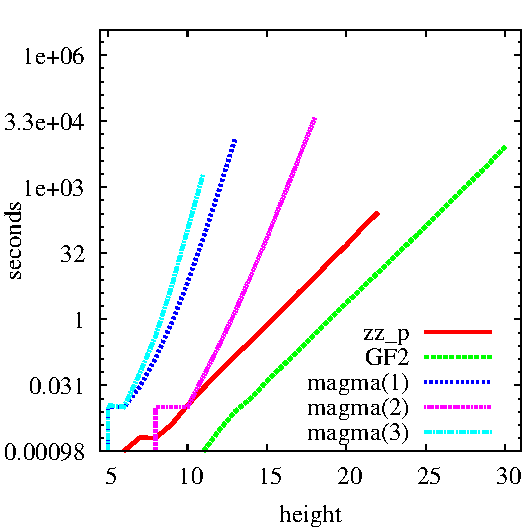
\includegraphics[height=0.5\textwidth]{artin/build1}
  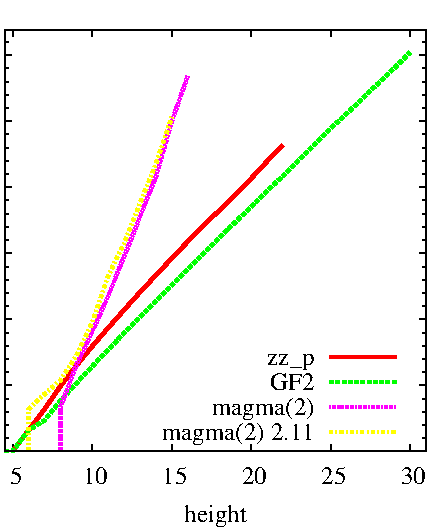
\includegraphics[height=0.5\textwidth]{artin/iso1}
  
  \caption{Build time (left) and isomorphism time (right) with respect to tower height. Plot is in logarithmic scale.}
  \label{fig:height}
\end{figure}

\begin{figure}
  \centering
  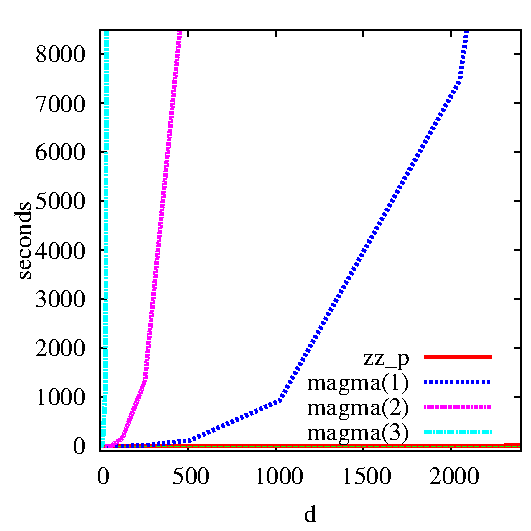
\includegraphics[height=0.5\textwidth]{artin/build-d}
  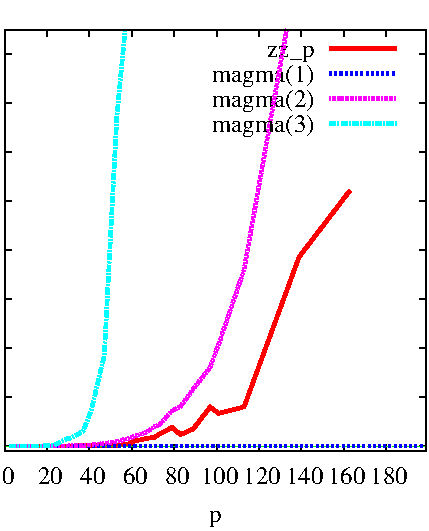
\includegraphics[height=0.5\textwidth]{artin/build-p}
  
  \caption{Build times with respect to $d$ (left) and $p$ (right).}
  \label{fig:p-d}
\end{figure}

\pdfmcthree{A little comment on magma(2) for p increasing.}
The timings of our code are significantly better for increasing height
or increasing $d$. Not surprisingly, for increasing $p$, the magma(1)
approach performs better than any other: the \texttt{quo} operation
simply creates a residue class ring, regardless of the
(ir)reducibility of the modulus, so the timing for building two levels
barely depend on $p$. The most adapted approach for this situation
presumably is magma(2); yet we notice that \texttt{FAAST} has
reasonable performances for characteristics up to about $p=50$.

In Tables~\ref{tab:arith-gf2} and~\ref{tab:arith-zzp} we provide some
comparative timings for the different arithmetic operations provided
by \texttt{FAAST}. The column ``Primitive'' gives the time taken to
build one level of the primitive tower (this includes the
precomputation of the data as described in
Subsection~\ref{sec:level-embedding:lift-up}); the other entries are
self-explanatory. Product and inversion are just wrappers around
\texttt{NTL} routines: in these operations we did not observe any
overhead compared to the native \texttt{NTL} code. All the operations
stay within a factor of $30$ of the cost of multiplication, which is
satisfactory.

\begin{table}
  \centering
  \begin{tabular}{l r r r r r r r}
    \hline
    \small level & \small Primitive & \small Push-d. & \small Lift-up & \small Product & \small Reciprocal & \small apply $\sigma^{-1}$ & \small apply $\sigma$ \\
    \hline
    19 &  1.143 & 0.304 &  1.265 & 0.039 &  0.649 &  0.652 &  1.290\\
    20 &  2.566 & 0.609 &  2.796 & 0.081 &  1.544 &  1.314 &  2.602\\
    21 &  5.686 & 1.225 &  6.147 & 0.187 &  3.598 &  2.409 &  2.668\\
    22 & 12.660 & 2.515 & 13.746 & 0.463 &  8.355 &  5.565 & 11.179\\
    23 & 28.511 & 5.295 & 31.200 & 1.046 & 19.522 & 12.323 & 24.740
  \end{tabular}
  \caption{Some timings in seconds for arithmetics in a generic tower built over $\F_2$ using \texttt{GF2}.}
  \label{tab:arith-gf2}
\end{table}

\begin{table}
  \centering
  \begin{tabular}{l r r r r r r r}
    \hline
    \small level & \small Primitive & \small Push-d. & \small Lift-up & \small Product & \small Reciprocal & \small $\sigma^{-1}$ & \small  $\sigma$ \\
    \hline
    18 &  13.618 &  0.884 &  13.712 & 0.476 &  10.753 &  1.337 &  3.578\\
    19 &  30.288 &  1.814 &  30.432 & 1.001 &  23.046 &  2.850 &  7.798\\
    20 &  65.632 &  3.953 &  66.889 & 2.106 &  51.544 &  6.564 & 18.141\\
    21 & 128.190 &  8.347 & 131.271 & 4.791 & 121.349 & 14.396 & 39.296\\
    22 & 296.671 & 11.396 & 298.541 & 6.413 & 249.520 & 28.851 & 86.628
  \end{tabular}
  \caption{Some timings in seconds for arithmetics in a generic tower built over $\F_2$ using \texttt{zz\_p}.}
  \label{tab:arith-zzp}
\end{table}


Finally, we mention the cost of precomputation. The precomputation of
the images of $\sigma$ as explained in
Section~\ref{sec:couveignes-algorithm} is quite expensive; most of it
is spent computing pseudotraces. Indeed it took one week to precompute
the data in Figure~\ref{fig:height} (right), while all the other data
can be computed in a few hours. There is still space for some minor
improvement in \texttt{FAAST}, mainly tweaking recursion thresholds
and implementing better algorithms for small and moderate input
sizes. Yet we think that only a major algorithmic improvement could
consistently speed up this phase.



% Local Variables: 
% mode:flyspell
% ispell-local-dictionary:"american"
% TeX-master: "../these"
% mode: TeX-PDF
% mode: reftex
% End: 
%
% LocalWords:  univariate isogeny Couveignes isogenies Artin Schreier



% Local Variables:
% mode:flyspell
% ispell-local-dictionary:"american"
% mode:TeX-PDF
% mode:reftex
% TeX-master: "../these"
% End:

\part{Applications to isogeny computation and cryptology}
\label{part:appl-isog-comp}
\chapter{Elliptic curves and isogenies}
Elliptic curves and bla and bla and bla. See
\cite{silverman:elliptic,silverman:advanced,blake+seroussi+smart,milne1996elliptic,connell:elliptic}.

\section{Definitions}
\label{sec:definitions}

We let $\K$ be a field and $\clot{\K}$ be its algebraic
closure. \index{elliptic~curve}Elliptic curves are genus $1$ curves
over $\clot{\K}$ with a distinguished point.

\subsection{Weierstrass equations}
\label{sec:weierstr-equat}

\begin{definition}[Weierstrass equation]
  \index{Weierstrass~equation} Any elliptic curve $E$ can be viewed as
  the projective variety associated to the equation
  \begin{equation}
    \label{eq:107}
    E\;:\; Y^2Z + a_1XYZ + a_3YZ^2 = X^3 + a_2X^2Z + a_4XZ^2 + a_6Z^3
    \text{,}
  \end{equation}
  with $a_1,\ldots,a_6\in\clot{\K}$.  The distinguished point is
  $[0:1:0]$, called the \index{point~at~infinity}\emph{point at
    infinity} and denoted by $\0$\nomenclature[O]{$\0$}{Point at
    infinity of an elliptic curve}.  When $a_1,\ldots,a_6\in\K$, the
  curve is said to be \emph{defined over $\K$}.
\end{definition}

Eq.~\eqref{eq:107} is called the \emph{homogeneous Weierstrass
  form}\index{Weierstrass~form!homogeneous} of the curve $E$.  After
the change of variables $x=\frac{X}{Z},y=\frac{Y}{Z}$,
Eq.~\eqref{eq:107} can be rewritten as
\begin{equation}
  \label{eq:112}
  E\;:\;y^2 + a_1xy + a_3y = x^3 + a_2x^2 + a_4x + a_6
  \text{,}
\end{equation}
called the \emph{affine Weierstrass
  form}\index{Weierstrass~form!affine}. Then the curve $E$ is the
locus of zeros of Eq.~\eqref{eq:112} in $\clot{\K}^2$ (or, more
exactly, in the affine plane $\mathbb{A}^2$), plus the extra point at
infinity $\0$.

\begin{definition}[Function field]
  If $E$ is an elliptic curve defined by an affine Weierstrass
  equation $f(x,y)=0$ with coefficients in $\K$, we denote by $\K(E)$%
  \nomenclature[KE]{$\K(E)$}{Function field of an elliptic curve} the
  field of fractions of
  \begin{equation}
    \label{eq:125}
    K[E]=K[x,y]/(f(x,y))
    \text{,}
  \end{equation}
  and call it the \index{function~field}\emph{function field} of $E$
  over $\K$.
\end{definition}

The \index{discriminant~of~an~elliptic~curve}discriminant of
Eq.~\eqref{eq:112} is
\begin{equation}
  \label{eq:118}
  \Delta_E = -b_2^2b_8-8b_4^3-27b_6^2+9b_2b_4b_6
  \text{,}
\end{equation}
where
\begin{equation}
  \label{eq:117}
  \begin{aligned}
    b_2 &= a_1^2 + 4a_2\text{,}\\
    b_4 &= 2a_4 + a_1a_3\text{,}\\
    b_6 &= a_3^2 + 4a_6\text{,}\\
    b_8 &= a_1^2a_6+4a_2a_6-a_1a_3a_4+a_2a_3^2-a_4^2\text{.}
  \end{aligned}
\end{equation}

\begin{remark}
  The curve defined by~\eqref{eq:112} has an unique singular point if
  and only if $\Delta_E=0$.  Figure~\ref{fig:singular} shows the two
  possible shapes of a singular curve over the reals. Then, every line
  passing through the singular point meets the curve in another unique
  point. This parameterization makes $E$ birationally equivalent to
  $\Proj^1$, thus $E$ has genus $0$. The converse is also true, thus
  Eq.~\eqref{eq:112} defines an elliptic curve if and only if
  $\Delta_E\ne0$.
\end{remark}


\begin{figure}[ht]
  \centering
  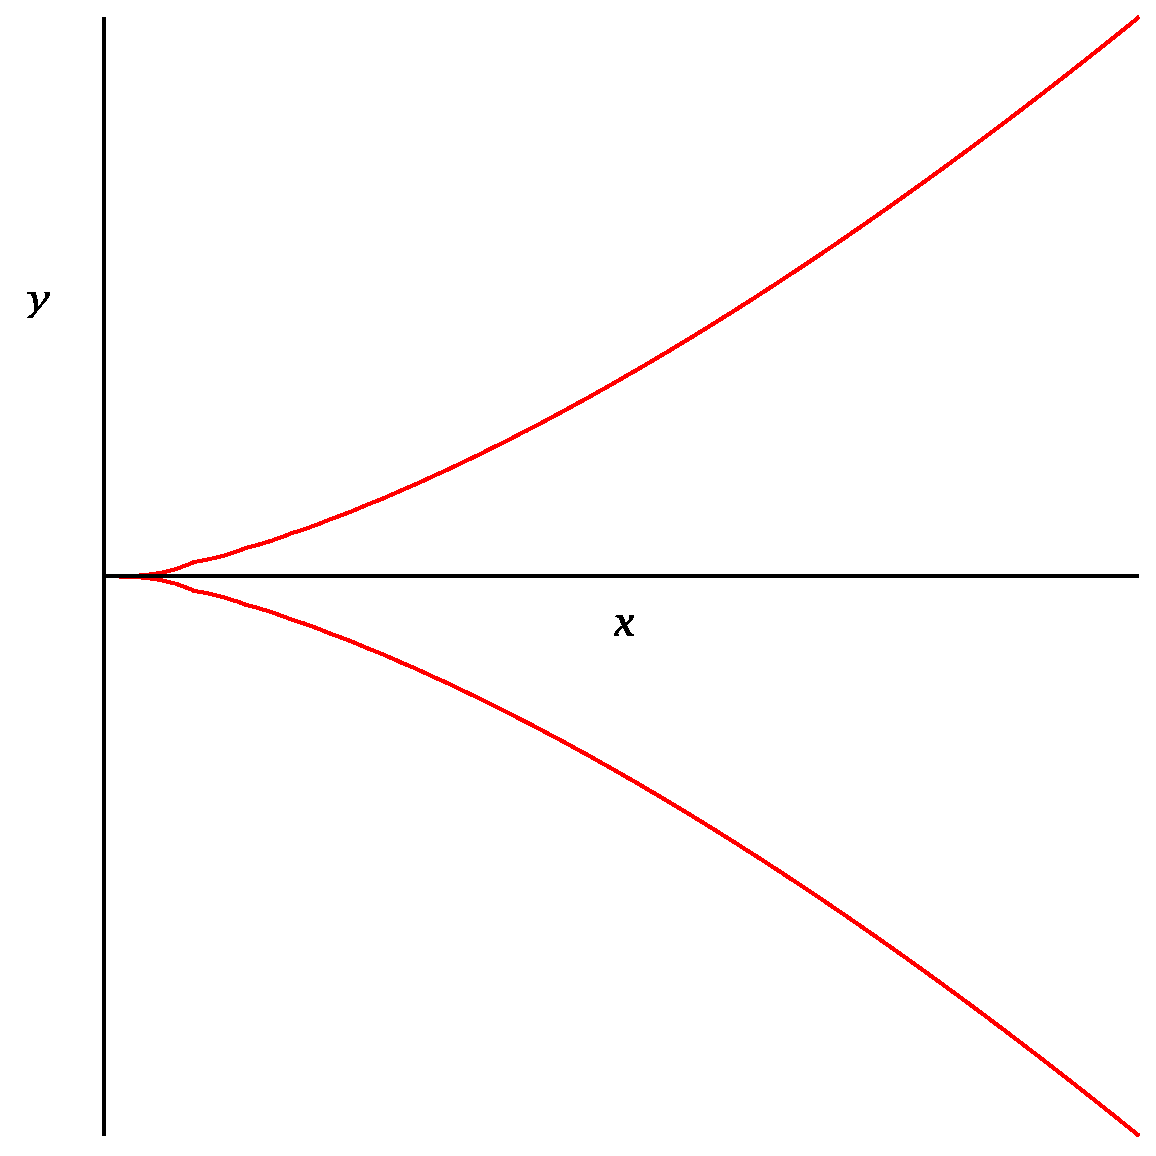
\includegraphics[width=0.45\textwidth]{isogeny/cusp}
  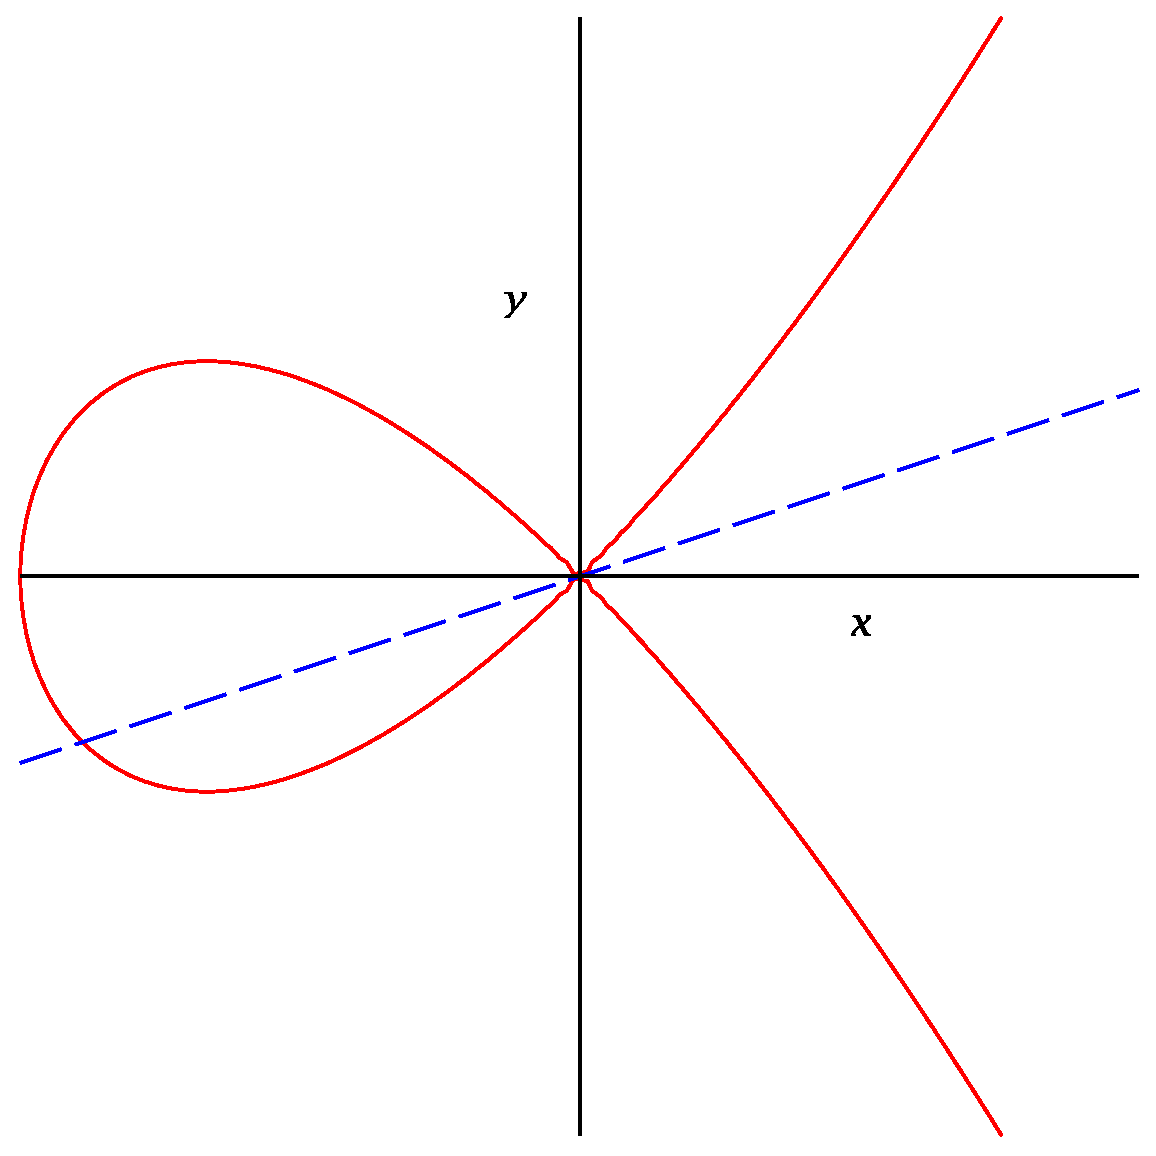
\includegraphics[width=0.45\textwidth]{isogeny/node}
  \caption{Two singular Weierstrass curves. On the left $y^2=x^3$, on
    the right $y^2=x^3+x^2$. On the right we have shown the
    parameterization by the line passing through the origin.}
  \label{fig:singular}
\end{figure}

\begin{definition}[$j$-invariant]
  \index{j-invariant@$j$-invariant}%
  \nomenclature[j]{$j_E$}{$j$-invariant of an elliptic curve $E$}
  We associate to the curve $E$ defined by Eq.~\eqref{eq:112}, the
  $j$-invariant
 \[j_E = \frac{(b_2^2-24b_4)^3}{\Delta_E}\text{.}\]
\end{definition}


\subsection{Group law}
\label{sec:group-law}
Elliptic curves are endowed with a group structure via the
\index{elliptic~curve!group~law}
\index{chord-tangent~law}\emph{chord-tangent law}.

\begin{definition}
  Let $E$ be an elliptic curve and let $P,Q\in\Proj^2$ be two points
  on the curve. Let $L$ be the line passing through $P$ and $Q$, with
  multiplicity two if $P=Q$, and let $R$ be the third intersection
  point with $E$.  Let $L'$ be the line passing through $R$ and
  $\0$. Then the point $P+Q$ is defined as the third point of
  intersection of $L'$ and $E$.
\end{definition}

\begin{figure}[ht]
  \centering
  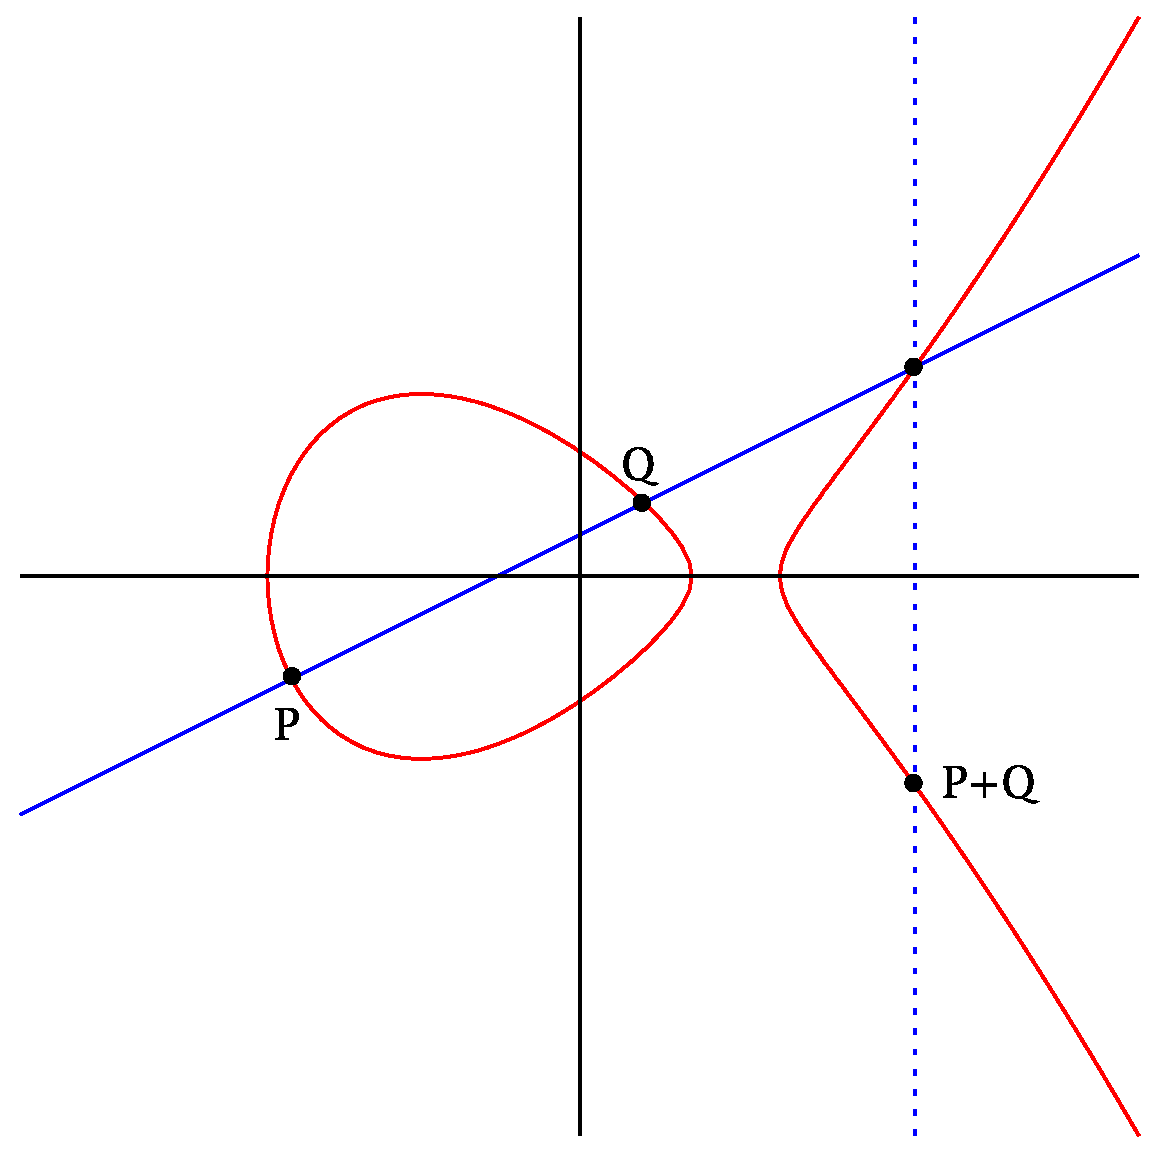
\includegraphics[width=0.5\textwidth]{isogeny/ec-add}
  \caption{Chord-tangent law on an elliptic curve defined over the reals.}
  \label{fig:chord-tangent}
\end{figure}

The definition is pictured in Figure~\ref{fig:chord-tangent}. For a
proof that this defines indeed a group law on the points of $E$, with
$\0$ being the identity element, see \cite[II, $\S2$]{silverman:elliptic}.

\begin{definition}[Rational points]%
  \nomenclature[E]{$E(\K)$}{Set of $\K$-rational points of an elliptic curve $E$}
  Let $E$ be an elliptic curve defined over $\K$, the set of
  \emph{$\K$-rational points}\index{rational~point} $E(\K)$ is 
  \begin{equation}
    \label{eq:119}
    E(\K) = E \cap \Proj^2(\K)
    \text{.}
  \end{equation}
\end{definition}

If $P$ and $Q$ are rational points, the lines $L$ and $L'$ are defined
by equations over $\K$, thus $E(\K)$ forms a subgroup of $E$. To allow
calculations in $E(\K)$ without having to lift the coefficients in an
algebraic closure, it is convenient to give explicit formulas for the
chord-tangent law. 

We shall give the formulas for affine coordinates. From now on, if $P$
is an affine point of $E$, we denote by $x(P)$ its abscissa and by
$y(P)$ its ordinate.

\begin{proposition}
  Let $E$ be the elliptic curve defined by Eq.~\eqref{eq:112}. Let
  $P$, be a point of $E$ different from $\0$, the coordinates of $-P$
  are given by
  \begin{equation}
    \label{eq:120}
    x(-P) = x(P)\text{,}\qquad y(-P)=-y(P) -a_1x(P) - a_3
    \text{.}
  \end{equation}
  Let $P,Q$ be points of $E$ different from $\0$ and let $Q\ne-P$, the
  coordinates of $P+Q$ are given by
  \begin{equation}
    \label{eq:121}
    \begin{aligned}
      \lambda &= \begin{cases}
        \frac{y(Q) - y(P)}{x(Q) -x(P)} &\text{if $P\ne Q$,}\\
        \frac{3x(P)^2+2a_2x(P)+a_4-a_1y(P)}{2y(P)+a_1x(P)+a_3} &\text{if $P=Q$,}
      \end{cases}\\
      x(P+Q) &= \lambda^2+a_1\lambda-a_2-x(P)-x(Q)\text{,}\\
      y(P+Q) &= -(\lambda+a_1)x(P+Q) - y(P) + \lambda x(P)-a_3\text{.}
    \end{aligned}
  \end{equation}
\end{proposition}

\begin{definition}[Kummer surface]
  The \index{Kummer~surface}\emph{Kummer surface} of an elliptic curve
  $E$, denoted by $K_E$\nomenclature[KE]{$K_E$}{Kummer surface of an
    elliptic curve}, is the quotient of $E$ by the equivalence
  relation $P\simeq-P$.
\end{definition}

For $m\in\Z$, we denote by $[m]P$ the point%
\nomenclature[mP]{$[m]P$}{Scalar multiple of a point of an elliptic
  curve} $\overbrace{P+P+\cdots+P}^{m\text{ times}}$ if $m>0$, or the
point $[-m](-P)$ if $m<0$, or $\0$ if $m=0$. 

\begin{remark}
  The Kummer surface can be represented by taking the abscissas of the
  points of $E$. It is not anymore a group, but we can still compute
  scalar multiples of its points. In fact, from the addition formulas
  we deduce for $P\ne-P$
  \begin{equation}
    \label{eq:128}
    x([2]P) = \frac{x^4-b_4x^2-2b_6x-b_8}{4x^3+b_2x^2+2b_4x+b_6}
    \text{,}
  \end{equation}
  where $x=x(P)$; and for $P\ne Q$
  \begin{equation}
    \label{eq:129}
    x(P+Q) + x(P-Q) =
    \frac{2\pi\sigma + b_2\pi + b_4\sigma + b_6}{(x(P)-x(Q))^2}
    \text{,}
  \end{equation}
  where $\pi=x(P)x(Q)$ and $\sigma=x(P)+x(Q)$. 

  Then, to compute $x([n]P)$, we start from $x(P)$ and $x([2]P)$, and
  we iteratively apply
  \begin{equation}
    \label{eq:130}
    \begin{aligned}[]
      [2i]P   &= [2][i]P\text{,}\\
      [2i+1]P &= [i+1]P + [i]P\text{,}
    \end{aligned}
  \end{equation}  
  or
  \begin{equation}
    \label{eq:131}
    \begin{aligned}[]
      [2i+1]P &= [i+1]P + [i]P\text{,}\\
      [2i+2]P &= [2][i+1]P\text{,}
    \end{aligned}
  \end{equation}
  until we reach $[n]P$. This algorithm appeared
  in~\cite{montgomery87} and is sometimes referred to as
  \index{Montgomery's formulas}\emph{Montgomery's formulas}.
\end{remark}

The map
\begin{equation}
  \label{eq:122}
  \begin{aligned}[]
    [m]_E : E(\K) &\ra E(\K)\text{,}\\
    P &\mapsto [m]P
  \end{aligned}
\end{equation}
is a group endomorphisms of $E(\K)$. 

\begin{definition}
  The $m$-th \emph{torsion subgroup} of $E$ is
  \begin{equation}
    \label{eq:123}
    E[m] = \{P\in E(\K) \,|\, [n]P=\0\}
    \text{,}
  \end{equation}
  its points are called%
  \nomenclature[E]{$E[m]$}{$m$-torsion subgroup of an elliptic curve
    $E$}
  \index{elliptic~curve!torsion~subgroup}\index{torsion~point}\emph{$m$-torsion
    points}.
\end{definition}

Since addition is an algebraic map, multiplication by $n$ is algebraic
too. It can be shown that there exist polynomials
$\psi_m,\theta_m,\omega_m\in\K(E)$ such that
\begin{equation}
  \label{eq:124}
  [m](x,y) = \left(\frac{\theta_m(x,y)}{\psi_m(x,y)^2},
    \frac{\omega_m(x,y)}{\psi_m(x,y)^3}\right)
  \text{.}
\end{equation}

\begin{definition}[Division polynomials]
  The polynomial $\psi_m$ is called the
  \index{division~polynomial}\emph{$m$-th division polynomial}.
\end{definition}

\begin{remark}
  The division polynomials can be computed from the addition formulas
  via a double-and-add approach. Their importance comes from the fact
  that $\psi_m$ vanishes on $E[m]$.
\end{remark}

From the formulas for the division polynomials one can deduce the
structure of the $m$-torsion.

\begin{theorem}
  Let $p$ be the characteristic of $\K$. If $p$ does not divide $m$
  \begin{equation}
    \label{eq:126}
    E[m] \isom \Z/m\Z\times\Z/m\Z
    \text{;}
  \end{equation}
  if $p\ne0$, then for every $i>0$ either
  \begin{equation}
    \label{eq:127}
    E[p^i] = \{\0\}\text{,} 
    \qquad\text{or}\qquad E[p^i] \isom \Z/p^i\Z
    \text{.}
  \end{equation}
\end{theorem}

\begin{definition}[Supersingular, ordinary]
  An elliptic curve $E$ is said to be
  \index{elliptic~curve!supersingular}\index{supersingular}\emph{supersingular}
  if $E[p^i]=\{\0\}$ for any $i$; it is said to be
  \index{elliptic~curve!ordinary}\emph{ordinary} otherwise.
\end{definition}

\begin{definition}[Tate module]
  Let $\ell$ be a prime, the \index{Tate~module}\emph{$\ell$-adic Tate
    module}
  $\mathcal{T}_\ell(E)$\nomenclature[Tl]{$\mathcal{T}_\ell(E)$}{$\ell$-adic
    Tate module} is the group
  \begin{equation}
    \label{eq:132}
    \mathcal{T}_\ell(E) = \varprojlim_n E[\ell^n]
  \end{equation}
  with respect to the projections
  \begin{equation}
    \label{eq:133}
    [\ell]_E : E[\ell^{n+1}] \ra E[\ell^{n}]
    \text{.}
  \end{equation}
\end{definition}

\begin{proposition}
  The Tate module has a natural structure of
  $\Z_\ell$-module\nomenclature[Zp]{$\Z_p$}{$p$-adic
    integers\nomnorefpage}. As such
  \begin{equation}
    \label{eq:134}
    \mathcal{T}_\ell(E) \isom
    \begin{cases}
      \Z_\ell\times\Z_\ell &\text{if $\ell\ne p$,}\\
      \Z_p &\text{if $\ell=\car(\K)$ and $E$ is ordinary,}\\
      \{\0\} &\text{if $E$ is supersingular.}
    \end{cases}
  \end{equation}
\end{proposition}


\subsection{Isomorphisms}
\label{sec:isomorphisms}

Let $E$ and $E'$ be two elliptic curves in Weierstrass form over a
field $\K$, they are said to be isomorphic if there is a linear change
of variables that transforms one equation in the other and preserves
the point at infinity.  Then, clearly $E(\clot{\K})$ and
$E'(\clot{\K})$ are isomorphic as groups. If the change of variables
has coefficients in $\K$, the curves are said to be
\index{isomorphism!of~elliptic~curves}\index{elliptic~curve!isomorphic}isomorphic
over $\K$, then $E(\K)$ and $E(\K)$ are isomorphic as groups.

It can be shown that the only such changes of variables are
\begin{equation}
  \label{eq:116}
  \begin{aligned}
    x &= u^2x' + r\text{,}\\
    y &= u^3y' + u^2sx' + t\text{,}
  \end{aligned}
\end{equation}
with $r,s,t,u\in\clot{\K}$.

\begin{proposition}
  Two elliptic curves $E$ and $E'$ in Weierstrass form are isomorphic
  over $\clot{\K}$ if and only if $j_E=j_{E'}$.
\end{proposition}

\index{Weierstrass~form!simplified~form}Weierstrass equations can be
brought via isomorphism to a form that is easier to handle, called
\emph{simplified Weierstrass form}. The following classification is
from~\cite{connell:elliptic}.

\begin{proposition}[Simplified Weierstrass form]
  Any elliptic curve is isomorphic to one of the following Weierstrass
  forms:
  \begin{itemize}
  \item If $\car(\K)=0$ or $\car(\K)>3$
    \begin{equation}
      \label{eq:weierstrass>3}
      E\;:\;y^2 = x^3 + ax + b 
      \qquad\text{and}\qquad
      j_E = \frac{1728(4a)^3}{16(4a^3 + 27b^2)}
      \text{;}
    \end{equation}
  \item if $\car(\K)=3$ and $E$ is ordinary
    \begin{equation}
      \label{eq:weierstrass=3}
      E\;:\;y^2 = x^3 + ax^2 + b
      \qquad\text{and}\qquad
      j_E = -\frac{a^3}{b}
      \text{;}
    \end{equation}
  \item if $\car(\K)=3$ and $E$ is supersingular
    \begin{equation}
      \label{eq:136}
      E\;:\;y^2=x^3 + ax+b
      \qquad\text{and}\qquad
      j_E=0
      \text{;}
    \end{equation}
  \item if $\car(\K)=2$ and $E$ is ordinary
    \begin{equation}
      \label{eq:weierstrass=2}
      y^2 + xy = x^3 + ax^2 + b
      \qquad\text{and}\qquad
      j_E = \frac{1}{b}
      \text{;}
    \end{equation}
  \item if $\car(\K)=2$ and $E$ is supersingular
    \begin{equation}
      \label{eq:137}
      E\;:\; y^2 + a_3y = x^3 + a_4x + a_6
      \qquad\text{and}\qquad
      j_E = 0
      \text{.}
    \end{equation}
  \end{itemize}
\end{proposition}

\begin{definition}[Twist]
  Two non-isomorphic elliptic curves $E$ and $E'$ over $\K$ such that
  $j_E=j_{E'}$ are called \index{twist}\emph{twists}.
\end{definition}

A twist is isomorphic over the algebraic closure $\clot{\K}$. The
\index{twist!degree~of~a}degree of the twist is the degree of the
smallest extension $\K'/\K$ such that the twist is isomorphic over
$\K$.

\begin{proposition}
  Any curve has a quadratic twist. Any twist of ordinary elliptic
  curves is quadratic.
\end{proposition}


\subsection{Isogenies}
\label{sec:isogenies}

\begin{definition}[Isogeny]
  Let $E$ and $E'$ be elliptic curves, an
  \index{isogeny}\emph{isogeny} $E\ra E$ is a morphism of varieties
  that preserves the point at infinity.
\end{definition}

It turns out that isogenies preserve the group structure.

\begin{theorem}
  Let $\I:E\ra E'$ be an isogeny, then it is a group morphism
  $E(\clot{\K})\ra E'(\clot{\K})$. It is surjective and its kernel is
  finite. Furthermore, if $\I$ is defined over $\K$, then its
  restriction to $E(\K)$ is a group morphism $E(\K)\ra E'(\K)$.
\end{theorem}

\begin{definition}[Degree]
  Let $\I$ be an isogeny and
  \index{degree!of~an~isogeny}\index{isogeny!degree}define
  \begin{equation}
    \label{eq:138}
    \begin{aligned}
      \dual{\I}:\clot{K}(E')&\ra\clot{K}(E)\\
      f &\ra f\circ\I
      \text{.}
    \end{aligned}
  \end{equation}
  The \emph{separable (resp. inseparable) degree} of $\I$, denoted by
  $\deg_s\I$ (resp. $\deg_i\I$), is the separable (resp. inseparable)
  degree of the field extension $\clot{\K}(E)/\I(\clot{\K}(E'))$. The
  \emph{degree} of $\I$ is $\deg\I=\deg_s\I\deg_i\I$.

  An isogeny is called \index{isogeny!separable}\emph{separable} if
  $\deg_i\I=1$, \index{isogeny!inseparable}\emph{inseparable}
  otherwise. It is called
  \index{isogeny!purely~inseparable}\emph{purely inseparable} if
  $\deg_s=1$.
\end{definition}

\begin{theorem}
  Let $\I$ be an isogeny, its kernel contains $\deg_s\I$ elements.
\end{theorem}

One example of isogeny is the map $[m]$, it is a separable isogeny of
degree $m^2$. If $\K$ has characteristic $p$, then the map
\begin{equation}
  \label{eq:139}
  \frobisog : (x,y) \mapsto (x^p,y^p)
\end{equation}
is a purely inseparable isogeny of degree $p$, called the
\index{Frobenius~isogeny}\emph{Frobenius
  isogeny}\nomenclature[f]{$\frobisog$}{Frobenius isogeny:
  $(x,y)\mapsto(x^p,y^p)$}. If $\K$ is a perfect field, any purely
inseparable isogeny is a power of $\frobisog$.

\begin{theorem}
  Any isogeny can be factored in a product of a separable and a purely
  inseparable isogeny.
\end{theorem}

One important property about isogenies is that they factor the
multiplication by $m$ map.

\begin{definition}[Dual isogeny]
  Let $\I : E \rightarrow E'$ be a degree $m$ isogeny. There exists an
  unique isogeny $\hat{\I} : E' \rightarrow E$, called the
  \index{dual~isogeny}\index{isogeny!dual}\emph{dual isogeny} such
  that
  \[\I\circ\hat{\I} = [m]_E \qquad\text{and}\qquad \hat{\I}\circ\I =
  [m]_{E'}\]
\end{definition}

By endomorphism we mean an isogeny $E\ra E$. The multiplication maps
are endomorphisms, thus $\End(E)$ contains a copy of $\Z$.  The main
theorem about the endomorphism ring $\End(E)$ is the following.

\begin{theorem}
  The endomorphism ring is either isomorphic to $\Z$, or to an order
  in a quadratic imaginary field, or to an order in a quaternion
  algebra.
\end{theorem}

If $\car(\K)\ne0$, we can exclude the case $\Z$, because $\End(E)$
contains the Frobenius isogeny. Furthermore, in the two cases
\begin{itemize}
\item $\car(\K)=0$,
\item $\K$ perfect and $E$ ordinary
\end{itemize}
$\End(E)$ cannot be an order in a quaternion algebra, thus it is
commutative.


\section{Curves over $\C$}
\label{sec:curves-over-c}
Elliptic curves defined over $\C$ have a very simple structure.

\begin{definition}[Lattice]
  A \index{lattice}\emph{lattice} $\Lambda\subset\C$ is a discrete
  additive subgroup of $\C$ that contains a basis of the $\R$-vector
  space $\C$. Two lattices $\Lambda_1,\Lambda_2$ are said to be
  \emph{homothetic} if $\Lambda_1=\alpha\Lambda_2$ for some
  $\alpha\in\C^{\ast}$.
\end{definition}

\begin{definition}[Elliptic function]
  Let $\Lambda$ be a lattice. An
  \index{elliptic~function}\emph{elliptic function} on $\Lambda$ is a
  meromorphic function $f$ on $\C$ such that
  \begin{equation}
    \label{eq:141}
    f(z+\omega) = f(z)
  \end{equation}
  for any $\omega\in\Lambda$.  The set of elliptic functions on
  $\Lambda$ is denoted by $\C(\Lambda)$.
\end{definition}

An example of elliptic function is the
\index{Weierstrass~function@Weierstrass~$\wp$-function}\emph{Weierstrass
  $\wp$-function}\nomenclature[p]{$\wp$}{Weierstrass $\wp$-function}
\begin{equation}
  \label{eq:142}
  \wp(z;\Lambda) = \frac{1}{z^2} + \sum_{\omega\in\Lambda\backslash\{0\}}\frac{1}{(z-\omega)^2}-\frac{1}{\omega^2}
  \text{,}
\end{equation}
\begin{theorem}
  Let $\Lambda$ be a lattice, then $\C(\Lambda) = \C(\wp(z),\wp'(z))$.
\end{theorem}

For $k>1$, we define the \index{Eisenstein~series}\emph{Eisenstein
  series} $G_{2k}$\nomenclature[G2k]{$G_{2k}$}{Eisenstein series} as
\begin{equation}
  \label{eq:143}
  G_{2k}(\Lambda) = \sum_{\omega\in\Lambda\backslash\{0\}}\frac{1}{\omega^2}
  \text{.}
\end{equation}

\begin{theorem}
  The Laurent series expansion of $\wp(z)$ at $0$ is
  \begin{equation}
    \label{eq:144}
    \wp(z) = \frac{1}{z^2} + \sum_{k=1}^\infty (2k+1)G_{2k+2}z^{2k}
    \text{.}
  \end{equation}
  At any $z\not\in\Lambda$, the function $\wp(z)$ satisfies the
  differential equation
  \begin{equation}
    \label{eq:145}
    {\wp'}^2 = 4\wp - 60G_4\wp - 140G_6
    \text{.}
  \end{equation}
\end{theorem}

We set $g_2(\Lambda)=60G_4(\Lambda)$ and $g_3(\Lambda)=140G_6(\Lambda)$.

\begin{theorem}
  Let $E$ be the curve 
  \begin{equation}
    \label{eq:146}
    E\;:\: y^2=4x^3-g_2(\Lambda)x-g_3(\Lambda)
    \text{.}
  \end{equation}
  The map
  \begin{equation}
    \label{eq:147}
    \begin{aligned}
      \phi: \C/\Lambda &\ra E(\C)\\
      z &\mapsto
      \begin{cases}
        \0 &\text{if $z=0$,}\\
        (\wp(z), \wp'(z)) &\text{otherwise,}
      \end{cases}
    \end{aligned}
  \end{equation}
  is an isomorphism of Riemann surfaces and a group homomorphism. 
\end{theorem}

If $\Lambda$ is a lattice, we denote by $E_\Lambda$ the elliptic curve
corresponding to it as in Eq.~\eqref{eq:146}.

\begin{theorem}
  Let $\Lambda_1,\Lambda_2$ be lattices and let $a\in\C^\ast$ such that
  $a\Lambda_1\subset\Lambda_2$. The map
  \begin{equation}
    \label{eq:148}
    \begin{aligned}
      \phi_a:\C/\Lambda_1&\ra\C/\Lambda_2\\
      z&\mapsto az
    \end{aligned}
  \end{equation}
  is holomorphic. The map $E_{\Lambda_1}\ra E_{\Lambda_2}$ induced by
  $\phi_a$ is an isogeny.
\end{theorem}

The correspondences we just defined are actually equivalences.

\begin{theorem}
  The category of elliptic curves with isogenies as maps is equivalent
  to the category of lattices up to homothety with maps $z\mapsto az$
  such that $a\Lambda_1\subset\Lambda_2$.
\end{theorem}

Thus to any elliptic curve there is an unique lattice $\Lambda$
associated up to homothety; the addition law on $\C/\Lambda$ is just
addition in $\C$, and an isogeny can be obtained by an $a\in\C$ such
that $a\Lambda_1\subset\Lambda_2$.



\section{Curves over finite fields}
\label{sec:curves-over-finite}
We saw previously that an elliptic curve defined over a field of
characteristic $p\ne0$ has an isogeny
\begin{equation}
  \label{eq:150}
  \frobisog:(x,y)\mapsto(x^p,y^p)
\end{equation}
called Frobenius isogeny. If the curve $E$ is defined over the field
$\F_q$ with $q=p^d$, then $d$ iterations of the Frobenius map give the
isogeny
\begin{equation}
  \label{eq:151}
  \frobisog_q\eqdef\frobisog^d:(x,y)\mapsto(x^q,y^q)
  \text{.}
\end{equation}

The map $\frobisog_q$ is an endomorphism of $E$ and fixes the points
of $E(\F_q)$; it is called the \index{Frobenius
  endomorphism}\emph{Frobenius endomorphism} of $E$. It plays an
important role in determining the cardinality of $E(\F_q)$.

\begin{theorem}[Hasse]
  \index{Hasse~bound}
  The minimal polynomial of $\frobisog_q$ in $\End(E)$ is of the form
  \begin{equation}
    \label{eq:152}
    \frobisog_q^2 - c\frobisog_q + q = 0
  \end{equation}
  with $\lvert c\rvert\le2\sqrt{q}$.
\end{theorem}

Since $\frob_q$ acts as the identity on $E(\F_q)$, this implies
\begin{equation}
  \label{eq:153}
  \card{E(\F_q)} = q+1-c
  \qquad\text{with } \lvert c\rvert\le2\sqrt{q}
  \text{.}
\end{equation}

\begin{theorem}
  Two elliptic curves $E,E'$ defined over $\F_q$ are isogenous if and
  only if $\card{E(\F_q)}=\card{E(\F_q)}$.
\end{theorem}


\section{Vélu formulas}
\label{sec:velu-formulas}
For any finite subgroup $G \subset E(\clot{\K})$, Vélu formulas
\cite{Vel71} give in a canonical way an elliptic curve $\bar{E}$ and
an explicit isogeny $\I:E\rightarrow \bar{E}$ such that
$\ker\I=G$. The isogeny is $\K$-rational if and only if the polynomial
vanishing on the abscissae of $G$ belongs to $\K[X]$.

In practice, if $E$ is defined over $\F_q$ and if
\[h(X) = \prod_{\substack{P\in G\\P\ne\0}}(X - x(P)) \in \F_q[X]\]
is known, Vélu formulas compute a rational function
\begin{equation}
  \label{eq:isog}
  \bar{\I}(x,y) = \left(\frac{g(x)}{h(x)}, \frac{k(x,y)}{l(x)}\right)  
\end{equation}
and a curve $\bar{E}$ such that $\bar{\I} : E\rightarrow\bar{E}$ is an
$\F_q$-rational isogeny of kernel $G$. A consequence of Vélu formulas
is
\begin{equation}
  \label{eq:velu-deg}
  \deg g = \deg h + 1 = \card{G}
  \text{.}
\end{equation}

Given two curves $E$ and $E'$, Vélu formulas reduce the problem of
finding an explicit isogeny between $E$ and $E'$ to that of finding
the kernel of an isogeny between them. Once the polynomial $h(X)$
vanishing on $\ker\I$ is found, the explicit isogeny is computed
composing Vélu formulas with the isomorphism between $\bar{E}$ and
$E'$ as in figure \ref{fig:velu}.

\begin{figure}
  \centering
  \[\xymatrix{
    E \ar[r]^{\bar{\I}} \ar[rd]^\I & \bar{E} \ar[d]^{\simeq}\\
    & E'
  }\]
  \caption{Using Vélu formulas to compute an explicit isogeny.}
  \label{fig:velu}
\end{figure}





% Local Variables:
% mode:flyspell
% ispell-local-dictionary:"american"
% mode:TeX-PDF
% mode:reftex
% TeX-master: "../these"
% End:
%
% LocalWords:  Schreier Artin pseudotrace frobenius bivariate Joux Sirvent FFT
% LocalWords:  Couveignes isogenies Schoof isogeny cryptosystems Lercier
% LocalWords:  precomputation arithmetics polylogarithmic Karatsuba
% LocalWords:  endomorphisms


\chapter{Computing isogenies over finite fields}
\label{cha:algor-small-char}
%\section{Couveignes first algorithm}
%\section{Lercier}
%% these.tex
%% Copyright 2010 Luca De Feo
%% All rights reserved


Let $E$ and $E'$ be two elliptic curves defined over $\K$, by finding
an \emph{explicit isogeny} we mean to find an ($\F_q$-rational)
rational function from $E(\clot{\K})$ to $E'(\clot{\K})$ such that the
map it defines is an isogeny. 

In this chapter we are interested in finding explicit isogenies of
ordinary elliptic curves over finite fields. In what follows $\F_q$
will be a finite field of characteristic $p$, and $d$ the positive
integer such that $q=p^d$.

\pdfmctwo{Given more details on "what's changed".}
Parts of this chapter and of the following have been published
in~\cite{df10}. However, the complexity analysis we give in
Proposition~\ref{th:lercier-sirvent} benefits from recent advances on
the computation of modular polynomials~\cite{sutherland10:modpol};
this in turn changes the relative ranking of the algorithms of this
chapter in terms of complexity. We also present a new algorithm in
Section~\ref{sec:bounded}.


\section{Overview}
\label{sec:history}

The problem of computing an explicit degree $\ell$ isogeny between two
given elliptic curves over $\F_q$ was originally motivated by point
counting methods based on Schoof's algorithm
\cite{atkin88,elkies98,schoof95}. A review of the most
efficient algorithms to solve this problem is given in
\cite{bostan+morain+salvy+schost08}, together with a new quasi-optimal
algorithm that we will review in Section~\ref{sec:bmss}.

All the algorithms of \cite{bostan+morain+salvy+schost08} only work
when $\ell\ll p$. The case where $p$ is small compared to $\ell$ was
first treated by Couveignes in \cite{couveignes94}, making use of
formal groups. The complexity of his method is $\tildO(\ell^3\log q)$ operations in
$\F_p$ assuming $p$ is constant, however it has an exponential
complexity in $\log p$.

Later, Lercier \cite{lercier96} gave an algorithm specific to
characteristic $2$, that uses some linear properties of the problem to
build a linear system from whose solution the isogeny can be deduced.
Its complexity is conjectured to be $\tildO(\ell^3\log q)$ operations
in $\F_p$, but it has a much better constant factor than
\cite{couveignes94}. At the moment we write, this is by many orders of
magnitude the fastest algorithm to solve practical instances of the
problem when $p=2$, thus being the \emph{de facto} standard for
cryptographic use.

Couveignes, again, proposed an algorithm in \cite{couveignes96}
working for any $p$, based on the structure of the $p^k$ torsion of
ordinary elliptic curves. Using improvements
from~\cite{couveignes00,df+schost09,df10}, this algorithm has a
quadratic complexity in $\ell$. We review the original algorithm as
well as its improved variants in Sections~\ref{sec:C2}
to~\ref{sec:bounded}.

\pdfmcone{A little more crypto here.}
After the discovery of $p$-adic alternatives to Schoof's
algorithm\cite{satoh00,fouquet+gaudry+harley00}, interest in computing
isogenies in small characteristic was lost for some time. However,
other cryptographic applications of isogenies soon appeared.  The
\index{GHS~attack}GHS attack uses Weil descent to reduce the
\index{discrete~logarihm~problem}discrete logarithm problem
(\index{DLP|see{discrete logarithm problem}}DLP) of an elliptic curve
over a binary field of composite degree to the DLP of an hyperelliptic
curve over a smaller field~\cite{gaudry+hess+smart02,GHS,hess03}. A
similar application is the reduction of the DLP of some genus $3$
hyperelliptic curves to the DLP of genus $3$ non-hyperelliptic
curves~\cite{smith09}. Isogeny graphs have been used to construct hash
functions~\cite{charles+lauter+goren09} and to compute Hilbert class
polynomials and modular
polynomials~\cite{sutherland10:hilbert,sutherland10:modpol}. New
cryptographic protocols based on isogenies have also been proposed:
Rostovtsef and Stolbunov~\cite{rostovtsev+stolbunov06} construct a
Diffie-Hellman key exchange based on a DLP-like problem in a cycle of
isogenous curves; Teske~\cite{mauer+menezes+teske01,teske06}
constructs a trapdoor cryptosystem by hiding a GHS-vulnerable curve
behind a random path of isogenies.

On the wave of the renewed interest for isogenies, two $p$-adic
algorithms were recently proposed by Joux and Lercier
\cite{joux+lercier06} and Lercier and Sirvent \cite{lercier+sirvent08}
to compute isogenies in arbitrary characteristic. The former method
has complexity $\tildO(\ell^2(1 + \ell/p)\log q)$ operations in
$\F_p$, which makes it well adapted to the case where $p\sim\log q$.
The latter has complexity $\tildO(\ell^2\log q)$ operations in $\F_p$,
making it the best algorithm to compute isogenies is small
characteristics. We review the second algorithm in
Section~\ref{sec:lercier-sirvent}.


\section{Vélu formulas}
\label{sec:velu-formulas}


\begin{figure}
  \centering
  \[\xymatrix{
    E \ar[r]^{[m]}\ar@/_1pc/[rrr]_{\I'} & E \ar[r]^\I & E' \ar[r]^{\frobisog^n} & E'^{(p^n)}
  }\]
  \label{fig:fact}
  \caption{Factorization of an isogeny. $\I'$ has kernel $E[m]\oplus\ker\I$.}
\end{figure}

Since an isogeny can be uniquely factored in the product of a
separable and a purely inseparable isogeny, we focus on the problem of
computing explicit separable isogenies. Furthermore one can factor out
multiplication-by-$m$ maps, thus reducing the problem to compute
explicit separable isogenies with cyclic kernel (see figure
\ref{fig:fact}).

In the rest of this chapter, unless otherwise stated, by
$\ell$-isogeny we mean a separable isogeny with kernel isomorphic to
$\Z/\ell\Z$.


For any finite subgroup $G \subset E(\clot{\K})$, Vélu formulas
\cite{velu71} give in a canonical way an elliptic curve $\bar{E}$ and
an explicit separable isogeny $\I:E\rightarrow \bar{E}$ such that
$\ker\I=G$. The isogeny is $\K$-rational if and only if the polynomial
vanishing on the abscissas of $G$ belongs to $\K[X]$.

The isogeny computed by Vélu formulas is the map
\begin{multline}
  \label{eq:155}
  \I(P) = \left(x(P) + \sum_{Q\in G\diffset\{\0\}}x(P+Q) - x(Q),\right.\\
    \left.y(P) + \sum_{Q\in G\diffset\{\0\}}y(P+Q) - y(Q)\right)
  \text{.}
\end{multline}
Using the addition formulas it is straightforward to obtain the
coefficients of the curve $\bar{E}$ and the explicit isogeny.  For
simplicity, we do so only for the case $p\ge3$ and $E$ in the form
\begin{equation}
  \label{eq:160}
  E \;:\; y^2 =  x^3 + a_2x^2 + a_4x + a_6
\end{equation}
(note that this is always possible by
Proposition~\ref{th:simplified-weierstrass}). 

We set $G^\ast=G\diffset\{\0\}$. We denote by $f,f'$ the two
functions in $\K(E)$
\begin{equation}
  \label{eq:162}
  \begin{aligned}
    f(P) &= x(P)^3 + a_2x(P)^2 + a_4x(P) + a_6
    \text{,}\\
    f'(P) &= 3x(P)^2 + 2a_2x(P) + a_4
    \text{.}
  \end{aligned}
\end{equation}
From the \hyperref[eq:121]{addition formulas}, after some calculations
(see Appendix~\ref{cha:proof-velus-formulas} for an automatic proof of
this calculation), Eq.~\eqref{eq:155} is equivalent to
\begin{multline}
  \label{eq:161}
  \I(x,y) = \left(x + \sum_{Q\in G^\ast} \frac{f'(Q)}{x-x(Q)} + \frac{2f(Q)}{(x-x(Q))^2}\text{,}\right.\\
  \left.y + \sum_{Q\in G^\ast} -\frac{yf'(Q)}{(x-x(Q))^2} - \frac{4yf(Q)}{(x-x(Q))^3}\right)
  \text{.}
\end{multline}

Observe that if $Q\in G^\ast$ is a $2$-torsion point, then $f(Q)=0$;
while if $Q$ is not a $2$-torsion point, $x(Q)$ is counted twice in
the sum of the previous equation. Then, the denominator of $\I_x$ is
  \begin{equation}
    \label{eq:158}
    h(x) = \prod_{Q\in G^\ast}(x - x(Q))
    \text{.}
  \end{equation}
We set
\begin{equation}
  \label{eq:164}
  \begin{gathered}
    t = \sum_{Q\in G^\ast} f'(Q)\text{,}
    \qquad
    u = \sum_{Q\in G^\ast} 2f(Q)\text{,}
    \qquad
    w = u + \sum_{Q\in G^\ast} x(Q)f'(Q)\text{,}\\
    \frac{g(x)}{h(x)} = x + t\frac{h'(x)}{h(x)} - u\left(\frac{h'(x)}{h(x)}\right)'
    \text{,}
  \end{gathered}
\end{equation}
then Eq.~\eqref{eq:161} becomes
\begin{equation}
  \label{eq:159}
  \I(x,y) = \left(\frac{g(x)}{h(x)}, y\left(\frac{g(x)}{h(x)}\right)'\right)
  \text{,}
\end{equation}
and the isogenous curve has equation
\begin{equation}
  \label{eq:163}
  \bar{E}\;:\;y^2 = x^3 + a_2x^2 + (a_4-5t)x + a_6 - 4a_2t - 7w
  \text{.}
\end{equation}
Thus, from the knowledge of $h(x)$ one can deduce the isogeny and the
isogenous curve in $O(\Mult(\deg\I))$ operations in $\K$.

\begin{remark}
  Traditionally, Eqs.~\eqref{eq:164} and~\eqref{eq:159} are used to
  deduce the isogeny and the curve from $h(x)$ and its three first
  power sums.

  \pdfmctwo{The sentence "When the isogenous curve is of no interest"
    wasn't really useful. I stripped it.}  It is sometimes more
  convenient to use the reformulation given by Elkies~\cite{elkies98}
  \begin{equation}
    \label{eq:157}
    \frac{g(x)}{h(x)} = x + \sum_{Q\in G^\ast}x - x(Q) - \frac{f'(x)}{x-x(Q)} + \frac{2f(x)}{(x-x(Q))^2}
  \end{equation}
  (this equality is shown in Appendix~\ref{cha:proof-velus-formulas},
  too). This implies
  \begin{equation}
    \label{eq:165}
    \frac{g(x)}{h(x)} = \ell x - p_1 - f'(x)\frac{h'(x)}{h(x)} -
    2f(x)\left(\frac{h'(x)}{h(x)}\right)'
    \text{,}
  \end{equation}
  where $p_1$ is the first power sum of $h$.
\end{remark}

Given two curves $E$ and $E'$, Vélu formulas reduce the problem of
finding an explicit isogeny between $E$ and $E'$ to that of finding
the kernel of an isogeny between them. Once the polynomial $h(X)$
vanishing on $\ker\I$ is found, the explicit isogeny is computed
composing Vélu formulas with the isomorphism between $\bar{E}$ and
$E'$ as in figure \ref{fig:velu}.

\begin{figure}
  \centering
  \[\xymatrix{
    E \ar[r]^{\bar{\I}} \ar[rd]^\I & \bar{E} \ar[d]^{\simeq}\\
    & E'
  }\]
  \caption{Using Vélu formulas to compute an explicit isogeny.}
  \label{fig:velu}
\end{figure}




% Local Variables:
% mode:flyspell
% ispell-local-dictionary:"american"
% mode:TeX-PDF
% mode:reftex
% TeX-master: "../these"
% End:
%
% LocalWords:  Schreier Artin pseudotrace frobenius bivariate Joux Sirvent FFT
% LocalWords:  Couveignes isogenies Schoof isogeny cryptosystems Lercier
% LocalWords:  precomputation arithmetics polylogarithmic Karatsuba

\section{BMSS}
\label{sec:bmss}
In this section we present the BMSS
algorithm~\cite{bostan+morain+salvy+schost08} to compute isogenies of
degree $\ell\ne p$ in characteristic $0$ or $p\gg\ell$. It takes as
input the integer $\ell$ and two elliptic curves $E$ and $E'$ over a
finite field $\F_q$ defined by \emph{normalized models}. It outputs
the explicit isogeny using $O(\Mult(\ell)\log\ell)$ operations in
$\F_q$, or $O(\Mult(\ell))$ in case the sum of the abscissae of the
kernel of the isogeny is known.

Because of the assumption on the characteristic, we can assume curves
to be in \hyperref[th:simplified-weierstrass]{simplified Weierstrass
  form}
\begin{equation}
  \label{eq:140}
  \begin{aligned}
    E \;&:\: y^2 = x^3 + ax + b\text{,}\\
    E'\;&:\; y^2 = x^3 + a'x + b'\text{.}
  \end{aligned}
\end{equation}
Then, any isogeny $\I:E\ra E'$ of odd degree is of the form
\begin{equation}
  \label{eq:149}
  \I(x,y) = \left(\frac{g(x)}{h(x)},cy\left(\frac{g(x)}{h(x)}\right)'\right)
  \text{,}
\end{equation}
with $c\in\clot{\K}$, and $g,h$ monic polynomials in $\clot{\K}[X]$
(this is a consequence of \hyperref[eq:159]{Vélu formulas}).

\begin{definition}[Normalized isogeny]
  \label{def:canon-isog}
  An explicit isogeny given by Eq.~\eqref{eq:149} is said to be
  \index{normalized~isogeny}\index{isogeny!normalized}\emph{normalized}
  if $c=1$. 

  Given two $\ell$-isogenous curves $E$ and $E'$, Weierstrass
  equations for them such that the explicit $\ell$-isogeny
  $\I:E\ra E'$ is normalized, are called
  \index{normalized~model}\emph{$\ell$-normalized models} for those
  elliptic curves.
\end{definition}

Normalized models naturally arise in point counting. In fact in the
Schoof-Elkies-Atkin
algorithm~\cite{atkin88,elkies92,elkies98,schoof95} one factors the
modular polynomial $\Modpol_\ell$ to obtain $j$-invariants of curves
$\ell$-isogenous to $E$. Using the partial derivatives of
$\Modpol_\ell$ it is possible to obtain normalized models for such
curves, details can be found in
\cite{schoof95,morain95,elkies98,lercier-algorithmique}. It is also
noteworthy that Vélu formulas output normalized models and a
normalized isogeny.

As we have seen in Section~\ref{sec:curves-over-c}, $E$ is isomorphic
to a complex torus $\C/\Lambda$ via the map
\begin{equation}
  \label{eq:154}
  z \mapsto \left(\wp(z), \frac{\wp'(z)}{2}\right)
  \text{,}
\end{equation}
where $\wp$ is the Weierstrass function of $\Lambda$, satisfying the
differential equation
\begin{equation}
  \label{eq:156}
  {\wp'}^2 = 4(\wp^3 + a\wp + b)
  \text{.}
\end{equation}
The key idea is to deduce a differential equation satisfied by the
isogeny and then use the techniques of Section~\ref{sec:fund-algor} to
find its Laurent series expansion.

Our goal is to compute the rational fraction $\frac{g(x)}{h(x)}$. From
the fact that $\I$ is normalized and from Eq.~\eqref{eq:156} we deduce
\begin{equation}
  \label{eq:166}
  (x^3 + ax + b){\left(\frac{g(x)}{h(x)}\right)'}^2 =
  \left(\frac{g(x)}{h(x)}\right)^3 + a'\frac{g(x)}{h(x)} + b'
  \text{.}
\end{equation}
However, we do not know the initial conditions at $0$, and we cannot
look for an expansion at infinity either because the degree of $g$ is
greater than the degree of $h$.

Instead we set
\begin{equation}
  \label{eq:167}
  S(x) = \sqrt{\frac{h(1/x^2)}{g(1/x^2)}}
  \quad\Leftrightarrow\quad
  \frac{g(x)}{h(x)} = \frac{1}{S(1/\sqrt{x})^2}
  \text{,}
\end{equation}
so that $S(x) = x + O(x^3)$ from the monicity of $g$ and $h$. Now
$S(x)$ satisfies the differential equation
\begin{equation}
  \label{eq:168}
  (bx^6 + ax^4 + 1){S'}^2 = 1 + a'S^4 + b'S^6
  \text{,}
\end{equation}
hence we can use a Newton iteration to find a power series
solution. In~\cite[2.4]{bostan+morain+salvy+schost08}, a generic
iteration to solve Eq.~\eqref{eq:168} is used; here we present a more
efficient iteration due to Lercier and
Sirvent~\cite{lercier+sirvent08}.

Let 
\begin{equation}
  \label{eq:169}
  G = \frac{1}{1 + ax^4 + bx^6}
  \text{,}\qquad
  H = 1 + a't^4 + b't^6
  \text{,}
\end{equation}
Lercier and Sirvent give an algorithm to find a solution in $\K[[x]]$
\begin{equation}
  \label{eq:170}
  {S'}^2 = (H\circ S)G
\end{equation}
for any $G\in\K[[x]]$ and $H\in\K[t]$.


\begin{algorithm}
  \label{alg:le-si-diff}
  \caption{Diffeq}
  \begin{algorithmic}[1]
    \REQUIRE $\mu>1$, $\alpha\in\K$, $\beta\in\K^\ast$, $H\in\K[t]$, $G\in\K[[x]]$.
    \ENSURE $S\in\K[[x]]$, solution to ${S'}^2=(H\circ S)G$ modulo $x^{2^\mu}$.
    \STATE let $U \la 1/\beta +O(x^2)$, $J \la 1 + O(x^2)$, $V \la 1 + O(x^2)$;
    \STATE let $S \la \alpha + \beta x +  \frac{G'(0)H(\alpha) + G(0)G('\alpha)\beta}{4\beta}x^2+O(x^3)$;
    \FORALL {$d\in[2^2, \ldots, 2^\mu]$}
    \STATE \label{alg:le-si-diff:int}$S \la S + V\int\left((H\circ S)G - {S'}^2\right)UJ/2 + O(x^{d+1})$;
    \STATE $U \la U(2 - S' U) + O(x^{d+1})$;
    \STATE $V \la (V +  (H\circ S) J (2 - VJ))/2 + O(x^{d+1})$;
    \STATE $J \la J(2-VJ)) + O(x^{d+1})$;
    \ENDFOR
    \STATE output $S$.
  \end{algorithmic}
\end{algorithm}

\begin{theorem}
  Let $\K$ be a field of characteristic $0$ or $p>2^\mu$. Let
  $\alpha,\beta,H,G$ be the inputs to algorithm~\ref{alg:le-si-diff}
  such that $G(0)H(\alpha)=\beta^2$. Then the algorithm computes a
  solution to
  \begin{equation}
    \label{eq:171}
    {S'}^2 = (H\circ S)G
    \text{,}\quad
    S(0) = \alpha
    \text{,}\quad
    S'(0) = \beta
  \end{equation}
  modulo $x^{2^\mu}$ in time $O(\Mult(2^{\mu}))$.
\end{theorem}
\begin{proof}
  The complete proof is quite long and can be found
  in~\cite{lercier+sirvent08}; here we just give a sketch of it.

  Let $t$ be a solution to Eq.~\eqref{eq:171} modulo $x^{d+1}$ and let
  $h$ be such that 
  \begin{equation}
    \label{eq:175}
    S = t + h \mod x^{2d+1}
    \text{,}
  \end{equation}
  so that $x^{d+1}$ divides $h$.  Then $x^{2d}$ divides ${h'}^2$ and,
  by Eq.~\eqref{eq:171}
  \begin{equation}
    \label{eq:176}
    2t'h' + {t'}^2 = G(x)H(t+h) \mod x^{2d}
    \text{.}
  \end{equation}
  Using the Taylor expansion of $H$ at $t$, we get the linearized
  differential equation
  \begin{equation}
    \label{eq:177}
    2y'h' + {y'}^2 = G(x)H(t) + G(x)H'(t)h
    \mod x^{2d}
  \end{equation}
  with initial condition $t(0)=0$. By \ref{todo}, this equation has
  solution
  \begin{equation}
    \label{eq:178}
    h = \frac{1}{J} \int \frac{(G(x)H(t) - {t'}^2)J}{2t'}\diff x
    \text{,}
  \end{equation}
  where $J$ is 
  \begin{equation}
    \label{eq:179}
    J=\exp\left(-\int\frac{G(x)H'(t)}{2t'}\diff x\right)
    \text{.}
  \end{equation}

  The key observation is that, in order to compute the above solution
  to precision $x^{2d+1}$, $J$ must only be known to precision
  $x^d$. But $t$ is a solution of~\eqref{eq:171} modulo $x^{d+1}$, thus 
  \begin{equation}
    \label{eq:172}
    \frac{G(x)H'(t)}{2t'} = \frac{H'(t)t'}{2H(t)} \mod x^d
    \text{,}
  \end{equation}
  hence
  \begin{equation}
    \label{eq:173}
    J = \exp\left(-\frac{1}{2}\log H(t)\right) = \frac{1}{\sqrt{H(t)}}
    \text{.}
  \end{equation}

  Then, at each iteration, the algorithm computes the quantities
  \begin{equation}
    \label{eq:174}
    S,\quad U = 1/S',\quad V = \sqrt{H\circ S},\quad J = 1/V
  \end{equation}
  doubling the precision at each iteration. Since the only operations
  are integrals and multiplications of power series, the $i$-th
  iteration costs $O(\Mult(2^i))$ operations in $\K$, thus the last
  iteration dominates the complexity.
\end{proof}


Then, the algorithm to compute the isogeny goes as follows.  The power
series expansion of $S$ is computed to precision $4\ell$, then we set
\begin{equation}
  \label{eq:180}
  S(x) = xT(x^2)
  \text{,}\quad
  R(x) = \frac{1}{T(x)^2}
  \text{,}\quad\text{so that}\quad
  \frac{g(x)}{h(x)} = xU(1/x)
  \text{.}
\end{equation}
Finally, the rational fraction is recovered by rational fraction
reconstruction; the overall complexity is dominated by this last step.

\begin{algorithm}
  \caption{BMSS}
  \begin{algorithmic}[1]
    \REQUIRE $\ell>1$, $\ell$-normalized models of $E$ and $E'$ .
    \ENSURE An isogeny $\I:E\ra E'$ of degree $\ell$.
    \STATE Compute $G(x) = 1/(1 + ax^4 + bx^6) \mod x^{4\ell-1}$;
    \STATE find $S(x)\bmod x^{4\ell-1}$ using Algorithm~\ref{alg:le-si-diff};
    \STATE let $T(x) = \sum_{i=0}^{2\ell-1}s_{2i+1}x^i$;
    \STATE compute $U(x) = 1/T(x)^2 \mod x^{2\ell-1}$;
    \STATE compute $\frac{g(x)}{h(x)}$ by rational fraction reconstruction.
  \end{algorithmic}
\end{algorithm}

\begin{remark}
  \label{rk:bmss}
  Alternatively, if the sum of the abscissae of the kernel
  \begin{equation}
    \label{eq:182}
    p_1 = \sum_{Q\in G^\ast}x(Q)
  \end{equation}
  is known, we can avoid the rational fraction reconstruction.

  The idea is to recover the Newton sums $p_0,\ldots,p_{\ell-1}$ of
  $h$ from $\frac{g(x)}{h(x)}$. From Eq.~\eqref{eq:165} we deduce
  \begin{equation}
    \label{eq:181}
    \begin{gathered}
      \frac{g(x)}{h(x)} = x + \sum_{i\ge1}\frac{h_i}{x^i}\text{,}\\
      h_i = (2i+1)p_{i+1} + a(2i-1)p_{i-1} + 2b(i-1)p_{i-2}
      \quad\text{for $i\ge1$;}
    \end{gathered}
  \end{equation}
  thus, knowing $p_0=\ell-1$ and $p_1$ is enough to compute all the
  Newton sums up to $p_{\ell-1}$ in time $O(\ell)$.

  From the power sums, we can recover $h(x)$ using
  Remark~\ref{rk:newton-sums} in $O(\Mult(\ell))$ operations. Then,
  $g(x)$ is obtained simply multiplying $\frac{g(x)}{h(x)}$ by $h(x)$,
  again in $\Mult(\ell)$ operations.

  Using this approach, we gain a logarithmic factor compared to the
  rational fraction reconstruction; and the number of coefficients of
  $S(x)$ to compute goes down to $2\ell$. This is similar to the
  trade-off we had in Remark~\ref{rk:shoups-algorithm-1}.

  The knowledge of $p_1$ (i.e., the coefficient of $x^{\ell-2}$ in
  $h$) may seem a rather bizarre requirement; however, in the
  Schoof-Elkies-Atkin algorithm this information comes for free from
  the derivatives modular polynomial (see~\cite{elkies98,morain95}),
  and this is why this algorithm has been developed.
\end{remark}



\section{Lercier-Sirvent}
\label{sec:lercier-sirvent}
The integral at step~\ref{alg:le-si-diff:int} requires divisions by
all the integers in the interval $[1,\ldots,2^\mu]$, thus, when
$2^{\lceil\log_2(4\ell-1)\rceil}>p$,  BMSS encounters a division by
$0$. A natural idea is to work in characteristic $0$ by lifting the
curves in the $p$-adics. However, lifting the Weierstrass models of
$E$ and $E'$, there is no guarantee of obtaining a pair of
$\ell$-normalized models, thus BMSS cannot apply.

To circumvent this problem, Lercier and
Sirvent~\cite{lercier+sirvent08} use Elkies formulas to obtain
normalized models in the $p$-adic, and then apply BMSS. The algorithm
is summarized below; it requires $p\ge5$ and it makes computations in
an unramified extension of degree $d$ of $\Q_p$, denoted by $\Q_q$.

\begin{algorithm}
  \label{alg:le-si}
  \caption{Lercier-Sirvent}
  \begin{algorithmic}[1]
    \REQUIRE $\ell>1$, $E,E'$ $\ell$-isogenous defined over $\F_q$.
    \ENSURE An isogeny $\I:E\ra E'$ of degree $\ell$.

    \STATE \label{alg:le-si:lift1}Take any lift
    $\bar{E}\;:\;y^2=x^3+\bar{a}x+\bar{b}$ of $E$ in $\Q_q$;
    
    \STATE \label{alg:le-si:modpol}Compute a root $\bar{j}'$ of
    $\Modpol_\ell(X,j_{\bar{E}})$ in $\Q_q$ by lifting the solution
    $j_{E'}$;
    
    \STATE \label{alg:le-si:elkies} Compute an $\ell$-normalized model
    $\bar{E}'':y^2=x^3+\bar{a}'x+\bar{b}$ for $\bar{j}'$;
    
    \STATE \label{alg:le-si:bmss}Apply BMSS to $\bar{E}$ and
    $\bar{E}''$ to obtain $\bar{\I}:\bar{E}\ra\bar{E''}$;
    
    \STATE \label{alg:le-si:reduce}Reduce $\bar{E}''$ and $\bar{\I}$
    to $E''$ and $\I$ modulo $p$;
    
    \STATE \label{alg:le-si:isom}Apply an isomorphism $E'\isom E''$ to
    recover $\I:E\ra E'$.
  \end{algorithmic}
\end{algorithm}

Step~\ref{alg:le-si:elkies} uses Elkies formulas~\cite{elkies98} to
find the $\ell$-normalized model of $\bar{j}'$; these formulas allow
to compute a normalized model from the knowledge of
$\partial\Modpol_\ell/\partial X$ and $\partial\Modpol_\ell/\partial
Y$, and the sum of the abscissas of the kernel from the knowledge of
$\partial^2\Modpol_\ell/\partial X^2$,
$\partial^2\Modpol_\ell/\partial x\partial Y$ and
$\partial^2\Modpol_\ell/\partial Y^2$, using $O(\ell^2)$
operations in the base field ($\Q_q$, in this case). Analogous
formulas exist for other types of modular polynomials, we address the
interested reader
to~\cite{schoof95,morain95,elkies98,lercier-algorithmique}. Notice
that this step fails when $(j_E,j_{E'})$ is a singular point of the
curve $X_0(\ell)$; this condition is very rare for ordinary curves of
large discriminant, as pointed out in~\cite[$\S7$]{schoof95}.

\begin{nota}
  In~\cite{lercier+sirvent08}, Lercier and Sirvent say:
  \begin{quote}
    ``For $p = 2$ (or $p = 3$), Weierstrass models of the form $y^2 + xy
    = x^3 + a_2 x^2 + a_6$ (or $y^2 = x^3 + a_2 x^2 + a_6$) must be
    considered. This yields completely different equations\dots [The
    algorithm] can be easily extended to these fields but for the
    sake of simplicity we prefer to omit the details here.''
  \end{quote}
  
  However, in the cases $p=2,3$, Elkies formulas yield a curve over
  $\Q_q$ that reduces badly in $\F_q$. For this reason we were not
  able to derive the aforementioned generalization.
\end{nota}

Computations in $\Q_q$ must be approximated to a certain
precision. Lercier and Sirvent show the following fundamental
property.

\begin{proposition}
  If $p\ge5$, on inputs $\ell$, $E$, $E'$, the previous algorithm
  computes the correct answer using at most $O(\log^2\ell/\log p)$
  $p$-adic digits.
\end{proposition}

Building on this, we now analyze the complexity of the algorithm.

\begin{proposition}
  \label{th:lercier-sirvent}
  Algorithm~\ref{alg:le-si} computes an $\ell$-degree isogeny in
  $\tildO_{\ell,\log q}(\ell^2\log q)$ operations in $\F_p$.
\end{proposition}
\begin{proof}
  We do not take into account the complexity of building the field
  $\Q_q$. Lifting $E$ in $\Q_q$ can be done for free by taking a
  trivial lift. The coefficients of the modular polynomial $\Phi_\ell$
  need only be computed modulo $p^{\log^2\ell/\log p}$, this has a
  binary complexity of $O(\ell^2\log^2\ell)$ using the techniques
  of~\cite{sutherland10:modpol}.

  Step~\ref{alg:le-si:modpol} can be done in $\tildO(\ell\log q)$
  using Hensel lifting. Step~\ref{alg:le-si:elkies} takes $O(\ell^2)$
  operations in $\Q_q$, that is $\tildO(\ell^2\log q)$. BMSS takes
  $O(\Mult(\ell)\log\ell)$ operations in $\Q_q$ at worse (better if
  the sum of the abscissas of the kernel of the isogeny is computed by
  Elkies formulas), that is $\tildO(\ell^2\log q)$. The rest of the
  computation is negligible. Thus, the dominating step
  is~\ref{alg:le-si:elkies}.
\end{proof}

\begin{remark}
  The complexity bound we just proved is lower than the original one
  given in~\cite{lercier+sirvent08} and used in our
  article~\cite{df10}. This is due to two factors:
  \begin{itemize}
  \item We rely on the new algorithms to compute the modular
    polynomial $\Modpol_\ell$ in the ring $\Z/m\Z[X,Y]$ appeared
    in~\cite{sutherland10:modpol};
  \item We do not take into account the cost of factoring
    $\Phi_\ell(X,j_E)$ in $\F_q$, this is because we assume that the
    curve $E'$ is given as input to the algorithm.
  \end{itemize}
\end{remark}



% Local Variables:
% mode:flyspell
% ispell-local-dictionary:"american"
% mode:TeX-PDF
% mode:reftex
% TeX-master: "../these"
% End:
%

%% these.tex
%% Copyright 2010 Luca De Feo
%% All rights reserved


\section{Couveignes' algorithm}
\label{sec:C2}

In this section we describe Couveignes' algorithm to compute isogenies
between ordinary elliptic curves in arbitrary characteristic, as it
was originally presented in~\cite{couveignes96}. In the next sections
we will discuss more efficient variants of this algorithm; to
distinguish between the variants, we call \ctwo{} this original
version (it is to be understood that \alg{C1} would be the code-name
of the other algorithm by Couveignes, appeared in~\cite{couveignes94},
that we will not present in this document).

\ctwo{} takes as input two elliptic curves $E, E'$ and an integer
$\ell$ prime to $p$, and it returns, if it exists, an $\F_q$-rational
isogeny of degree $\ell$ between $E$ and $E'$. It only works in odd
characteristic.

\subsection{The original algorithm}
Suppose there exists an $\F_q$-rational isogeny
$\I:E\rightarrow E'$ of degree $\ell$. Since $\ell$ is prime to $p$
one has $\I(E[p^k]) = E'[p^k]$ for any $k$.

Recall that $E[p^k]$ and $E'[p^k]$ are cyclic groups. \ctwo{} iteratively
computes generators $P_k,P_k'$ of $E[p^k]$ and $E'[p^k]$
respectively. Now \ctwo{} makes the guess $\I(P_k) = P_k'$; then, if $\I$
is given by rational fractions as in~\eqref{eq:159},
\begin{equation}
  \label{eq:C2:I}
  \frac{g\bigl(x([i]P_k)\bigr)}{h\bigl(x([i]P_k)\bigr)} = x([i]P_k')
  \quad\text{for $i\in\Z/p^k\Z$,} 
\end{equation}
and \titleref{sec:velu-formulas} imply that
\begin{equation}
  \label{eq:velu-deg}
  \deg g = \deg h + 1 = \ell
  \text{.}
\end{equation}


Using \eqref{eq:C2:I} one can compute the rational fraction
$\frac{g(X)}{h(X)}$ through \hyperref[sec:eucl-algor-rati]{Cauchy
  interpolation} over the points of $E[p^k]$ for $k$ large enough. \ctwo{}
takes $p^k \ge 4\ell +1$, interpolates the rational fraction and then
checks that it corresponds to the restriction of an isogeny to the
$x$-axis. If this is the case, the whole isogeny is computed through
Vélu formulas and the algorithm terminates. Otherwise the guess
$\I(P_k) = P_k'$ was wrong, then \ctwo{} computes a new generator for
$E'[p^k]$ and starts over again.

We now go through the details of the algorithm.

\paragraph{The $p$-torsion}
The computation of the $p$-torsion points follows from the work of
Gunji~\cite{gunji76}. Here we suppose $p\ne2$.

\begin{definition}
  \label{def:hasse}
  Let $E$ have equation $y^2 = f(x)$. The \emph{Hasse invariant} of
  $E$, denoted by $H_E$, is the coefficient of $X^{p-1}$ in
  $f(X)^{\frac{p-1}{2}}$.
\end{definition}

Gunji shows the following proposition.

\begin{proposition}
  \label{th:gunji}
  Let $c_1,\ldots,c_{p-1}$ be the roots of $X^{p-1}-H_E$ in its
  splitting field. The abscissas of the abscissas of the $p$-torsion
  points of $E$ are given by
  \[X_i^p = \frac{\Delta_0^2 - a_6c_i^2\Delta_1^2}{4c_i^2}\text{,}\]
  where $\Delta_0$ and $\Delta_1$ are the following determinants
  \begin{equation}
    \begin{gathered}
      \Delta_0 = \begin{vmatrix}
        \beta_1 & \alpha_2 & 0 & 0 & \ldots & 0\\
        \delta_1 & \gamma_2 - c^2 & \beta_3 & \alpha_4 & \ddots & \vdots \\
        0 & \delta_2 & \gamma_3 - c^2 & \beta_4 & \ddots & 0 \\
        \vdots & \ddots & \delta_3 & \ddots & \ddots & \alpha_r \\
        \vdots & & \ddots & \ddots & \ddots & \beta_r \\
        0 & \ldots & \ldots & 0 & \delta_{r-1} & \gamma_r - c^2
      \end{vmatrix}\text{,}\\
      \Delta_1 = \begin{vmatrix}
        \gamma_2 - c^2 & \beta_3 & \alpha_4 & \ldots & 0 \\
        \delta_2 & \gamma_3 - c^2 & \beta_4 & \ddots & \vdots \\
        0 & \delta_3 & \ddots & \ddots & \alpha_r \\
        \vdots & \ddots & \ddots & \ddots & \beta_r \\
        0 & \ldots & 0 & \delta_{r-1} & \gamma_r - c^2
      \end{vmatrix}\text{,}
    \end{gathered}
  \end{equation}
  with $r = \frac{p-1}{2}$, $\alpha_\nu = \nu(\nu-1)a_6$, $\beta_\nu =
  \nu(\nu-\frac{1}{2})a_4$, $\gamma_\nu = \nu^2a_2$ and $\delta_\nu =
  \nu(\nu+\frac{1}{2})$ ($\Delta_1$ is set to $1$ when $r = 1$).
\end{proposition}

In what follows we let $c$ be any $(p-1)$-th root of $H_E$. Then
Gunji's formulas imply that the $p$-torsion points are defined in
$\F_q[c]$ and their abscissas are defined in $\F_q[c^2]$.


\paragraph{The $p^k$-torsion}
$p^k$-torsion points are iteratively computed via $p$-descent. The
basic idea is to split the multiplication map as $[p] = \frobisog\circ
V$ and invert each of the components. The purely inseparable isogeny
$\frobisog$ is just a Frobenius map and the separable isogeny $V$ can
be computed by \hyperref[sec:velu-formulas]{Vélu formulas} once the
$p$-torsion points are known. Although this is reasonably efficient,
pulling $V$ back may involve factoring polynomials of degree $p$ in
some extension field.

A finer way to do the $p$-descent, as suggested in the original
paper~\cite{couveignes96}, is to use the work of
Voloch~\cite{voloch90}. Suppose $p\ne2$, let $E$ and $\widetilde{E}$
have equations respectively
\begin{align*}
  y^2&=f(x)=x^3+a_2x^2+a_4x+a_6 \;\text{,}\\
  \tilde{y}^2&=\tilde{f}(\tilde{x}) = \tilde{x}^3 +
  \sqrt[p]{a_2}\tilde{x}^2 + \sqrt[p]{a_4}\tilde{x} + \sqrt[p]{a_6}
  \;\text{,}
\end{align*}
set
 \begin{equation}
  \label{eq:voloch:cover}
  \tilde{f}(X)^{\frac{p-1}{2}} = \alpha(X) + H_{\widetilde{E}}X^{p-1} + X^p\beta(X)
\end{equation}
with $\deg \alpha < p-1$ and $H_{\widetilde{E}}$ the Hasse invariant
of $\widetilde{E}$. Voloch shows the following proposition.

\begin{proposition}
  \label{th:voloch}
  Let $\tilde{c} = \sqrt[p-1]{H_{\widetilde{E}}}$, the cover of
  $\widetilde{E}$ defined by
  \begin{equation}
    \label{th:voloch:cover}
    C:\; \tilde{z}^p - \tilde{z} = \frac{\tilde{y}\beta(\tilde{x})}{\tilde{c}^p}
  \end{equation}
  \pdfmcone{The "étale" property is from the original
    statement in Voloch's paper, I guess it is necessary to guarantee
    that the cover is a group morphism.  Not that I really understand
    what it means exactly, but is this a reason to change the
    statement?} is an étale cover of degree $p$ and is isomorphic to
  $E$ over $\F_q[\tilde{c}]$; the isomorphism is given by
  \begin{equation}
    \label{th:voloch:isom}
    \left\{
      \begin{aligned}
        (\tilde{x}, \tilde{y}) &= V(x, y)\\
        \tilde{z} &= -\frac{y}{\tilde{c}^p}\sum_{i=1}^{p-1}\frac{1}{x - x([i]P_1)}
      \end{aligned}
    \right.
  \end{equation}
  where $P_1$ is a primitive $p$-torsion point of $E$.
\end{proposition}

The descent is then performed as follows: starting from a point $P$ on
$E$, first pull it back along $\frobisog$, then take one of its
pre-images in $C$ by solving equation \eqref{th:voloch:cover}, finally
use equation \eqref{th:voloch:isom} to land on a point $P'$ in $E$.
The proposition guarantees that $[p]P' = P$. The descent is pictured
in figure \ref{fig:voloch}.

\begin{figure}
  \centering
  \[
  \xymatrix{\widetilde{E}\ar@/^/[r]^{\frobisog} & E\ar@/^/[l]^{V}}
  %%
  \qquad
  %%
  \xymatrix{
    \widetilde{E}\ar@/^/[r]^{\frobisog} & E\ar@/^/@{-->}[l]^{V}\ar[d]_{\simeq}\\
    & C\ar@/^/[ul]
  }
  \]
  
  \caption{Two ways of doing the $p$-descent: standard on the left and via a degree $p$ cover on the right}
  \label{fig:voloch}
\end{figure}


The reason why this is more efficient than a standard descent is the
shape of equation \eqref{th:voloch:cover}: it is an Artin-Schreier
equation and it can be solved by the techniques of
Chapter~\ref{cha:artin-schr-towers} (or by linear algebra, as was
suggested in~\cite{couveignes96}). Once a solution $\tilde{z}$ to
\eqref{th:voloch:cover} is known, solving in $x$ and $y$ the bivariate
polynomial system \eqref{th:voloch:isom} takes just a GCD computation
(explicit formulas were given by Lercier
in~\cite[$\S$6.2]{lercier-algorithmique}, we give some slightly
improved ones in Section \ref{sec:implementation}). Compare this with
a generic factoring algorithm needed by standard descent.

In this section we assume that the Artin-Schreier equations are solved
using linear algebra. The impact of
Chapter~\ref{cha:artin-schr-towers} over Couveignes' algorithm is
discussed in the next section.


\paragraph{Cauchy interpolation}
Interpolation reconstructs a polynomial from the values it takes on
some points; Cauchy interpolation reconstructs a rational fraction. As
we saw in Section~\ref{sec:eucl-algor-rati}, the Cauchy interpolation
algorithm is divided in two phases: first find the polynomial $P$
interpolating the evaluation points, then use the Euclidean algorithm
to find a rational fraction congruent to $P$ modulo the polynomial
vanishing on the points.

Cauchy interpolation needs $n+1$ points to reconstruct a degree
$(k,n-k)$ rational fraction. This, together with \eqref{eq:velu-deg},
justifies the choice of $k$ such that $p^k \ge 4\ell+1$. Some of our
variants of \ctwo{} will interpolate only on the primitive $p^k$-torsion
points, thus requiring the slightly larger bound $\euler(p^k) \ge
4\ell+1$. This is not very important to our asymptotical analysis
since in both cases $p^k \in O(\ell)$.

\paragraph{Recognising the isogeny}
Once the rational fraction $\frac{g(X)}{h(X)}$ has been computed, one
has to verify that it is indeed an isogeny. The first test is to check
that the degrees of $g$ and $h$ match equation \eqref{eq:velu-deg}: if
this is not the case, the equation can be discarded right away and the
algorithm can go on with the next trial. Next, one can check that $h$
is indeed the square of a polynomial (or, if $\ell$ is even, the
product of one factor of the $2$-division polynomial and a square
polynomial). These two tests are usually enough to detect an
isogeny. In case a higher confidence is needed, one can evaluate the
rational fraction on some random points of $E$ and check that it is
indeed a group morphism. Finally, if a deterministic proof is needed,
one can compute the $\ell$-division polynomial modulo $h$ and verify
that it is equal to $0$.


\subsection{The case \texorpdfstring{$p=2$}{p=2}}
\label{sec:p=2}
The algorithm, as we presented it, only works when $p\ne2$, it is
however an easy matter to generalise it. The only phase that does not
work is the computation of the $p^k$-torsion points. For curves in the
simplified Weierstrass form \eqref{eq:weierstrass=2} the only
$2$-torsion point is $(0,\sqrt{b})$.

\pdfmcone{"Kummer surface" -> "Kummer variety".}
Voloch formulas are hard to adapt, nevertheless a $2$-descent on the
\hyperref[def:kummer]{Kummer variety} of $E$ can easily be performed
since the doubling formula reads
\begin{equation}
  x([2]P) = \frac{b}{x(P)^2} + x(P)^2 =
  \frobisog\left(\frac{\sqrt{b} + x(P)^2}{x(P)} \right) = \frobisog\circ V
  \;\text{.}
\end{equation}
Given point $x_P$ on $K_E$, a pull-back along $\frobisog$ gives a
point $\tilde{x}_P$ on $K_{\widetilde{E}}$. Then pulling $V$ back
amounts to solve
\begin{equation}
  \label{eq:2-descent}
  x^2 + \tilde{x}_Px = \sqrt{b}
\end{equation}
and this can be turned in an Artin-Schreier equation through the
change of variables $x \rightarrow x'\tilde{x}_P$.

\pdfmctwo{y coordinates are not needed
  in the second phase, but they are so badly needed in the descent
  using Voloch formulas. Thus the case p=2 is the only one where we can
  ignore the y coordinate.} From the descent on the Kummer varieties
one could deduce a full $2$-descent on the curves by solving a
quadratic equation at each step in order recover the $y$ coordinate,
but this would be too expensive. Fortunately, the $y$ coordinates are
not needed by the subsequent steps of the algorithm, thus one may
simply ignore them. Observe in fact that even if $K_E$ does not have a
group law, the restriction of scalar multiplication is well defined
and can be computed through Montgomery formulas as described in
Remark~\ref{rk:montgomery}. This is enough to compute all the
abscissas of the points in $E[p^k]$ once a generator is known.


\subsection{Complexity analysis}
\label{sec:C2:complexity}
Analyzing the complexity of \ctwo{} is a delicate matter since the
algorithm relies on some black-box computer algebra algorithms in
order to deal with finite extensions of $\F_q$. The choice of the
actual algorithms may strongly influence the overall complexity of \ctwo{}.
In this section we will only give some lower bounds on the complexity
of \ctwo{}, since a much more accurate complexity analysis will be carried
out in Section \ref{sec:C2-AS}.

\paragraph{$p$-Torsion}
Applying Gunji formulas first requires to find $c$ and $c'$, $(p-1)$-th
roots of $H_E$ and $H_{E'}$, and build the field extension $\F_q[c] =
\F_q[c']$. Independently of the actual algorithm used, observe that in
the worst case $\F_q[c]$ is a degree $p-1$ extension of $\F_q$, thus
simply representing one of its elements requires $\Theta(pd)$ elements
of $\F_p$.

Subsequently, the main cost in Gunji's formulas is the computation of
the determinant of a $\frac{p-1}{2}\times\frac{p-1}{2}$
quadri-diagonal matrix (see~\cite{gunji76}). This takes $\Theta(p^2)$
operations in $\F_q[c]$ by Gauss elimination, that is no less than
$\Omega(p^3d)$ operations in $\F_p$.

\paragraph{$p^k$-Torsion}
During the $p$-descent, factoring of equations \eqref{th:voloch:cover}
or \eqref{eq:2-descent} may introduce some field extensions over
$\F_q[c]$. Recall that an Artin-Schreier polynomial is either
irreducible or totally split (see
Proposition~\ref{th:artin-schreier}), so at each step of the
$p$-descent we either stay in the same field or we take a degree $p$
extension. This shows that in the worst case we have to take an
extension of degree $p^{k-1}$ over $F_q[c]$. The following
proposition, which is a generalization
of~\cite[Proposition~26]{lercier-algorithmique}, states precisely how
likely this case is.

\begin{proposition}
  \label{th:tower}
  Let $E$ be an elliptic curve over $\F_q$, we denote by $\U_i$ the
  smallest field extension of $\F_q$ such that $E[p^i]\subset
  E(\U_i)$. For any $i\ge1$, either $[\U_{i+1}:\U_i] = p$ or
  $\U_{i+1}=\U_i=\cdots=\U_1$.
\end{proposition}

Before proving the proposition, we shall state a lemma. Its proof is
elementary and can be found in~\cite[$\S6.1$]{lercier-algorithmique}.

\begin{lemma}
  \label{th:lercier-p-adic}
  Let $p$ be a prime and let $c$ be prime to $p$. For any $k>1$, let
  $\ord_k(c)$ be the order of $c$ in $\Z/p^k\Z$. Then
  $\ord_{k+1}(c)=\ord_k(c)$ implies $\ord_k(c)=\ord_{k-1}(c)$.
\end{lemma}

\begin{proof}[Proof of Propositon~\ref{th:tower}]
  Observe that the action of the Frobenius $\frobisog$ on $E[p]$ is
  just multiplication by the trace $t$, in fact the equation
  \[\frobisog^2 - [t \bmod p]\circ\frobisog + [q \bmod p] = 0\]
  has two solutions, namely $[t \bmod p]$ and $[0 \bmod p]$, but the
  second can be discarded since it would imply that $\frobisog$ has
  non-trivial kernel.  By lifting this solution, one sees that the
  action of $\frobisog$ on the Tate module $\mathcal{T}_p(E)$ is equal
  to multiplication by some $\tau\in\Z_p$.

  Let $G$ be the absolute Galois group of $\F_q$, there is a well
  known action of $G$ on $\mathcal{T}_p(E)$. Since $G$ is generated by
  the Frobenius automorphism of $\F_q$, the restriction of this action
  to $E[p^k]$ is equal to the action (via multiplication) of the
  subgroup of $(\Z/p^k\Z)^\ast$ generated by $\tau_k = \tau \bmod
  p^k$. Hence $[\U_k:\F_q] = \ord(\tau_k)$.

  Then, for any $k>1$, Lemma~\ref{th:lercier-p-adic} applied to
  $\tau_{k+1}=\tau\bmod p^{k+1}$ shows that
  $\ord(\tau_{k+1})=\ord(\tau_k)$ implies
  $\ord(\tau_k)=\ord(\tau_{k-1})$ and this concludes the proof.
\end{proof}


Thus for any elliptic curve there is an $i_0$ such that $[\U_i:\U_1] =
p^{i-i_0}$ for any $i \ge i_0$. This shows that the worst and the
average case coincide since for any fixed curve $[\U_k:\U_1] \in
\Theta(p^k)$ asymptotically. In this situation, one needs
$\Theta(p^kd)$ elements of $\F_p$ to store an element of $\U_k$.

Now the last iteration of the $p$-descent needs to solve an
Artin-Schreier equation in $\U_k$. To do this \ctwo{} precomputes the
matrix of the $\F_q$-linear application $(x^q-x):\U_k\rightarrow\U_k$
and its inverse, plus the matrix of the $\F_p$-linear application
$(x^p-x):\F_q\rightarrow\F_q$ and its inverse. The former is the most
expensive one and takes $\Theta(p^{\omega k})$ operations in $\F_q$,
that is $\Omega(p^{\omega k}d) = \Omega(\ell^\omega d)$ operations in
$\F_p$, plus a storage of $\Theta(\ell^2d)$ elements of
$\F_p$. Observe that this precomputation may be used to compute any
other isogeny with domain $E$.

After the precomputation has been done, \ctwo{} successively applies
the two inverse matrices; details can be found
in~\cite[$\S$2.4]{couveignes96}. This costs at least
$\Omega(\ell^2d)$.


\paragraph{Interpolation}
The most expensive part of Cauchy interpolation is the polynomial
interpolation phase. In fact, simply representing a polynomial of
degree $p^k-1$ in $\U_k[X]$ takes $\Theta(p^{2k}d)$ elements of
$\F_p$, thus at least $\Omega(\ell^2d)$ operations are needed to
interpolate unless special care is taken\footnote{This contribution
  due to arithmetics in $\U_k$ had been underestimated in the
  complexity analysis of~\cite{couveignes96}, where an estimate of
  $\Omega(\ell d\log\ell)$ operations was given.}. We will give more
details on interpolation in Section \ref{sec:C2-AS-FI}.


\paragraph{Recognising the isogeny}
The cost of testing for squareness of the denominator and of the other
probabilistic tests is negligible compared to the rest of the
algorithm. The cost of computing the $\ell$-division polynomial modulo
$h$ is $O(\Mult(\ell)\log\ell)$ operations in $\F_q$, thus, again,
negligible.

Nevertheless it is important to realize that, on average, half of the
$\euler(p^k)$ mappings from $E[p^k]$ to $E'[p^k]$ must be tried before
finding the isogeny, for only one of these mappings corresponds to
it. This implies that the Cauchy interpolation step must be repeated
an average of $\Theta(p^k)$ times, thus contributing a
$\Omega(\ell^3d)$ to the total complexity.

Summing up all the contributions one ends up with the following lower
bound
\begin{equation}
  \label{eq:C2:complexity}
  \Omega(\ell^3d + p^3d)
\end{equation}
plus a precomputation step whose cost is negligible compared to this
one and a space requirement of $\Theta(\ell^2d)$ elements. In the next
sections we will see how to make all these costs drop.


\subsection{The case \texorpdfstring{$(p,\ell)\ne1$}{(p,l) different from 1}}
\label{sec:C2:non-prime}
If we are interested in finding a separable isogeny whose degree is
not prime to $p$, the best way is to compute the curve $\widetilde{E}$
such that $E = \widetilde{E}^{(p)}$, then compute an isogeny of degree
$\ell/p$ between $\widetilde{E}$ and $E'$ and finally compose it with
the separable $p$-isogeny $V$ from $E$ to $\widetilde{E}$.

Observe however that \ctwo{} can be easily adapted to directly compute such
an isogeny. In fact let $v=v_p(\ell)$, then $\I(E[p^k]) =
E'[p^{k-v}]$. All one needs to do in this case is to modify the Cauchy
interpolation so that it interpolates the rational function that sends
a generator of $E[p^k]$ over a generator of $E'[p^{k-v}]$ and the
other points accordingly. The maximum number of trials to do before
finding the isogeny is $\euler(p^{k-v})$, thus the overall complexity
is
\begin{equation}
  \label{eq:C2:complexity-non-prime}
  \Omega\left(\frac{\ell^3}{p^v}d + p^3d\right)
  \;\text{.}
\end{equation}

Although this method is less efficient than the first one, it will
come handy in Section \ref{sec:bounded}.



% Local Variables:
% mode:flyspell
% ispell-local-dictionary:"american"
% mode:TeX-PDF
% mode:reftex
% TeX-master: "../these"
% End:
%
% LocalWords:  Schreier Artin pseudotrace Frobenius bivariate Joux Sirvent FFT
% LocalWords:  Couveignes isogenies Schoof isogeny cryptosystems Lercier
% LocalWords:  precomputation arithmetics polylogarithmic Karatsuba precomputes
% LocalWords:  endomorphisms asymptotical

%% these.tex
%% Copyright 2010 Luca De Feo
%% All rights reserved


\section{The algorithm \alg{C2-AS}}
\label{sec:C2-AS}

One of the most expensive steps of \ctwo{} is the resolution of an
Artin-Schreier equation in an extension field $\U_i$. We call \ctwoas{}
the variant of Couveignes' algorithm that uses the fast Artin-Schreier
towers of Chapter~\ref{cha:artin-schr-towers}; in this section we
analyze the complexity of \ctwoas{}

\subsection{Complexity analysis}
\label{sec:C2-AS:complexity}
We borrow the complexity notations $\Lift(i)$ (Theorem~\ref{theo:L})
and $\Ptr(i)$ (Theorem~\ref{th:b-pseudo}) from
Chapter~\ref{cha:artin-schr-towers}.

\paragraph{$p$-torsion}
The construction of $\F_q[c]$ may be done in many ways. The only
requirements of Theorem~\ref{th:cantor}
\begin{enumerate}
\item that its elements have a representation as elements of
  $F_p[X]/Q_1(X)$ for some irreducible polynomial $Q_1$,
\item that either $(d,p)=1$ or $\deg Q_1' + 2 = \deg Q_1$.
\end{enumerate}
\pdfmctwo{Yes, there are deterministic algorithms to generate
  irreducible polynomials, and it would be easier to compute with Q1,
  if it were sparse. But if I want to have a good chance of meeting
  condition 2 when p divides d, I must take a random polynomial and
  certainly not a sparse one! This was already said in the remark.}
Selecting a random polynomial $Q_1$ and testing for irreducibility is
usually enough to meet these conditions, as we saw in
Remark~\ref{rk:comp-minim-polyn}.  This costs $O\bigl(pd\Mult(pd)\log
(pd)\log(p^2d)\bigr)$ according to \cite[Th.  14.42]{vzGG}.

Now we need to compute the embedding $\F_q\subset\F_q[c]$. Supposing
$\F_q$ is represented as $\F_p[X]/Q_0(X)$, we factor $Q_0$ in
$\F_q[c]$, which costs $O\bigl(pd\Mult(pd^2)\log d\log p\bigr)$ using
\cite[Coro. 14.16]{vzGG}. Then the most naive technique to express the
embedding is linear algebra. This requires the computation of $pd$
elements of $\F_q[c]$ at the expense of $\Theta\bigl(pd\Mult(pd)\bigr)$
operations in $\F_p$, then the inversion of the matrix holding such
elements, at a cost of $\Theta\bigl((pd)^\omega\bigr)$ operations. This is
certainly not optimal, yet this phase will have negligible cost
compared to the rest of the algorithm.

Now we can compute $c$ and $c'$ by factoring the polynomials
$Y^{p-1}-H_E$ and $Y^{p-1}-H_{E'}$ in $\F_p[X]/Q_1(X)$. This costs
\[O\bigl((p\ModComp(pd) + \ModComp(p)\Mult(pd) + \Mult(p)\Mult(pd)\log
p)(\log^2 p+\log d)\bigr)\] using \cite[Section 3]{kaltofen+shoup97}.

Finally, computing the determinants needed by Gunji's formulas takes
$\Theta(p^2)$ multiplications in $\F_q[c]$, that is
$\Theta\bigl(p^2\Mult(pd)\bigr)$.

Letting out logarithmic factors, the overall cost of this phase is
\begin{equation}
  \label{eq:gunji-complexity}
  \tildO\bigl(p^2d^3 + p\ModComp(pd) + \ModComp(p)pd + (pd)^\omega \bigr)
\end{equation}


\paragraph{$p^k$-torsion}
Application of Voloch formulas requires at each of the levels
$\U_2,\ldots,\U_k$
\begin{enumerate}
\item to solve equation \eqref{th:voloch:cover} by factoring an
  Artin-Schreier polynomial,
\item to solve the system \eqref{th:voloch:isom}.
\end{enumerate}
If we assume the worst case $[\U_2:\U_1] = p$, according to
Theorem~\ref{theo:main}, at each level $i$ the first step costs
\begin{equation*}
  O\bigl((pd)^\omega i + {\Ptr}(i-1) + \Mult(p^{i+1}d)\log p\bigr)
\end{equation*}
while the second takes the GCD of two degree $p$ polynomials in
$\U_i[X]$ for each $i$ (see Section \ref{sec:implementation}), at a
cost of $O\bigl(\Mult(p^{i+1}d)\log p\bigr)$ operations using a
\hyperref[sec:eucl-algor-rati]{fast Euclidean algorithm}.

Summing up over $i$, the total cost of this phase up to logarithmic
factors is
\begin{equation}
  \label{eq:C2-AS:complexity:p^k}
  \tildO_{p,d,\log\ell}\left((pd)^\omega \log_p^2\ell + p^2\ell d\log_p^4\ell +
  \frac{\ell}{p}\ModComp(pd)\right)
  \;\text{.}  
\end{equation}
Also notice that there is no need to store a $p^{k-1}d\times p^{k-1}d$
matrix to solve the Artin-Schreier equation, thus the space
requirements are not anymore quadratic in $\ell$.


\paragraph{Interpolation}
The interpolation phase does not change in a significant way: one
needs first to interpolate a degree $p^k-1$ polynomial with
coefficients in $\U_k$, then use
\titleref{alg:push-down} to obtain the corresponding
polynomial in $\F_q[X]$ and finally do a rational fraction
reconstruction.

The first step costs $O\bigl(\Mult(p^{2k}d)\log p^k\bigr)$ using fast
techniques as in Section~\ref{sec:chin-rema-algor}, then converting to
$\F_q[c][X]$ takes $O\bigl(p^k\Lift(k-1)\bigr)$ and further
converting to $\F_q[X]$ takes $\Theta\bigl((pd)^2\bigr)$ by linear
algebra. The \hyperref[sec:eucl-algor-rati]{rational function
  reconstruction} then takes $O\bigl(\Mult(p^kd)\log p^k\bigr)$.

The overall complexity of one interpolation is then
\begin{equation}
  \label{eq:C2-AS:complexity:interp}
  O\bigl(\Mult(\ell^2d)\log_p\ell + \ell\Lift(k-1) + (pd)^2\bigr)
  \;\text{.}
\end{equation}
Remember that this step has to be repeated an average number of
$\euler(p^k)/4$ times, thus the dependency of \ctwoas{} in $\ell$ is still cubic.



% Local Variables:
% mode:flyspell
% ispell-local-dictionary:"american"
% mode:TeX-PDF
% TeX-master: "../these"
% mode:reftex
% End:
%
% LocalWords:  Schreier Artin pseudotrace Frobenius bivariate Joux Sirvent FFT
% LocalWords:  Couveignes isogenies Schoof isogeny cryptosystems Lercier
% LocalWords:  precomputation arithmetics polylogarithmic Karatsuba
% LocalWords:  irreducibility

%% these.tex
%% Copyright 2010 Luca De Feo
%% All rights reserved


\section{The algorithm \alg{C2-AS-FI}}
\label{sec:C2-AS-FI}

The most expensive step of \ctwoas{} is the polynomial interpolation step
which is part of the Cauchy interpolation. If we use a standard
interpolation algorithm, its input consists in a list of $\Theta(p^k)$
pairs $\bigl(P, \I(P)\bigr)$, with $P$ having coordinates in $\U_k$,
thus a lower bound for any such algorithm is $\Omega(p^{2k}d)$. Notice
however that the output is a polynomial of degree $\Theta(p^k)$ in
$\F_q[X]$, hence, if supplied with a shorter input, an \emph{ad hoc}
algorithm could reach the bound $\Omega(p^kd)$.

In this section we give an algorithm that reaches this bound up to
some logarithmic factors. It realizes the polynomial interpolation on
the primitive points of $E[p^k]$, thus its output is a degree
$\euler(p^k)/2-1$ polynomial in $\F_q[X]$. Using the
\titleref{th:chinese-remainder} it is straightforward to generalize
this to an algorithm, having the same asymptotic complexity, that
realizes the polynomial interpolation on all the points of
$E[p^k]$. We call \ctwoasfi{} (FI for Fast Interpolation) the variant of
\ctwoas{} resulting from applying this new algorithm.


\subsection{The algorithm}
Let $P\in E[p^k]$ and $P'\in E'[p^k]$ be primitive $p^k$ torsion
points. We want to compute the polynomial $A\in\F_q[X]$ such that
\begin{equation}
  A\bigl(x\bigl([n]P\bigr)\bigr) = x\bigl([n]P'\bigr)
  \quad\text{for any $n\in\left(\Z/p^k\Z\right)^\ast$.}
\end{equation}
As we saw in Section~\ref{sec:chin-rema-algor}, such a polynomial is
only defined modulo the polynomial vanishing on the interpolation
points
\begin{equation}
  T(X) = \prod_{n\in\left(\Z/p^k\Z\right)^\ast} \bigl(X - x([n]P)\bigr)
  \text{.}
\end{equation}
Thus we look for the canonical representative of $A$ in $\F_q[X]/T(X)$.

We start by applying the \titleref{th:chinese-remainder} to
$\F_q[X]/T(X)$: let
\begin{equation}
  \label{eq:T}
  T = \prod T^{(j)}
\end{equation}
be the factorization of $T$ over $\U_0$, and set
\begin{equation}
  \label{eq:A}
  A^{(j)} \eqdef A \bmod T^{(j)}
  \;\text{.}
\end{equation}
Define
\begin{equation}
  \label{eq:187}
  \K_j\eqdef\F_q[X]/T^{(j)}(X)  
  \text{,}
\end{equation}
then $\K_j$ is a field and $A^{(j)}$ is the projection of $A$ in
$\K_j$.

It was already pointed out in~\cite[$\S$2.3]{couveignes96} that,
knowing the factorization of $T$ over $\U_0$ and all the $A^{(j)}$'s,
we can recover $A$ using the Chinese remainder algorithm
of~\cite[$\S10$]{vzGG} (see also
Section~\ref{th:chinese-remainder}). Thus we will focus on computing,
say, $A^{(0)}$.

Choose any root $\zeta$ of $T^{(0)}$, without loss of generality we
can take $\zeta=x(P)$, then
\begin{equation}
  \label{eq:188}
  \basis{B}=\{1,\zeta,\ldots,\zeta^{d-1}\}  
\end{equation}
is an $\F_q$-basis of $\K_0$.  Fix the $\F_q$-linear embedding of
finite fields
\begin{equation}
  \label{eq:embed}
  \xymatrix{
    \K_0 \ar@{^{(}->}[r]^-\iota & \U_k
  }
\end{equation}
given by $\iota(\zeta) = x(P)$, by linearity it is evident that
\begin{equation}
  \iota\bigl(A^{(0)}(\zeta)\bigr) = A^{(0)}\left(\iota(\zeta)\right)=x\bigl(P'\bigr)
  \text{.}
\end{equation}
Thus $\iota^{-1}\bigl(x(P')\bigr)$ is in $\K_0$ and the coefficients
of $A_0$ are its coordinates in the basis $\basis{B}$. In conclusion,
computing $A_0$ is equivalent to find a \hyperref[eq:22]{rational
  univariate representation} of $x(P')$ with respect to $x(P)$.

Unfortunately, applying algorithm \titleref{alg:rur} is not optimal: the
bottleneck is the power projection $\proj_\zeta$ appearing in
step~\ref{alg:rur:1}. We have seen in
Section~\ref{sec:shoups-algorithm} that the dual problem to power
projection is polynomial evaluation, thus in particular
\begin{equation}
  \label{eq:189}
  \begin{aligned}
    \dual{\proj_\zeta} = \ev_\zeta : \F_q[X] &\ra \K_j\text{,}\\
    g &\mapsto g(\zeta)\text{;}
  \end{aligned}
\end{equation}
so that any algorithm to evaluate polynomials at $\zeta$ yields a
power projection algorithm having the same complexity, and
\emph{vice-versa}. But none of the algorithms of
Chapter~\ref{cha:artin-schr-towers} allows to evaluate polynomials in
$\F_q[X]$ at a generic point of $\U_k$, better than a Horner rule.

We shall thus give an alternative algorithm to compute the minimal
polynomial $T_0$ of $x(P)$. It will be similar to a
\hyperref[sec:chin-rema-algor]{subproduct tree}, but it will exploit
the structure of the Artin-Schreier tower. This is similar to the way
we solved Artin-Schreier equations in
Section~\ref{sec:couveignes-algorithm}.


\paragraph{Interpolation in towers of extensions}
We set $\U_0=\F_q$. The algorithm we give here can be applied in any
tower of cyclic extensions, provided the action of the Galois groups
can be computed. However we will present it only for our specific
tower $(\U_0,\dots,\U_k)$, to avoid adding unnecessary notation.

Consider the following problem: given elements $x,y\in\U_k$ such that
$x$ generates $\U_k$ over $\F_q$, find a polynomial $A\in\F_q[X]$ such
that
\begin{equation}
  \label{eq:affine-minimal}
  A(x) = y
  \text{.}
\end{equation}
Let $T$ be the minimal polynomial of $x$ over $\F_q$, then, as above,
the class of $A$ in $\F_q[X]/T(X)$ is uniquely determined.

Let $A$ be a polynomial satisfying \eqref{eq:affine-minimal} it is
clear that $A(\sigma(x)) = \sigma(y)$ for any
$\sigma\in\Gal(\U_k/\F_q)$. Conversely, the polynomial interpolating
$\sigma(x)$ over $\sigma(y)$ for any $\sigma$ is invariant under
$\Gal(\U_k/\F_q)$, thus it has coefficients in $\F_q$. Hence we can
construct $A$ by interpolation.

A \hyperref[sec:chin-rema-algor]{fast interpolation algorithm} would
compute $T$ via a binary subproduct tree, and then interpolate $A$
recursively applying the \titleref{th:chinese-remainder} along the
branches of the tree. However this is too expensive. We can do better
by using a non-binary subproduct tree on which the tower of Galois
groups associated to $(\U_0,\ldots,\U_k)$ acts.

First we need to compute $T$. Let $T_i$ be the minimal polynomial of
$x$ over $\U_i$, we compute it recursively as
\begin{align}
  T_k &= (X - x)\text{,}\\
  \label{eq:minprod}
  T_{i-1} &= \prod_{\sigma\in\Gal(\U_{i}/\U_{i-1})}T_{i}^\sigma\text{.}
\end{align}
Then $T=T_0$. Observe that, rather than computing a whole subproduct
tree of $T$, we have only computed one branching as shown in figure
\ref{fig:tree}.

\begin{figure}[tb]
  \centering
  
  \begin{tikzpicture}
    \begin{scope}
      [level distance=1cm]
      \node{$\U_0$}[grow'=up]
      child {node {$\U_1$}
        child {node {$\U_2$}
          child {node {$\U_3$}}
        }
      };
    \end{scope}    
  \end{tikzpicture}
  % 
  \hfill
  %
  \begin{tikzpicture}
    \begin{scope}
      [level distance=1cm,
      level/.style={sibling distance=\textwidth/(2.2*#1)},
      nc/.style={gray,nodes={circle,draw=red,solid,inner sep=0pt,minimum size=22pt}}]
      \node{$T$}[grow'=up]
      child {node {$T_1$}
        child {node {$T_2$}
          child {node {$T_3$}}
          child {node {$T_3^{\sigma^4}$}}
        }
        child {node {$T_2^{\sigma^2}$}
          child[nc] foreach \l in {2,6} {node {$T_3^{\sigma^{\l}}$} edge from parent[dashed]}
        }
      }
      child {node {$T_1^\sigma$}
        child[nc] {node {$T_2^\sigma$} edge from parent[dashed]
          child[nc] foreach \l in {,5} {node {$T_3^{\sigma^{\l}}$} edge from parent[dashed]}
        }
        child[nc] {node {$T_2^{\sigma^3}$} edge from parent[dashed]
          child[nc] foreach \l in {3,7} {node {$T_3^{\sigma^{\l}}$} edge from parent[dashed]}
        }
      };
    \end{scope}
  \end{tikzpicture}
  
  \pdfmctwo{Circled nodes.}
  \caption{The subproduct tree of $T$, in the case of a tower of
    quadratic extensions. Any generator of $\Gal(\U_3/\U_0)$ can be
    taken as $\sigma$. We gray out and circle the nodes that the
    algorithm does not compute.}
  \label{fig:tree}
\end{figure}


Now the we have something like a subproduct tree for $T$, we proceed
as for interpolation. We compute recursively the polynomials in
$A_i\in\U_i[X]$ such that $A_i(x)=y$. We start from $A_k=y$. Suppose
$A_{i+1}$ is known, then we use the \titleref{th:chinese-remainder} to
obtain the polynomial $P\in\U_{i+1}[X]/T_i(X)$ such that
\begin{equation}
  \label{eq:crt}
  P \equiv A_{i+1}^\sigma \bmod T_{i+1}^\sigma
  \qquad\text{for any $\sigma\in\Gal(\U_{i+1}/\U_i)$.}
\end{equation}
It is clear that $P$ is invariant under $\Gal(\U_{i+1}/\U_i)$, hence
$P\in\U_i[X]/T_i(X)$ and by \eqref{eq:crt} it is evident that
$P(x)=A_{i+1}(x)=y$, thus $P=A_i$.

\pdfmctwo{Éric asked for the difference between Enge-Morain and this
  section. There is none in the algorithm, so I must at least say
  something about what is new in this section. Btw, the "Hecke
  representation" is just an instance of rational univariate
  representation.} We have thus succeeded in interpolating $A=A_0$,
without having to build the whole subproduct tree. A similar algorithm
was applied by Enge and Morain to the solution of equations by
radicals~\cite{enge+morain03}, although they did not recognize the
application to polynomial interpolation.

\begin{remark}
  Observe that, once the polynomials $T_i$ for $0\le i\le k$ are
  known, we have an efficient algorithm to evaluate polynomials in
  $g\in\U_0[X]$ at the point $x$: simply compute
  \begin{equation}
    \label{eq:191}
    \begin{aligned}
      g_0 &= g\bmod T_0\text{,}\\
      g_1 &= g_0\bmod T_1\text{,}\\
      \vdots\\
      g_k &= g_{k-1}\bmod T_k\text{,}\\
    \end{aligned}
  \end{equation}
  then $g_k=g(x)$. Transposing this algorithm gives a power projection
  algorithm that can be used in \titleref{alg:rur}. By the discussion in
  Section~\ref{sec:transp-eucl-divis}, the
  \index{transposed~modular~reduction}transpose of this algorithm
  amounts to iteratively extend a linearly recurring
  sequence. However, we do not use this method because it would not
  improve the overall complexity, as we shall show in the next
  section.
\end{remark}


\paragraph{Back to our problem}
It is easy to realize that, on inputs $x(P)$ and $x(P')$, the
algorithm we just gave computes $A^{(0)}$. In fact, $T^{(0)}$ is
the minimal polynomial of $x(P)$ over $\F_q$ and $A^{(0)}$ is the
unique polynomial in $\F_q[X]/T^{(0)}(X)$ that satisfies
\eqref{eq:affine-minimal}.

This can be viewed as decomposing the morphism $\iota$ of
Eq.~\eqref{eq:embed} as the chain of $\F_q$-linear isomorphisms
\begin{equation}
  \xymatrix{
    ^{\U_0[X_0]}/_{T_0(X_0)} \ar@{^{(}->}[r]^-{\iota_0} &
    \;\cdots\; \ar@{^{(}->}[r]^-{\iota_{k-1}} &
    ^{\U_k[X_k]}/_{T_k(X_k)} \ar@{^{(}->}[r]^-{\iota_k} &
    \U_k
  }
\end{equation}
defined by $\iota_k\circ\cdots\circ\iota_i(X_i) = x(P)$ for any $i$,
and then finding the preimage of $x(P')$ by inverting them one by
one.

Then, the Chinese remainder theorem we applied in \eqref{eq:crt}
amounts to invert $\iota_i$ by descending the lower path in the
diagram below
\begin{equation}
  \xymatrix{
    ^{\U_i[X_i]}/_{T_i(X_i)} \ar@{^{(}->}[r]^-{\iota_i} \ar@{^{(}->}[d]^{\varepsilon} &
    ^{\U_{i+1}[X_{i+1}]}/_{T_{i+1}(X_{i+1})} \\
    ^{\U_{i+1}[Y]}/_{T_i(Y)} \ar@{^{(}->>}[r]^-{\gamma} &
    \bigoplus_\sigma {}^{\U_{i+1}[Y_{j}]}/_{\left(T_{i+1}\right)^\sigma(Y_{j})} \ar@{->>}[u]_{\pi}
  }
\end{equation}
where $\varepsilon$ is the canonical injection extending
$\U_i\subset\U_{i+1}$, $\gamma$ is the Chinese remainder isomorphism
and $\pi$ is projection onto the first coordinate.

Some care must be taken when $x(P)$ does not generate $\U_k$, but only
a subfield of index $2$. This happens when $c\not\in\F_q[c^2]$, and in
this case $\iota_0$ is not a field isomorphism. It is not to
difficult, however, to handle this case, as one only needs to take a
subgroup of index $2$ of $\Gal(\U_1/\U_0)$, instead of the whole
group, in the interpolation algorithm given above.


\subsection{Complexity analysis}
\label{sec:C2-AS-FI:complexity}

In practice, the algorithms to compute $T^{(0)}$ and $A^{(0)}$ are
modified versions of the subproduct tree and the interpolation (see
Section~\ref{sec:chin-rema-algor}).

We set some notation. Let $i_0$ be the largest index such that
$\U_{i_0} = \U_1$ and let $\frac{p-1}{2r} = [\F_q[c^2]:\F_q]$.  Note
that all the $T^{(j)}$'s have degree $\frac{\euler(p^{k-i_0+1})}{2r}$.

We first compute the \emph{truncated} subproduct tree as in
Figure~\ref{fig:tree}. The product of Eq.~\eqref{eq:minprod} is
computed via a classic binary subproduct tree to keep the complexity
low.

\begin{algorithm}
  \caption{Truncated subproduct tree}
  \begin{algorithmic}[1]
    \REQUIRE $x(P)\wrt\U_k$.
    \ENSURE The subproduct tree.
    \STATE Let $T_k = (X - x(P))$;
    \FOR {$i=k-1$ \TO $0$}
    \FORALL {$\sigma \in \Gal(\U_{i+1}/\U_i)$}
    \STATE\label{alg:T:gal} compute $T_{i+1}^\sigma$  using \titleref{alg:iterfrobenius};
    \ENDFOR
    \STATE\label{alg:T:prod}  $T_i\la\prod_\sigma T_{i+1}^\sigma$ 
    via a binary \hyperref[sec:chin-rema-algor]{subproduct tree}.
    \STATE\label{alg:T:push} convert $T_i$  into an element of
    $\U_i[X]$ using \titleref{alg:push-down}.
    \ENDFOR
  \end{algorithmic}
\end{algorithm}

Recall that we denote by $\Lift(i)$ the cost of performing one lift-up
or push-down at the $i$-th level (see Theorem~\ref{theo:L}). For any
$i>i_0$, step~\ref{alg:T:gal} of is repeated $p$ times, each iteration
taking 
\[O\bigl(p^{k-i}\Lift(i-i_0)\bigr) \subset O\bigl(\Lift(k-i_0)\bigr)\]
by Theorem~\ref{th:b-ifrob}.  Step~\ref{alg:T:prod} takes
$O\bigl(\Mult(p^{k-i_0+1}d/r)\log p\bigr)$ using
Algorithm~\ref{alg:subprod} and step~\ref{alg:T:push} takes
\[O\bigl(p^{k-i+1}\Lift(i-i_0)\bigr) \subset
O\bigl(p\Lift(k-i_0)\bigr)\text{.}\]

For any $1\le i<i_0$, there is nothing to do because
$\U_{i+1}=\U_i$. Finally, when $i=0$ and $\U_1\ne\F_q$ the algorithm
is identical but step \ref{alg:T:gal} must be computed through a
generic Frobenius algorithm (using the algorithm of
Section~\ref{sec:modular-composition}, for example) and step
\ref{alg:T:push} must use the implementation of $F_q[c]$ to make the
conversion (for example, linear algebra). In this case
step~\ref{alg:T:gal} costs
$\Theta\bigl(\frac{p^{k-i_0}}{r}\ModComp(pd)\log d \bigr)$
by Eq.~\eqref{eq:204} and step \ref{alg:T:push} costs
$\Theta\bigl(p^{k-i_0}(pd)^2\bigr)$.

Now, we have $T_0$ at the root of the tree. We compute its derivative
$T_0'$ and we evaluate it at $x(P)$ by reducing modulo
$T_1,\ldots,T_k$. This costs strictly less than computing the
subproduct tree.  We finally do the interpolation of $A_0$.

\begin{algorithm}
  \caption{Truncated fast interpolation}
  \begin{algorithmic}[1]
    \REQUIRE $T_i\wrt\U_i[X]$ for $0\le i\le k$, $x(P')\wrt\U_k$, $T_0'(x(P))\wrt\U_k$.
    \ENSURE $A_0\wrt\U_0[X]$.
    \STATE\label{alg:A}  $P_k \la x(P')/T_0'(x(P))$;
    \FOR {$i = k-1$ \TO $0$}
    \FORALL {$\sigma \in \Gal(\U_{i+1}/\U_i)$}
    \STATE\label{alg:A:gal} compute $P_{i+1}^\sigma$ using \titleref{alg:iterfrobenius};
    \ENDFOR
    \STATE\label{alg:T:lift} convert $T_i$ into an element of $\U_{i+1}[X]$ using \titleref{alg:liftup}.
    \STATE\label{alg:A:CRA} $P_i\la \sum_{\sigma}P_{i+1}^\sigma T_i/T_{i+1}^\sigma$ using the binary subproduct tree computed previously;
    \STATE\label{alg:A:push} convert  $P_i$ into an element of
    $\U_i[X]$ using \titleref{alg:push-down}.
    \ENDFOR
    \STATE return $P_0$.
  \end{algorithmic}
\end{algorithm}

Step~\ref{alg:A} is just one inversion in $\U_k$, that is
$O(\Mult(p^{k-i_0}d/r)\log p^{k-i_0}d/r)$. Steps~\ref{alg:A:gal}
and~\ref{alg:A:push} are identical to steps~\ref{alg:T:gal}
and~\ref{alg:T:push} of the subproduct tree and step~\ref{alg:T:lift}
is also absorbed. Finally, step~\ref{alg:A:CRA} has the same
complexity as step~\ref{alg:T:prod} of the subproduct tree, using the
Algorithm~\ref{alg:interp}.

In conclusion, the total cost of computing the subproduct tree and the
interpolation is
\ifafourps
\begin{equation*}
  O\biggl(\bigl(k-i_0\bigr)p\Lift(k-i_0) + \Mult\left(\frac{p^{k-i_0+1}d}{r}\right)\log \frac{p^{k-i_0}d}{r} +
  \frac{p^{k-i_0}}{r}\bigl(\ModComp(pd)\log d + r(pd)^2\bigr)\biggr)
  \text{.}
\end{equation*}
\else
\begin{multline*}
  O\biggl(\bigl(k-i_0\bigr)p\Lift(k-i_0) + \Mult\left(\frac{p^{k-i_0+1}d}{r}\right)\log \frac{p^{k-i_0}d}{r} +\\
  \frac{p^{k-i_0}}{r}\bigl(\ModComp(pd)\log d + r(pd)^2\bigr)\biggr)
  \text{.}
\end{multline*}
\fi

\paragraph{The complete interpolation}
We compute all the $A^{(j)}$'s using this algorithm; there are
$p^{i_0-1}r$ of them. We then recombine them through a
\hyperref[sec:chin-rema-algor]{Chinese remainder algorithm} at a cost
of $O\bigl(\Mult(p^kd)\log p^kd\bigr)$. The total cost of the whole
interpolation phase is then
\begin{equation*}
  O\left(\bigl(k-i_0\bigr) p\Lift(k) + p^{k-1}\ModComp(pd)\log d +
    p^{k-1}r(pd)^2 + \Mult(p^kd)\log p^kd \right)\text{,}
\end{equation*}
that is
\begin{equation}
  \label{eq:interp}
  O\left(p\Lift(k)\log\left(\frac{\ell}{p^{i_0}}\right) + 
    \Mult(\ell d)\log\ell d +
    \frac{\ell}{p}\ModComp(pd)\log d +
    \ell (pd)^2
  \right)\text{.}
\end{equation}

Alternatively, once $A^{(0)}$ is known, one could compute the other
$A^{(j)}$'s using modular composition with the multiplication maps of
$E$ and $E'$ as suggested in~\cite{couveignes96}. However this
approach does not give a better asymptotic complexity because in the
worst case $A^{(0)}=A$. From a practical point of view, though,
Brent's and Kung's algorithm for modular
composition~\cite{brent+kung}, despite having a worse asymptotic
complexity, could perform faster for some set of parameters. We will
discuss this matter in Section~\ref{sec:C2-AS-FI-MC}.

If more than $\euler(p^k)/2$ points are needed, but less than
$\frac{p-1}{2}$, one can use the previous algorithm to interpolate
over the primitive $p^i$-torsion points for each $i=1,\ldots,k$. The
interpolating polynomials can then be recombined through a
\hyperref[sec:chin-rema-algor]{Chinese remainder algorithm} at a cost
of $O\bigl(\Mult(p^kd)\log p^k\bigr)$, which does not change the
overall complexity of \ctwoasfi{}.


Putting together the complexity estimates of \ctwoas{} and \ctwoasfi{}, we
have the following theorem.

\begin{theorem}
  \label{th:complexity}
  Assuming $\Mult(n) = n\log n\loglog n$, the algorithm \ctwoasfi{} has
  worst case complexity
  \ifafive
  \begin{multline*}
    \tildO_{p,d,\log\ell}
    \left(
      p^2d^3 +
      \ModComp(p)pd +
      (pd)^\omega\log^2\ell +
      p^3\ell^2 d\log^3\ell + \right.\\
      \left. p^2\ell^2 d^2+
      \left(\frac{\ell^2}{p} + p\right)\ModComp(pd)
    \right)
    \text{.}
  \end{multline*}
  \else
  \begin{equation*}
    \tildO_{p,d,\log\ell}
    \ifbfive\!\fi
    \left(
      \ifbfive\!\fi
      p^2d^3 +
      \ModComp(p)pd +
      (pd)^\omega\log^2\ell +
      p^3\ell^2 d\log^3\ell + 
      p^2\ell^2 d^2+
      \left(\ifbfive\!\fi\frac{\ell^2}{p} + p\ifbfive\!\fi\right)\ModComp(pd)
      \ifbfive\!\fi
    \right)
    \ifbfive\!\fi
    \text{.}
  \end{equation*}
  \fi
\end{theorem}



% Local Variables:
% mode:flyspell
% ispell-local-dictionary:"american"
% mode:TeX-PDF
% TeX-master: "../these"
% mode:reftex
% End:
%
% LocalWords:  Schreier Artin pseudotrace Frobenius bivariate Joux Sirvent FFT
% LocalWords:  Couveignes isogenies Schoof isogeny cryptosystems Lercier moduli
% LocalWords:  precomputation arithmetics polylogarithmic Karatsuba embeddings
% LocalWords:  irreducibility

\section{The algorithm \alg{C2-AS-FI-MC}}
\label{sec:C2-AS-FI-MC}

However asymptotically fast, the polynomial interpolation step is
quite expensive for reasonably sized data. Instead of repeating it
$\frac{\euler(p^k)}{2}$ times, one can use composition with the
Frobenius endomorphism $\frobisog_E$ in order to reduce the number of
interpolations in the final loop. We call this variant \ctwoasfimc{} (MC
for Modular Composition).

\subsection{The algorithm}
Suppose we have computed, by the algorithm of the previous Section,
the polynomial $T$ vanishing on the abscissas of $E[p^k]$ and an
interpolating polynomial $A_0\in\F_q[X]$ such that
\begin{equation*}
  A_0\bigl(x\bigl([n]P\bigr)\bigr) = x\bigl([n]P'\bigr)
  \quad\text{for any $n$.}
\end{equation*}
We view $A_0$ as a morphism of varieties (not necessarily an isogeny!)
from $E[p^k]$ to $E'[p^k]$.

The \hyperref[sec:curves-over-finite]{Frobenius automorphism}
$\frobisog_E$ acts on $E[p^k]$ permuting its points. We define
\begin{equation}
  \label{eq:183}
  A_1\eqdef A_0\circ\frobisog_E = \frobisog_{E'}\circ A_0
  \text{,}
\end{equation}
where the equality comes from the fact that $A_0$ is
$\F_q$-rational. Hence
\begin{equation*}
  A_1\circ[n](P) = [n]\circ\frobisog_{E'}(P')
  \quad\text{for any $n$.}
\end{equation*}
$A_1$ has no poles at $E[p^k]$, thus it is a polynomial map; and since
$\frobisog_{E'}(P')$ is a generator of $E'[p^k]$, $A_1$ is one of the
polynomials that the algorithm \ctwo{} tries to identify to an isogeny. By
iterating this construction we obtain $[\U_k:\F_q]/2$ different
polynomials $A_i$ for the algorithm \ctwo{} with only one interpolation.

To compute the $A_i$'s, we first compute $F\in\F_q[X]$
\begin{equation}
  \label{eq:frob}
  F(X) = X^q \bmod T(X)
  \text{,}
\end{equation}
then for any $1\le i<[\U_k:\F_q]/2$
\begin{equation}
  \label{eq:modcomp}
  A_i(X) = A_{i-1}(X)\circ F(X) \bmod T(X)\text{.}
\end{equation}

If $\frac{\euler(p^k)}{[\U_k:\F_q]} = p^{i_0-1}r$, we must compute
$p^{i_0-1}r$ polynomial interpolations and apply this algorithm to
each of them in order to deduce all the polynomials needed by \ctwo{}.


\subsection{Complexity analysis}
We compute \eqref{eq:frob} via square-and-multiply, this costs
$\Theta(d\Mult(p^kd)\log p)$ operations. Each application of
\eqref{eq:modcomp} is done via a
\hyperref[sec:modular-composition]{modular composition}, the cost is
thus $O(\ModComp(p^k))$ operations in $\F_q$, that is
$O(\ModComp(p^k)\Mult(d))$ operations in $\F_p$. Using the algorithm
of~\cite{kedlaya+umans08} for modular composition, the complexity of
\ctwoasfimc{} would not be essentially different from the one of
\ctwoasfi{}. However, in practice the fastest algorithm for modular
composition is~\cite{brent+kung}, and in particular the variant
in~\cite[Lemma~3]{kaltofen+shoup98}: these have worse asymptotic
complexity, but perform better on the instances we treat in
Section~\ref{sec:benchmarks}.

Notice that a similar approach could be used inside the polynomial
interpolation step (see Section \ref{sec:C2-AS-FI}) to deduce
$A_k^{(0)}$ from $A_0^{(0)}$ using modular composition with the
multiplication maps of $E$ and $E'$ as described in
\cite[$\S$2.3]{couveignes96}. This variant, though, has an even worse
complexity because of the cost of computing multiplication maps.




% Local Variables:
% mode:flyspell
% ispell-local-dictionary:"american"
% mode:TeX-PDF
% mode:reftex
% TeX-master: "../these"
% End:
%
% LocalWords:  Schreier Artin pseudotrace Frobenius bivariate Joux Sirvent FFT
% LocalWords:  Couveignes isogenies Schoof isogeny cryptosystems Lercier moduli
% LocalWords:  precomputation arithmetics polylogarithmic Karatsuba embeddings
% LocalWords:  irreducibility

\section{Smallest degree isogeny}
\label{sec:bounded}

We now present an extension to Couveignes algorithm that could be
useful in cryptographic application. It is well known that two curves
having the same number of points over a finite field are isogenous,
however this doesn't say anything on the degree of the isogeny
connecting them. Given two elliptic curves $E$ and $E'$ defined over
$\F_q$ and having the same number of points, we want to find the
smallest degree isogeny between them.

The simplest solution is to take any algorithm computing a fixed
degree isogeny and try all the degrees until an isogeny is found. If
$\ell$ is the degree of the smallest isogeny, this of course adds a
factor $\ell$ to the complexity of any polynomial time algorithm.

Couveignes' algorithm can be easily adapted to solve this problem at
no additional cost. We call this algorithm C2SD and we will only
discuss its most efficient variant C2SD-AS-FI.

Observe that, apart for the choice of $k$, the computation of $E[p^k]$
and the polynomial interpolation step do not depend at all on
$\ell$. The degree of the isogeny only comes into play in the last
part of the Cauchy interpolation, that is the rational function
reconstruction. We study more in detail this last step.


\paragraph{Rational Function Reconstruction}
Rational function reconstruction takes as input a degree $n$
polynomial $T$, a polynomial $A$ of degree less than $n$ and a target
degree $m\le n$ and outputs the unique rational function such that
\begin{equation*}
  A \equiv \frac{R}{V} \bmod T
\end{equation*}
and $\deg R < m$, $\deg V \le n-m$. This is done by computing a Bezout
relation $AV + TU = R$ with the expected degrees via an XGCD
algorithm. If a classical XGCD algorithm is used, one simply computes
all the lines
\begin{equation}
  \label{eq:XGCD}
  \begin{aligned}
    R_0 &= T, & U_0 &= 1, & V_0 &= 0,\\
    R_1 &= A, & U_1 &= 0, & V_1 &= 1,\\
    R_{i-1} &= Q_iR_i + R_{i+1}, & U_{i+1} &= U_{i-1}-Q_iU_i, & V_{i+1} &= V_{i-1}-Q_iV_i
  \end{aligned}
\end{equation}
and stops as soon as a remainder $R_{i+1}$ with $\deg R_{i+1}<m$ is
found. If a fast XGCD algorithm as \cite[Algo. 11.4]{vzGG} is used,
one directly aims at the two lines
\begin{equation}
  \label{eq:FastGCD}
  \begin{aligned}
    R_{h-2} &= Q_{h-1}R_{j-1} + R_h\\
    R_{h-1} &= Q_hR_h + R_{h+1}
  \end{aligned}
\end{equation}
such that $\deg R_{h+1} < m \le \deg R_h$ without computing the
intermediate lines.

When looking for an $\ell$-isogeny, one simply sets
$m=\ell+1$. Observe that if the algorithm doesn't return a rational
fraction $\frac{R}{V}$ with $\deg R = \ell$ and $\deg V = \ell -1 $,
then no such fraction congruent to $A$ modulo $T$ exists.

If $\ell$ is not \emph{a priori} known, we can still use the fact that
a separable isogeny with cyclic kernel must have $\deg R = \deg V +
1$. In fact if we suppose $R = R_i$ and $V = V_i$, then
\begin{align*}
  \deg T &= \deg V_{i+1} + \deg R_i,\\
  \deg R_i - \deg V_i &= \deg R_{i-1} - \deg V_{i+1}
\end{align*}
implies
\begin{equation*}
  \deg T + 1 = \deg R_{i-1} + \deg R_i  
  \;\text{.}
\end{equation*}
Hence, if $A$ is congruent to an $\ell$-isogeny with $\ell =
\left\lfloor\frac{\deg T}{2}\right\rfloor - t$ for some $t\ge0$, then
\begin{equation}
  \label{eq:degseq}
  \deg R_{i-1} =
  \left\lceil\frac{\deg T}{2}\right\rceil + t + 1 >
  \left\lfloor\frac{\deg T}{2}\right\rfloor - t = \deg R_i
  \;\text{.}
\end{equation}
Thus we can recover any isogeny having degree less than
$\left\lfloor\frac{\deg T}{2}\right\rfloor$ using either a classical
or a fast XGCD algorithm setting $m = \left\lceil\frac{\deg
    T}{2}\right\rceil + 1$.


\paragraph{Recognising an isogeny}
Once we have a rational fraction with the required degree, we have to
test if it really is an isogeny. In order to understand how often we
have to make this test, we introduce some more terminology. Let $n_i =
\deg R_i$, we call $(n_0,\ldots,n_r)$ the \emph{degree sequence} of
$A$ and $T$; a degree sequence is said \emph{normal} if $n_i = n_{i+1}
+ 1$ for any $i$.

\begin{proposition}
  \label{th:normseq}
  Let $f,g\in\F_q[X]$ be uniformly chosen random polynomials of
  respective degrees $n_0>n_1>0$ and let $(n_0, n_1, \ldots, n_r)$ be
  their degree sequence. For $0\le i < n_1$ define the binary random
  variables $X_i = 1 \Leftrightarrow i\in(n_0,n_1,\ldots,n_r)$, then
  the $X_i$ are independent random variables and $\mathrm{Prob}(X_i=0) =
  \frac{1}{q}$.
\end{proposition}
\begin{proof}
  Pairs of polynomials $f,g$ are in bijection with the GCD-sequence
  $(R_r, Q_r, \ldots, Q_1)$ constituted by their GCD and the quotients
  of the GCD algorithm. To each such sequence is associated a degree
  sequence
  \begin{equation*}
    (n_0,n_1,\ldots,n_r) =
    \left(\deg R_r + \sum_{i=1}^r\deg Q_i, \ldots, \deg R_r + \sum_{i=1}^1\deg Q_i, \deg R_r\right)
    \;\text{,} 
  \end{equation*}
  thus for any given degree sequence there are
  \begin{equation*}
    (q-1)q^{n_0-n_1}\cdot(q-1)q^{n_1-n_2}\cdot\cdots\cdot(q-1)q^{n_r} =
    (q-1)^{r+1}q^{n_0}
  \end{equation*}
  GCD-sequences.
 
  Let $I$ and $O$ be two disjoints subsets of $\{X_i\}$, the number of
  GCD-sequences such that $X\in I \Rightarrow X=1$ and $X\in O
  \Rightarrow X=0$,
  \begin{equation*}
     \sum_{s=0}^{n_1-\card{I}-\card{O}}\binom{n_1-\card{I}-\card{O}}{s}(q-1)^{s+2+\card{I}}q^{n_0} =
    (q-1)^{2+\card{I}}q^{n_0}q^{n_1-\card{I}-\card{O}}
    \;\text{.}
  \end{equation*}
  There are $(q-1)^2q^{n_0}q^{n_1}$ pairs of polynomials of degrees
  $n_0,n_1$, thus
  \begin{equation}
   \label{th:normseq:prob}
    \mathrm{Prob}\bigl(\{X = 1 \mid X\in I\},
    \{X=0\mid X\in O\}\bigr) = \left(\frac{q-1}{q}\right)^{\card{I}}\left(\frac{1}{q}\right)^{\card{O}}
    \;\text{.}
  \end{equation}
  The claim follows.
\end{proof}

Degree sequences associated to isogenies are in general not normal, in
fact if $\ell\le\left\lfloor\frac{\deg T}{2}\right\rfloor-t$, equation
\eqref{eq:degseq} shows that there must be at least a gap of degree
$2c$ in the degree sequence. Heuristically, we can expect that if the
polynomial $A$ doesn't correspond to an isogeny, then $A$ and $T$ act
like random polynomials, thus, by the proposition above, the
probability that $A$ looks like an isogeny of degree
$\ell\le\left\lfloor\frac{\deg T}{2}\right\rfloor-t$ is less than $\frac{1}{q^{2t}}$.

Therefore, by choosing an appropriate $t\in O(\log_q p^k)$, C2SD can
find any isogeny of degree less than $\frac{p^k-1}{4}-t$ at the same
cost of one run of C2. Also notice that C2SD is not restricted to
isogenies of degree prime to $p$ as it was already mentioned in
Section \ref{sec:C2:non-prime}.

No other method for computing isogenies is known to have a similar
generalisation, this makes C2SD-AS-FI interesting for practical
applications.




% Local Variables:
% mode:flyspell
% ispell-local-dictionary:"british"
% mode:TeX-PDF
% TeX-master: "ec-isogeny"
% End:
%
% LocalWords:  Schreier Artin pseudotrace frobenius bivariate Joux Sirvent FFT
% LocalWords:  Couveignes isogenies Schoof isogeny cryptosystems Lercier
% LocalWords:  precomputation arithmetics polylogarithmic Karatsuba precomputes
% LocalWords:  endomorphisms  isogenous


\chapter{Experimental results}
In this chapter we describe the implementations we made of the
algorithms of the previous chapter and some experimental results.

\section{Implementation of Couveignes' algorithm}
\label{sec:implementation}

We implemented C2-AS-FI-MC as \texttt{C++} programs using the
libraries \texttt{NTL}~\cite{shoup2003ntl} for finite field
arithmetics, \texttt{gf2x}~\cite{gf2x} for fast arithmetics in
characteristic $2$ and \texttt{FAAST} (see
Section~\ref{sec:artin-benchmarks}) for fast arithmetics in
Artin-Schreier towers.  We also have a Magma~\cite{MAGMA} prototype of
the same algorithm, not making use of the fast algorithms of
Chapter~\ref{cha:artin-schr-towers}.  This section mainly deals with
some tricks we implemented in order to speed up the computation.

\subsection{Building \texorpdfstring{$E[p^k]$}{E[pk]} and \texorpdfstring{$E'[p^k]$}{E[pk]}}
\label{sec:impl:torsion}

\paragraph{$p$-Torsion}
For $p\ne2$, C2 and its variants require to build the extension
$\F_q[c]$ where $c$ is a $(p-1)$-th root of $H_E$. In order to deal with
the lowest possible extension degree, it is a good idea to modify the
curve so that $[\F_q[c]:\F_q]$ is the smallest possible.

$[\F_q[c]:\F_q]$ is invariant under isomorphism, but taking a twist
can save us a quadratic extension. Let $u=c^{-2}$, the curve
\begin{equation*}
  \bar{E} : y^2 = x^3 + a_2ux^2 + a_4u^2x + a_6u^3
\end{equation*}
is defined over $\F_q[c^2]$ and is isomorphic to $E$ over $\F_q[c]$
via $(x,y)\mapsto(\sqrt{u}^2x,\sqrt{u}^3y)$. Its Hasse invariant is
$H_{\bar{E}} = (u)^{\frac{p-1}{2}}H_E = 1$, thus its $p$-torsion
points are defined over $\F_q[c^2]$.

In order to compute the $p^k$-torsion points of $E$ we build
$\F_q[c^2]$, we compute $\bar{P}$ a $p^k$-torsion points of $\bar{E}$
using $p$-descent, then we invert the isomorphism to compute the
abscissa of $P\in E[p^k]$. Since the Cauchy interpolation only needs
the abscissas of $E[p^k]$, this is enough to complete the
algorithm. Scalar multiples of $P$ can be computed without knowledge
of $y(P)$ using \hyperref[rk:montgomery]{Montgomery formulas}.

\pdfmargincomment{"Kummer surface" -> "Kummer variety".}  Remark that
for $p=2$ we use the same construction in an implicit way since we do
a $p$-descent on the Kummer variety.


\paragraph{$p^k$-Torsion points}
For $p\ne2$ we use Voloch's $p$-descent to compute the $p^k$-torsion
points iteratively as described in Section \ref{sec:C2}. To factor the
Artin-Schreier polynomial \eqref{th:voloch:cover}, we use the
algorithms from Section~\ref{sec:couveignes-algorithm} implemented in
\texttt{FAAST}.

To solve system \eqref{th:voloch:isom} we first compute
\begin{equation*}
  V(x,y) = \left(\frac{g(x)}{h^2(x)}, 
    sy\left(\frac{g(x)}{h^2(x)}\right)'\right)
\end{equation*}
through \hyperref[sec:velu-formulas]{Vélu formulas}.\footnote{Vélu
  formulas compute this isogeny up to an indeterminacy on the sign of
  the ordinate, the actual value of $s$ must be determined by
  composing $V$ with $\frobisog$ and verifying that it corresponds to
  $[p]$ by trying some random points.} Recall that we work on a curve
having Hasse invariant $1$, system \eqref{th:voloch:isom} can then be
rewritten
\begin{equation*}
  \left\{
    \begin{aligned}
      \tilde{x}(P) &= \frac{g(x)}{h^2(x)}\\
      \tilde{y}(P) &= sy\left(\frac{g(x)}{h^2(x)}\right)'\\
      \tilde{z}(P) &= -2y\frac{h'(x)}{h(x)}
    \end{aligned}
  \right.
\end{equation*}
where $P$ is the point on the cover $C$ that we want to pull back
($\tilde{x}(P)$, $\tilde{y}(P)$ and $\tilde{z}(P)$ are just its
coordinates). After some substitutions this is equivalent to
\begin{equation*}
  \left\{
    \begin{aligned}
      \tilde{x}(P)h^2(x) - g(x) &= 0\\
      \left(\tilde{x}(P)h^2(x) - g(x) - \frac{\tilde{y}(P)}{s\tilde{x}(P)}h^2(x)\right)' &= 0
    \end{aligned}
  \right.
\end{equation*}
Then a solution in $x$ to this system is given by the GCD of the two
equations. Remark that proposition \ref{th:voloch} ensures there is
one unique solution. These formulas are slightly more efficient than
the ones in \cite[$\S$6.2]{lercier-algorithmique}.

For $p=2$ we use the library \texttt{FAAST} (for solving
Artin-Schreier equations) on top of \texttt{gf2x} (for better
performance). There is nothing special to remark about the
$2$-descent.


\subsection{Cauchy interpolation and loop}
\label{sec:impl:cauchy}
The polynomial interpolation step is done as described in Section
\ref{sec:C2-AS-FI}. As a result of this implementation, the polynomial
interpolation algorithm was added to the library \texttt{FAAST}.

The rational fraction reconstruction is implemented using a fast XGCD
algorithm on top of \texttt{NTL} and \texttt{gf2x}. This algorithm was
added to \texttt{FAAST} too.

The loop uses modular composition as in Section~\ref{sec:C2-AS-FI-MC}
in order to minimise the number of interpolations. The timings in the
next section clearly show that this non-asymptotically-optimal variant
performs much faster in practice.

To check that the rational fractions are isogenies we test their
degrees, that their denominator is a square and that they act as group
morphisms on a fixed number of random points. All these checks take a
negligible amount of time compared to the rest of the algorithm.


\subsection{Parallelisation of the loop}
\label{parallel}

The most expensive step of C2-AS-FI-MC, in theory as well as in
practice, is the final loop over the points of $E'[p^k]$. Fortunately,
this phase is very easy to parallelise with very little overhead.

Let $n$ be the number of processors we wish to parallelise on, suppose
that $[\U_k:\F_q]$ is maximal, then we make only one interpolation
followed by $\euler(p^k)/2$ modular compositions.\footnote{If
  $[\U_k:\F_q]$ is not maximal, the parallelisation is
  straightforward: we simply send one interpolation to each processor
  in turn.} We set $m=\left\lfloor\frac{\euler(p^k)}{2n}\right\rfloor$
and we compute the action of $\frobisog^{m}$ on $E[p^k]$ as in
Section~\ref{sec:C2-AS-FI-MC}:
\begin{equation*}
  F^{(m)}(X) = F(X) \circ \cdots \circ F(X) \bmod T(X)
  \;\text{,}
\end{equation*}
this can be done with $\Theta(\log m)$ modular compositions via a
binary square-and-multiply approach as in
Section~\ref{sec:modular-composition}.

Then we compute the $n$ polynomials
\begin{equation*}
  A_{mi}(X) = A_{m(i-1)}(X) \circ F^{(m)}(X) \bmod T(X)
\end{equation*}
and distribute them to the $n$ processors so that they each work on a
separate slice of the $A_i$'s. The only overhead is $\Theta(\log
(\ell/n))$ modular compositions with coefficients in $\F_q$, this is
acceptable in most cases.

\section{Implementation of C2-UD}
\label{sec:implementation-c2-ud}
We modified our \texttt{C++} implementation of C2-AS-FI-MC to obtain
two variants of C2-UD.

The first one takes an integer $k$ and looks for all isogenies of
degree $p^c\ell$ with $\ell$ prime to $p$, $\ell<\euler(p^k)/4$
and $c$ arbitrary. This is done by slightly modifying the modular
composition step of Section~\ref{sec:C2-AS-FI-MC}. Suppose we know an
interpolating polynomial $A_0$, that we view as a morphisms $E[p^k]\ra
E'[p^k]$ such that
\begin{equation}
  \label{eq:184}
  A_0\circ[n](P) = [n](P')
  \quad\text{for any $n$.}
\end{equation}
Then we compose with the Frobenius isogeny $\frobisog$
\begin{equation}
  \label{eq:185}
  A_1 \eqdef \frobisog\circ A_0:E[p^k]\ra {E'}^{(p)}[p^k]
  \text{,}
\end{equation}
where ${E'}^{(p)}$ is the curve
\begin{equation}
  \label{eq:186}
  E^{(p)}\;:\; y^2 = x^3+{a'}^px + {b}'^p
  \text{.}
\end{equation}
So $A_1$ is one of the polynomials that Couveignes algorithm computes
when looking for an isogeny between $E$ and ${E'}^{(p)}$. If $q=p^d$,
iterating $d$ times this construction, we fall back on $E'$, as we
would have if we had directly applied the
\hyperref[sec:curves-over-finite]{Frobenius automorphism} as in
Section~\ref{sec:C2-AS-FI-MC}. Thus, paying an additional factor of
$\log_p q$, we can compute any isogeny of degree $p^c\ell$ with
arbitrary $c$ and $\ell$ bounded as before.

When $\log_pq$ is large, the previous variant becomes unpractical. We
implemented a second variant using the algorithm described in
Section~\ref{sec:C2:non-prime}, this allows to compute any isogeny of
degree $\ell\le\euler(p^k)/4$, even if $p$ divides $\ell$. The
asymptotic cost of this variant is the same as one run of C2-AS-FI-MC,
because the search for $\ell$ prime to $p$ dominates.



\section{Implementation of Lercier-Sirvent}
We implemented a Magma prototype of \hyperref[alg:bmss]{\alg{BMSS}}
and \hyperref[alg:le-si]{\alg{Lercier-Sirvent}}. In both cases we did
not take Remark~\ref{rk:bmss} into account, and only implemented the
variant using rational fraction reconstruction. We used Magma native
support for $p$-adics to construct the field $\Q_q$.

Both implementations differ from the description we gave in
Sections~\ref{sec:bmss} and~\ref{sec:lercier-sirvent} in that they
only take the degree $\ell$ and the equation of $E$ as input, and
compute an $\F_q$-isogenous curve, if it exists, by factoring the
modular polynomial in $\F_q[X]$.

Instead of the classical modular polynomials $\Phi_\ell$ we used
Atkin's canonical polynomials $\Modpol^c_\ell$ since they have smaller
coefficients and degree; this does not change the other steps of the
algorithm. 

The modular polynomials were not computed on the fly as suggested in
Section~\ref{sec:lercier-sirvent}, instead they were taken from the
tables precomputed in Magma. This implies that the implementation has
an asymptotic complexity cubic in $\ell$, however we will see that
even this implementation behaves well in practice.


% Local Variables:
% mode:flyspell
% ispell-local-dictionary:"american"
% mode:TeX-PDF
% TeX-master: "../these"
% mode:reftex
% End:
%
% LocalWords:  Schreier Artin pseudotrace Frobenius bivariate Joux Sirvent FFT
% LocalWords:  Couveignes isogenies Schoof isogeny cryptosystems Lercier Hasse
% LocalWords:  precomputation arithmetics polylogarithmic Karatsuba precomputes
% LocalWords:  endomorphisms 

\section{Benchmarks}
\label{sec:benchmarks}
We ran various experiments to compare the different variants of the
algorithm \ctwo{} between themselves and to \titleref{alg:le-si}. All
the experiments were run on four dual-core Intel Xeon E5520 (2.26GHz),
using the parallelized version of the algorithm in some cases. Magma
2.16 was used to run Magma experiments.

\paragraph{Magma vs. \texttt{FAAST}}
\label{sec:magma-vs.-textttf}
The first set of experiments was run to evaluate the benefits of using
the algorithms of Chapter~\ref{cha:artin-schr-towers}. We selected
pairs of isogenous curves over $\F_{2^{101}}$ such that the height of
the tower is maximal (observe that this is always the case for
cryptographic curves).  We compared the Magma prototype to the
\texttt{FAAST}-based implementation of \ctwoasfimc{} using the
\texttt{zz\_p} and \texttt{GF2} data types (see
Section~\ref{sec:artin-benchmarks}).

\begin{figure}
  \centering
  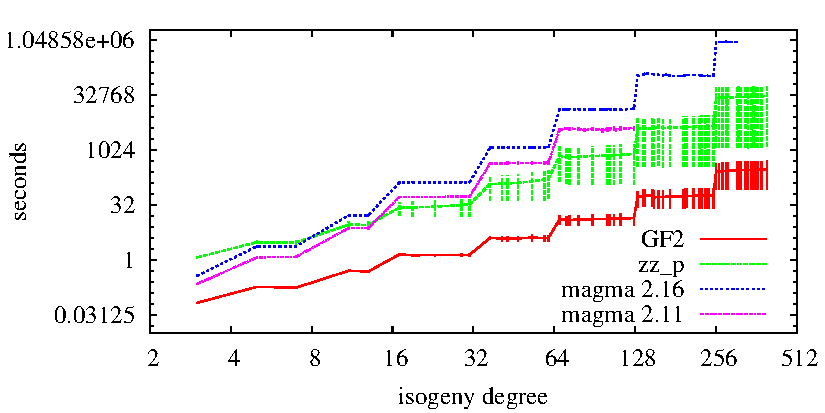
\includegraphics[width=0.9\textwidth]{isogeny/p2}
  \caption{Comparative timings for different implementations of \ctwoasfimc{} with curves defined over $\F_{2^{101}}$. Plot in logarithmic scale.}
  \label{fig:2-101}
\end{figure}

The results are in figure~\ref{fig:2-101}: we plot a line for the
average running time of the algorithm and bars around it for minimum
and maximum execution times of the final loop. Besides the dramatic
speedup obtained by using the ad-hoc type \texttt{GF2}, the
algorithmic improvements of \texttt{FAAST} over Magma are evident as
even \texttt{zz\_p} is one order of magnitude faster.

\begin{table}
  \centering
  \begin{tabular}{r r r r r r r r}
    \hline
    $\ell$ & $E[p^k]$ & $E'[p^k]$ & FI & RFR & MC & Avg tries & Avg loop time\\
    \hline
    31  &  0.3529 &  0.3529 & 0.3569 & 0.00125 & 0.00055 &  32 &   0.058\\
    61  &  0.9848 &  0.9848 & 0.8268 & 0.00343 & 0.00228 &  64 &   0.365\\
    127 &  2.6636 &  2.6626 & 1.8927 & 0.01090 & 0.00872 & 128 &   2.511\\
    251 &  6.9809 &  6.9779 & 4.2833 & 0.03092 & 0.03494 & 256 &  16.860\\
    397 & 18.1052 & 18.0952 & 9.7385 & 0.07325 & 0.14117 & 512 & 109.783\\
  \end{tabular}
  \caption{Comparative timings for the phases of \ctwoasfimc{} for curves over $\F_{2^{101}}$.}
  \label{tab:C2}
\end{table}

Table~\ref{tab:C2} shows detailed timings for each phase of
\ctwoasfimc{}. The column FI reports the time for one interpolation, the
column MC the time for one modular composition; comparing these two
columns the gain from passing from \ctwoasfi{} to \ctwoasfimc{} is
evident. Columns RFR (rational fraction reconstruction) and MC
constitute the Cauchy interpolation step that is repeated in the final
loop. The last column reports the average time spent in the loop: it
is by far the most expensive phase and this justifies the attention we
paid to FI and MC; only on some huge examples we approached the
crosspoint between these two algorithms.


\paragraph{\ctwoud{}}
\label{sec:c2-ud}
Next we ran experiments on \ctwoud{}. The first observation was that the
heuristic argument --on the probability that a degree sequence not
associated to an isogeny is not normal-- is well verified in practice:
except for a degree $2$ symmetry verified in characteristic $2$,
polynomials not associated to an isogeny very rarely gave a degree
sequence with a gap around the middle.

\pdfmcone{Added some blabla on Teske's cryptosystem.}
Looking for isogenies of unknown degree may be of some cryptographic
significance. For example, Teske's trapdoor cryptosystem selects a
binary field of composite degree ($\F_{2^{7\cdot 23}}$, in the
proposal) and chooses an elliptic curve $E$ vulnerable to the GHS
attack~\cite{gaudry+hess+smart02}. Then hides $E$ by taking a random
path of isogenies of small degrees landing on a curve $E'$ not
vulnerable to GHS, and uses $E'$ as public key. The security of the
cryptosystem comes from the assumption that it is infeasible to find a
GHS-vulnerable curve isogenous to $E'$, without the knowledge of the
isogeny path. 

The \emph{trapdoor} of the cryptosystem is the curve $E$: it is given
to a trusted authority so that --using an isogeny path from $E'$ to
$E$ and a GHS attack-- it has the power of deciphering messages at a
relatively high computational cost. This feature rests on the
assumption that it is feasible, but relatively hard, to compute any
isogeny path from $E$ to $E'$.

In this context, it may be interesting to verify that $E$ and $E'$ are
not related by an isogeny of too low degree.
From~\cite[Appendix~A]{teske06}, we took the two curves defined over
$F_{2^{161}}=\F_2[z]/(z^{161}+z^{18}+1)$ of $j$ invariants:

$1/j = z^{152} + z^{143} + z^{139} + z^{136} + z^{135} + z^{133} +
z^{130} + z^{125} + z^{124} + z^{122} + z^{120} + z^{119} + z^{118} +
z^{117} + z^{116} + z^{114} + z^{113} + z^{112} + z^{110} + z^{109} +
z^{106} + z^{105} + z^{103} + z^{102} + z^{101} + z^{99} + z^{97} +
z^{96} + z^{92} + z^{91} + z^{88} + z^{87} + z^{86} + z^{85} + z^{81}
+ z^{78} + z^{77} + z^{76} + z^{75} + z^{73} + z^{71} + z^{69} +
z^{68} + z^{67} + z^{66} + z^{63} + z^{59} + z^{58} + z^{53} + z^{51}
+ z^{50} + z^{49} + z^{48} + z^{46} + z^{45} + z^{44} + z^{42} +
z^{38} + z^{34} + z^{3} + z^{32} + z^{31} + z^{29} + z^{27} + z^{26} +
z^{24} + z^{23} + z^{22} + z^{21} + z^{20} + z^{19} + z^{18} + z^{17}
+ z^{16} + z^{15} + z^{14} + z^{13} + z^{12} + z^{10} + z^{7} + z^{6}
+ z^{4} + z^{3} + z^{2}$,

$1/j'=z^{160} + z^{156} + z^{155} + z^{153} +z^{152} +z^{151} +z^{150}
+z^{149} +z^{148} +z^{147} +z^{146} +z^{145} +z^{143} +z^{142}
+z^{141} +z^{130} +z^{129} + z^{127} + z^{126} + z^{125} + z^{124} +
z^{123} + z^{120} + z^{118} + z^{112} + z^{109} + z^{104} + z^{103} +
z^{102} + z^{101} + z^{99} + z^{98} +z^{97} +z^{96} +z^{93} +z^{92}
+z^{91} +z^{90} +z^{88} +z^{85} +z^{83} +z^{77} +z^{74} +z^{70}
+z^{68} +z^{65} +z^{64} +z^{63} + z^{62} + z^{61} + z^{60} + z^{58} +
z^{57} + z^{55} + z^{50} + z^{48} + z^{45} + z^{41} + z^{38} + z^{37}
+ z^{36} + z^{33} + z^{31} + z^{30} + z^{27} +z^{26} +z^{24} +z^{23}
+z^{22} +z^{21} +z^{20} +z^{19} +z^{17} +z^{16} +z^{14} +z^{13}
+z^{10} +z^{8} +z^{7} +z^{4} +z^{3} +z$.

We ran our two variants of \ctwoud{} on the two curves to certify the
conjectured property that no unexpected isogeny of low degree exists
between the two curves.

In 258 cpu-hours we were able to prove that no isogeny of degree
$p^c\ell$ for $\ell<2^{11}$ and $c$ arbitrary exists between the two
curves; in 694 cpu-hours we were able to prove that no isogeny of
degree less than $2^{13}$ exists either. We stress the fact that,
albeit of little interest, this computation would have been impossible
without the (surprising) discovery of \ctwoud{}.


\paragraph{Couveignes vs. Lercier-Sirvent}
Finally, we ran experiments on
\titleref{alg:le-si}. 
Table~\ref{tab:ls} shows
timings for the different phases of the algorithm for some isogeny
degrees. The first column is the time spent to find a root of
$\Modpol_\ell(X,j_E)$ in $\F_q$, the second column summarizes the time
spent to lift this root in $\Q_q$ and apply Elkies'
formulas. DiffSolve is the time spent solving the differential
equation, it is clearly the most expensive phase, although not the
most important asymptotically. RFR is the time for rational fraction
reconstruction, its rapid growth is justified by the fact that we
implemented it on top of a quadratic XGCD algorithm.

\begin{table}
  \pdfmcthree{This table has changed.}
  \centering
  \begin{tabular}{r r r r}
    \hline
    $\ell$ & Lift & DiffSolve & RFR\\
    \hline
    31  &   0.570 &   14.830 & 0.010\\
    103 &   5.160 &  274.550 & 0.250\\
    149 &  12.510 &  815.320 & 0.590\\
    239 &  21.420 & 1470.240 & 1.950\\
    331 & 113.500 & 4204.610 & 4.890\\
    389 & 147.340 & 5166.730 & 7.360\\
  \end{tabular}
  \caption{Comparative timings for the phases of \titleref{alg:le-si} 
    for curves over $\F_{3^{64}}$.}
  \label{tab:ls}
\end{table}


\begin{figure}
  \centering
  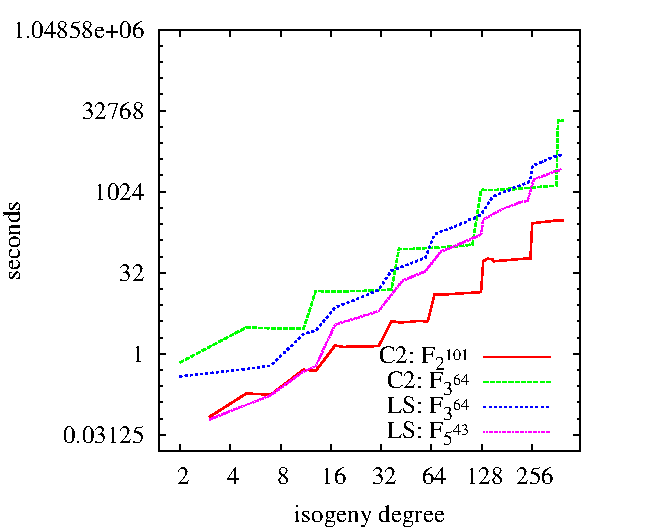
\includegraphics[height=0.45\textwidth]{isogeny/C2-LS}
  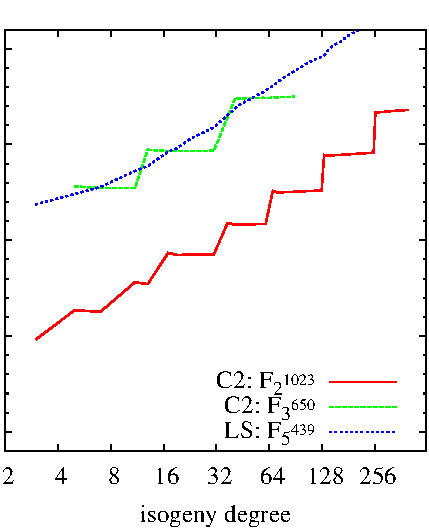
\includegraphics[height=0.45\textwidth]{isogeny/C2-LS2}
  \caption{Comparative timings for \ctwoasfimc{} (C2) and
    \titleref{alg:le-si} (LS) over different curves. Plot in
    logarithmic scale.}
  \label{fig:comp}
\end{figure}

We also compared the running times of \ctwoasfimc{} and
\titleref{alg:le-si} over curves of half the cryptographic size in
figure~\ref{fig:comp} (left) and five times the cryptographic size in
figure~\ref{fig:comp} (right). We only plot average times for \ctwo{},
in characteristic $2$ we only plot the timings for \texttt{GF2}. From
the plot it is clear that \ctwoasfimc{} only performs better than
\titleref{alg:le-si} for $p=2$, but in this case Lercier's
algorithm~\cite{lercier96} is much faster.  Contradicting theory, the
asymptotic behavior of \titleref{alg:le-si} looks worse than the one
of \ctwoasfimc{}; however comparing a Magma prototype to our highly
optimized implementation of \ctwoasfimc{} is somewhat unfair.

Furthermore, it is unlikely that \ctwoasfimc{} could be practical for
any $p>3$ because of its high dependence on $p$, while
\titleref{alg:le-si} scales pretty well with the characteristic as
shown in figure~\ref{fig:LSp}.

Considering that the asymptotic dependency of Couveignes' algorithm in
$\log q$ and in $p$ is worse than the one of \titleref{alg:le-si}
(compare Eq.~\eqref{eq:interp} to
Proposition~\ref{th:lercier-sirvent}), there are very few regions
where Couveignes' algorithm stays of practical or theoretical
interest.

\pdfmcone{People don't like pessimism.}  Ironically, the
techniques presented in this document were developed in view of an
efficient implementation of Couveignes' algorithm, but, for the
moment, their only practical application seems to be \ctwoud{}. Our hope
is that other interesting applications may be found in the future.

\begin{figure}
  \centering
  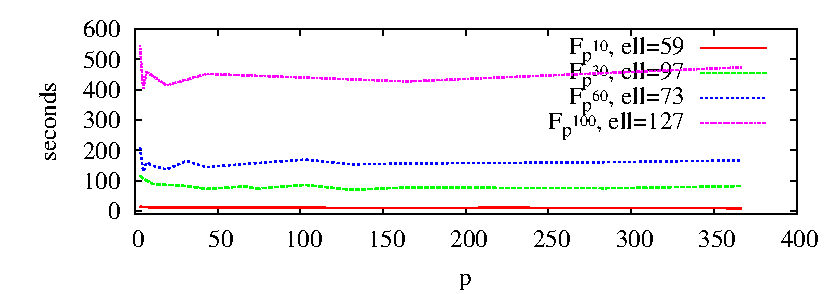
\includegraphics[width=0.9\textwidth]{isogeny/LSp}
  \caption{Timings for \titleref{alg:le-si} for different fields. We
    increase $p$ while keeping constant $d$ and the isogeny degree.}
  \label{fig:LSp}
\end{figure}


% Local Variables:
% mode:flyspell
% ispell-local-dictionary:"american"
% TeX-master: "../these"
% mode: TeX-PDF
% mode:reftex
% End:
%
% LocalWords:  Schreier Artin pseudotrace Frobenius bivariate Joux Sirvent FFT
% LocalWords:  Couveignes isogenies Schoof isogeny cryptosystems Lercier
% LocalWords:  precomputation arithmetics polylogarithmic Karatsuba precomputes
% LocalWords:  endomorphisms  isogenous



% Local Variables:
% mode:flyspell
% ispell-local-dictionary:"american"
% mode:TeX-PDF
% mode:reftex
% TeX-master: "../these"
% End:
%



\appendix
\appendixpage*
%% these.tex
%% Copyright 2010 Luca De Feo
%% All rights reserved


\chapter{Categorical considerations}
\label{cha:basic-categ-theory}

\renewcommand{\C}{\mathcal{C}}
\newcommand{\D}{\mathcal{D}}
\newcommand{\Set}{\mathbold{S\kern-0.2ex e\kern-0.2ex t}}
\newcommand{\Hask}{\mathbold{H\kern-0.2ex a\kern-0.2ex s\kern-0.2ex k}}
\newcommand{\RMod}[1]{#1\mathbold{-M\kern-0.2ex o\kern-0.2ex d}}

The aim of this chapter is to give a simpler proof of the
\hyperref[th:tellegen]{transposition theorem for arithmetic circuits}
shedding new light on it. The main idea is to bring duality back where
it belongs: category theory. This is done through the use of some
basic categorical semantics~\cite{pitts01,asperti+longo}. We also
discuss the relationship with some Haskell type classes and
perspectives for the implementation of the transposition
principle. This chapter is joint work with Boespflug.



\section{Categorical semantics of arithmetic circuits}
\label{sec:categ-semant-arithm}
\index{categorical~semantics}Categorical semantics introduce the
notion of \index{structure!valued~in~a~category}\emph{structure valued
  in a category $\C$}, which is a generalization of the concept of
\index{structure}\emph{structure} in model theory. This permits us to
reason about operations that ``preserve some algebraic structure''.
See~\cite{pitts01} for formal definitions.

Take the example of \index{arithmetic~circuit}arithmetic circuits. In
Section~\ref{sec:circuits} we defined them using left modules and
morphisms, this allowed us to state that the evaluation of a circuit
is a module morphism simply because the composition laws for
arithmetic circuits ``preserve'' the structure. Then in
Section~\ref{sec:multi} we extended the notion of circuit to embrace
circuits containing multiplication nodes; however this meant that we
had to redefine circuits from scratch, considering maps that are not
module morphisms (we did not actually write the new definition in
Section~\ref{sec:multi}, because we were lazy).

The clean way to give both definitions at once, is to consider
\index{arithmetic~circuit!valued~in~a~category}\emph{circuits valued
  in a category $\C$}.  It is soon evident that the only requirement
on the category is that it has finite products; in what follows, we
let $\C$ be a category with finite products.
  
The definition of the syntax of circuits, i.e.\ what are the nodes and
ports, how they are composed to build a circuit, etc., stay the same;
we only change the definitions of operator and of evaluation of an
arithmetic circuit.
  
\begin{definition}[Arithmetic operator, arity]
  Let $A$ be an object of $\C$.  An
  \index{arithmetic~operator}\emph{arithmetic operator} over $A$ is an
  arrow $f:\prod^iA\ra\prod^oA$ for some $i,o\in\N$. Here $i$ is
  called the \index{arity}\emph{in-arity} of $f$ or simply
  \emph{arity}, $o$ is called the \emph{out-arity} of $f$.
\end{definition}
  
\begin{definition}[Evaluation of an arithmetic circuit]
  \index{arithmetic~circuit!semantic}\index{arithmetic~circuit!evaluation}
  Let $A$ be an object of $\C$. Let $C$ be an arithmetic circuit with
  $i$ inputs and $o$ outputs, then its evaluation is an arrow
  $\eval_C:\prod^iA\ra\prod^oA$.
  
  In order to define it, we simultaneously define the evaluation
  $\eval_v$ of each $v\in V$ and the evaluation $\eval_e$ of each
  $e\in E$. We will denote by $<_v$ the orders on the input and the
  output ports of $v$.
  \begin{itemize}
  \item Let $v\in V$ have out-degree $n$, let its evaluation be
    $\eval_v:\prod^iA\ra\prod^nA$ and let $\pi_1,\ldots,\pi_n$ be the
    canonical projections from $\prod^nA$ to $A$. Let
    $o_1<_v\cdots<_vo_n$ be the output ports of $v$ and let
    $e_j=\bigl(o_j,E(o_j)\bigr)$ be the corresponding edges stemming
    from $v$, then $\eval_{e_j} = \pi_j\circ\eval_v$ for any $j$.
  \item Let $x_1<_i\cdots<_ix_i$ be the input nodes and let
    $\pi_1,\ldots,\pi_i$ be the canonical projections from $\prod^iA$
    to $A$, then $\eval_{x_j}=\pi_j$ for any $j$.
  \item For every evaluation node $v$ with in-degree $m$, let
    $i_1<_v\cdots<_vi_m$ be the input ports of $v$ and let
    $e_j=\bigl(E^{-1}(i_j),i_j\bigr)$ be the corresponding edges
    incident to $v$, then
    \begin{equation}
      \eval_v = \beta(v) \circ (\eval_{e_1}\times\cdots\times\eval_{e_m})
      \text{.}
    \end{equation}
  \item For every output node $y$, let $e\in E$ be the only edge
    incident to $y$, then $\eval_y=\eval_e$.
  \end{itemize}
    
  We can finally define $\eval_C:\prod^iA\ra\prod^oA$. Let
  $y_1<_o\cdots<_oy_o$ be the output nodes, then
  \begin{equation}
    \eval_C = \left(\eval_{y_1}\times\cdots\times\eval_{y_o}\right)
    \text{.}
  \end{equation}
  We also say that $C$ \emph{computes} $\eval_C$.
\end{definition}
  
As the reader will have noticed, we have simply taken
Definition~\ref{def:eval} and changed direct sums with categorical
products. Hence, the fact that the evaluation of a circuit in the
category of left modules is a left module morphism is now tautology;
but we can also consider circuits valued in $\Set$, then all
the theory of Section~\ref{sec:multi} can be carried out on those
circuits.
  


\section{Coevaluation}
When dealing with a construction in category theory, it is natural to
simultaneously study its dual, that is the construction obtained by
\emph{reversing all the arrows}. If in definition \ref{def:eval} we
substitute the product $\prod^nR$ by its dual $\coprod^nR$, we obtain
a new way of evaluating an arithmetic circuit that we will call
\emph{coevaluation}. In this section we let $\mathcal{D}$ be a
category with finite coproducts.

An arithmetic cobasis is just an arithmetic basis in $\D^\op$, and the
coevaluation of an arithmetic circuit is just its evaluation in
$\D^\op$. For completeness, we give the detailed definitions.

\begin{definition}[Arithmetic co-operator, arity]
  Let $A$ be an object of $\D$.  An \emph{arithmetic co-operator} over
  $A$ is an arrow $f:\coprod^iA\ra\coprod^oA$ for some $i,o\in\N$.
\end{definition}

\begin{definition}[coevaluation of an arithmetic circuit]
  \label{def:coeval}
  Let $A$ be an object of $\D$.  Let $C$ be an arithmetic circuit with
  $i$ inputs and $o$ outputs over a cobasis $\mathcal{B}$. Its
  coevaluation is an arrow $\lave_C:\coprod^iA\ra\coprod^oA$.

  We use the same notation as in the previous definition. As we did
  there, we simultaneously define $\lave_v$ for each $v\in V$ and
  $\lave_e$ for each $e\in E$.
  \begin{itemize}
  \item Let $v\in V$ have in-degree $m$, let its coevaluation be
    $\lave_v:\coprod^mA\ra\coprod^oA$ and let $\iota_1,\ldots,\iota_n$ be the
    canonical injections from $A$ to $\coprod^mA$. Let $i_1<_v\cdots<_vi_m$
    be the input ports of $v$ and let
    $e_j=\bigl(i_j,E^{-1}(i_j)\bigr)$ be the corresponding edges
    incident to $v$, then $\lave_{e_j} = \lave_v\circ\iota_j$ for any
    $j$.
  \item Let $y_1<_V\cdots<_Vy_n$ be the output nodes and let
    $\iota_1,\ldots,\iota_o$ be the canonical injections from $A$ to
    $\coprod^oA$, then $\lave_{y_j}=\iota_j$ for any $j$.
  \item For every evaluation node $v$ with out-degree $n$, let
    $o_1<_v\cdots<_vo_n$ be the output ports of $v$ and let
    $e_j=\bigl(E(o_j),o_j\bigr)$ be the corresponding edges
    stemming from $v$, then
    \begin{equation}
      \label{eq:lave_v}
      \lave_v = (\lave_{e_1}+\cdots+\lave_{e_n}) \circ \beta(v) 
      \text{.}
    \end{equation}
  \item For every input node $x$, let $e\in E$ be the only edge
    stemming from $x$, then $\lave_x=\lave_e$.
  \end{itemize}

  We can finally define $\lave_C:\coprod^iA\ra\coprod^oA$. Let
  $x_1<_V\cdots<_Vx_i$ be the input nodes, then
  \begin{equation}
    \label{eq:lave}
    \lave_C = \lave_{x_1}+\cdots+\lave_{x_i}
    \text{.}
  \end{equation}
\end{definition}

The coevaluation in general does not attach the same semantics to a
circuit as the evaluation. For example in the case of $\Set$
the coevaluation is a function from the disjoint union of $i$ copies
of $A$ to the disjoint union of $o$ copies of $A$. We can regard
circuits over cobases in $\Set$ as objects that are fed one
single element of $A$ on one out of their $n$ inputs and then take
decisions depending on which input was fed. An example is given in
figure \ref{fig:coffee}.

\begin{figure}[!ht]
  \centering
  
  \begin{tikzpicture}
    \tikzstyle{node}=[circle,thick,draw=black,minimum size=4mm]
    \tikzstyle{arg}=[rectangle,thin,draw=black,minimum size=4mm]

    \begin{scope}
      \node[arg](in){$x$};

      \node[node,below of=in](s10){$>_{10}$};

      \node[node,right of=s10,xshift=2mm](s20){$>_{20}$};
      \node[arg,below of=s10](o10){$10$c};

      \node[node,right of=s20,xshift=2mm](s50){$>_{50}$};
      \node[arg,below of=s20](o20){$20$c};

      \node[node,right of=s50,xshift=2mm](s1){$>_{100}$};
      \node[arg,below of=s50](o50){$50$c};

      \node[arg,below of=s1](o1){$1$\euro};
      \node[arg,right of=o1](o2){$2$\euro};

      \path[->]
      (in) edge (s10)
      (s10) edge (o10)
      (s10) edge (s20)
      (s20) edge (o20)
      (s20) edge (s50)
      (s50) edge (o50)
      (s50) edge (s1)
      (s1) edge (o1)
      (s1) edge (o2);
    \end{scope}
  \end{tikzpicture}  
  
  \caption{The coffee machine circuit. On input $n\in\Z$, the operator
    $>_x:\Z\ra\Z\uplus\Z$ gives $n$ on its right output if $n>x$,
    on its left output otherwise. The circuit is an euro coin
    separator.}
  \label{fig:coffee}
\end{figure}

In some cases, howevever, evaluation and coevaluation coincide. Recall
that an \emph{additive category} is a category if every hom-set is an
Abelian group, composition of morphisms is bilinear, and every finite
biproduct exists~\cite[VIII.2]{mclane}. In particular, in an additive
category finite products and coproducts are isomorphic.

\ifafourps\pagebreak[2]\fi
\begin{lemma}
  \label{th:coeval}
  Let $C$ be a circuit valued in an additive category, then
  $\eval_C\isom\lave_C$ naturally.
\end{lemma}
We just sketch the proof.
\begin{proof}
  First observe that since products and coproducts are naturally
  isomorphic, the basis of $C$ can be interpreted both as a basis and
  a cobasis. Hence both evaluation and coevaluation $C$ are
  meaningful.

  Then, we proceed by induction on the size of the circuit. First, it
  is obvious that for circuits with one unique evaluation node $v$ we
  have $\eval_C\isom\beta(v)\isom\lave_C$. Now if $C$ has $n$
  evaluation nodes, we choose any topological order on $C$ and remove
  the last evaluation node $v$ and the output nodes connected to
  it. This new circuit satisfies the lemma by induction. The claim
  follows by connecting $v$ back to the circuit.
\end{proof}


\section{The tranposition theorem}
\label{sec:tranposition-theorem}
We restate the notion of \hyperref[def:dual]{dual circuit} in our new
context. The dual circuit is obtained by reversing all the arrows, and
it is valued in the opposite category $\C^\op$. Although we use the
same notation, the reader shall not confuse this definition of the
dual circuit $C^\op$ with the definition of the \emph{opposite
  circuit} we gave in Section~\ref{sec:bilinear-chains}.

\begin{definition}[Dual basis]
  Let $A$ be an object of $\C$ and let $\mathcal{B}$ be an arithmetic
  basis over $A$. We define the dual basis $\mathcal{B}^\op$ as
  \begin{equation}
    \mathcal{B}^\op= \{f^\op \,|\, f\in\mathcal{B}\}
    \text{.}
  \end{equation}
\end{definition}

\begin{definition}[Dual circuit]
  \index{arithmetic~circuit!dual} Let $A$ be an object of $\C$. Let
  ${C=(V,E,\le,\le_i,\le_o)}$ be a circuit over $(A,\mathcal{B})$. For
  any $v\in V$ define
  \begin{equation}
    v^\op =
    \begin{cases}
    (O,I,f^\op)              &\text{if $v=(I,O,f)$ with $f\ne\emptyset$,}\\
    (O,\emptyset,\emptyset) &\text{if $v=(\emptyset,O,\emptyset)$,}\\
    (\emptyset,I,\emptyset) &\text{if $v=(I,\emptyset,\emptyset)$.}
    \end{cases}
  \end{equation}

  The \emph{dual circuit} of $C$, denoted by $C^\op$, is the circuit
  over $(A,\mathcal{B}^\op)$ defined as
  \[C^\op = (V^\op, E^{-1},\le^\op,\le_i',\le_o')\text{,}\]
  where $V^\op=\{v^\op|v\in V\}$ and the orderings are defined
  as follows:
  \begin{align}
    v \le v' \;&\Leftrightarrow\; {v'}^\op \le^\op {v}^\op\text{,}\\
    v \le_o v' \;&\Leftrightarrow\; {v}^\op \le_o' {v'}^\op\text{,}\\
    v \le_i v' \;&\Leftrightarrow\; {v}^\op \le_i' {v'}^\op\text{.}
  \end{align}
\end{definition}


We now have all the elements to prove the transposition theorem. We
let $\C$ and $\C'$ be categories with finite products.  The first,
trivial, observation is that certain functors ``preserve'' the
semantic of a circuit. If $F:\C\ra\C'$ is a functor, we define by
$F(\mathcal{B})$ the basis obtained by substituting any arrow $f$ with
$F(f)$, and by $F(C)$ the circuit obtained by substituting any node
with the corresponding node in $F(\mathcal{B})$.

\begin{proposition}
  Let $F:\C\ra\C'$ be a continuous functor (i.e.\ a functor that
  preserves small limits; we actually only need it to preserve
  products). Let $C$ be a circuit valued in $\C$. Then $F(C)$ is
  valued in $\C'$ and $F(\eval_C)=\eval_{F(C)}$.
\end{proposition}

\begin{corollary}
  Let $\C$ be a category with finite products, $\D$ a category with
  finite coproducts and $F:\C\ra\D^\op$ a continuous functor. Then
  $F(C)^\op$ is valued in $\D$ and $F(\eval_C)^\op=\lave_{F(C)^{\op}}$.
\end{corollary}

\begin{corollary}[Transposition theorem]
  Let $\C$ be an additive category and let $F:\C\ra\C^\op$ be a
  continuous functor. Then $F(\eval_{C})^\op\isom\eval_{F(C)^\op}$.
\end{corollary}

The transposition theorem of Section~\ref{sec:tellegen}, then follows
by considering the transposition functor
$\dual{()}:\RMod{R}\ra\RMod{R}$ (note that the transposition
functor is traditionally written in a contravariant fashion).


\section{From circuits to function-level programming}
\label{sec:fp}
\index{arrow}
\lstset{language=haskell} People who think that categories are just
abstract nonsense, may be surprised discovering that arithmetic
circuits valued in $\Hask$ (the category of Haskell types) are
already implemented in Haskell. Alternatively, they might think that
Haskell is concrete nonsense.

The package \lstinline+Control.Arrow+ implements what are commonly
called \emph{arrows} in Haskell jargon. Arrows were introduced
in~\cite{hughes98} as a generalization of \emph{monads}, they have
been successfully applied to many different settings such as, for
example, solving ordinary differential
equations~\cite{liu+hudak10}. Paterson~\cite{paterson01} was the first
to realize the relationship between circuits and arrows, and to
propose a DSL for arrows that is amazingly similar to straight line
programs.

The standard library class \lstinline+Arrow+ is roughly equivalent to
arithmetic circuits valued in $\Hask$ (or $\Set$),
while \lstinline+ArrowChoice+ is roughly equivalent to arithmetic
circuits valued in $\Hask^\op$. So we asked ourselves the
question of whether it is possible to write a type class
\lstinline+AdditiveArrow+ that has the same properties of circuits
valued in additive categories. A desirable feature of \emph{additive
  arrows} is that they could be evaluated both in $\C$ and $\C^\op$,
thus they share some similarities with \emph{invertible
  arrows}~\cite{alimarine+al:invertible-arrows}.

We sketch what an additive arrow should look like, by giving an
hypothetical list of type classes;
following~\cite{yorgey:typeclassopedia}, we use infix operators
\lstinline+(~>)+ instead of prefix ones as in the standard Haskell
library.  As for arrows, we start from the class \lstinline+Category+.

\begin{lstlisting}
  class Category (~>) => where
    id :: (a ~> a)
    (.) :: (b ~> c) -> (a ~> b) -> (a ~> c)
\end{lstlisting}

In order to behave as a category, an instance of this class shall form
a monoid for the operation \lstinline+(.)+, with \lstinline+id+ being
the identity element. Now this class can be extended to model additive
categories: we first define a class that mimics \emph{Ab-categories},
or \emph{preadditive} categories, that is categories whose hom-sets
are Abelian groups, then we define additive categories.

\begin{lstlisting}
  class Category (~>) => AbCategory (~>) where
    zeroArrow :: (a ~> b)
    (<+>) :: (a ~> b) -> (a ~> b) -> (a ~> b)
\end{lstlisting}

\begin{lstlisting}
  class AbCategory (~>) => AdditiveCategory (~>) where
    (&&&) :: (a ~> b) -> (a ~> c) -> (a ~> (b, c))
    (|||) :: (a ~> c) -> (b ~> c) -> ((a, b) ~> c)
    (***) :: (a ~> b) -> (c ~> d) -> ((a, c) ~> (b, d))
\end{lstlisting}

Where \lstinline+&&&+ roughly corresponds to the operator $\hub$ of
arithmetic circuits, \lstinline+|||+ corresponds to $+$, and
\lstinline+***+ corresponds to forming a new circuit by putting two
circuits side by side.

However, these type classes cannot be implemented as expected because
Haskell tuples do not behave like $R^n$: in particular, it is
impossible to properly implement the operators \lstinline+|||+ and
\lstinline+***+ on tuples. To circumvent this, we have to use some
form of dependent types~\cite{kiselyov+lammel+schupke04,mcbride01} to
encode the free module $R^{n+m}$ and its projections over $R^n$ and
$R^m$.

After some unsuccessful experiments with GADT's, we succeeded in
implementing additive circuits in the category of $\Z$-modules and
transposable multiplication in $\Z[X]$ using type level arithmetic
from the package \lstinline+Data.TypeLevel+. We thank Jacques Carette
for having suggested this solution to us.

The source code is presented in the next section. Notice, however that
our implementation needs to suggest some trivialities to the type
checker (for example, $a\le a+b$ for any $b\in\N$) in order for the
compilation to succeed. 

Another problem is that the implementation of polynomial
multiplication is far from being self-evident. In fact, we had to
follow Kiselyov and
Peyton-Jones~\cite{jones+kiselyov:advanced+overlap08} to implement
\emph{advanced overlapping instances}.

Future research directions include:
\begin{itemize}
\item use a language natively implementing dependent data types to
  avoid hacks;
\item implement a DSL similar to Paterson's do-notation for
  arrows~\cite{paterson01}.
\end{itemize}
Our hope is that these techniques could provide an efficient and easy
to use library for automated theorem provers, to prove the correctness
of programs based on the transposition principle.


\section[\emph{Self-transposing} polynomial
multiplication]{Implementation of \emph{self-transposing} polynomial
  multiplication in Haskell}
\label{sec:impl-emphs-transp}
\pdfmcthree{What a gaffe! This code implements naive multiplication, not Karatsuba's.}

\begin{xcomment}{lstlisting}
\input{trans/transkara.hs}
\end{xcomment}



\renewcommand{\C}{\mathbb{C}}



% Local Variables:
% mode:flyspell
% ispell-local-dictionary:"american"
% mode:TeX-PDF
% mode:reftex
% TeX-master: "../these"
% End:
%

\chapter{Linearity inference of karatsuba multiplication}
\label{cha:line-infer-karats}

\lstset{language=haskell}

We show here an example of inference of linearity in Haskell, using
the technique described in Section~\ref{sec:inference}. We define type
classes \lstinline{Ring} and \lstinline{Module} to represent
left-linear operations on rings and free modules. We instantiate them
with integers as base ring, and lists of integers as free module
(representing polynomials over $\Z[X]$).

We implement Karatsuba multiplication over $\Z[X]$, using only the
methods defined in \lstinline{Ring} and \lstinline{Module}. This
allows the type checker to deduce that Karatsuba multiplication is
linear in its first argument, once the second argument and the degree
of the polynomials are fixed. The code makes use of functional
dependencies, it must be run with the switch \verb|-fglasgow-exts| on.

\begin{xcomment}{lstlisting}
\chapter{Linearity inference of karatsuba multiplication}
\label{cha:line-infer-karats}

\lstset{language=haskell}

We show here an example of inference of linearity in Haskell, using
the technique described in Section~\ref{sec:inference}. We define type
classes \lstinline{Ring} and \lstinline{Module} to represent
left-linear operations on rings and free modules. We instantiate them
with integers as base ring, and lists of integers as free module
(representing polynomials over $\Z[X]$).

We implement Karatsuba multiplication over $\Z[X]$, using only the
methods defined in \lstinline{Ring} and \lstinline{Module}. This
allows the type checker to deduce that Karatsuba multiplication is
linear in its first argument, once the second argument and the degree
of the polynomials are fixed. The code makes use of functional
dependencies, it must be run with the switch \verb|-fglasgow-exts| on.

\begin{xcomment}{lstlisting}
\chapter{Linearity inference of karatsuba multiplication}
\label{cha:line-infer-karats}

\lstset{language=haskell}

We show here an example of inference of linearity in Haskell, using
the technique described in Section~\ref{sec:inference}. We define type
classes \lstinline{Ring} and \lstinline{Module} to represent
left-linear operations on rings and free modules. We instantiate them
with integers as base ring, and lists of integers as free module
(representing polynomials over $\Z[X]$).

We implement Karatsuba multiplication over $\Z[X]$, using only the
methods defined in \lstinline{Ring} and \lstinline{Module}. This
allows the type checker to deduce that Karatsuba multiplication is
linear in its first argument, once the second argument and the degree
of the polynomials are fixed. The code makes use of functional
dependencies, it must be run with the switch \verb|-fglasgow-exts| on.

\begin{xcomment}{lstlisting}
\input{trans/haskatsuba.hs}
\end{xcomment}


                  

% Local Variables:
% mode:flyspell
% ispell-local-dictionary:"american"
% mode:TeX-PDF
% mode:reftex
% TeX-master: "../these"
% End:
%

\end{xcomment}


                  

% Local Variables:
% mode:flyspell
% ispell-local-dictionary:"american"
% mode:TeX-PDF
% mode:reftex
% TeX-master: "../these"
% End:
%

\end{xcomment}


                  

% Local Variables:
% mode:flyspell
% ispell-local-dictionary:"american"
% mode:TeX-PDF
% mode:reftex
% TeX-master: "../these"
% End:
%

\chapter{Proof of Vélu's formulas}
\label{cha:proof-velus-formulas}

I always had admiration for my colleagues who can develop by hand two
pages full of computations without making mistakes. Concerning me, I
usually make a sign mistake at the third term. Tired of having to
check for sign errors in other people's papers any time I had to use
Vélu formulas, I decided to make an automatic proof of it.

The following Magma code proves the passage from Eq.~\eqref{eq:155} to
Eq.~\eqref{eq:161} and from there to~\eqref{eq:157}.

\begin{xcomment}{lstlisting}
\chapter{Proof of Vélu's formulas}
\label{cha:proof-velus-formulas}

I always had admiration for my colleagues who can develop by hand two
pages full of computations without making mistakes. Concerning me, I
usually make a sign mistake at the third term. Tired of having to
check for sign errors in other people's papers any time I had to use
Vélu formulas, I decided to make an automatic proof of it.

The following Magma code proves the passage from Eq.~\eqref{eq:155} to
Eq.~\eqref{eq:161} and from there to~\eqref{eq:157}.

\begin{xcomment}{lstlisting}
\chapter{Proof of Vélu's formulas}
\label{cha:proof-velus-formulas}

I always had admiration for my colleagues who can develop by hand two
pages full of computations without making mistakes. Concerning me, I
usually make a sign mistake at the third term. Tired of having to
check for sign errors in other people's papers any time I had to use
Vélu formulas, I decided to make an automatic proof of it.

The following Magma code proves the passage from Eq.~\eqref{eq:155} to
Eq.~\eqref{eq:161} and from there to~\eqref{eq:157}.

\begin{xcomment}{lstlisting}
\input{isogeny/veluproof.mgm}
\end{xcomment}

The first and second line of output are the differences between each
term of the sums in Eqs.~\eqref{eq:155} and~\eqref{eq:161}. In both
lines, to conclude one must observe that all the terms in the
difference contain an odd power of $y(Q)$, thus they sum up to $0$
over $G^\ast$.

The third line is the difference between each term of the sums in
Eqs.~\eqref{eq:161} and~\eqref{eq:157}. The result is
self-explanatory.


% Local Variables:
% mode:flyspell
% ispell-local-dictionary:"american"
% mode:TeX-PDF
% mode:reftex
% TeX-master: "../these"
% End:

\end{xcomment}

The first and second line of output are the differences between each
term of the sums in Eqs.~\eqref{eq:155} and~\eqref{eq:161}. In both
lines, to conclude one must observe that all the terms in the
difference contain an odd power of $y(Q)$, thus they sum up to $0$
over $G^\ast$.

The third line is the difference between each term of the sums in
Eqs.~\eqref{eq:161} and~\eqref{eq:157}. The result is
self-explanatory.


% Local Variables:
% mode:flyspell
% ispell-local-dictionary:"american"
% mode:TeX-PDF
% mode:reftex
% TeX-master: "../these"
% End:

\end{xcomment}

The first and second line of output are the differences between each
term of the sums in Eqs.~\eqref{eq:155} and~\eqref{eq:161}. In both
lines, to conclude one must observe that all the terms in the
difference contain an odd power of $y(Q)$, thus they sum up to $0$
over $G^\ast$.

The third line is the difference between each term of the sums in
Eqs.~\eqref{eq:161} and~\eqref{eq:157}. The result is
self-explanatory.


% Local Variables:
% mode:flyspell
% ispell-local-dictionary:"american"
% mode:TeX-PDF
% mode:reftex
% TeX-master: "../these"
% End:


\backmatter
\ifafour \addtocontents{toc}{\clearpage} \fi  % Fix this horrible table
\chapter{Conclusion}

\pdfmctwo{Conclusion.}
We have presented our contributions to the study of efficient
algorithms for towers of finite fields and isogenies between elliptic
curves. In view of these applications, we have employed advanced
algebraic and algorithmic techniques, and developed new tools that
have an interest of their own. Our contributions span three directions.

\paragraph{Transposition principle}
Before this work, the transposition principle used to be regarded
merely as an existential result about algebraic algorithms.
Following~\cite{bostan+lecerf+schost:tellegen}, it could be applied in
an automatic fashion to a very special class of algebraic algorithms,
that we call \emph{algebraic transforms} in
Section~\ref{sec:stra-line-progr}. More general algebraic algorithms,
such as polynomial multiplication or Euclidean division, were
previously treated case-by-case.

In this document we have shown that typed functional languages allow
to automatically infer the linear algebraic structure of any algebraic
algorithm. Once this structure is known, the transposition of the
algebraic algorithm is automatically produced by partial evaluation.
It would be interesting to explore new ways of implementing the
transposition principle in higher order languages such as Haskell or
Coq, as this could have applications to the formal verification of
computer algebra systems by automated theorem provers.  We have
sketched some relevant ideas in Appendix~\ref{cha:basic-categ-theory}.

\paragraph{Towers of finite fields}
With the help of transposed algorithms, we have constructed a family
of Artin-Schreier towers of finite fields with quasi-optimal
arithmetic operations. Thanks to Couveignes'
algorithm~\cite{couveignes00}, such fast arithmetics generalize to any
Artin-Schreier tower.

Since any separable extension of degree equal to the characteristic is
Artin-Schreier, our construction provides --at least in theory-- fast
arithmetics for any such tower of extensions.  This can be applied,
for example, to the computation of torsion points of Abelian
varieties, as we did in this document. It would be interesting to
generalize this construction to the case of function fields, as this
could have applications to coding
theory~\cite{garcia+stichtenoth96,shum-et-al01}.

\paragraph{Elliptic curves}
Using our construction for Artin-Schreier towers, we were able to give
the first complete implementation of Couveignes' second algorithm for
isogeny computation~\cite{couveignes96}. This, together with a further
improvement we have presented in Section~\ref{sec:C2-AS-FI}, yields an
algorithm whose complexity is quadratic in the degree of the isogeny.

The comparison of our implementation with Lercier and Sirvent's
algorithm~\cite{lercier+sirvent08} concludes in favor of the latter,
however our improvements to Couveignes' algorithm stay of theoretical
interest for several reasons. First, Couveignes' algorithm can be
easily generalized to Jacobians of hyperelliptic curves, although with
a much worse complexity. Improving such generalization, at least for
the case of genus $2$ hyperelliptic curves, would be of some relevance
for point counting~\cite{schoof95,pila90,gaudry+schost04}; although
$p$-adic methods are likely to remain the best algorithms for the
small characteristic
case~\cite{kedlaya01,denef+vercauteren06}. 

Second, our generalization of Couveignes' algorithm to compute
isogenies of unknown degree sheds new light on Couveignes' algorithm
and on the complexity of the isogeny computation problem; and could
have applications in
cryptography~\cite{teske06,rostovtsev+stolbunov06}.  Looking for
similar generalizations of other algorithms, such as Couveignes' first
algorithm~\cite{couveignes94}, is a first step towards a better
understanding of the problem, and could ultimately lead to an optimal
algorithm to compute isogenies of given degree between elliptic
curves: a result that is still out of reach today.


%%% Local Variables: 
%%% mode:flyspell
%%% ispell-local-dictionary:"american"
%%% mode:reftex
%%% TeX-master: "../these"
%%% mode: PDFLaTex
%%% End: 

\listofsymbols[5em]
\printindex
\bibliographystyle{amsalpha}
\bibliography{defeo}

\thirdcover
\fourthcover
\subsection*{Abstract}
In this thesis we apply techniques from computer algebra and language
theory to speed up the elementary operations in some specific towers
of finite fields. We apply our construction to the problem of
computing isogenies between elliptic curves and obtain faster (both
asymptotically and in practice) variants of Couveignes' algorithm.

After some preliminaries, we introduce in Part II one of our main
tools: transposition of linear programs. Previously, Bostan, Schost
and Lecerf had shown that transposition of programs is possible,
without losses in time and space complexity, in a slightly generalized
straight-line-program model. We generalize their construction and
devise a fully featured functional language together with an algorithm
to transpose programs written in it. Our new transposition is as
efficient as theirs on programs that fit into their model, but it also
permits to treat more generic programs with a minor loss in space
complexity. We also describe the implementation of a compiler
materializing our ideas.

In Part III, we combine our transposition method with well known
techniques coming from computer algebra and elimination theory, then
we show some new results on towers of Artin-Schreier extensions over
finite fields. This allows us to design a complete set of algorithms
to perform the most common arithmetic operations on Artin-Schreier
towers in quasi-optimal time. We implemented all our algorithms in a
software package that we describe at the end of this part.

Finally, Part IV discusses the problem of isogeny computation. We
apply our techniques to a fast variant of Couveignes' algorithm that
we had obtained in our Masters thesis, and make comparisons to other
algorithms to compute isogenies.



\selectlanguage{french}
\subsection*{Résumé}

Dans cette thèse nous appliquons des techniques provenant du calcul
formel et de la théorie des langages afin d'améliorer les operations
élémentaires dans certaines tours de corps finis. Nous appliquons
notre constructions au problème du calcul d'isogénies entre courbes
elliptiques et obtenons une variante plus rapide (à la fois en théorie
et en pratique) de l'algorithme de Couveignes.

Après avoir introduit les notions de base, nous présentons dans la
Partie II un de nos outils principaux: la transposition de programmes
linéaires. Précédemment, Bostan, Schost et Lecerf avaient prouvé qu'il
est possible transposer des programmes, sans pertes en complexité
temps ou espace, dans un modèle qui est une modeste généralisation des
programmes sans branchements. Nous généralisons leur construction en
concevant un langage fonctionnel standard pour lequel nous donnons un
algorithme de transposition. Notre nouvelle transposition est aussi
efficace que la leur sur des programmes qui font partie de leur
modèle, mais elle permet aussi de traiter des programmes plus généraux
avec des pertes mineures en complexité espace. Nous décrivons
l'implantation d'un compilateur réalisant nos idées.

Dans la Partie III, nous combinons notre transposition avec des
techniques classiques de calcul formel et théorie de l'élimination,
puis nous montrons des nouveaux résultats sur les tours
d'Artin-Schreier sur des corps finis. Ceci nous permet de concevoir
une gamme d'algorithmes qui calculent en temps quasi-optimal les
opérations arithmetiques les plus communes sur les tours
d'Artin-Schreier. Nous avons implanté ces algorithmes dans une
bibliothèque logicielle que nous décrivons à la fin de cette partie.

Enfin, la Partie IV traite le problème du calcul d'isogénies. Nous
appliques nos techniques à une variante rapide de l'algorithme de
Couveignes que nous avions proposée dans notre mémoire de Master, puis
nous comparons les résultats avec d'autres algorithmes pour le calcul
d'isogénies.

\selectlanguage{american}

% Local Variables:
% mode:flyspell
% ispell-local-dictionary:"american"
% mode:TeX-PDF
% mode:reftex
% TeX-master: "../these"
% End:
%
% LocalWords:  Schreier Artin pseudotrace frobenius bivariate Joux Sirvent FFT
% LocalWords:  Couveignes isogenies Schoof isogeny cryptosystems Lercier
% LocalWords:  precomputation arithmetics polylogarithmic Karatsuba


\end{document}


% Local Variables:
% mode:TeX-PDF
% mode:reftex
% End:
%
